% Detect and warn about obsolete latex commands.
% NAG will check for many common mistakes, and give some hints on
% what to use instead. However, you should always refer to l2tabu for a
% more detailed explanation of the whats and whys: it gives more
% information than can be possibly pressed into two lines of error
% message. Orthodox checks for pitfalls that are not technically
% incorrect. If you know what you’re doing, omit orthodox.
\RequirePackage[l2tabu, orthodox]{nag} 

% submission instructions: https://www.kcl.ac.uk/campuslife/acservices/researchdegrees/students/index

\documentclass[british,a4paper,11pt,twoside]{StyleThese}

\makeatletter
\title{Data Driven Endoscopic Camera Motion Automation}\let\thetitle\@title
\author{Martin Huber}\let\theauthor\@author
\makeatother

%%%%%%%%%%%%%%%%%%%%%%%%%%%%%%%%%%%%%%%%%%%%%%%%%
% Common tools
%%%%%%%%%%%%%%%%%%%%%%%%%%%%%%%%%%%%%%%%%%%%%%%%%
\usepackage{ifpdf}


%%%%%%%%%%%%%%%%%%%%%%%%%%%%%%%%%%%%%%%%%%%%%%%%%
% Math
%%%%%%%%%%%%%%%%%%%%%%%%%%%%%%%%%%%%%%%%%%%%%%%%%
\usepackage{amsmath} % load before txfonts
\usepackage{amssymb}


%%%%%%%%%%%%%%%%%%%%%%%%%%%%%%%%%%%%%%%%%%%%%%%%%
% Algorithms and theorems
%%%%%%%%%%%%%%%%%%%%%%%%%%%%%%%%%%%%%%%%%%%%%%%%%
%\usepackage[amsmath,thmmarks,hyperref]{ntheorem}

%\setlength{\theorempostskipamount}{15pt}

%\theoremstyle{break}
%\theoremheaderfont{\normalfont\bfseries}
%\theoremseparator{}
%\theorembodyfont{\normalfont}
%\theoremsymbol{\rule{1ex}{1ex}}
%\newtheorem{algorithm}{Algorithm}


%%%%%%%%%%%%%%%%%%%%%%%%%%%%%%%%%%%%%%%%%%%%%%%%%
% Fonts and Encoding
%%%%%%%%%%%%%%%%%%%%%%%%%%%%%%%%%%%%%%%%%%%%%%%%%
\usepackage[utf8]{inputenc}

% Use T1 font encoding
\usepackage[T1]{fontenc}

% Add a few more symbols: mu, bullet points, etc.
\usepackage{textcomp}


%%%%%%%%%%%%%%%%%%%%%%%%%%%%%%%%%%%%%%%%%%%%%%%%%
% Figures
%%%%%%%%%%%%%%%%%%%%%%%%%%%%%%%%%%%%%%%%%%%%%%%%%
%\usepackage{placeins} % for \FloatBarrier
%\usepackage[margin=10pt,font=small,labelfont=bf,tableposition=top]{caption}
%\usepackage[font=footnotesize]{subfig}
\usepackage{graphicx}


%%%%%%%%%%%%%%%%%%%%%%%%%%%%%%%%%%%%%%%%%%%%%%%%%
% Tables
%%%%%%%%%%%%%%%%%%%%%%%%%%%%%%%%%%%%%%%%%%%%%%%%%
% Correct spacing for top captions
%\usepackage{topcapt}
%\newcommand{\topcaption}{\caption}

% Tool to merge several rows
\usepackage{multirow}

% Tool to split a cell (upper left) with a diagonal line (slash)
%\usepackage{slashbox}
\usepackage{diagbox}

% Choose a smaller column separation
\setlength{\tabcolsep}{3pt}


%%%%%%%%%%%%%%%%%%%%%%%%%%%%%%%%%%%%%%%%%%%%%%%%%
% Definitions
%%%%%%%%%%%%%%%%%%%%%%%%%%%%%%%%%%%%%%%%%%%%%%%%%
\DeclareMathOperator{\Id}{Id}
\DeclareMathOperator{\Expec}{\mathbb{E}}
\DeclareMathOperator{\grad}{grad}

\newcommand{\argmax}{\operatornamewithlimits{arg\,max}}
\newcommand{\argmin}{\operatornamewithlimits{arg\,min}}
\DeclareMathOperator{\median}{median}

\DeclareMathOperator{\trace}{trace}
\DeclareMathOperator{\vect}{Vect}

\providecommand{\abs}[1]{\left\lvert#1\right\rvert}
\providecommand{\norm}[1]{\left\lVert#1\right\rVert}
\providecommand{\dotprod}[2]{\langle #1\,\vert\, #2 \rangle}
\providecommand{\dist}[2]{\operatorname{dist}\left( #1 , #2 \right)}

\providecommand{\liebracket}[2]{\left[ #1\,,\, #2 \right]}
\DeclareMathOperator{\ad}{ad}
\DeclareMathOperator{\Ad}{Ad}

\providecommand{\simil}[2]{\operatorname{Sim}\left(#1,#2\right)}
\providecommand{\similb}[3]{\operatorname{Sim}\left(#1,#2,#3\right)}
\providecommand{\reg}[1]{\operatorname{Reg}\left(#1\right)}
\providecommand{\jac}[1]{J_{\mathrm{#1}}}

\providecommand{\ud}{\mathrm{d}}

\newcommand{\ba}{\boldsymbol{a}}
\newcommand{\bA}{\boldsymbol{A}}
\newcommand{\bc}{\boldsymbol{c}}
\newcommand{\be}{\boldsymbol{e}}
\newcommand{\bff}{\boldsymbol{f}}
\newcommand{\bM}{\boldsymbol{M}}
\newcommand{\bp}{\boldsymbol{p}}
\newcommand{\br}{\boldsymbol{r}}
\newcommand{\bs}{\boldsymbol{s}}
\newcommand{\bx}{\boldsymbol{x}}
\newcommand{\by}{\boldsymbol{y}}
\newcommand{\bu}{\boldsymbol{u}}
\newcommand{\bv}{\boldsymbol{v}}
\newcommand{\bw}{\boldsymbol{w}}
\newcommand{\bW}{\boldsymbol{W}}
\newcommand{\balpha}{\boldsymbol{\alpha}}
\newcommand{\bbeta}{\boldsymbol{\beta}}
\newcommand{\bpi}{\boldsymbol{\pi}}
\newcommand{\btheta}{\boldsymbol{\theta}}
\newcommand{\bgamma}{\boldsymbol{\gamma}}
\newcommand{\bnu}{\boldsymbol{\nu}}
\newcommand{\bphi}{\boldsymbol{\phi}}
\newcommand{\bPhi}{\boldsymbol{\Phi}}
\newcommand{\bpsi}{\boldsymbol{\psi}}
\newcommand{\bPsi}{\boldsymbol{\Psi}}
\newcommand{\brho}{\boldsymbol{\rho}}
\newcommand{\bvarphi}{\boldsymbol{\varphi}}
\newcommand{\bvarsigma}{\boldsymbol{\varsigma}}
\newcommand{\btau}{\boldsymbol{\tau}}

\newcommand{\IR}{\mathbb{R}}

% Text commands
\usepackage{xspace}
% \xspace adds space at the end of a macro designed
% for use in text, unless the macro is followed by
% certain punctuation characters

\newcommand{\microns}{\textmu m\xspace}

\newcommand{\cvzr}{Cellvizio\textregistered\xspace}
\newcommand{\cvz}{Cellvizio\xspace}
\newcommand{\FCMLeica}{Leica FCM1000 microscope\xspace}

% Add a period to the end of an abbreviation unless there's one
% already, then \xspace.
\makeatletter
\DeclareRobustCommand\onedot{\futurelet\@let@token\@onedot}
\def\@onedot{\ifx\@let@token.\else.\null\fi\xspace}

\providecommand{\eg}{e.g\onedot}
\providecommand{\ie}{i.e\onedot}
\providecommand{\cf}{cf\onedot}
\providecommand{\etc}{etc\onedot}
\providecommand{\etal}{\emph{et~al}\onedot}

\makeatother


% define custom figref and secref based on eqref
\providecommand{\figref}[1]{Fig.~\ref{#1}}
\providecommand{\Figref}[1]{Figure~\ref{#1}}
\providecommand{\secref}[1]{Section~\ref{#1}}
\providecommand{\Secref}[1]{Section~\ref{#1}}
\providecommand{\chapref}[1]{Chapter~\ref{#1}}
\providecommand{\Chapref}[1]{Chapter~\ref{#1}}
\providecommand{\appref}[1]{Appendix~\ref{#1}}
\providecommand{\Appref}[1]{Appendix~\ref{#1}}

\providecommand{\algref}[1]{Algorithm~\ref{#1}}
\providecommand{\Algref}[1]{Algorithm~\ref{#1}}
\providecommand{\tabref}[1]{Table~\ref{#1}}
\providecommand{\Tabref}[1]{Table~\ref{#1}} 


% Do we want a draft note? Uncomment if not
\newcommand{\draftnote}{\textcolor[gray]{0.5}{\textbf{DRAFT -- \today}}}
%%%%%%%%%%%%%%%%%%%%%%%%%%%%%%%%%%%%%%%%%%%%%%%%%
% Custom commands
%%%%%%%%%%%%%%%%%%%%%%%%%%%%%%%%%%%%%%%%%%%%%%%%%
\DeclareMathOperator{\IM}{\mathbf{DE9IM}}
\DeclareMathOperator{\Crop}{Crop}
\DeclareMathOperator{\Warp}{Warp}
\DeclareMathOperator{\diag}{diag}
\DeclareMathOperator{\expl}{exp_{Lie}}
\DeclareMathOperator{\id}{Id}
\DeclareMathOperator{\MAD}{MAD}

\newcommand{\homogeneous}[2]{{}^{^#1}\Theta_{_#2}}
\newcommand\algoref{Algorithm~\ref}

%%%%%%%%%%%%%%%%%%%%%%%%%%%%%%%%%%%%%%%%%%%%%%%%%
% Custom settings
%%%%%%%%%%%%%%%%%%%%%%%%%%%%%%%%%%%%%%%%%%%%%%%%%
\setcounter{secnumdepth}{3}

%%%%%%%%%%%%%%%%%%%%%%%%%%%%%%%%%%%%%%%%%%%%%%%%%
% Extra packages
%%%%%%%%%%%%%%%%%%%%%%%%%%%%%%%%%%%%%%%%%%%%%%%%%
\usepackage{caption}
\usepackage{subcaption}
\usepackage{booktabs}
\usepackage{lscape}
\usepackage{natbib}
\usepackage{adjustbox}
\usepackage[ruled,vlined]{algorithm2e}
\usepackage{algpseudocode}
\usepackage{siunitx}
% \usepackage{hyperref}

%%%%%%%%%%%%%%%%%%%%%%%%%%%%%%%%%%%%%%%%%%%%%%%%%
% Layout
%%%%%%%%%%%%%%%%%%%%%%%%%%%%%%%%%%%%%%%%%%%%%%%%%
\usepackage[left=1.5in,right=1.3in,top=1.1in,bottom=1.1in,includefoot,includehead,headheight=13.6pt]{geometry}
% Use 1.5 line spacing. UCL says
% "Double or one-and-a-half spacing should be used in typescripts,
% except for indented quotations or footnotes where single spacing may
% be used."
\usepackage{setspace}
\onehalfspace

% Draft note
% No draft note (empty one) by default
\providecommand{\draftnote}{}

% Fancy Header and Footer
\usepackage{fancyhdr}
\pagestyle{fancy} % Sets fancy header and footer

\fancyhf{} % clear all header and footer fields

% line width used to draw the header line
\renewcommand{\headrulewidth}{1.0pt}

\makeatletter

% redefines chapter marks to use
% the chapter number only in mainmatter
\def\chaptermark#1{%
 \markboth {\MakeUppercase{%
 \ifnum \c@secnumdepth >\m@ne
  \if@mainmatter
   \@chapapp\ \thechapter. \ %
  \fi
 \fi
#1}}
{\ifnum \c@secnumdepth >\m@ne
  \if@mainmatter
   \@chapapp\ \thechapter. \ %
  \fi
 \fi
#1}}%

\if@twoside
 % Page number (boldface) in left on even
 % pages and right on odd pages
 \fancyhead[LE,RO]{\bfseries\thepage}
 % Chapter in the right on even pages
 \fancyhead[RE]{\bfseries\nouppercase{\leftmark}}
 % Section in the left on odd pages
 \fancyhead[LO]{\bfseries\nouppercase{\rightmark}}

 % Draft mark
 \fancyfoot[LE,RO]{\draftnote}

 % Page number and draft mark on plain pages
 \fancypagestyle{plain}{
   \fancyhf{} % clear all header and footer fields
   \fancyfoot[C]{\bfseries\thepage}
   \fancyfoot[LE,RO]{\draftnote}
   \renewcommand{\headrulewidth}{0pt}
 }

 % Draft mark on 'empty' pages
 \fancypagestyle{empty}{
   \fancyhf{} % clear all header and footer fields
   \fancyfoot[LE,RO]{\draftnote}
   \renewcommand{\headrulewidth}{0pt}
 }
\else
 \fancyhead[R]{\bfseries\thepage}
 \fancyhead[L]{\bfseries\nouppercase{\leftmark}}
 \fancyfoot[R]{\draftnote}
 \fancypagestyle{plain}{
   \fancyhf{} % clear all header and footer fields
   \fancyfoot[C]{\bfseries\thepage}
   \fancyfoot[R]{\draftnote}
   \renewcommand{\headrulewidth}{0pt}
 }
 \fancypagestyle{empty}{
   \fancyhf{} % clear all header and footer fields
   \fancyfoot[R]{\draftnote}
   \renewcommand{\headrulewidth}{0pt}
 }
\fi
\makeatother

% Clear Header Style on the Last Empty Odd pages
\makeatletter
\def\cleardoublepage{\clearpage\if@twoside \ifodd\c@page\else%
  \hbox{}%
  \thispagestyle{empty}%              % Empty header styles
  \newpage%
  \if@twocolumn\hbox{}\newpage\fi\fi\fi}
\makeatother



% Define a simple copyright page style
\newcommand{\copyrightpage}[2]{
\thispagestyle{empty}%              % Empty header styles
~\\
\vfill
\begin{center}
 {\copyright}#1\\
 #2\\
 All Rights Reserved
\end{center}
\clearpage
}

% Define a simple declaration page style
\newcommand{\declarationpage}[1]{
\thispagestyle{plain}%
I, #1, confirm that the work presented in this thesis is my own. Where
information has been derived from other sources, I confirm that this
has been indicated in the thesis.
\cleardoublepage
}


% Define a simple quotation page style
\newcommand{\quotationpage}[2]{
\thispagestyle{plain}%              % Empty header styles
\vspace*{\stretch{1}}
\begin{quotation}
\emph{#1}
\begin{flushright}
#2
\end{flushright}
\end{quotation}
\vspace*{\stretch{3}}
\clearpage
}

\usepackage{fancybox}
\setlength{\shadowsize}{1pt}

\usepackage{wallpaper}

% load monitoc with nohints to shut down
% unusefull warnings about hyperref
\usepackage[nohints]{minitoc}

% Set minitoc title to match the document contentsname
\mtcsettitle{minitoc}{\contentsname}

%%%%%%%%%%%%%%%%%%%%%%%%%%%%%%%%%%%%%%%%%%%%%%%%%
% Algorithms and theorems
%%%%%%%%%%%%%%%%%%%%%%%%%%%%%%%%%%%%%%%%%%%%%%%%%
\usepackage[amsmath,thmmarks,hyperref]{ntheorem}

\setlength{\theorempostskipamount}{15pt}

\theoremstyle{break}
\theoremheaderfont{\normalfont\bfseries}
\theoremseparator{}
\theorembodyfont{\normalfont}
\theoremsymbol{\rule{1ex}{1ex}}

%%%%%%%%%%%%%%%%%%%%%%%%%%%%%%%%%%%%%%%%%%%%%%%%%
% Fonts and Encoding
%%%%%%%%%%%%%%%%%%%%%%%%%%%%%%%%%%%%%%%%%%%%%%%%%
% Computer modern family
\usepackage{lmodern}
% If you need bold small caps with lmodern, uncomment
% the 2 following lines
%\rmfamily
%\DeclareFontShape{T1}{lmr}{bx}{sc}{<->ssub*cmr/bx/sc}{}

%%%%%%%%%%%%%%%%%%%%%%%%%%%%%%%%%%%%%%%%%%%%%%%%%
% Bibliography
%%%%%%%%%%%%%%%%%%%%%%%%%%%%%%%%%%%%%%%%%%%%%%%%%
\bibliographystyle{these}

%%%%%%%%%%%%%%%%%%%%%%%%%%%%%%%%%%%%%%%%%%%%%%%%%
% Hyperreferences
%%%%%%%%%%%%%%%%%%%%%%%%%%%%%%%%%%%%%%%%%%%%%%%%%
% choose link colors colors
\usepackage{color}
% For pdf
%\definecolor{linkcol}{rgb}{0,0,0.4}
%\definecolor{citecol}{rgb}{0.5,0,0}
%
% For printing
\definecolor{linkcol}{rgb}{0,0,0}
\definecolor{citecol}{rgb}{0,0,0}

\ifpdf
 \usepackage[backref=page,pdfusetitle,pdfpagelabels=true]
{hyperref}
\else
 \usepackage[backref=page,dvips,pdfusetitle,pdfpagelabels=true]
{hyperref}
\fi

\hypersetup
{
bookmarksdepth=3,
bookmarksopenlevel=0,
bookmarksnumbered=true,
draft=false, % force to use hyperref even in draft mode
%pdftoolbar=false, %barre d'outils non visible
%pdfmenubar=true, %barre de menu visible
plainpages=false,
pdfhighlight=/O, %effet d'un clic sur un lien hypertexte
colorlinks=true, %couleurs sur les liens hypertextes
pdfdisplaydoctitle=true,
pdflang=en-US, % Does not seem to work but does not harm
pdfpagemode=UseOutlines,
%pdfpagelayout=SinglePage, %ouverture en simple page
%pdffitwindow=true, %pages ouvertes entierement dans toute la fenetre
pdfstartview=FitH,
linkcolor=linkcol, %couleur des liens hypertextes internes
citecolor=citecol, %couleur des liens pour les citations
urlcolor=linkcol, %couleur des liens pour les url
pdfkeywords={keyword 1, keyword 2},
pdfsubject={PhD Thesis}
}

\begin{document}

\frontmatter

\begin{titlepage}
\pdfbookmark[0]{Tile page}{titlepage} % Sets a PDF bookmark

\pagestyle{empty}

\ThisURCornerWallPaper{0.25}{figs/kcllogo}

\vspace*{1.5cm}

\begin{center}
	{\LARGE{\theauthor}\par}
\end{center}
\vspace{0.6cm}
\begin{center}
        {\huge\baselineskip=0.95em plus 1pt \expandafter{
        \textbf{\thetitle}
        \par}}
\end{center}


\vspace{3cm}

\begin{center}
	\expandafter{\LARGE{School of Biomedical Engineering \& Imaging Sciences}\par}
	\expandafter{\Large{\textrm{King's College London}}}\par
\end{center}

\vspace{1.5cm}

\begin{center}
	A dissertation submitted in partial fulfilment 
	\\
	of the requirements for the degree of
	\\ 
	\textbf{Doctor of Philosophy}	
\end{center}

\vspace{0.2cm}
\begin{center}
	% \today
	\DTMdisplaydate{2024}{3}{30}{-1}
\end{center}

\vspace{1.0cm}

\begin{center}
\begin{tabular}{l p{3.3cm} l l}
	
Technical Supervisor & & Technical Co-Supervisor \\
\textbf{Prof. Christos Bergeles} & & \textbf{Prof. Tom Vercauteren}
	
\end{tabular}
\end{center}

\end{titlepage} 

\dominitoc

\copyrightpage{\the\year}{\theauthor}
\declarationpage{\theauthor}

\cleardoublepage
\chapter{Abstract}
Automation is increasingly integrating into our daily routines, with autonomous vehicles, vacuum cleaners, drones, and industrial arms exhibiting notable advancements in autonomy. These developments owe much to the significant boost in parallel computing capabilities and the widespread use of neural networks. However, in fields such as surgery and robotic surgery, automation progress lags somewhat behind other sectors. Apart from challenges posed by unstructured environments, regulatory constraints, and ethical considerations, this thesis contends that technical barriers also impede further advancements. As indicated by the title, robotic endoscope camera motion automation holds immediate relevance in this context due to its relative simplicity. Traditional rule-based methods assume a tool-following pattern for camera motion, which lacks clinical validation. The adoption of modern data-driven approaches could facilitate the learning of more intricate control policies. However, two primary technical obstacles hinder progress in this area: the absence of state-action pairs, rendering the application of modern imitation learning techniques impossible, and the lack of clear pathways toward automation in currently non-robotic surgeries.

In this thesis, we address the hurdles through developing methods that extract camera motion control policies from surgeon-held endoscopes, as well as methods for executing the policies on serial manipulators. First, we introduce a novel marker-free unified hand-eye calibration procedure that allows for precise robot localization from RGB-D images in a clinical setting whilst keeping the clinical workflow unaltered. This is a crucial prerequisite for spatial awareness and to control robots autonomously in a surgical theater. We verify the proposed method during an in-vivo experiment and demonstrate successful application. Second, we derive a visual servo for image-based control that does not require any explicit tool and camera position nor any explicit depth information. The proposed method works regardless of the relative patient coordinate frame and is safe for clinical use by design. We deploy the approach in a semi-autonomous scenario.
%however find that it suffers from temporality assumptions.
Third, we find efficient means for extracting state-action pairs from retrospective videos of laparoscopic surgery videos (surgeon-held or robotic) through a novel data augmentation method in a supervised learning procedure. The proposed method is indeed so robust that it transfers from videos of robotic laparoscopic surgery to classical laparoscopic interventions. Fourth, we introduce a fully self-supervised pipeline to learn to predict actions from the observed states through generating pseudo-ground truth via the action extraction. Fifth, we contribute significantly to robot driver infrastructure and ecosystem embedding in an attempt to make advancements accessible to a greater community and in return benefit from community contributed developments for accelerate research and deployment.

% \begin{itemize}
%     \item First: calibration
%     \item Second: visual servo
%     \item Third: extraction
%     \item Fourth: prediction
%     \item Fifth: infrastructure
% \end{itemize}



% Automation is rapidly propagating into our daily lives. Most notably, autonomous vehicles, but also vacuum cleaners, drones, and industrial arms are reaching high levels of autonomy. Many of these advances were made possible through massively increased parallel compute, and consequentially neural networks. In surgery and robotic surgery, however, automation advances lack somewhat behind related domains. In addition to the unstructured environment, as well as regulatory and ethic hurdles, in this thesis we argue that also technical aspects hinder further development. As the title suggests, and due to its relative simplicity, robotic endoscope camera motion automation is of immediate relevance to this work. Rule-based approaches impose a tool following assumption on the camera motion. This assumption is not clinically verified. Modern data-driven approach could help to learn more complex control policies. The technical hurdles hurdles therein are twofold. First, the unavailability of state-action pairs renders application of modern imitation learning techniques impossible. Second, currently non-robotic surgeries pave no clear path towards automation altogether.


\cleardoublepage
\chapter{Impact statement}
An impact statement is often required.

\cleardoublepage
\chapter{Acknowledgments}
First and foremost, I would like to express my dearest gratitude to both my supervisors Christos and Tom. Thank you for giving me the chance to come work with you at King's College in London, in this vibrant environment. It has been a once in a lifetime opportunity to come here. It has not always been the straightest route. We worked through COVID together, you kept the spirits up, despite your hardship of working extra hours and schooling your children. You were forgiving when things went the wrong way, and encouraged me to keep pushing. Thank you for being available day and night, during holidays and weekends, for proof-reading every paper, for taking the time to meet regularly, for hinting me in the right direction and listening to stupid ideas, thank you for creating opportunities, letting me go to places, and exposing me to all your network. I cannot thank you enough. Without your brilliance, dedication, and support, this thesis would not exist. I hope this is just the start and that we can continue on this journey together.

Next, I would like to thank the thesis progression commitee (TPC): Adelaide, Kawal, Hongbin, Prashant.  Your feedback helped shape the research targets immensely. I would like to express a special thanks to Adelaide, the TPC chair, for always being available and responding to requests promptly.

%Chair
%- Sebastien

% thank the cleaning lady, the security, the technicians.

%KCL
%- Chayanin
%- Ross
%- John
%- Harris
%- Jeremy
%- Claudio
%- Gongyu
%- Yue
%- Huanyu
%- Christopher
%- Charlie
%- Theo and Theo
%- Marc graham
%- Aaron
%- Remi
%- Samuel and Lilly
%- Reuben
%- Michael
%- Philip
%- Mirek
%- Alejandro (surgery training)
%- Julien
%- Yang
%- Mikel
%- Hadi

Thank you to the KCL staff, for keeping things running. I would especially like to thank the IT team for supporting the GPU cluster and providing the bouncer server: Andrew and Davide. Thank you also to Laurence for always helping with purchase orders swiftly. I would further like to thank David for getting the laboratories up and running promptly during COVID, and for helpful discussions. My gratitude further goes to the SIE managers: Carlo, Marty, Duane, and Gayathri. Thank you for always helping with printing, moving, custom building screws and metal blocks, and for finding equipment. Without you, none of the experiments would have been possible. I would further like to thank the security personell and the cleaning lady. Thank you for letting me into Becket House and the SIE laboratories day and night. Thank you further for keeping my desk in an orderly state.

%KCL staff
%- Irina

%Familie
%- Mama
%- Papa
%- Christian
%- Thomas
%- Matthias

%Freunde
%- Guan Teck
%- Philipp

I am deeply thankful for meeting Konrad, for him giving me the opportunity to work in the US during an internship. Thank you for all your hard work, your mentorship, and for making me feel at home. Some of the learnings are now ingrained in this work, too. I would further like to thank his team for their continued help on-site, for playing volleyball together, going to hikes, and many more occasions: Eva (Yuqing), Olivier, Bryan, Ahmed, Alisha, Alan.

%Internship
%- Kathleen

%FAROS
I am very thankful for the collaborations with the entire FAROS team. Pulling a project of this scale off has not always been easy and required heavy lifting work from many participants. Thank you to the team from Leuven: Manu, Ayoob, Maikel, Ruixuan, and Kaat, for their input and support, especially for letting us use their robot. Thank you to the team from Zurich: Philipp, Fabio, Frederic, Nicola, and Aidana. A special thanks to Fabio, for having me stay on his couch during one of the integration weeks and for being a good friend. Thank you also to Frederic, for the joint work on robot drivers. Thank you to the team from Paris: Guillaume, Antoine, Jimmy, Francois, Saman, Lilian, Thibault, and Ellie. Many of the experiments that contributed to this thesis would not have been possible without your work.

Weitherhin möchte ich meinen ehemaligen Mitstudenten und Freunden aus Heidelberg danken. Danke Lucas und Lucas, unser ständiger Ideenaustaucht, insbesondere durch unseren Journal Club während COVID, aber auch im Allgemeinen, hat einige Einsichten dieser Arbeit geprägt. Danke auch dafür, gute Freunde zu sein. Dein Besuch in London zu Beginn der Arbeit, Lucas, war ein echt schönes Erlebnis und er hat mir sehr dabei geholfen meinen Weg zu finden. Danke auch an Markus und dafür, dass ich bei dir zu Ende der Masterarbeit wohnen durfte, was das alles irgendwie in Gang gebracht hat. Danke auch an deine Oma.

Zu guter Letzt möchte ich dem Team der International Feedaz für ihren anhaltenden Hype danken, der die ein oder andere dunkle Nacht erleuchtet hat. In alphabetischer Reihenfolge: Dennis, Hendrik, Lukas und Viktor.


\cleardoublepage
\tableofcontents

% KCL and UCL want a list of tables and figures
\clearpage
\listoftables
\clearpage
\listoffigures

\mainmatter

%\chapter[Introduction]{Introduction}
\chaptermark{Introduction}
\label{chap:introduction}
% TODO: remove
% And Schmidhuber said, Let there be backpropagation, and there was backpropagation.
\minitoc
\section{Foreword}
\label{in:sec:foreword}
This thesis investigates data driven endoscopic camera motion automation by means of a robot and therefore falls into the realm of robot assisted surgery (RAS). Through research on robotics and computer vision, the research aims to find novel ways to support clinical staff in their surgical work by alleviating the burden of unfulfilling and repeatable tasks.

In RAS, it is commonly acknowledged that automation will proceed stepwise. From no autonomy to full automation, these steps are often categorized into six stages \cite{zhang2017automation, fosch2021human}:
\begin{enumerate}
    \item No autonomy: Surgeon is in full charge of the robot
    \item Robot assistance: Robot constrains motion and corrects surgeon  
    \item Task autonomy: Robot executes specific tasks autonomously under human supervision
    \item Conditional autonomy: Robot plans and executes tasks under human approval
    \item High autonomy: Conditional autonomy without approval but with human intervention
    \item Full automation: Robot performs an entire surgery autonomously
\end{enumerate}
This thesis explores level five, high autonomy, which would require approval-free endoscopic camera motion execution with the possibility of human intervention. Although some works \cite{battaglia2021rethinking} argue that the focus should not lie on automation, but enhancement, we adopt a futuristic sentiment and are in alignment with \cite{kitaguchi2022artificial}, where the authors explain why camera motion automation will likely be achieved first. This futuristic notion follows previous surgical revolutions, from the advancement of open surgery to minimally invasive surgery (MIS), and the success of the da Vinci\textsuperscript{\textregistered} surgical robot in robot assisted minimally invasive surgery (RMIS), see also \figref{in:fig:camera_motion_automation} and \figref{in:fig:robotic_vs_laparoscopic_vs_open}.
\begin{figure}[b]
    \centering
    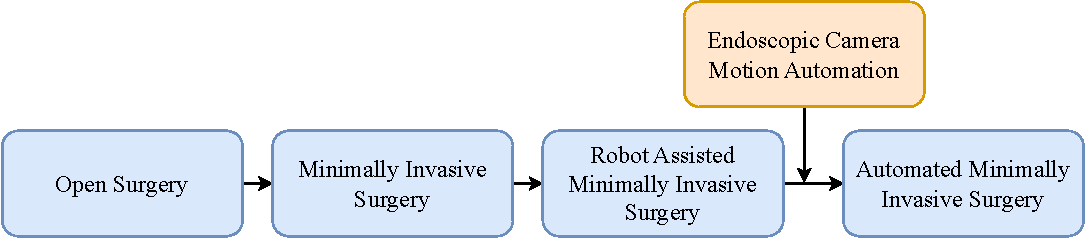
\includegraphics[width=0.9\textwidth]{introduction/fig/24_02_13_surgical_revolution.pdf}
    \caption{The gradual introduction of novel technology into the surgical field, one enabling the next. Endoscopic camera motion automation is likely to appear first towards full automation. Refers to \secref{in:sec:foreword}.}
    \label{in:fig:camera_motion_automation}
\end{figure}

The ever evolving field of surgery has repeatedly demonstrated acceptance of new technology \cite{attanasio2021autonomoy}, and we argue that automation is no exception. The growth of RMIS can clearly be considered an enabling factor for full automation, see also \figref{in:fig:camera_motion_automation}.

When compared to other domains, such as autonomous driving, service and household robots, where robots already exert a significant amount autonomy that far exceeds RMIS, it becomes evident that advances in autonomy will ultimately make their way into the operating theater as well. Regulatory and economic hurdles cause delays in the adoption of novel technology by healthcare systems and hospital units. However, there might even be a future where RMIS will not only adopt full automation from other domains but make significant contributions to general machine intelligence. 

Others \cite{lecun2022path} have argued that machines will need to interact with the real world in order to become truly intelligent and, arguably, RMIS has grown to be the most advanced physical human-robot interaction (pHRI) domain with thousands of deployed robots.
\begin{figure}[t]
    \centering
    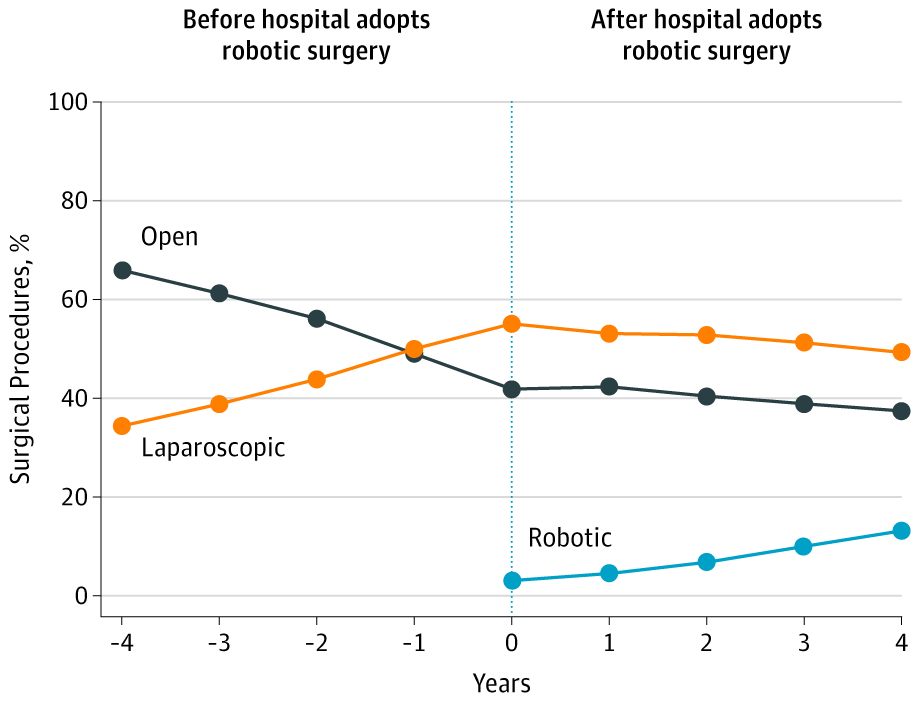
\includegraphics[width=0.6\textwidth]{introduction/img/robotic_since_introduction.png}
    \caption{Increase of laparoscopy over open approaches and robotic laparoscopy versus other methods, respectively. Data normalized to year zero, the introduction of robotic laparoscopy. The use of robotic laparoscopy increased from $1.8\%$ to $15.1\%$. For inguinal hernia repair, an increase in robotic surgery from $0.7\%$ to $28.8\%$ was found. A total of $169.404$ cases over 73 hospitals in Michigan, United States, were investigated. Figure and data provided with courtesy of \cite{sheetz2020trends}. Refers to \secref{in:sec:foreword}.}
    \label{in:fig:robotic_vs_laparoscopic_vs_open}
\end{figure}

As we dive deeper into level five autonomy endoscopic camera motion automation, this introductory chapter will provide a necessary clinical background for laparoscopy in \secref{in:sec:laparoscopy}, a sub-domain of endoscopy, including an in-depth explanation of laparoscopic cholecystectomy (minimally invasive gallbladder removal). Laparoscopic cholecystectomy is the most commonly performed laparoscopic procedure \cite{sheetz2020trends}, and can be considered relatively simple. Therefore, due to vast amounts of readily available data, it serves as the perfect test-bed for the methods that are derived as part of this thesis. 

Next, we explain the rise of robot assisted laparoscopy in \secref{in:sec:robot_assisted_laparoscopy} and the potentials of automation that evolve with it. We highlight different commercial systems, their limitations, and propose innovative solutions. Identified limitations will include spatial awareness, refer \secref{in:sec:spatial_awareness}, as most RMIS systems lack a world model, and, crucially, camera motion automation, for which a thorough review of related methods is provided in \secref{in:sec:camera_motion_automation}. Following the camera motion automation literature review, we will hypothesize an approach to near-term full automation. The proposed approach will revolve around a mixture of imitation learning an classical control. It is grounded in successful automation in related domains and will be discussed in \secref{in:sec:imitation_learning_for_camera_motion_automation}.

\section{Laparoscopy}
\label{in:sec:laparoscopy}
Endoscopy refers to the observation of internal parts by means of an endoscope \cite{oedendoscopy}. The word endoscopy derives from the Greek by combining the prefix "endo" meaning "within" and the verb "skopein", "to view or observe" \cite{majumdar1993short}. In the surgical context, endoscopy refers to a MIS with the goal to observe within the body. Endoscopy inside the abdominal (belly) or pelvic (hip) cavity is called laparoscopy. During laparoscopy, an endoscope, called laparoscope in this clinical context, is inserted through small incisions for diagnostic or interventional purposes, see \figref{in:fig:laparoscopy}.
\begin{figure}[tb]
    \centering
    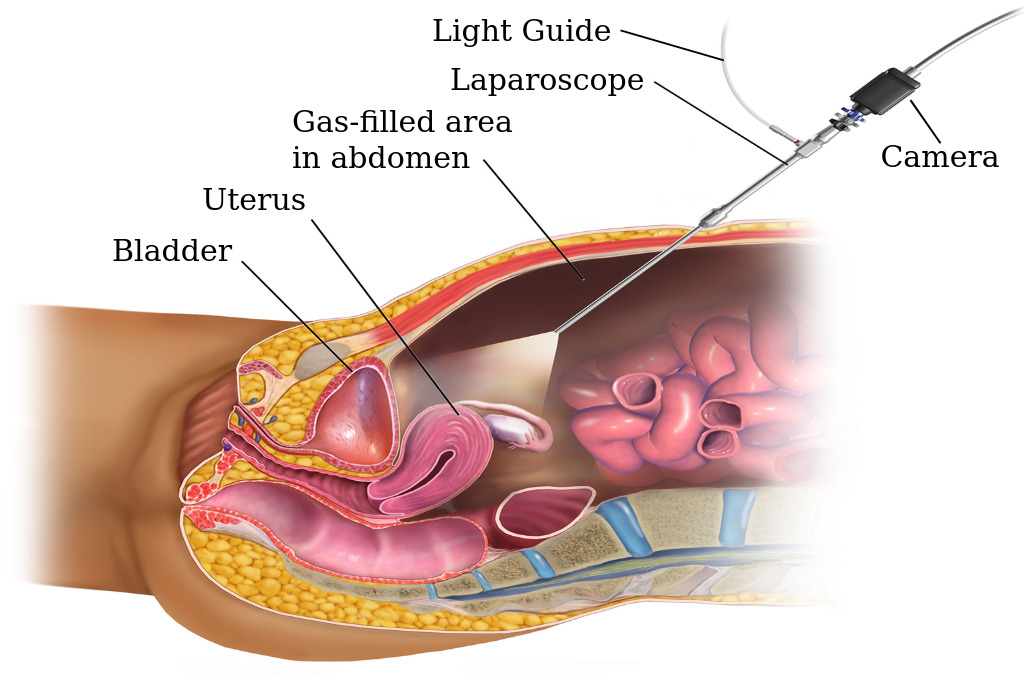
\includegraphics[width=0.7\textwidth]{introduction/img/laparoscopy.jpg}
    \caption{Illustration of a laparoscopic procedure. The laparoscope is inserted through a small incision in the patient's abdominal wall and provides a view of the surgical scene. To provide space, carbon dioxide ($\text{CO}_2$) is injected through a needle into the abdomen. Image provided with courtesy of \cite{blausen2014laparoscopy}. Refers to \secref{in:sec:laparoscopy}.}
    \label{in:fig:laparoscopy}
\end{figure}

Compared to open surgery, laparoscopy leads to significantly faster interventions ($57.19\pm10.13\,\text{min}$ vs. $85.10\pm15.18\,\text{min}$), less bleeding complications ($2\%$ vs $7\%$ of interventions), shorter hospital stays ($2.1\pm1.1\,\text{days}$ vs $4.4\pm2.1\,\text{days}$), less infections, and less post-operative pain \cite{shi2023laparoscopic}. These eminent advantages of laparoscopic over open techniques have led to their adoption since their introduction in the early 1980s, see \figref{in:fig:robotic_vs_laparoscopic_vs_open}. This trend is foreseen to continue and even increase as the majority of surgical residents is nowadays trained on the minimally invasive procedure variants \cite{john2020rise}.

Some types of laparoscopic procedures are cholecystectomy (gallbladder removal), appendectomy (appendix removal), inguinal hernia repair (i.e. leaking of intestines through the abdominal wall), colectomy (partial colon removal), nephrectomy (partial or complete kidney removal), prostatectomy (partial or complete prostate removal), adrenalectomy (removal of the adrenal gland), and gastrectomy (partial or full stomach removal) among others. Since laparoscopic cholecystectomy is carried out in high volumes and is additionally a relatively simple procedure, it is of special relevance to this work. It will thus be considered an example for explaining a laparoscopic surgery setup and procedure.

Cholecystectomy is the surgical removal of the gallbladder. The gallbladder serves as a reservoir for the liver-produced bile, a fat digesting fluid. Bile may harden and form gallstones, which can lead to inflammation and severe pain. Since the liver also releases bile directly into the digestive tract, shown in \figref{in:fig:cholecystectomy_incisions}, the gallbladder may be removed when necessary. A cholecystectomy setup is depicted in \figref{in:fig:room_setup}.
\begin{figure}[tb]
    \centering
    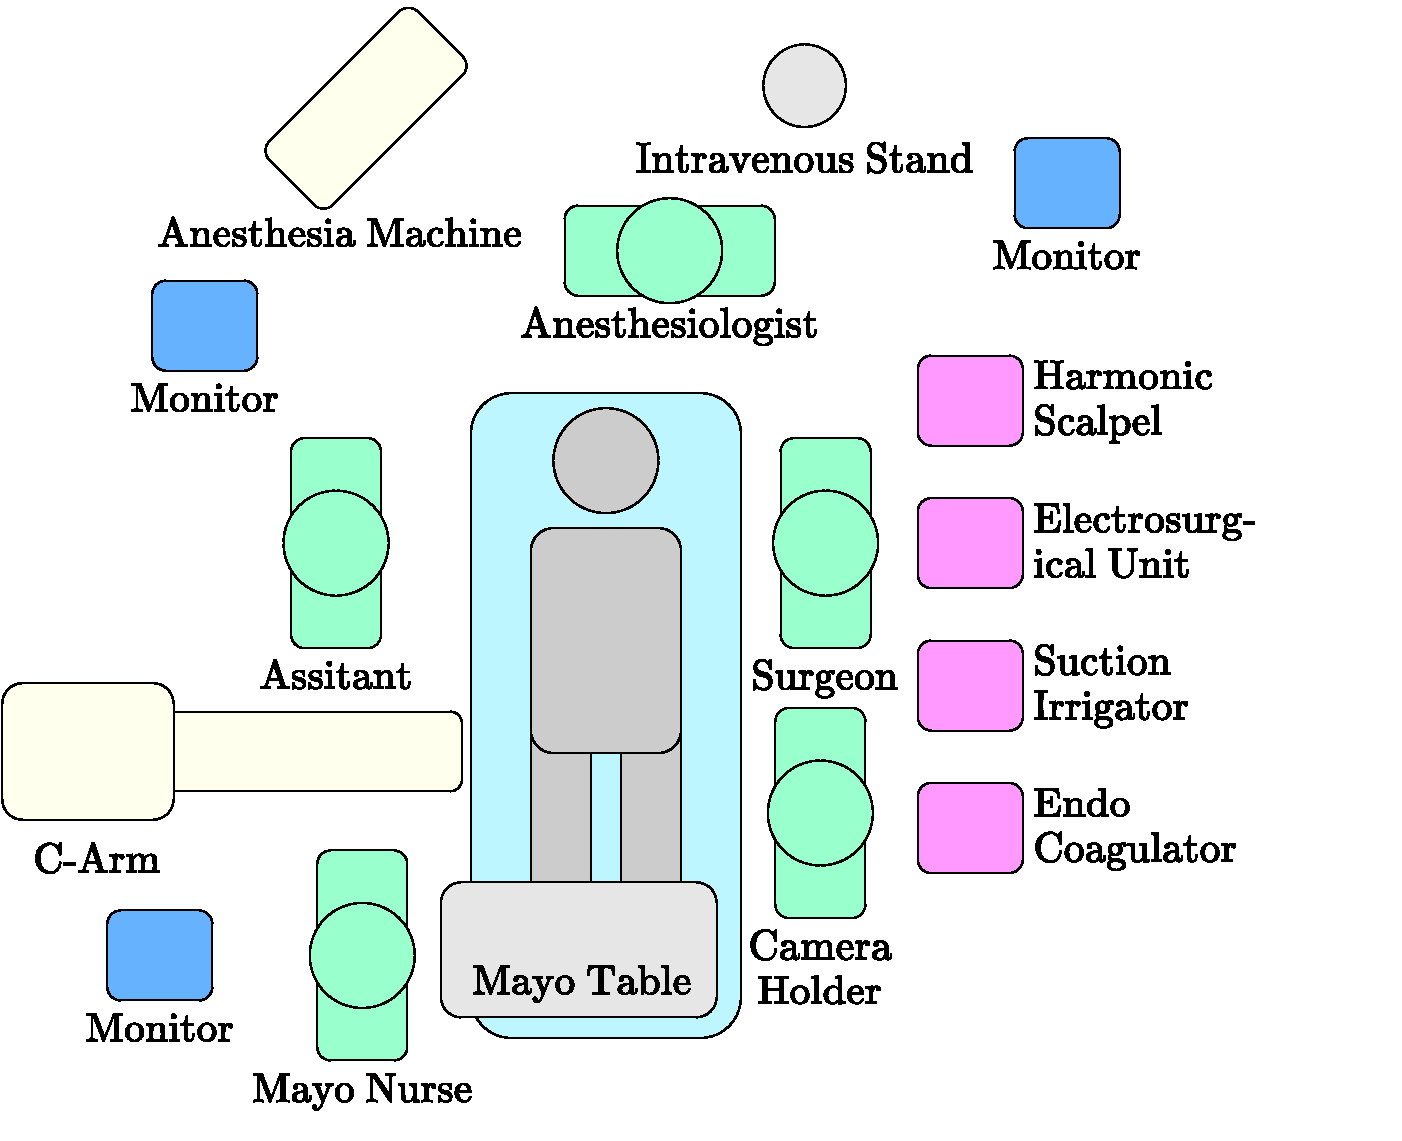
\includegraphics[width=0.7\textwidth]{introduction/fig/24_01_26_room_setup.pdf}
    \caption{Typical setup for a cholecystectomy. Image adapted from \cite{sages2010room}. Refers to \secref{in:sec:cholecystectomy_setup}.}
    \label{in:fig:room_setup}
\end{figure}
\subsection{Laparoscopic Cholecystectomy Setup}
\label{in:sec:cholecystectomy_setup}

Even this relatively simple procedure requires multiple skilled practitioners. The surgeon is supported by an endoscope holder, a second assistant, an anesthesiologist, and a mayo nurse (for providing tools). The procedure commonly requires a harmonic scalpel, which cauterizes tissue and coagulates blood (i.e. causes blood clothing) through ultra-sonic waves. Due to lower cost for cauterization and coagulation, it may be preferable to use an electrosurgical unit (ESU), which generates different electrical waveforms and can be connected to most laparoscopic tools \cite{archana2018comparing}. Further devices include a suction-irrigator for removing body fluids from the surgical scene, as well as an endoscopic camera system, a light source, and multiple monitors. A laparoflator is used to insulflate the abdomen with $\text{CO}_2$ and to maintain a fixed pressure. An anesthesia machine and an intravenous stand are utilized to regulate the patient's conditions. Finally, a C-arm may visualise the bile duct to probe for possible injuries and leakage caused by the intervention \cite{cuschieri1994intraoperative}. The procedure is then referred to as cholangiography (x-ray visualization of the bile duct with contrast agent).

\subsection{Laparoscopic Cholecystectomy Procedure}
\label{in:sec:cholecystectomy_procedure}
\begin{figure}[tb]
    \centering
    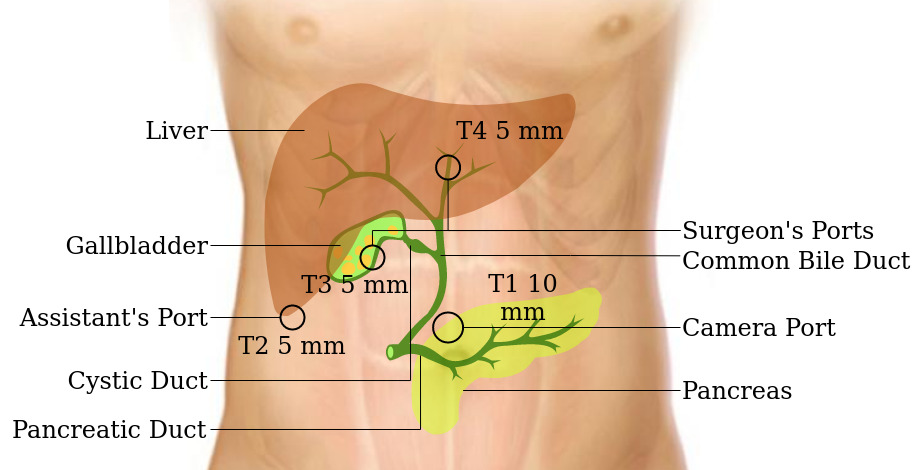
\includegraphics[width=0.9\textwidth]{introduction/fig/24_01_26_cholecystectomy_incisions.jpg}
    \caption{Common cholecystectomy incisions. Several incisions are made for the trocars T1-T4. Image with courtesy of \cite{ALES5766} and modified to include port descriptions and organs. Refers to \secref{in:sec:cholecystectomy_procedure}}
    \label{in:fig:cholecystectomy_incisions}
\end{figure}

This paragraph explains laparoscopic cholecystectomy in simplified terms and vastly refers to \cite{ALES5766}. To begin with, $\text{CO}_2$ is injected into the abdomen via a needle. The pressure is controlled through the laparoflator, see \figref{in:fig:room_setup}. Next, four small incisions are made for trocars T1-T4, which serve as entry point through the abdominal wall, shown in \figref{in:fig:cholecystectomy_incisions}. A laparoscope is inserted through T1 to grant an adequate view of the surgical scene. A grasper is inserted through T2 and used by the assistant to elevate the gallbladder. Trocars T3 and T4 are used by the surgeon to perform the cholecystectomy. It is important to identify anatomical landmarks before other steps are attempted. A good exposure of the surgical area is achieved through adequate patient and port positioning \cite{gupta2023achieve}. Following the preparatory steps, the surgery can broadly be partitioned into six steps. These steps will be explained in the following.

\subsubsection{Step 1: Dissection of the Hepatocystic Triangle}
The goal is to expose the hepatocystic trianlge \cite{mischinger2020critical}, see \figref{in:fig:hepatocystic_triangle}. The gallbladder is gently pulled upward over the liver and its neck is pulled downward to expose its different parts, as can be seen in \figref{in:fig:cholecystectomy_incisions}. Swollen gallbladders are precautiously decompressed with a needle to prevent perforation with leakage of bile and gallstones. Potential adhesions (scarred connections to other organs) are carefully separated using cautery and regular tools, avoiding the area near the duodenum (beginning of the small intestine). Next, the hepatocystic triangle is dissected by carefully removing fibrous and fatty tissue. It is of utmost importance that no tubular structure may be damaged until cystic duct and cystic artery are identified \cite{mischinger2020critical}.
\begin{figure}[tb]
    \centering
    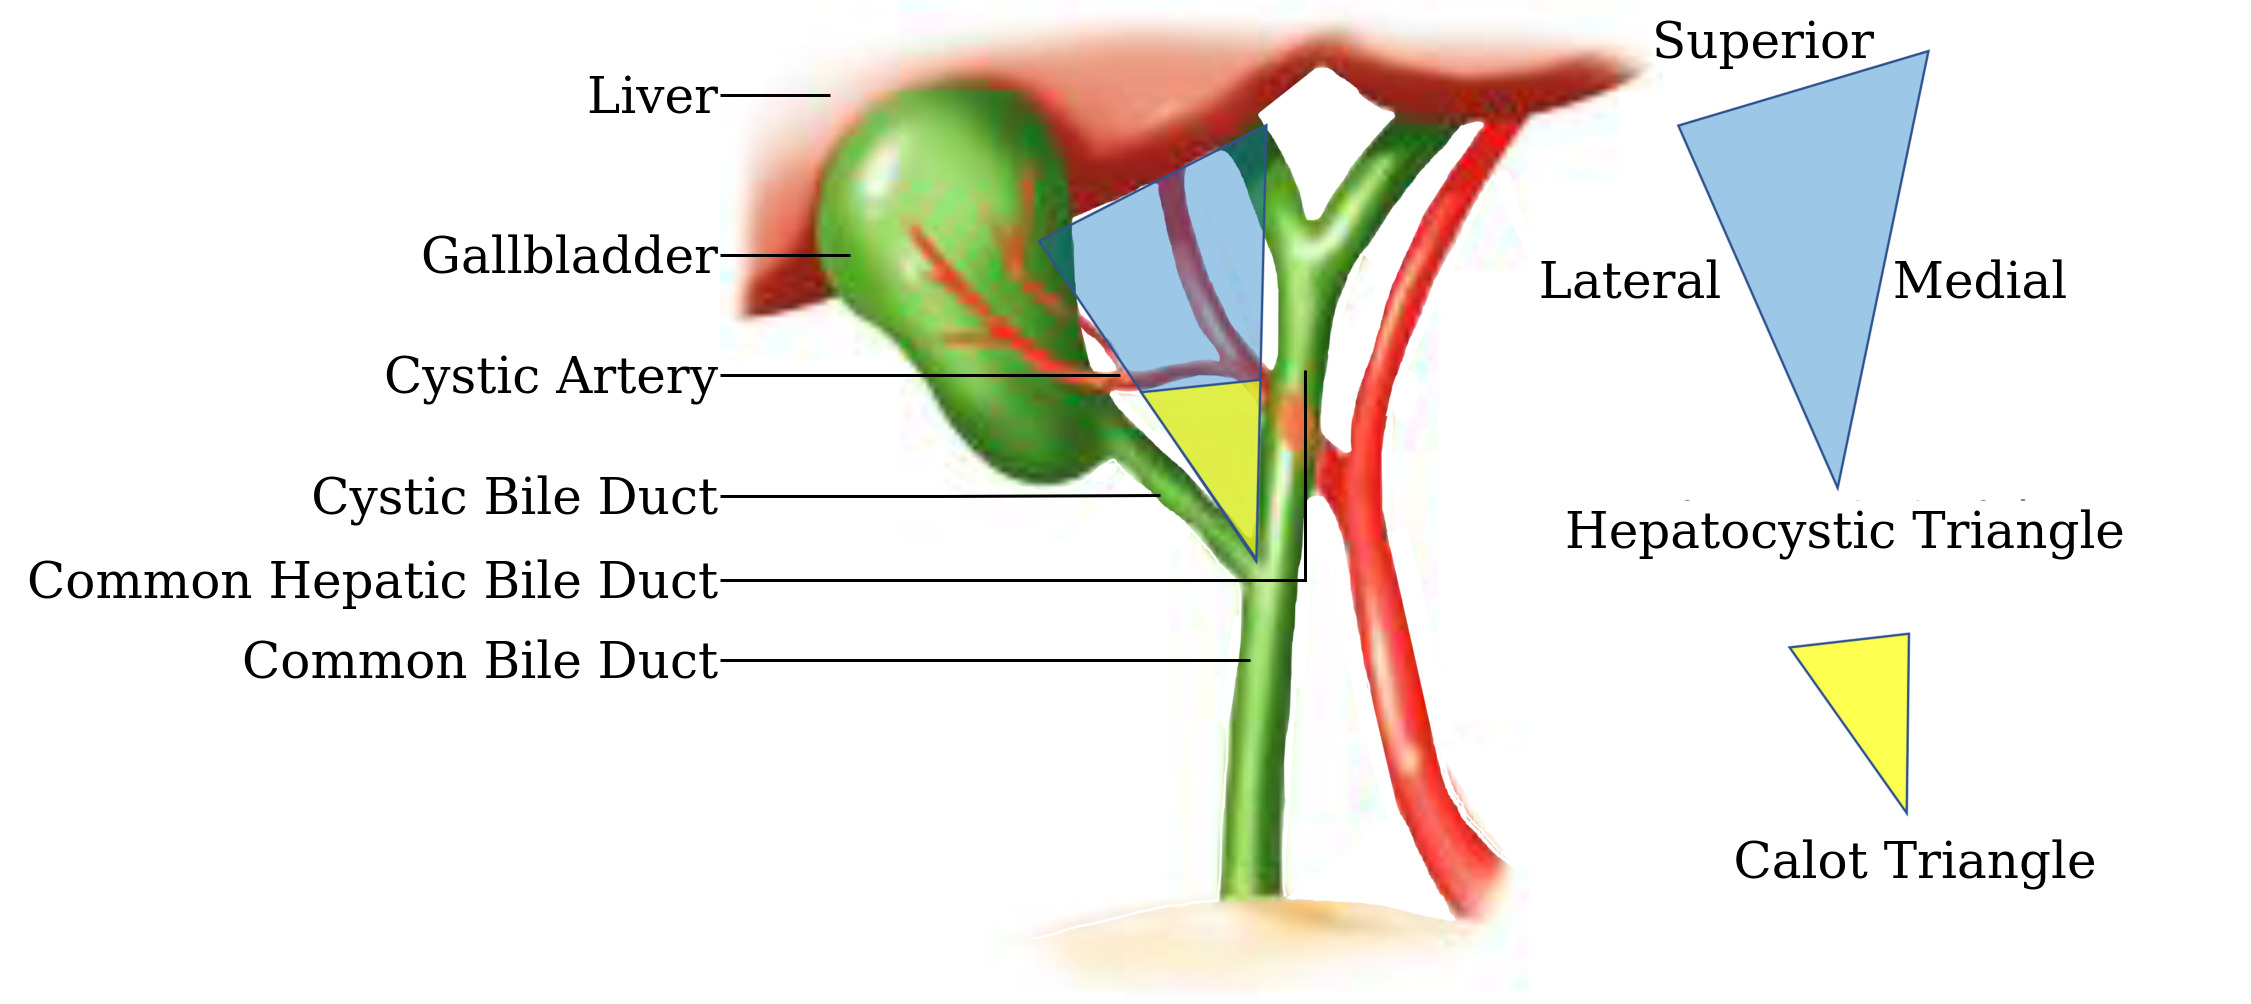
\includegraphics[width=0.8\textwidth]{introduction/fig/24_02_03_hepatocystic_triangle.jpg}
    \caption{The bile duct (green), together with liver and gallbladder form the hepatocystic triangle, which is often covered in fat tissue. Image with courtesy of \cite{mischinger2020critical} and updated font. Refers to \secref{in:sec:cholecystectomy_procedure}.}
    \label{in:fig:hepatocystic_triangle}
\end{figure}

\subsubsection{Step 2: Establishing the Critical View of Safety} 
\label{in:sec:critical_view_of_safety}
The critical view of safety defines a state that is achieved through the hepatocystic triangle dissection, it is shown in \figref{in:sec:cholecystectomy_procedure}. No tubular structure may be damaged prior to achieving the critical view of safety. The critical view of safety is defined by three conditions. First, the hepatocystic triangle is cleared of all fat and fibrous tissue. The common bile duct and the common hepatic bile duct are identified but not exposed. Second, the lower third of the gallbladder is separated from the liver. Third, only two structures are identified entering the gallbladder, the cystic duct and the cystic artery. The surgery is halted in this stage and reflected upon. Potential anatomical variations are discussed.

\begin{figure}[tb]
    \centering
    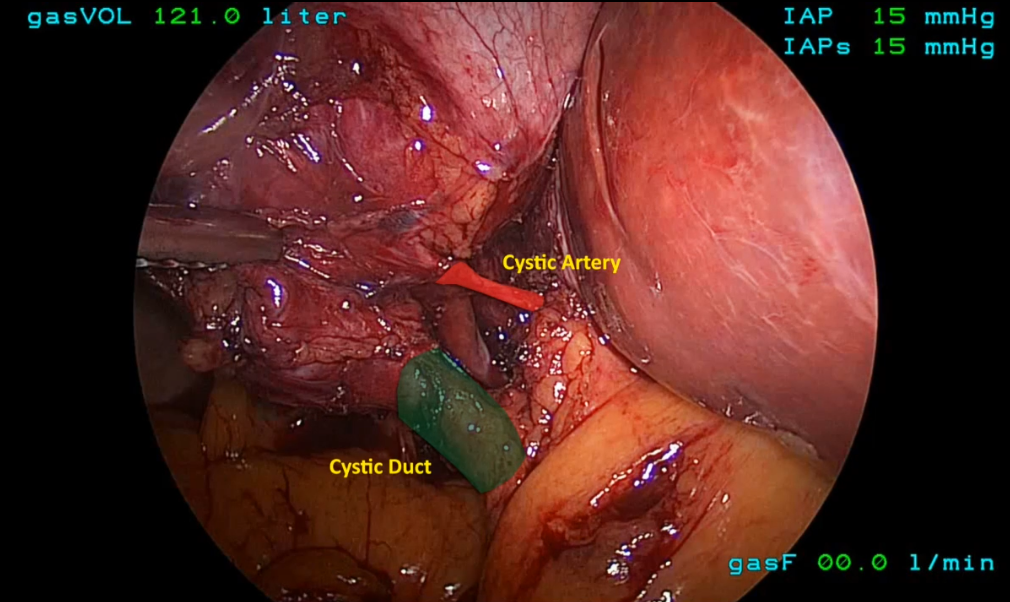
\includegraphics[width=0.6\textwidth]{introduction/img/critical_view_of_safety.png}
    \caption{The critical view of safety. The cystic artery is indicated in red, the cystic duct in green. Image provided with courtesy of \cite{ALES5766}. Refers to \secref{in:sec:cholecystectomy_procedure}.}
    \label{fig:enter-label}
\end{figure}

\subsubsection{Step 3: Clipping and Cutting the Cystic Artery} After establishing the critical view of safety, the next step is to separate the gallbladder from the cystic artery. Therefore, the csytic artery is clipped twice proximally (i.e. the side of the artery that stays inside the body) and once distally (i.e. on the side of the to be removed gallbladder). The distal clip should be attached close to the neck of the gallbladder to leave sufficient space for cutting. Next, the artery is cut with hook scissors, leaving some space at the proximal end to prevent the clip from detaching.

\subsubsection{Step 4: Operative Cholangiography and Cutting the Cystic Duct} Post cutting the cystic artery, it is sometimes preferred to perform cholangiography, using the C-arm X-ray, which is shown in \figref{in:fig:room_setup}. This is to verify a functioning bile tree. First, the cystic duct is clipped distally, and then incised partially with hook scissors. Next, the common bile duct is flushed with saline and a contrast agent is injected. Fluoroscopy should reveal free flow of the contrast agent into the common hepactic bile duct, its left and right branches into the liver, as well as free flow into the duodenum via the common bile duct. Once satisfactory flow is observed, the cystic duct is clipped proximally and cut as the cystic artery in step three.

% also refer to \secref{in:sec:cholecystectomy_setup}
% ERCP: https://www.sages.org/publications/patient-information/patient-information-for-ercp-endoscopic-retrograde-cholangio-pancreatography-from-sages/

\subsubsection{Step 5: Separating Gallbladder from Liver} After cutting the cystic duct, the gallbladder is carefully dissected from the liver bed, commonly using an L-hook with monopolar energy. Care must be taken to prevent liver bed injury as this may cause bleeding and or bile leakage from superficial ducts. Entry into the gallbladder should be avoided as this may cause bile and bile stone leakage, which, however, can be removed with a suction irrigator, as shown in \figref{in:sec:cholecystectomy_setup}. In complex conditions with gallbladder inflammation, an ultrasound-driven harmonic scalpel may be used to perform ultrasonic coagulation to maintain hemostasis (blood thickening). Finally, the liver bed is once more inspected before separating the gallbladder fully. The surgical side is once more irrigated and cleaned of any blood and bile. The gallbladder is then put into a specimen bag.

\subsubsection{Step 6: Removing Specimen and Closing} Once in a bag, the gallbladder is removed through the T1 port, refer to \figref{in:fig:cholecystectomy_incisions}. This may require widening of the opening in the presence of larger stones. The ports T1-T4 are being vented to remove residual $\text{CO}_2$. Following that, the skin and fascia at the extraction site are closed with sutures.

\section{Robot Assisted Laparoscopy}
\label{in:sec:robot_assisted_laparoscopy}
Having a good understanding of laparoscopic surgery from the previous \secref{in:sec:laparoscopy}, and more specifically, laparoscopic cholecystectomy, we will next discuss robot assisted laparoscopic surgery. We will initially explain the, at first glance, paradoxical rise of robot assisted laparoscopy in \secref{in:sec:the_rise_of_robot_assisted_laparoscopy}. Next, current commercial systems will be analyzed in \secref{in:sec:robot_surgery_platforms}, as to better understand where the field might be headed so to provide an informed research direction. Finally, based on the knowledge of the previous sections, the enhancement of current systems will be discussed in \secref{in:sec:enhancing_current_systems}.

\subsection{The Rise of Robot Assisted Laparoscopy}
\label{in:sec:the_rise_of_robot_assisted_laparoscopy}
According to many, the future of surgery is robotic \cite{times2021better}. This trend was already exposed in \secref{in:sec:foreword}, \figref{in:fig:robotic_vs_laparoscopic_vs_open}, where \cite{sheetz2020trends} found an average increase in robotic laparoscopy from $1.8\%$ to $15.1\%$ post robotic laparoscopy introduction. For cholecystectomy, the most common procedure, an increase from $2.5\%$ to $7.5\%$ was found. Somewhat paradoxically, laparoscopic cholecystectomy is already a routine procedure with very low complication rates, \cite{thapar2023evaluation} e.g. reports a $0.2\%$ 30 days mortality rate in India. Hence, questions about benefits of robotic laparoscopy may rightfully be raised.

\paragraph{Patient Side Aspects} More than twenty years have passed since the introduction of the da Vinci\textsuperscript{\textregistered} surgical robot by Intuitive (\figref{in:fig:da_vinci}), which was launched in 1999, and many review studies compared classical vs. robotic laparoscopies ever since to provide evidence-based care. The majority of studies suggests that no significant advantages exist for patients. Despite increased cost and longer intervention times, these studies report equal complication, mortality, and conversion rates (i.e. conversion to open surgery), as well as equal post operative stay duration \cite{kawka2023laparoscopic, csirzo2023robot}. Some studies, however, also highlight underrepresented patient-reported outcome measures \cite{kawka2023laparoscopic} (e.g. post-operative pain, return to function). 

\paragraph{Surgeon Side Aspects} Undoubtedly, the market for RAS, which is currently dominated by Intuitive Surgical, Inc., is sustainably growing. 

%, see \figref{in:fig:intuitive_revenue}.
\begin{figure}[tb]
    \centering
    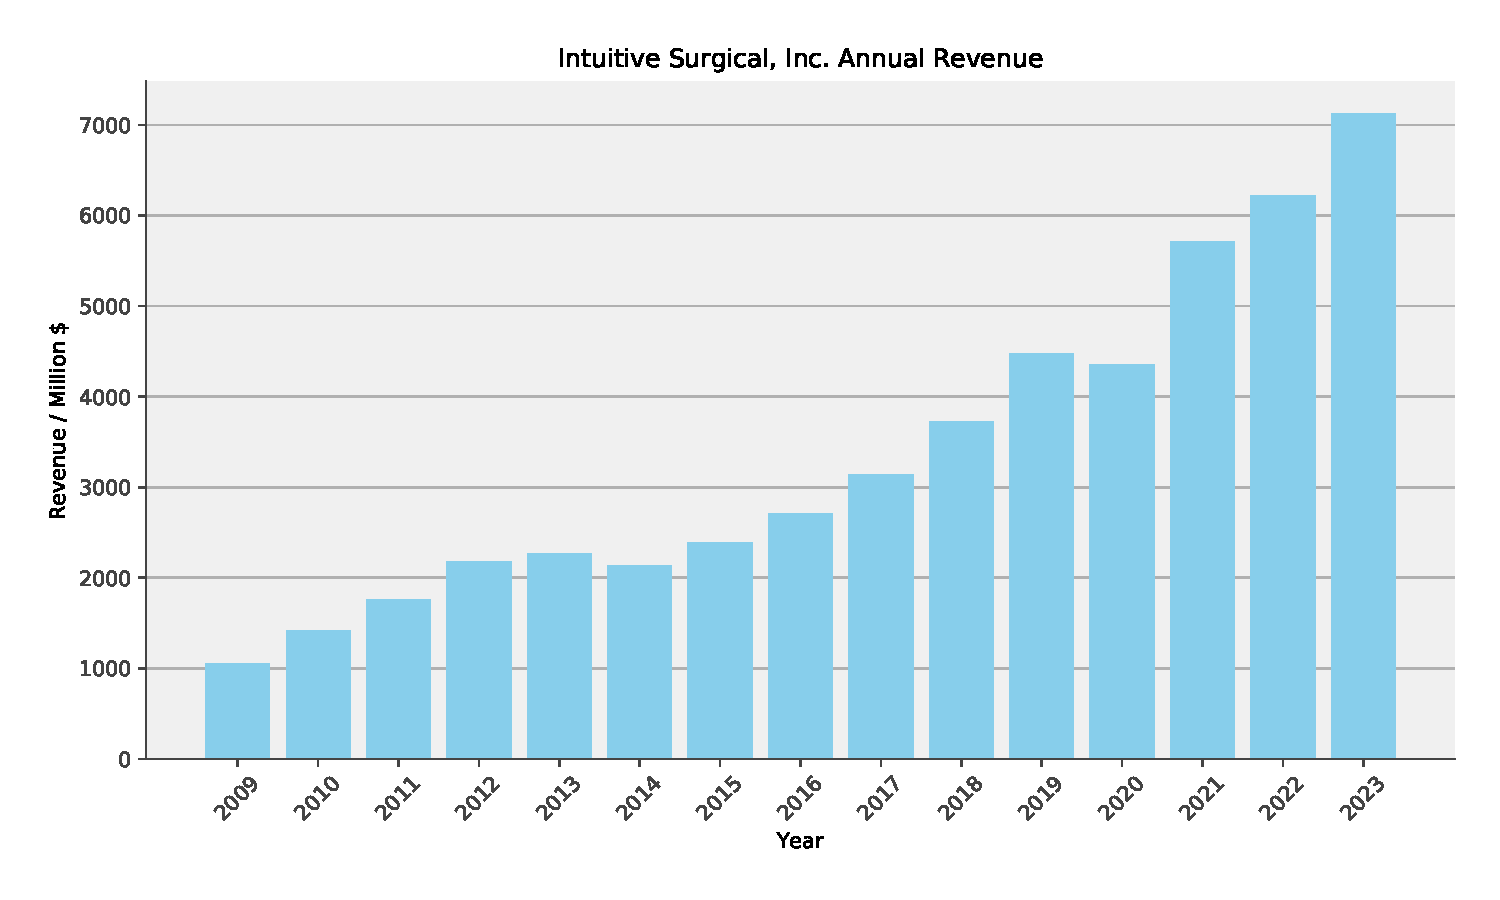
\includegraphics[width=0.9\textwidth]{introduction/fig/intuitive_revenue.pdf}
    \caption{Annual revenue of Intuitive Surgical, Inc. from 2009 to 2023. The company has achieved sustained growth throughout the years. Data obtained from \cite{intuitiverevenue}.}
    \label{in:fig:intuitive_revenue}
\end{figure}

The reasons for this steady growth, as per above and to the best current knowledge, cannot be associated with patient benefits. Instead, the growth can be linked to surgeon benefits. Multiple studies suggest ergonomic advantages for surgeons \cite{monfared2022comparison, zarate2019ergonomic}, which prevent operating burnout \cite{wells2019operating} and improve longevity \cite{stucky2018surgeon}. This evidence can best be understood through the surgery that lead to the initial success of the da Vinci\textsuperscript{\textregistered} surgical robot, the minimally invasive prostatectomy. The prostate, being located low (inferiorly) in the pelvis, is hardly accessible via laparoscopic tools. The large distance from trocar to prostate makes precise motion difficult and creates a lever that generates torques which cause fatigue. A robot makes it ergonomically much simpler to operate in these areas. In England, about $85\%$ of radical prostatectomies in $2017$ were performed robotically \cite{maynou2021patterns}.

\paragraph{Interviewing a Surgeon} To find further qualitative insights on the advantages of RMIS over MIS, we interviewed Nicholas Raison, a consultant urological surgeon, during a course he organized for robotic partial nephrectomy, hosted by the International Medical Robotics Academy at Guy's Hospital King's College London. Among the aforementioned lever with associated fatigue reduction, and precision improvements, he named four more advantages of robotic platforms. First, classical laparoscopic tools are straight and do not allow for wrist rotations at the grippers. Robotic tools provide additional degrees of freedom and therefore increased dexterity. This simplifies tasks such as suturing significantly. Second, the control of the tools through a console allows the surgeon to operate from a first-person view which reduces mental burden. Third, RMIS reduces the learning curve for newly trained surgeons, which results from the enhanced dexterity and the first-person view.
Finally, since surgeons are in charge of moving the camera themselves in RMIS, they tend to move it more frequently which provides them with a precise view. In classical MIS, there exists a communication barrier with the camera holder, refer \figref{in:fig:room_setup}. Therefore, in classical MIS, camera holders sometimes show a distant view to compensate for this communication barrier. This last point highlights the potential value of endoscope motion automation, enabling a future fusion of RMIS and MIS techniques. 

\paragraph{Future Aspects} In summary, and to best current evidence, robotic surgery platforms currently do not provide  improved surgery outcomes, but increase operating cost and time. Viewed differently, they don't worsen the surgery outcomes either. What makes robotic laparoscopy so successful are the surgeon side benefits and its future prospects. These e.g. include the possibility to control the systems remotely, data collection, realistic simulations for training, and potential automation. With this in mind, the research carried out in this thesis aims to address the increased cost and  time components, emphasizing on laparoscopic camera motion automation. To get a better understanding for how this could best be achieved, the next section provides an overview of current robot surgery platforms.

% ⁃	Versius jerky, less smooth, no rotation about entry axis
% ⁃	Hugo better range of motion inside abdomen vs xi
% ⁃	Xi console restricting (goggles)
% ⁃	Hugo console open 
% ⁃	Versius console no foot pedals 
% ⁃	Versius common laparoscopic tools, cheaper but less versatile
% ⁃	Much more camera motion in robotic surgery compared to classic laparoscopic surgery (surgeons adjust to their desired view more commonly. Camera in traditional surgery further away to correct for communication shortcoming)
% ⁃	Ergonomic benefits in robotic surgery (large lever over entry point, generating lots of torque)
% ⁃	Versius small company in comparison to pharmaceutical giants 
% ⁃	Footprint xi surprisingly small 
% ⁃	Da Vinci console weight engaged, Hugo head tracking engaged (tracks glasses via camera and infrared balls on glasses)
% ⁃	Hugo console feels laggy compared to da Vinci 
% ⁃	Classical laparoscopic tools are straight, robotic tools offer additional dof, making e.g. suturing much simpler
% ⁃	Da Vinci arm arm collisions happen, in which case the assistant attempts to readjust the configuration 
% ⁃	Versius changes tools via joystick, whereas other systems can change arm via footpedals
% ⁃	Proximie providing views of the da Vinci during live stream 

\subsection{Robot Surgery Platforms}
\label{in:sec:robot_surgery_platforms}
\begin{figure}[tb]
    \centering
    \begin{subfigure}[b]{0.49\textwidth}
        \centering
        \includegraphics[width=\textwidth]{introduction/img/JPG_Large-DV_SYS_Xi_PatientCart_PRF_RGB-min.jpg}
        \caption{The da Vinci\textsuperscript{\textregistered} Xi system. Images provided with courtesy of \textcopyright2023 Intuitive Surgical Operations, Inc.}
        \label{in:fig:da_vinci}
    \end{subfigure}
    \begin{subfigure}[b]{0.49\textwidth}
        \centering
        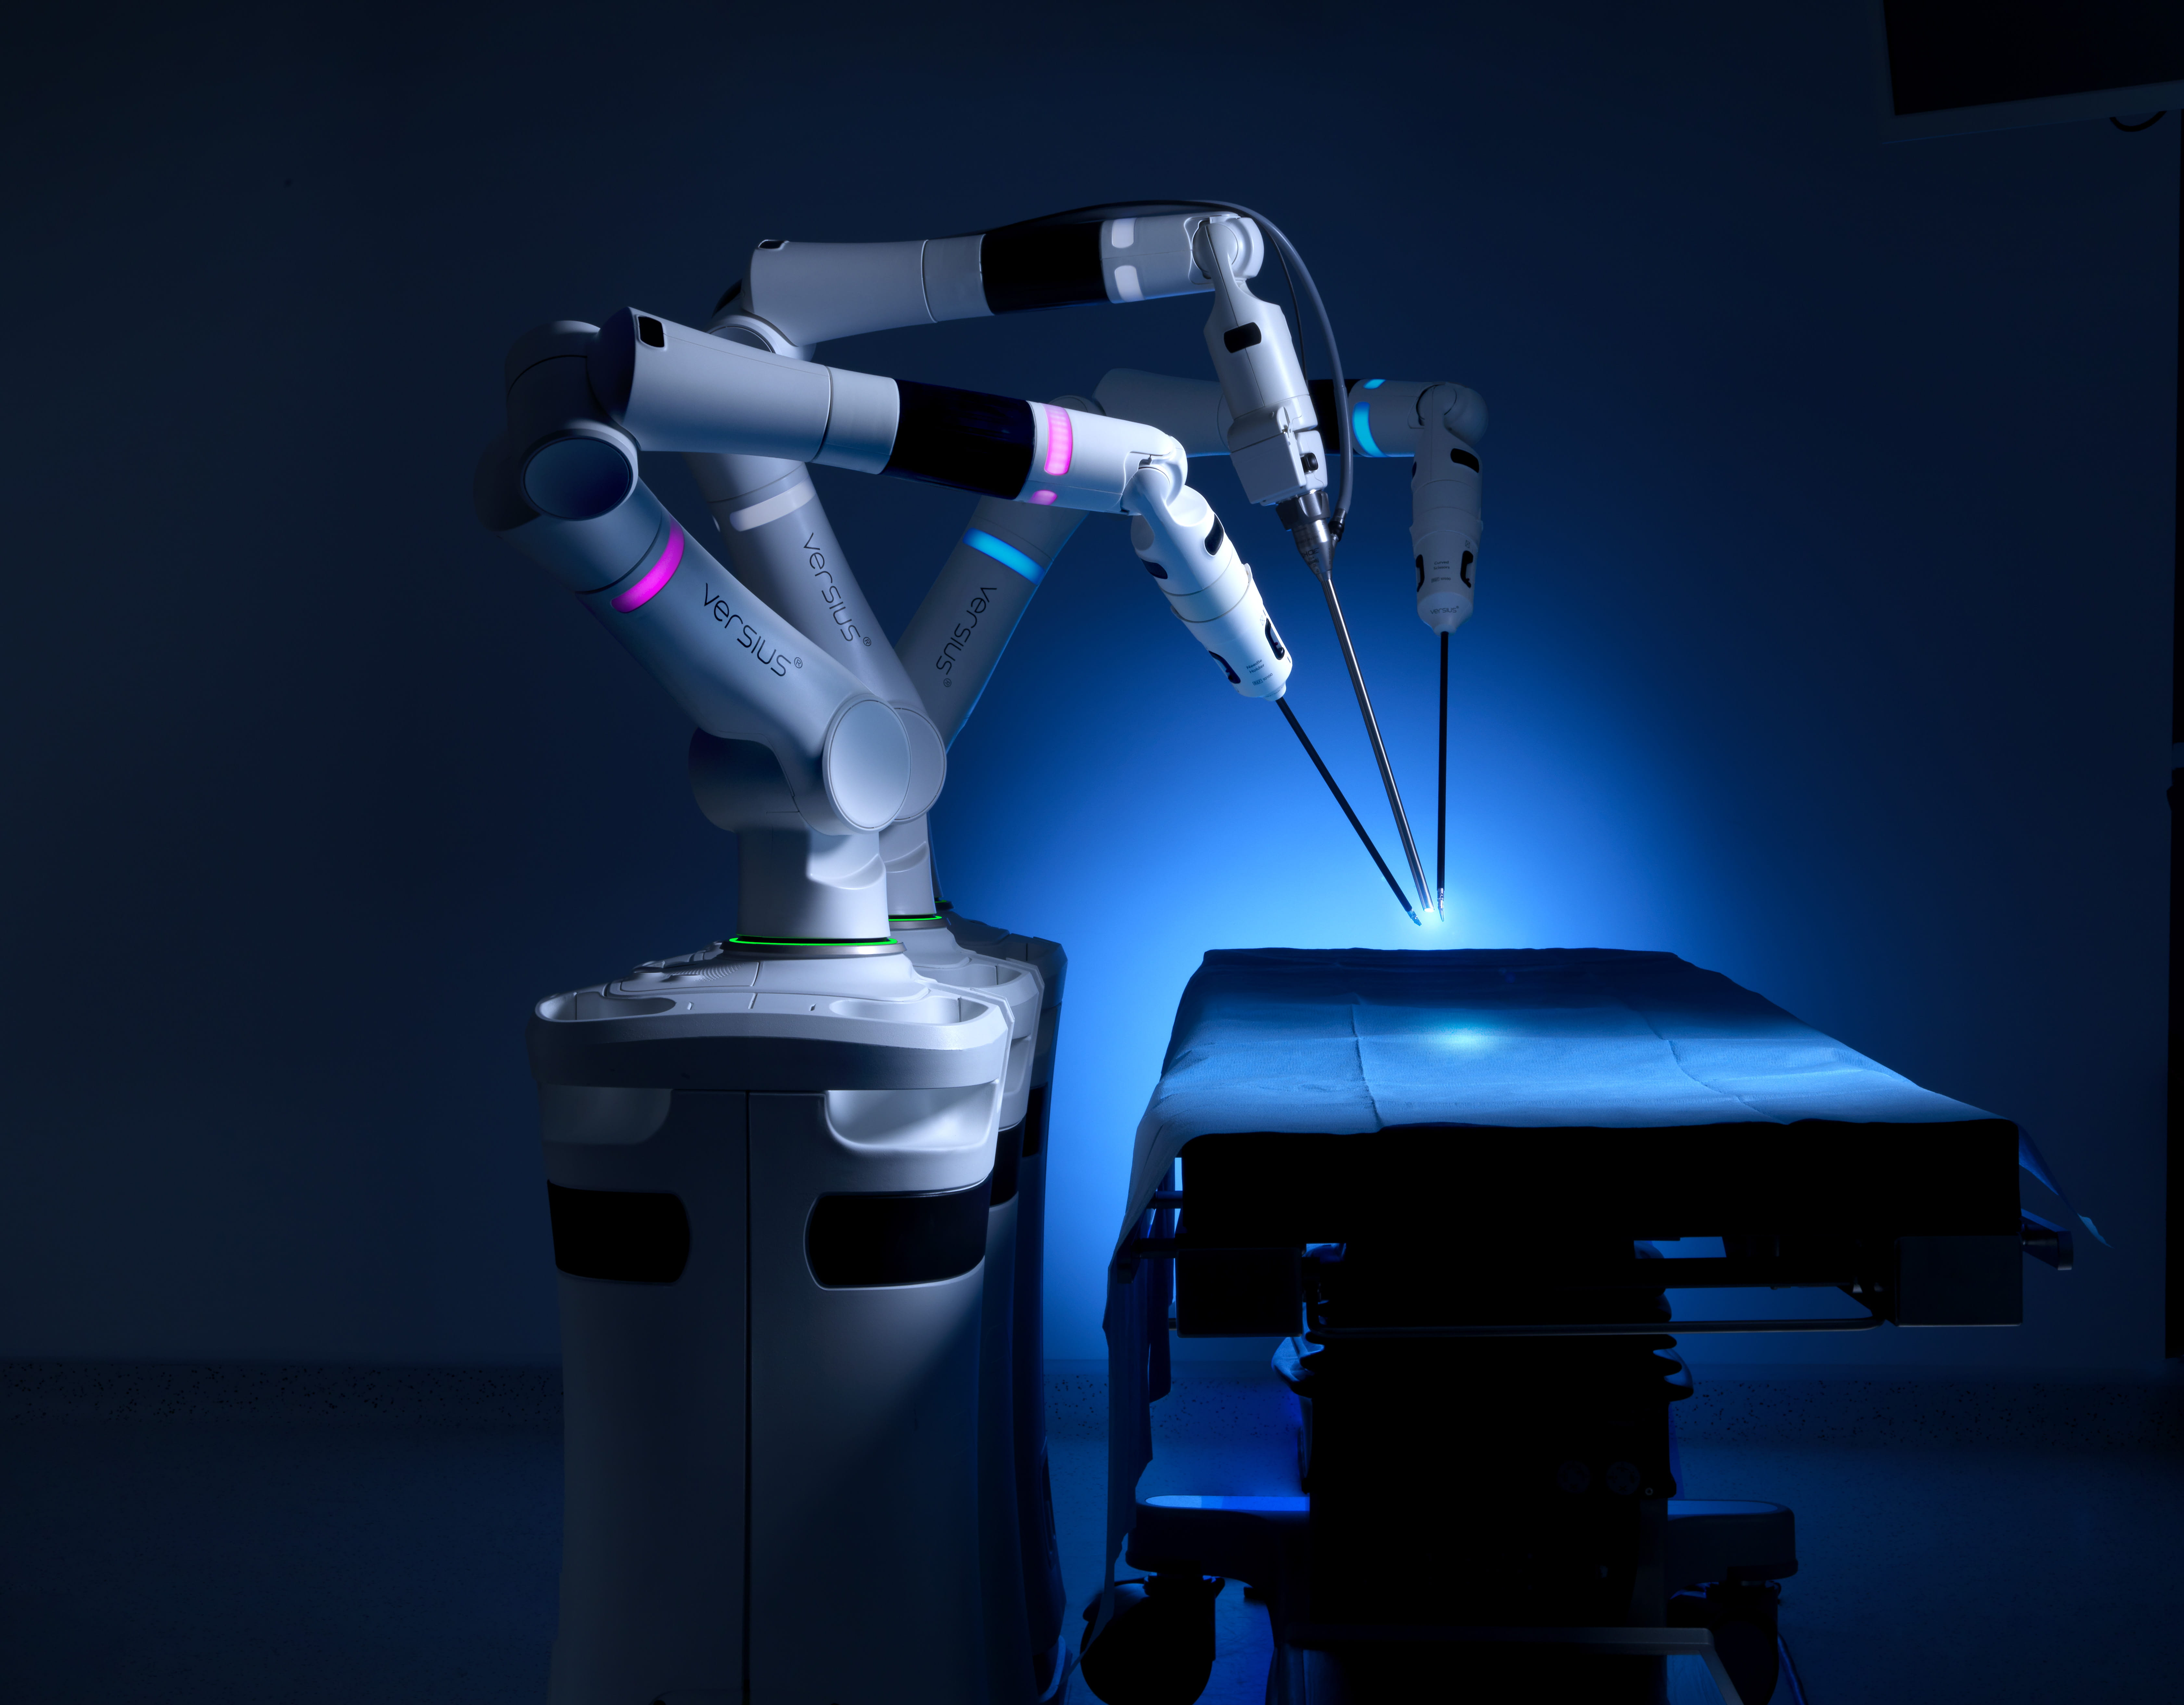
\includegraphics[width=\textwidth]{introduction/img/Product-Versius-3-Arm-Setup-B.jpg}
        \caption{The Versius\textsuperscript{\textregistered} system. Images provided with courtesy of \textcopyright2023 CMR Surgical, Ltd.}
        \label{in:fig:versius}
    \end{subfigure}
    \caption{Two examples of currently available commercial robotic laparoscopy systems. It is demonstrated how competition has led to two very different designs. The da Vinci\textsuperscript{\textregistered} Xi system in \figref{in:fig:da_vinci} is monolithic with a mechanical RCM. The Versius\textsuperscript{\textregistered} system is modular with a programmable RCM. Refers to \secref{in:sec:robot_surgery_platforms}.}
    \label{in:fig:surgical_systems}
\end{figure}

The da Vinci\textsuperscript{\textregistered} robot by Intuitive (\figref{in:fig:da_vinci}) was launched in 1999 by Intuitive Surgical, Inc., which filed multiple patents in the 1990s thereby guarding market access from other companies. Patents in the US generally last for 20 years, which is why as of 2020 most of these critical patents have ran out. Many other companies are now trying to gain some of Intuitive's market share. This competition will ultimately benefit patients, as it might help drive down cost for robotic surgery in the future \cite{patel2021can}, increase accessibility, and lead to innovation in general. 

A non-exhaustive overview of current commercial systems is given in \tabref{in:fig:systems}. It can be seen that the competition has already brought innovation and a broader variety of systems. Multiple companies are adopting Intuitive's monolithic structure, that is all robotic arms are attached to a single instance. Many others, such as Medtronic and CMR Surgical, are taking a modular approach instead. CMR systems further differentiate themselves not only by their modularity, but also through their mechanical properties. The da Vinci\textsuperscript{\textregistered} robot has a mechanical remote center of motion (RCM), i.e. there are dedicated degrees of freedom (DOF) for achieving a zero translational velocity at the entry point to the patient. The RCM is also sometimes called fulcrum point in the medical context. Having a mechanical RCM provides additional safety, but leads to systems that are hard to re-purpose. This is why recent systems are exploring programmable RCMs, in which a RCM is achieved through control theory. This has implications on safety, as sometimes the RCM may not be achieved, but can potentially provide multi-purpose systems. 

\begin{table}[tb]
\centering
\caption{A non-exhaustive list of commercial robotic laparoscopy systems. The table differentiates between monolithic / modular systems and systems with mechanical / programmable remote center of motion (RCM). The market competition has lead to a variety of systems with a tendency to stand apart from Intuitive's status-quo approach. Refers to \secref{in:sec:robot_surgery_platforms}.}
\label{in:fig:systems}
\begin{tabular}{lll}
                                       & Mechanical RCM                                                                                                                                                                                                                                                                                                             & Programmable RCM                                                                                                                                                                                                                                                                                                         \\ \cline{2-3} 
\multicolumn{1}{l|}{Monolithic} & \multicolumn{1}{l|}{\begin{tabular}[c]{@{}l@{}}$\bullet$ da Vinci\textsuperscript{\textregistered} (Intuitive)\\ $\bullet$ Maestro\textsuperscript{\textregistered} (Moon Surgical)\end{tabular}} & \multicolumn{1}{l|}{\begin{tabular}[c]{@{}l@{}}$\bullet$ hinotori\textsuperscript{\texttrademark} (Medicaroid)\\ $\,$\end{tabular}}                                                                                                                                                            \\ \cline{2-3} 
\multicolumn{1}{l|}{Modular}    & \multicolumn{1}{l|}{\begin{tabular}[c]{@{}l@{}}$\bullet$ Hugo\textsuperscript{\texttrademark} (Medtronic)\\ $\bullet$ SSi Mantra\textsuperscript{\texttrademark} (SS Innovations)\\ $\,$\end{tabular}}                                                                                  & \multicolumn{1}{l|}{\begin{tabular}[c]{@{}l@{}}$\bullet$ Versius\textsuperscript{\textregistered} (CMR Surgical)\\ $\bullet$ Dexter\textsuperscript{\textregistered} (Distalmotion)\\ $\bullet$ Senhance\textsuperscript{\texttrademark} (Asensus Surgical)\end{tabular}} \\ \cline{2-3} 
\end{tabular}
\end{table}

\subsection{Enhancing Current Systems}
\label{in:sec:enhancing_current_systems}
The previous two sections gave an explanation for the rise of robot assisted laparoscopy in \secref{in:sec:the_rise_of_robot_assisted_laparoscopy}, and introduced different commercial systems in \secref{in:sec:robot_surgery_platforms}. We identified surgeon side benefits as well as future prospects as the main driving factors for RMIS. Adoption is, however, slowed down by roadblocks such as surgery cost, about $\$1000-4000$ of additional cost per procedure \cite{neumann2018qalys}, and additional operation time, about $25$ minutes of additional operation time for cholecystectomy (185 vs 160 minutes \cite{kane2020robotic}). Patient outcomes are just as good in RMIS as they are in MIS. This is to be expected as patient outcomes for MIS are already much better than for open surgery and the bar for further improvement is high. Consequentially, patient outcomes cannot be considered a limitation of current systems and are thus not of immediate relevance for research. Now, to enhance current systems, we argue that it is most efficient to work on the driving factors that made RMIS successful in the first place, as well as the roadblocks. The overarching goal of this thesis, laparoscopic camera motion automation, fits nicely into the clinically relevant enablers and challenges for RMIS, as shown in \figref{in:fig:advancing_robotic_laparoscopy}. A prerequisite for automating a robotic system in a pHRI environment, however, is spatial awareness. Spatial awareness comes with the additional benefit that it also contributes to operation time and surgeon convenience, as will be described in the next section.
\begin{figure}[tb]
    \centering
    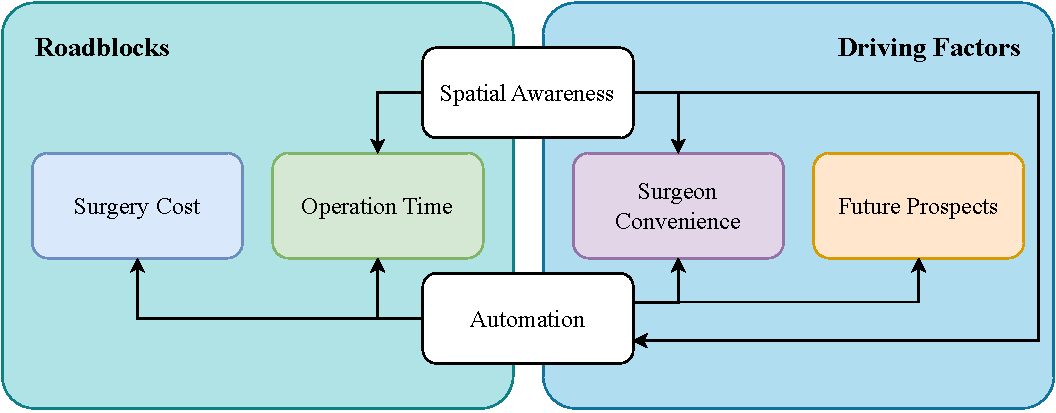
\includegraphics[width=\textwidth]{introduction/fig/main_goals.pdf}
    \caption{Roadblocks and driving factors of RMIS and how the targets of this thesis, spatial awareness and automation, alleviate and enhance them, respectively, refers to \secref{in:sec:enhancing_current_systems}.}
    \label{in:fig:advancing_robotic_laparoscopy}
\end{figure}

\subsubsection{Spatial Awareness}
\label{in:sec:spatial_awareness}
Spatial awareness is likely the most underexplored domain in RMIS. By spatial awareness we will be referring to highly precise localization necessary for surgery, that is in the order of $1\,\text{cm}$ or less. In the cluttered operating theater, containing an anesthesia machine, monitors, a C-arm, staff, the patient, the surgeon, and many other devices, refer \figref{in:fig:room_setup}, collisions are inevitable. A staggering amount of 5 arm-arm, and or assistant-arm collisions occur on average in robotic colorectal surgery \cite{wong2023improving}. Pain or bruising from hindrance by the robot arm is reported by $20\%$ of assistants  \cite{van2019ergonomic}. Training assistants could mitigate some of these issues, which, as many studies imply \cite{cimen2019does, mitsinikos2017does, kwon2020impact}, would lead to improved performance, and therefore, surgeon convenience and operation time reduction. 

To this end, we argue differently and assign the responsibility to the robotic system rather than the assistants or surgeons. These highly capable robotic systems should prevent collisions themselves and leave the clinical workflow unaltered. Some works suggest image-based avoidance \cite{hameed2016towards} and 3D avoidance \cite{li2023three}, both of which could benefit from spatial awareness. Collision avoidance might even become more relevant with the adoption of modular systems, as outlined in \secref{in:sec:robot_surgery_platforms}. Spatial awareness would not only improve performance by reducing collisions, it would further contribute to workspace optimization works, such as \cite{hutzl2015knowledge, zelechowski2023automatic}, as these require accurate knowledge about the relative patient-robot position. Workspace optimization is not only crucial from a robotic point of view but for clinical aspects as well \cite{alhusseinawi2023validation}. As such, recent studies highlight that it takes an average of $18$ minutes to perform proper docking in robotic adrenalectomy \cite{feng2020robot}.

\subsubsection{Automation}
\label{in:sec:automation}
As already outlined in the foreword \secref{in:sec:foreword}, laparoscopic camera motion automation is likely the first milestone towards automated RMIS. The short-term benefits are less obvious than for improved spatial awareness, as discussed above, however, it is an achievable starting point and a foundational building block to delivery long-term benefits. As such, automation, shown in \figref{in:fig:advancing_robotic_laparoscopy}, could have positive implications on surgery cost, operation time, and surgeon convenience.

Some works argue that automation may reduce human error that is linked to fatigue, lack of attention and cognitive overload \cite{fiorini2022concepts}, therefore contribute to operation time and surgeon convenience. Similarly, automation could help surgeons operate robotic systems by reducing the learning curve \cite{van2018learning}. On a societal scale, and in an ageing society with shrinking workforce, automation could help to retain accessibility to healthcare and limit cost. This could e.g. be achieved through digital twins of surgeons \cite{zidane2023robotics} (CEO of Asensus Surgical, Senhance\textsuperscript{\texttrademark} surgical robot).

In this work, and as will be discussed in the following paragraphs, we will be looking at concrete advantages of automation, like continuous camera motion, as well as strategies that are to be taken into consideration for successful automation of camera motion in laparoscopic surgery.

% creates uncertainties and ethical and legal issues

\paragraph{Continuous Camera Motion} Current RMIS systems, like the da Vinci\textsuperscript{\textregistered} or the Hugo\textsuperscript{\texttrademark} robots, strictly separate camera and tool motion to prevent collisions. This separation helps to remove some mental burden from the surgeon, however, lowers the efficiency and increases the operation time, which in turn has implications on the surgery cost. Having to switch constantly between camera and tool motion also introduces inconvenience to the surgeon. Camera motion automation could help alleviate all these by introducing continuous camera motion. In fact, and as explained in \secref{in:sec:the_rise_of_robot_assisted_laparoscopy} - Interviewing a Surgeon, RMIS already leads to more frequent camera motion when compared to MIS. It is therefore expected that even more camera motion is desirable for surgeons.

\paragraph{Robot-free Surgeries} Surgery cost might not only be reduced through continuous camera motion, it might also be reduced in procedures where robot assistance is currently not common practise, such as laparoscopic cholecystectomy. In Michigan, United States, e.g., only $7.5\%$ of all laparoscopic cholecystectomies were performed with a robot \cite{sheetz2020trends}. The numbers are likely lower in other countries. Domains without robot dominance could initially benefit from replacing the camera holder assistant, refer \figref{in:fig:room_setup}, thus reducing the cost drastically and also allowing the assistant to perform more meaningful tasks. This could further remove the communication barrier between surgeon and camera holder, therefore improving the surgeon convenience and reducing the operation time. 

Indeed, some companies, e.g. Moon Surgical (Maestro\textsuperscript{\textregistered}), CMR Surgical (Versius\textsuperscript{\textregistered}), and Distalmotion (Dexter\textsuperscript{\textregistered}), target this area through their modular systems, even if they are not introducing automation yet. Due to the progressive nature of healthcare \cite{chatterjee2024advancements}, it is almost certain that automation will grow in importance as robots will be deployed to laparoscopic cholecystectomy. Automating camera motion in domains without robot dominance introduces implications that will become clearer in \secref{in:sec:imitation_learning}. We hold that any laparoscopic camera motion automation attempt should be compatible with surgeries that are robotic and those that will be robotic or hybrid.



% so why does automation contribute to 
% - surgery cost (camera holder)
% - operation time (camera motion separation)
% - surgeon convenience (fatigue, learning curve, attention)
% - future prospects (lack of staff, etc, better accesibility through standardization)

% trend towards progress in healthcare: \cite{chatterjee2024advancements}


\paragraph{System Considerations} Whilst automation can be achieved on robotic systems with mechanical RCM and systems with programmable RCM, refer \secref{in:sec:robot_surgery_platforms}, in this work, the main focus will be put on systems with programmable RCM. This is inline with our belief that modular systems will increase their market share, as well as the availability of experimental platforms of relevance. Systems with programmable RCM can be used flexibly across multiple types of surgeries, e.g. spine \cite{farber2021robotics} or orthopaedic surgery \cite{suarez2023revolutionizing}, thereby reducing cost even more. To facilitate the potential cost reduction that arise with programmable RCMs, methods in this thesis should therefore not be limited to, but also obey the principles of programmable RCMs. 


% In summary and what is important for us: Programmable RCM, domains without robot dominance, a lot of this reasoning stems from economics and growth


% Now, specifics for automation will further be discussed in \secref{in:sec:camera_motion_automation}


% name some clinical aspects for why automation is important, learning curve, lack of staff, fatigue, attention etc







% da vinci system review \cite{ngu2017vinci}
% Without impacting clinical workflow
% Whilst current commercial systems are quite capable already 
% explain limitations of current systems, missed opportunities given current robots (capable actuators)

\section{Spatial Awareness in Robotic Laparoscopy}
\label{in:sec:spatial_awareness} 

The previous \secref{in:sec:enhancing_current_systems} outlined the need for improved spatial awareness in robotic laparoscopy, i.e. knowing the robot's and the laparoscope's locations. It is a prerequisite for automation and facilitates improved clinical workflow for reduced surgery time and surgeon convenience but also adds clinically relevant workspace knowledge. Since we are interested in adding spatial awareness through low cost sensors, i.e. cameras, in this section we will initially summarize camera intrinsic parameter calibration in \secref{in:sec:camera_intrinsic_calibration}, which is a prerequisite for all that follows. Then, the concepts of eye-in-hand and eye-to-hand calibration are discussed in \secref{in:sec:eye_in_to_hand}, see \figref{in:fig:coordinate_frames}. Next, we will evaluate the clinical workflow implications for these types of calibrations in \secref{in:sec:unified_calibration}, and finally we will propose novel methods for marker-free calibration that leave the clinical workflow vastly unaltered in \secref{in:sec:unified_calibration}.
\label{in:sec:eye_in_to_hand}

\begin{figure}[tb]
    \centering
    \begin{subfigure}[b]{0.49\textwidth}
        \centering
        \includegraphics[width=\textwidth]{introduction/fig/eye_to_hand.png}
        \caption{Eye-to-hand setup.}
    \end{subfigure}
    \begin{subfigure}[b]{0.49\textwidth}
        \centering
        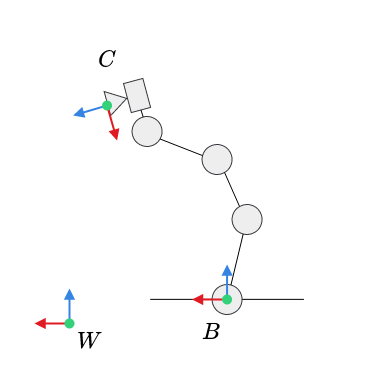
\includegraphics[width=\textwidth]{introduction/fig/eye_in_hand.png}
        \caption{Eye-in-hand setup.}
    \end{subfigure}
    % 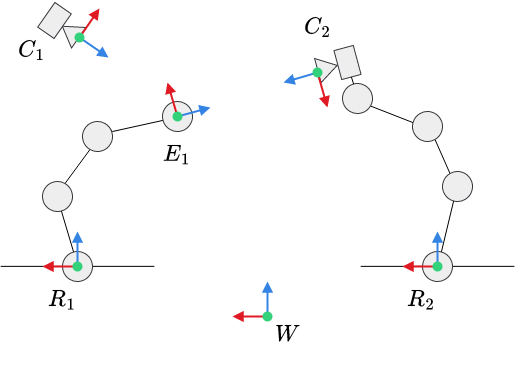
\includegraphics[width=\textwidth]{introduction/fig/eye_in_to_hand.png}
    \caption{Eye-to-hand, and eye-in-hand setups for serial arm manipulators. Camera frames $C$, robot base frame $B$, end-effector frame $E$ and world frame $W$. Real setups might consist of multiple robots. Refers to \secref{in:sec:spatial_awareness}.}
    \label{in:fig:coordinate_frames}
\end{figure}

\subsection{Camera Intrinsic Parameter Calibration}
\label{in:sec:camera_intrinsic_calibration}
Camera intrinsic parameters describe how 3D points are projected onto the observed 2D image plane. This image formation process is crucial for relating 3D points to 2D observations and vice-versa. Let $p_{_W}$ be a 3D point expressed in homogeneous coordinates with respect to the world frame $W$, $p_{_W} = \begin{bmatrix}
    x_{_W} & 1
\end{bmatrix}^T$, $x_{_W} = \begin{pmatrix}
    x_{_W} & y_{_W} & z_{_W}
\end{pmatrix}^T$. It is projected into the camera coordinate frame $C$ via a homogeneous transform $\homogeneous{C}{W}$ as

\begin{equation}
    p_{_C} = \homogeneous{C}{W} p_{_W}.
\end{equation}

Under the pinhole camera model, the point $p_{_C}$ is then projected onto the image plane via the intrinsic camera parameters $K$

% e.g. https://docs.opencv.org/4.x/dc/dbb/tutorial_py_calibration.html
% https://docs.opencv.org/4.x/d9/d0c/group__calib3d.html
\begin{equation}
    K = \begin{bmatrix}
        f_x & 0 & c_x \\
        0 & f_y & c_y \\
        0 & 0 & 1 \\
    \end{bmatrix},
\end{equation}

containing the focal lengths $f_{x/y}$, and the principal point $c_{x/y}$. Thus, the observed point in homogeneous image coordinates $u = \begin{pmatrix}
    u & v & 1
\end{pmatrix}^T$ is obtained through

\begin{equation}
    su = K P \homogeneous{C}{W} p_{_W},
\end{equation}

With $P = \begin{bmatrix}
    I^{3\times3} &  0
\end{bmatrix}$, simply being a projection matrix, and $s$ being a scalar usually set to $s = z_{_C}$ when $z_{_C} \neq 0$. Therefore yielding

\begin{equation}
    \begin{bmatrix}
        u \\
        v
    \end{bmatrix} = \begin{bmatrix}
        f_x x_c/z_c + c_x \\
        f_y y_c/z_c + c_y
    \end{bmatrix}.
\end{equation}

This projection assumes perfect optics, which is not the case in general. Real-world optics introduce radial and some tangential distortion. It is for this reason that distortion is accounted for via

\begin{equation}
    \begin{bmatrix}
        u \\
        v
    \end{bmatrix} = \begin{bmatrix}
        f_x x'' + c_x \\
        f_y y'' + c_y
    \end{bmatrix},
\end{equation}

with

\begin{equation}
    \begin{bmatrix}
        x'' \\
        y''
    \end{bmatrix}=\begin{bmatrix}
        x' \frac{1+k_1 r^2+k_2 r^4+k_3 r^6}{1+k_4 r^2+k_5 r^4+k_6 r^6}+2 p_1 x' y'+p_2\left(r^2+2 x^{\prime 2}\right)+s_1 r^2+s_2 r^4 \\
        y' \frac{1+k_1 r^2+k_2 r^4+k_3 r^6}{1+k_4 r^2+k_5 r^4+k_6 r^6}+p_1\left(r^2+2 y^{\prime 2}\right)+2 p_2 x' y'+s_3 r^2+s_4 r^4
    \end{bmatrix},
\end{equation}

\begin{equation}
    r^2 = x'^2 + y'^2,
\end{equation}

and

\begin{equation}
    \begin{bmatrix}
        x' \\
        y'
    \end{bmatrix} = \begin{bmatrix}
        x_c/z_c \\
        y_c/z_c
    \end{bmatrix}.
\end{equation}

Therein, $k_i$ are radial distortion coefficients, $p_i$ tangential distortion coefficients, and $s_i$ then prism coefficients. A camera calibration is performed through observing a pattern of known dimensions, e.g. a checkerboard, from various angles and positions, and optimizing for the model parameters, i.e. camera intrinsic parameters and distortion coefficients, such that the known projected points equal the observed and undistorted points.

\subsection{Eye-in-hand and Eye-to-hand Calibration}
\label{in:sec:eye_in_to_hand_calibration}
An overview of eye-in-hand and eye-to-hand setups is shown in \figref{in:fig:coordinate_frames}. Eye-in-hand calibration refers to the process of finding the camera frame $C$ to robot end-effector frame $E$ transformation $\homogeneous{E}{C}$ when the camera is attached to the robot's end-effector. Eye-to-hand calibration refers to finding the camera frame $C$ to robot base frame $B$ transformation $\homogeneous{B}{C}$ when the camera is statically placed next to the robot. A prerequisite for this type of calibration is a well known camera model, as was described in \secref{in:sec:camera_intrinsic_calibration}.

The calibration is performed by collecting target to camera $\homogeneous{T}{C}$ and robot base to end-effector transformations $\homogeneous{E}{B}$. Given undistorted camera images, and the camera intrinsic parameters, refer \secref{in:sec:camera_intrinsic_calibration}, target to camera transforms $\homogeneous{T}{C}$ can e.g. be obtained through solving a perspective-n-point (PnP) problem, where points are commonly obtained through ArUco markers, see \figref{in:fig:eye_in_hand_setup}. The base to end-effector transformation $\homogeneous{E}{B}$ can be obtained through robot kinematics.
\begin{figure}
    \centering
    \begin{subfigure}[b]{0.49\textwidth}
        \centering
        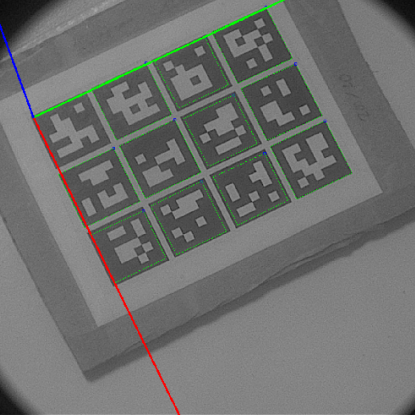
\includegraphics[width=\textwidth]{introduction/img/aruco.png}
        \caption{Undistorted exoscope view of the ArUco marker target.}
    \end{subfigure}
    \begin{subfigure}[b]{0.49\textwidth}
        \centering
        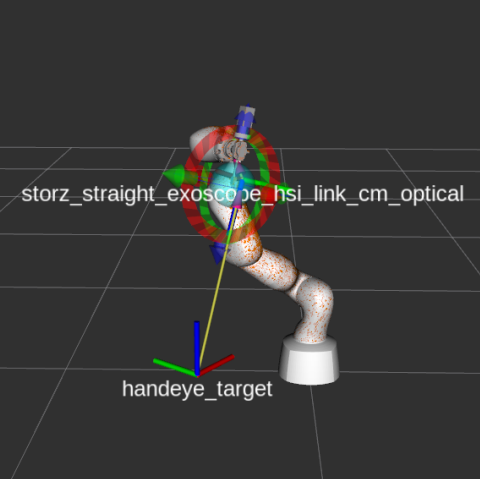
\includegraphics[width=\textwidth]{introduction/img/aruco_world.png}
        \caption{Mesh visualization of robot state with estimated camera and target poses.}
    \end{subfigure}
    \caption{Eye-in-hand calibration example in a realistic scenario. Used hardware includes: Storz VITOM Telescope $0^\circ$ w Integ. Illuminator., Storz TH 102 H3-Z FI camera head, and KUKA LBR Med7 R800. Refers to \secref{in:sec:eye_in_to_hand_calibration}.}
    \label{in:fig:eye_in_hand_setup}
\end{figure}
In both, the eye-in-hand and eye-to-hand scenario, it is known that the transformation from end-effector to camera $\homogeneous{C}{E}$ and end-effector to target $\homogeneous{E}{T}$, respectively, remains unchanged. Therefore, recording transforms, e.g. for the eye-in-hand setup, in two configurations lets one determine

\begin{equation}
    \homogeneous{B}{E}^{1}\homogeneous{E}{C}\homogeneous{C}{T}^{1} = \homogeneous{B}{E}^{2}\homogeneous{E}{C}\homogeneous{C}{T}^{2},
\end{equation}

which can be re-arranged as

\begin{equation}
    \homogeneous{E}{B}^{2}\homogeneous{B}{E}^{1}\homogeneous{E}{C} = \homogeneous{E}{C}\homogeneous{C}{T}^{2}\homogeneous{T}{C}^{1},
\end{equation}

thus yielding an equation of the form $AX = XB$ with $A=\homogeneous{E}{B}^{2}\homogeneous{B}{E}^{1}$ and $B=\homogeneous{C}{T}^{2}\homogeneous{T}{C}^{1}$. Solving for $X=\homogeneous{E}{C}$ provides the desired eye-in-hand transformation. Similarly, a system of the form $AX = XB$ can be derived for the eye-to-hand setup. A system of this form can e.g. be solved using \cite{tsai1989new, park1994robot, horaud1995hand}.

% good video: https://www.youtube.com/watch?v=xQ79ysnrzUk
% https://docs.opencv.org/4.5.4/d9/d0c/group__calib3d.html#gaebfc1c9f7434196a374c382abf43439b

\subsection{Unified Calibration for Optimal Clinical Workflow}
\label{in:sec:unified_calibration}
Having a solid understanding of the calibrations that are required for this thesis, we will now investigate the question of applicability within the clinical context. When applied within the clinical scenario, e.g. for collision avoidance or autonomous control, as was explained in \secref{in:sec:enhancing_current_systems}, it is of utmost importance that the clinical workflow must not be disturbed. In this section, implications of the different calibrations to the clinical workflow will be discussed. Following that, the idea of marker-free calibration is introduced, and it is explained how the introduced clinical workflow constraints could be resolved.

\subsubsection{Implications of Calibrations to the Clinical Workflow}
As discussed in the above, \secref{in:sec:camera_intrinsic_calibration} and \secref{in:sec:eye_in_to_hand_calibration}, calibrations require calibration targets. In current practise, the necessity of a calibration target would add overhead to the clinical workflow. Calibrations also depend on the type of camera used, which refers back to \secref{in:sec:automation} - Robot-free Surgeries. Standard laparoscopic camera heads are detachable for sterilization of the laparoscope and provide an adjustable focus. Both of which potentially alter the camera intrinsic parameters and would make re-calibration necessary. For the remainder of this thesis, we will therefore assume that the focal length stays fixed in a range appropriate for surgery. Furthermore, we will assume that the camera head does not rotate about the optics. This assumption is, however, not as crucial for the camera intrinsic calibration, since surgery optics are of extremely high quality with very little distortion. It is more relevant for eye-in-hand calibrations, where the obtained camera pose is crucial for control. For any external camera, these assumptions do not need to be made and they are allowed to move freely.

The implications of calibrations to the clinical workflow refer back to \figref{in:fig:advancing_robotic_laparoscopy}, where additional operation time and surgeon convenience were identified as vital aspects for the shortcomings and advantages of RMIS, respectively. An overview of the implications of the different calibrations is provided in \tabref{in:tab:calibrations}.
\begin{table}[]
\centering
\caption{The implications of different calibrations to the clinical workflow. Refers to camera intrinsics calibration (\secref{in:sec:camera_intrinsic_calibration}), eye-in/to-hand calibration (\secref{in:sec:eye_in_to_hand_calibration}), and \secref{in:sec:unified_calibration}.}
\label{in:tab:calibrations}
\begin{tabular}{@{}lll@{}}
\toprule
Calibration Type  & Offline       & Clinical Workflow Implications \\ \midrule
Camera intrinsics & Cond.         & Camera head ideally static with fixed focus \\
Eye-in-hand       & Cond. & Camera pose fixed and known, else re-calibrated \\
Eye-to-hand       & No            &  Calibration online. Devices may not be moved \\ \bottomrule
\end{tabular}
\end{table}
As can be seen, only the camera intrinsic parameter calibration, in principle, has very little impact on clinical workflow. This, again, is not always the case in classical laparoscopy, especially for the commonly used detachable camera heads, e.g. \figref{in:fig:eye_in_hand_setup}, which, depending on the mounting orientation and adjustable focal length, influence camera intrinsic parameters and eye-in-hand calibration parameters. For automation purposes, it should therefore be enforced that these parameters are known and remain unchanged. For spatial awareness, the constraints are less restricting, since an external camera suffices to estimate robot poses. The external camera's intrinsic parameters can fully be determined offline, therefore keeping the clinical workflow untouched. In this case, however, it is still necessary to use a calibration target, which introduces inconvenience and mental burden to the surgeon and clinical staff. We argue that it is for this reason that surgical robots are currently spatially unaware, which causes additional operating time and inconvenience, as was explained in \secref{in:sec:spatial_awareness}. We will therefore introduce the idea of marker-free calibration for eye-to-hand setups, but also eye-in-hand setups to alleviate some of the shortcomings in the following section.

\subsubsection{Marker-free Unified Calibration}
Having the clinical workflow implications like the necessity for calibration targets in mind, it becomes apparent that alternative solutions for calibrations might be desirable. Recent works have, therefore, focused on utilizing the robot itself as calibration target. The idea is simple, the robot mesh, given the current robot configuration, see e.g. \figref{in:fig:eye_in_hand_setup}, is compared against the real robot, thus allowing to estimate camera position with respect to the robot. Initial work estimates joint positions from images and solves a PnP problem, given the robot kinematics to estimate poses \cite{labbe2021single}. Other work performs differentiable rendering for increased accuracy \cite{chen2023easy}, and some turn PnP and differentiable rendering into a self-supervised problem \cite{lu2023markerless}.

Since we are mostly interested in estimating the robot pose in eye-to-hand scenarios, as was described in \secref{in:sec:enhancing_current_systems}, and due to the difficulties with eye-in-hand setups with laparoscopic cameras, as was explained in the above section, this work will mostly focus on using external cameras for pose estimation rather than the laparoscope itself. We will be assuming access to a stereo camera, therefore deviating from the above works and simplifying the registration task greatly. This should improve registration reliability, which is important for surgery. The following sections will explain an iterative closest point registration on Lie-algebra for said purpose in \secref{in:sec:p2plane}. Following that, image-based registration refinements, given a segmentation mask without the need for differentiable rendering are explained in \secref{in:sec:registration_of_3d_point_cloud}.

% Tom's notes
% \subsubsection{Point-to-plane ICP: A Lie Algebra Formulation}
% \label{in:sec:p2plane}

\paragraph{Basic Formulation}
We first introduce the problem solved by the point-to-plane \gls{icp} algorithm~\cite{Rusinkiewicz:IC3DIM:2001}.
Let $\mathbf{p}_i$ and $\mathbf{q}_i$ be corresponding 3D points in homogeneous coordinates. Let $\mathbf{n}_i$ be a normal vector associated with $\mathbf{q}_i$. We search a rigid body transformation $\mathbf{\Theta}$ in $SE(3)$ that minimizes:
\begin{equation}
\sum_i ||\mathbf{n}_i^T \cdot (\mathbf{\Theta} \cdot \mathbf{p}_i - \mathbf{q}_i)||^2 = \sum_i (\mathbf{n}_i^T \cdot \mathbf{\Theta} \cdot \mathbf{p}_i - \mathbf{n}_i^T \cdot \mathbf{q}_i)^2
\end{equation}

\paragraph{Iterative Optimization on the $SE(3)$ Lie Group}
Let $\mathbf{\Theta}_0$ be the current estimate. In a Lie group iterative optimization approach~\cite{Mahony:JGO:2002,Vercauteren:IPMI:2007}, we seek a perturbation $\Delta\mathbf{\Theta} \in \mathfrak{se}(3)$ composed with
$\mathbf{\Theta}_0$: $\mathbf{\Theta}_1 = \mathbf{\Theta}_0 \cdot \exp(\Delta\mathbf{\Theta})$. We now seek to minimize:
\begin{equation}
\sum_i (\mathbf{n}_i^T \cdot \mathbf{\Theta}_0 \cdot \exp(\Delta\mathbf{\Theta}) \cdot \mathbf{p}_i - \mathbf{n}_i^T \cdot \mathbf{q}_i)^2
\end{equation}

\paragraph{Mathematical Preliminaries}
For convenience, we take advantage of the relationship between the 3D cross product, the Lie bracket on SO(3), and the skew-symmetric matrix operator.
Let $\boldsymbol{\omega} = [\omega_x, \omega_y, \omega_z]^T$ and $\boldsymbol{\eta} = [\eta_x, \eta_y, \eta_z]^T$ be two 3D vectors, we have
\begin{equation}
[\boldsymbol{\omega}, \boldsymbol{\eta}] = \boldsymbol{\omega} \times \boldsymbol{\eta} = \boldsymbol{\omega}_\times \boldsymbol{\eta}
\end{equation}
where
\begin{equation}
\boldsymbol{\omega}_\times =
\begin{bmatrix}
0         & -\omega_z & \omega_y \\
\omega_z  & 0         & -\omega_x \\
-\omega_y & \omega_x  & 0
\end{bmatrix}
\end{equation}

It can be shown that the Lie group exponential in SO(3) admits a closed form through the Rodrigues’ formula. Let us consider $\boldsymbol{\omega}$ as an element of $\mathfrak{so}(3)$, we now have
\begin{equation}
\expl(\boldsymbol{\omega}) = \exp(\boldsymbol{\omega}_\times) = \mathbf{I}^{3\times3} + \frac{\sin(||\boldsymbol{\omega}||)}{||\boldsymbol{\omega}||}\boldsymbol{\omega}_\times + \frac{1-\cos(||\boldsymbol{\omega}||)}{||\boldsymbol{\omega}||^2}\boldsymbol{\omega}_\times^2
\end{equation}
which for small values of $||\boldsymbol{\omega}||$ leads to the following numerically stable approximation
\begin{equation}
\expl(\boldsymbol{\omega}) \approx \mathbf{I}^{3\times3}
+ (1-\frac{||\boldsymbol{\omega}||^2}{6}+\frac{||\boldsymbol{\omega}||^4}{120})\boldsymbol{\omega}_\times
+ (\frac{1}{2}-\frac{||\boldsymbol{\omega}||^2}{24}+\frac{||\boldsymbol{\omega}||^4}{720}))\boldsymbol{\omega}_\times^2
\end{equation}

\iffalse
For compatibility with the 3D cross product, we choose the following basis for the matrix representation of $\mathfrak{se}(3)$:
\begin{align}
e_1 &= 
\begin{bmatrix}
0 & 0 & 0  & 0 \\
0 & 0 & -1 & 0 \\
0 & 1 & 0  & 0 \\
0 & 0 & 0  & 0
\end{bmatrix}
\\
e_2 &=
\begin{bmatrix}
0  & 0 & 1 & 0 \\
0  & 0 & 0 & 0 \\
-1 & 0 & 0 & 0 \\
0  & 0 & 0 & 0
\end{bmatrix}
\\
e_3 &=
\begin{bmatrix}
0 & -1 & 0 & 0 \\
1 & 0  & 0 & 0 \\
0 & 0  & 0 & 0 \\
0 & 0  & 0 & 0
\end{bmatrix}
\\
e_4 &=
\begin{bmatrix}
0 & 0 & 0 & 1 \\
0 & 0 & 0 & 0 \\
0 & 0 & 0 & 0 \\
0 & 0 & 0 & 0
\end{bmatrix}
\\
e_5 &=
\begin{bmatrix}
0 & 0 & 0 & 0 \\
0 & 0 & 0 & 1 \\
0 & 0 & 0 & 0 \\
0 & 0 & 0 & 0
\end{bmatrix}
\\
e_6 &=
\begin{bmatrix}
0 & 0 & 0 & 0 \\
0 & 0 & 0 & 0 \\
0 & 0 & 0 & 1 \\
0 & 0 & 0 & 0
\end{bmatrix}
\end{align}
\fi

Let us consider a 6D vector $\mathbf{u}=[\boldsymbol{\omega};\boldsymbol{\tau}]$ as an element of $\mathfrak{se}(3)$. Its matrix representation is provided by
\begin{equation}
  \mathbf{u}_\dagger =
\begin{bmatrix}
\boldsymbol{\omega}_\times & \boldsymbol{\tau} \\
0  & 0
\end{bmatrix} \in \mathbb{R}^{4\times4}
\end{equation}
which leads to the following closed-form formula for the Lie group exponential for SE(3):
\begin{equation}
\expl(\mathbf{u}) = \exp(\mathbf{u}_\dagger) =
\begin{bmatrix}
\expl(\boldsymbol{\omega}) & L(\boldsymbol{\omega})\boldsymbol{\tau} \\
0  & 1
\end{bmatrix}
\end{equation}
where
\begin{equation}
L(\boldsymbol{\omega}) = \mathbf{I}^{3\times3}
+ \frac{1-\cos(||\boldsymbol{\omega}||)}{||\boldsymbol{\omega}||^2}\boldsymbol{\omega}_\times
+ \frac{||\boldsymbol{\omega}||-\sin(||\boldsymbol{\omega}||)}{||\boldsymbol{\omega}||^3}\boldsymbol{\omega}_\times^2
\end{equation}
where a Taylor expansion should again be used for numerical stability if $||\boldsymbol{\omega}||$ is small:
\begin{equation}
L(\boldsymbol{\omega}) \approx \mathbf{I}^{3\times3}
+ (\frac{1}{2}-\frac{||\boldsymbol{\omega}||^2}{24}+\frac{||\boldsymbol{\omega}||^4}{720})\boldsymbol{\omega}_\times
+ (\frac{1}{6}-\frac{||\boldsymbol{\omega}||^2}{120}+\frac{||\boldsymbol{\omega}||^4}{5040})\boldsymbol{\omega}_\times^2
\end{equation}

\paragraph{First-order Linearization of the Action of the Exponential in $\mathfrak{se}(3)$}
Let $\mathbf{p}=[\tilde{\mathbf{p}};1]$ be a 3D point in homogeneous coordinates. We consider an infinitesimal element $\Delta \mathbf{u}=[\Delta \boldsymbol{\omega};\Delta \boldsymbol{\tau}]$ of $\mathfrak{se}(3)$ and consider the corresponding action on $p$:
\begin{equation}\label{eq:lieactionlinearisation}
\begin{split}
\expl(\Delta \mathbf{u})\mathbf{p} &\approx (\mathbf{I}^{4\times4}+\Delta \mathbf{u}_\dagger)\mathbf{p} = \mathbf{p} +
\begin{bmatrix}
\Delta \boldsymbol{\omega}_\times & \Delta \boldsymbol{\tau} \\
0  & 0
\end{bmatrix} \mathbf{p}
= \mathbf{p} +
\begin{bmatrix}
\Delta \boldsymbol{\omega}_\times \tilde{\mathbf{p}}+\Delta \boldsymbol{\tau} \\
0
\end{bmatrix} \\
&= \mathbf{p} +
\begin{bmatrix}
\Delta \boldsymbol{\omega} \times \tilde{\mathbf{p}}+\Delta \boldsymbol{\tau} \\
0
\end{bmatrix}
= \mathbf{p} +
\begin{bmatrix}
-\tilde{\mathbf{p}} \times \Delta \boldsymbol{\omega} + \Delta \boldsymbol{\tau} \\
0
\end{bmatrix} \\
&= \mathbf{p} +
\begin{bmatrix}
-\tilde{\mathbf{p}}_\times & \mathbf{I}^{3\times3} \\
0 & 0
\end{bmatrix} \Delta \mathbf{u}
= \mathbf{p} + \mathbf{D}(\mathbf{p})\Delta \mathbf{u}
\end{split}
\end{equation}
where
\begin{equation}
\mathbf{D}(\mathbf{p}) = 
\begin{bmatrix}
-\tilde{\mathbf{p}}_\times & \mathbf{I}^{3\times3} \\
0 & 0
\end{bmatrix} \in \mathbb{R}^{4\times6}
\end{equation}

\paragraph{Lie Algebra Linearization of the Point-to-plane Objective}
Plugging \eqref{eq:lieactionlinearisation} in the original point-to-plane ICP cost function we get the following linearization:
\begin{equation}
\begin{split}
\sum_i & \Big(\mathbf{n}_i^T \mathbf{\Theta}_0 \big(\mathbf{p}_i + \mathbf{D}(\mathbf{p}_i)\Delta\mathbf{\Theta} \big) - \mathbf{n}_i^T \mathbf{q}_i\Big)^2
\\
&= \sum_i \Big(\mathbf{n}_i^T \mathbf{\Theta}_0 \mathbf{D}(\mathbf{p}_i)\Delta\mathbf{\Theta} + \mathbf{n}_i^T \mathbf{\Theta}_0 \mathbf{p}_i - \mathbf{n}_i^T \mathbf{q}_i\Big)^2
\end{split}
\end{equation}
Denoting $\mathbf{a}_i = \mathbf{n}_i^T \mathbf{\Theta}_0 \mathbf{D}(\mathbf{p}_i)$, $\mathbf{A}=[\mathbf{a}_0;\ldots;\mathbf{a}_N]$,
$b_i = \mathbf{n}_i^T (\mathbf{q}_i - \mathbf{\Theta}_0 \mathbf{p}_i)$, and $\mathbf{B}=[b_0;\ldots;b_N]$, we end up with a standard linear least squares problem:
\begin{equation}\label{eq:icplls}
||\mathbf{A} \Delta\mathbf{\Theta} - \mathbf{B}||^2
\end{equation}
which can conveniently be expressed using the pseudo-inverse $\mathbf{A}^{\dagger}$ of $\mathbf{A}$:
\begin{equation}
\Delta\mathbf{\Theta} = \mathbf{A}^{\dagger} \mathbf{B}
\end{equation}

In practice, given the dimensions of $\mathbf{A}$, $b$ and $\Delta\mathbf{\Theta}$, \eqref{eq:icplls} is probably best solved by using the normal equations
\begin{equation}
(\mathbf{A}^T \mathbf{A}) \Delta\mathbf{\Theta} = \mathbf{A}^T \mathbf{B}
\end{equation}
and relying on a Cholesky decomposition:
\begin{equation}
\Delta\mathbf{\Theta} = \texttt{chol\_solve}(\mathbf{A}^T \mathbf{A}, \mathbf{A}^T \mathbf{B})
\end{equation}

Note that by expressing $\mathbf{A}$ and $\mathbf{B}$ without homogeneous coordinates, we get:
\begin{equation}
\mathbf{a}_i = [-\tilde{\mathbf{n}}_i^T \mathbf{R}_0 {{\tilde{\mathbf{p}}}_{i\times}}, \tilde{\mathbf{n}}_i^T \mathbf{R}_0] \in \mathbb{R}^{1\times6}
\end{equation}
and
\begin{equation}
b_i = \tilde{\mathbf{n}}_i^T (\tilde{\mathbf{q}}_i - \mathbf{R}_0 \tilde{\mathbf{p}}_i - T_0) \in \mathbb{R}
\end{equation}

\paragraph{Robust Formulation}
To reduce the influence of outliers on the solution, a typical approach is to introduce a
loss function $\rho_\kappa$ parameterized by a scale parameter (a.k.a. soft margin or cut-off) $\kappa$ to scale the residuals. We then seek to minimize:
\iffalse
\begin{equation}
\sum_i \rho\big(\frac{1}{C^2}(\mathbf{n}_i^T \cdot \mathbf{\Theta} \cdot \mathbf{p}_i - \mathbf{n}_i^T \cdot \mathbf{q}_i)^2\big)
\end{equation}

Using the identity loss function $\rho(z)=z$ leads to the original least-squares problem. Classical robust alternatives include:
\begin{description}
  \item[Soft L1]:
  $\rho(z) = 2 (\sqrt{1 + z} - 1)$.
  The smooth approximation of l1 (absolute value) loss. Usually a good choice for robust least squares.

  \item[Huber]:
  $\rho(z) = z \texttt{ if } z <= 1 \texttt{ else } 2\sqrt{z} - 1$.
  Works similarly to ``Soft L1".

  \item[Cauchy]:
  $\rho(z) = \ln(1 + z)$.
  Severely weakens outliers influence, but may cause difficulties in optimization process.

   \item[Arctan]:
   $\rho(z) = \arctan(z)$.
   Limits a maximum loss on a single residual, has properties similar to ``Cauchy".
\end{description}
\fi
\begin{equation}
\sum_i \rho_k\Big(\mathbf{n}_i^T \cdot \mathbf{\Theta} \cdot \mathbf{p}_i - \mathbf{n}_i^T \cdot \mathbf{q}_i\Big)
\end{equation}
or equivalently if we start from a given estimate in the above Lie group setting:
\begin{equation}
\sum_i \rho_k\Big(\mathbf{a}_i \Delta\mathbf{\Theta} - b_i\Big)
\end{equation}
%
Using the square loss function $\rho_\kappa(z)=z^2$ leads to the original least-squares problem. A classical robust alternatives is the Huber loss
\begin{equation}
\rho_\kappa(z) =
\begin{cases}
  z^2 &\texttt{ if } |z| <= \kappa \\
  2|z|\kappa - \kappa^2  &\texttt{ otherwise }
\end{cases}
\end{equation}
with $\kappa=1.345\sigma$ being advocated to provide robustness while retaining appropriate properties when the errors are Gaussian.

This minimisation can be achieved by a standard \gls{irls} approach~\cite{Green:JRSSB:1984} or by including a second order terms in a slightly more advanced reweighted Gauss-Newton approach as discussed in~\cite{Triggs:VisAlg:2000}.
The latter is referred to as the Triggs correction in \footnote{\url{http://ceres-solver.org/nnls_modeling.html\#theory}}. While elegant, previous work has shown that the Triggs correction does not significantly improve on the standard \gls{irls}~\cite{Zach:ECCV:2014,Zach:ECCV:2018}.
Here, for simplicity we thus restrict ourselves to standard \gls{irls}.
Given a choice of scaling factor $\kappa$ and an estimate of the parameters $\mathbf{\Theta}$, the robust problem is converted to a weighted least-squares:
\begin{equation}
\sum_i \omega_\kappa(b_i) ||\mathbf{a}_i \Delta\mathbf{\Theta} - b_i||^2
\end{equation}
with $\omega_\kappa(z) = \rho'_\kappa(z) / z$ being the weight function associated with the Huber loss:
\begin{equation}
\omega_\kappa(z) =
\begin{cases}
  1 &\texttt{ if } |z| <= \kappa \\
  \kappa / |z|  &\texttt{ otherwise }
\end{cases}
\end{equation}

This leads us to the following weighted normal equation:
\begin{equation}
(\mathbf{A}^T \mathbf{W} \mathbf{A}) \Delta\mathbf{\Theta} = \mathbf{A}^T \mathbf{W} \mathbf{B}
\end{equation}
where $\mathbf{W} = \diag\big(\omega_\kappa(b_0), \ldots, \omega_\kappa(b_N)\big)$.

One aspect we haven't addressed yet it the choice of $\kappa$ for the Huber loss. As mentioned earlier, a typical choice is to use $\kappa=1.345\sigma$. We are thus left with the need to robustly estimate the standard deviation of the residuals. This is typically done through a \gls{mad}:
\begin{equation}
\hat{\sigma} = \frac{\MAD(\{b_i\})}{0.6745} = \frac{\median(\{|b_i-\median(\{b_i\}|)\})}{0.6745}
\end{equation}

%% unused section in PhD thesis
% \subsubsection{Registration of a 3D Point Cloud with 2D Stereo Segmentations}
% \label{in:sec:registration_of_3d_point_cloud}
% %
% Let $\mathbf{q}_i$ be 3D points associated to a model object as expressed in an object specific coordinate frame.
% Let $I_L$ and $I_R$ be a pair of stereo images with associated $M_L$ and $M_R$ camera matrices (including both extrinsic and intrinsic).
% We assume that the stereo images are observing the object in an unknown pose $\mathbf{\Theta}$.
% We also assume that the object is relatively textureless and that we do not have a good means of extracting keypoints of interest from the images.
% We however assume that a segmentation of the object in each image can readily be computed, e.g. with the \gls{sam}~\cite{Kirillov:iccv:2023}.
% %
% While differentiable rendering could be used in this context~\cite{Hannemose:SPIE:2019,labbe2021single,Chen:RAL:2023},
% we expect that a simpler algorithm can be designed given the segmentation availability by matching points from 3D to 2D.
% We also expect to potentially gain robustness against illumination and other factors that would impact the appearance of the object in the images.

% Let $S_L$ and $S_R$ be the object segmentation masks in the left and right image respectively.
% We here seek to recover the pose $\mathbf{\Theta}$ such that the projected model points ${M_L \mathbf{\Theta} q}$ match the observed segmentation $S_L$ (respectively ${M_R \mathbf{\Theta} q}$ to match $S_R$).
% Let $\varphi$ be a function to transform from homogeneous to Cartesian coordinates.
% That is $\varphi([x,y,f])=[x/f,y/f]$ and similarly in 3D.
% We can write the objective as:
% \begin{equation}
% \arg\min_{\mathbf{\Theta}} \sum_i
% \min_{p_L|S_L(p_L)=1}|| \varphi\big(M_L \mathbf{\Theta} \mathbf{q}_i\big) - p_L||^2
% + \min_{p_R|S_R(p_R)=1}|| \varphi\big(M_R \mathbf{\Theta} \mathbf{q}_i\big) - p_R||^2
% \end{equation}

% Similar to the approach in~\cite{Fitzgibbon:IVC:2003}, this formulation can be substantially accelerated by taking advantage of the fact that the segmentations are defined on a regular grid. We can thus use a \gls{edt} for which optimized algorithms exist on both \gls{cpu}~\cite{Felzenszwalb:TC:2012}\footnote{\url{https://github.com/cai4cai/distance_transform}} and \gls{gpu}~\cite{Cao:SIGGRAPH:2010}\footnote{\url{https://docs.rapids.ai/api/cucim/stable/api/\#cucim.core.operations.morphology.distance_transform_edt}}.
% Let $\mathcal{D}_{S_L}$ be the \gls{edt} computed from $S_L$ (respectively $\mathcal{D}_{S_R}$ for $S_R$).
% We can now write
% \begin{equation}\label{eq:dt3d2d}
% \arg\min_{\mathbf{\Theta}} \sum_i \mathcal{D}_{S_L}^2\big( \varphi(M_L \mathbf{\Theta} \mathbf{q}_i) \big)
% + \mathcal{D}_{S_R}^2\big( \varphi(M_R \mathbf{\Theta} \mathbf{q}_i) \big)
% \end{equation}

% As in \secref{in:sec:p2plane}, the square loss terms could be replaced by robust alternatives.
% It should further be noted that the evaluation of a distance transform $\mathcal{D}_{S}$ at an arbitrary point $p$ requires the use of an interpolator.
% A typical choice is to rely on bilinear interpolation for which optimized implementations exist on both \gls{cpu} and \gls{gpu}\footnote{\url{https://pytorch.org/docs/stable/generated/torch.nn.functional.grid_sample.html}}.

% Solving for \eqref{eq:dt3d2d} can be done again by taking advantage of the Lie group structure of SE(3). For simplicity, a generic Lie group non-linear least-squares optimizer as found in Theseus\footnote{\url{https://github.com/facebookresearch/theseus}}~\cite{Pineda:NeurIPS:2023} or Ceres\footnote{\url{https://github.com/ceres-solver/ceres-solver}}~\cite{Agarwal:Ceres:2022} can be used.

% It is worth realising that even if a rigid body model is used, formulation \eqref{eq:dt3d2d} may have somewhat trivial solutions if configurations can be found where the projected 2D point set can fit completely inside of the object segmentation mask as this would lead to a zero loss. It may thus be advantageous to somewhat also consider points outside of the model and make sure that these stay outside of the segmentation mask.


\section{Camera Motion Automation in Robotic Laparoscopy}
\label{in:sec:camera_motion_automation}
Having established a proper understanding of the importance of spatial awareness for RMIS in general (\secref{in:sec:spatial_awareness}), and for automation in particular, this section will investigate camera motion automation in robotic laparoscopy, which was identified as the second desired enhancement in RMIS, \secref{in:sec:enhancing_current_systems}, \figref{in:fig:advancing_robotic_laparoscopy}. Initially, several alternatives for laparoscopic camera motion automation will be discussed in \secref{in:sec:automation_approaches}. Of these methods, and due its promising properties, visual servoing will be investigated further. Starting with rule-based approaches to visual servoing and relevant auxiliary tasks like tool segmentation in \secref{in:sec:rule_based_approaches}, the reader will be introduced to limitations of such methods, that is assumptions to laparoscopy that generally do not hold in real surgery. To find a potential solution, the focus is shifted towards data-driven methods. The data-driven methods include reinforcement learning (RL) and imitation learning (IL). Since data-driven methods are relatively new to laparoscopic camera motion automation, a broad review to RL will be given in \secref{in:sec:reinforcement_learning}, followed by IL in \secref{in:sec:imitation_learning}.

\subsection{Camera Motion Automation Approaches}
\label{in:sec:automation_approaches}
\begin{figure}
    \centering
    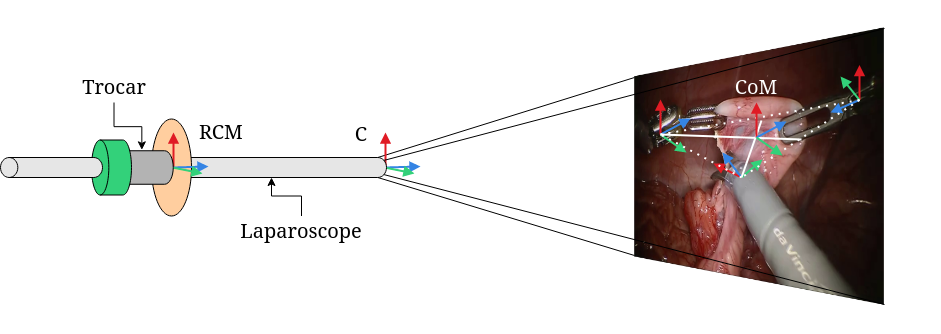
\includegraphics[width=\textwidth]{introduction/fig/rule_based_approaches.png}
    \caption{Coordinate frames relevant for laparoscopic camera motion automation. Camera frame C, center of mass frame CoM, and RCM at trocar. The camera frame C is commonly obtained via eye-in-hand calibration, \secref{in:sec:eye_in_to_hand_calibration} and \figref{in:fig:eye_in_hand_setup}. For visual servoing, the CoM assumption as view center-point in commonly made. Laparoscopic view shows an image from a da Vinci\textsuperscript{\textregistered} system in the SurgVisDom\cite{zia2021surgical} dataset. Refers to \secref{in:sec:rule_based_approaches}.}
    \label{in:fig:com}
\end{figure}
Laparoscopic camera motion can be automated in a plenitude of ways. A typical laparoscopic setup is shown in \figref{in:fig:com}. Therein, the ultimate goal is to control the pose of the camera frame C under the RCM constraint. The camera frame C, as was explained in 
\secref{in:sec:camera_intrinsic_calibration}, and \secref{in:sec:eye_in_to_hand_calibration}, \figref{in:fig:eye_in_hand_setup}, can be obtained through camera intrinsic parameters plus eye-in-hand calibration.

In fully robotic setups, a common approach to automation is to simply use the kinematic data that is available through the joint position encoders \cite{da2020scan}. The camera then follows some geometric point, like the center of mass between the tools, as shown in \figref{in:fig:com}. Without the kinematic data, these methods are not be applicable to hybrid setups, which are of particular interest to this work, as was mentioned in \secref{in:sec:automation} - Robot-free surgeries. They further suffer some other shortfalls, such as the inability to obey by anatomic constraints and reliance on accurate multi-arm calibrations. Other, semi-autonomous techniques, aim to alleviate some of the model uncertainties by assigning the surgeons a greater responsibility to controlling the camera in a collaborative fashion. Gaze or voice control are among them \cite{taniguchi2010classification}. They, however, lead to eye strain, additional mental workload or communication failures, and do not satisfy the - level five: high autonomy - target that was set in \secref{in:sec:foreword}.

Alongside automation via kinematic data, visual servoing, i.e. control through images, is considered a promising alternative, as it provides intra-operative feedback \cite{pandya2014review} and is less prone to errors from model mismatch \cite{azizian2014visual}. It is capable of understanding and interpreting the surgical scene, thus potentially enabling level five autonomy and above, the overarching goal of this work, \secref{in:sec:foreword}. Visual servoing, in itself, is of special interest to this work for one additional reason.
\begin{figure}
    \centering
    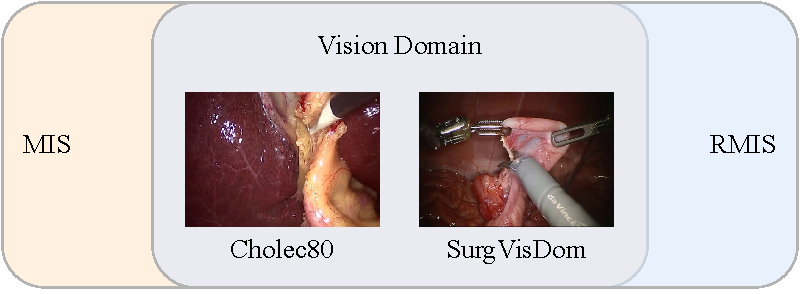
\includegraphics{introduction/fig/shared_domain.pdf}
    \caption{The vision domain is a shared domain between MIS and RMIS procedures. Laparoscopic views taken from Cholec80 \cite{twinanda2016endonet}, and SurgVisDom. \cite{zia2021surgical}. Refers to \secref{in:sec:automation_approaches}.}
    \label{in:fig:shared_domain}
\end{figure}
It characterizes MIS to RMIS transferability, as was targeted in \secref{in:sec:enhancing_current_systems}. Vision poses a shared domain between MIS and RMIS, the vision domain, as shown in \figref{in:fig:shared_domain}. Visual servoing methodologies could thus be transferred from MIS to RMIS and vice-versa. In the next section, we will, therefore, review rule-based visual servoing approaches.

\subsection{Rule-based Visual Servoing}
\label{in:sec:rule_based_approaches}
Rule-based visual servoing approaches are a well established research field for laparoscopic camera motion automation. These methods are formulating control through specifying some proxy for autonomy. There exists research on visual servoing with mechanical RCM and visual servoing with programmable RCM. Although areas aim at controlling the camera frame, refer \figref{in:fig:com}, we will distinguish between them for better clarity and to comply with the targets that were outlined in \secref{in:sec:enhancing_current_systems}. The following two paragraphs will, therefore, review current rule-based approaches with mechanical and programmable RCM, respectively, followed by a paragraph that analyzes the shortcomings of these methods.

\paragraph{Visual Servoing with mechanical RCM}
Approaches that use a mechanical RCM are \cite{omote1999self}, where a visual servo is implemented to control the center of mass of a colored marker on a forceps in image space. In \cite{agustinos2014visual, voros2007automatic}, the tool tip position is found in image space via kinematic knowledge over the tool entry points and a visual servo is applied to center the tool tip in image space. Another common scheme is to alter the camera's zoom based on the distance of the surgical tools, which was first presented in \cite{king2013towards}, where the authors use colored markers to track the surgical instruments.

The authors in \cite{eslamian2020development, mariani2020experimental, da2020scan}, with related prior works in \cite{Eslamian2016TowardsTI, eslamian2017autonomous}, compute the center point in between two surgical tools via their respective positions and align the camera's optical axis with the line that spans from RCM to the tools' center point, which requires a complicated registration procedure. \cite{yu2016automatic} also relies on the positions of the surgical tools and adjusts the field of view's width based on the distance of them. \cite{abdelaal2020orientation} uses a similar approach as \cite{eslamian2020development}, in that they adjust the camera distance to the surgical scene based on the tool distance, however, they don't align the camera's optical axis with the line that spans from RCM to the camera, but rather with the scene's surface normal, which is made possible by their 6 DoF endoscope. In \cite{ma2019autonomous}, Ma et al. deploy a visual servo to center a green marker on a tool by incorporating depth information as extracted from camera and tool motion. In \cite{ma2020visual} they extend this work into a quadratic program in which they minimize joint velocities whilst constraining the camera's distance with respect to the tools and the average tool position in the image plane to be central, where they rely on stereoscopic images to extract depth information. \cite{gruijthuijsen2021autonomous} propose a framework for semantically rich collaborative control but effectively only track surgical tools.

\paragraph{Visual Servoing with programmable RCM}
Where a mechanical RCM is not available, it can be achieved programmatically. As such, \cite{aghakhani2013task} design a composite Jacobian method that integrates a RCM objective with a task function that defines an error on points in image space. The authors in \cite{yang2019adaptive} also design a Jacobian gain controller that enforces the tip of a tool to reside within a defined region by computing the winding number of that region around the desired point. They additionally request the endoscope to extend the surgeon's natural line of sight. In \cite{li2020accelerated}, Li et al. introduce the RCM and a visual error via the image Jacobian as constraints to a quadratic problem that aims at satisfying these constraints whilst minimizing the joint velocities. \cite{sandoval2021towards} propose a torque control framework that includes remote center of motion constraints, tool center point following and nullspace projects for arm-staff collisions.

\paragraph{Flaws of current Visual Servos} It becomes apparent that most of these methods rely on the mere tool distance to infer a control law, whereas only in \cite{ma2019autonomous, ma2020visual, aghakhani2013task, yang2019adaptive, li2020accelerated} the image points for visual servoing can be chosen arbitrarily. This leaves most of the current methods with some fundamental flaws. First, the assumption that laparoscopic camera motion only originates from tool motion, but not from surrounding tissue or organs. However, clinical evidence suggests camera motion is also caused by the surgeon’s desire to observe tissue \cite{ellis2016task}. Surgeons might be interested in examining specific anatomy, e.g. for establishing the critical view of safety, refer \secref{in:sec:critical_view_of_safety}. This claim can easily be verified by the interested reader through watching videos of laparoscopic interventions. Second, all of these methods are of reactive nature and none of them anticipates future potential views. Only in \cite{weede2011intelligent} and \cite{ji2018learning}, the authors consider predictive models based on expert demonstrations. In \cite{weede2011intelligent}, Weede et al. cluster gripper positions in observed interventions and compute transition probabilities from cluster to cluster by modelling the system as a Markov chain. They predict the probability of future tool positions and enforce the camera's optical axis to point to the future probability weighted sum of the tools' positions, which relies on kinematic information. Ji et al. propose in \cite{ji2018learning} to rank image features in object bounding boxes according to expert demonstrations with a linear regression, however, they don't consider an RCM or any constraints in motion that arise from it and only regress their model on a synthetic environment. It remains questionable whether this method could be transitioned to a real setup.

\subsection{Auxiliary Vision Tasks}
\label{in:sec:auxiliary_tasks}
% slowly paving their way into...
% tool segmentation , surgical phase recognition, pose estimation, depth estimation
\begin{figure}[tb]
    \centering
    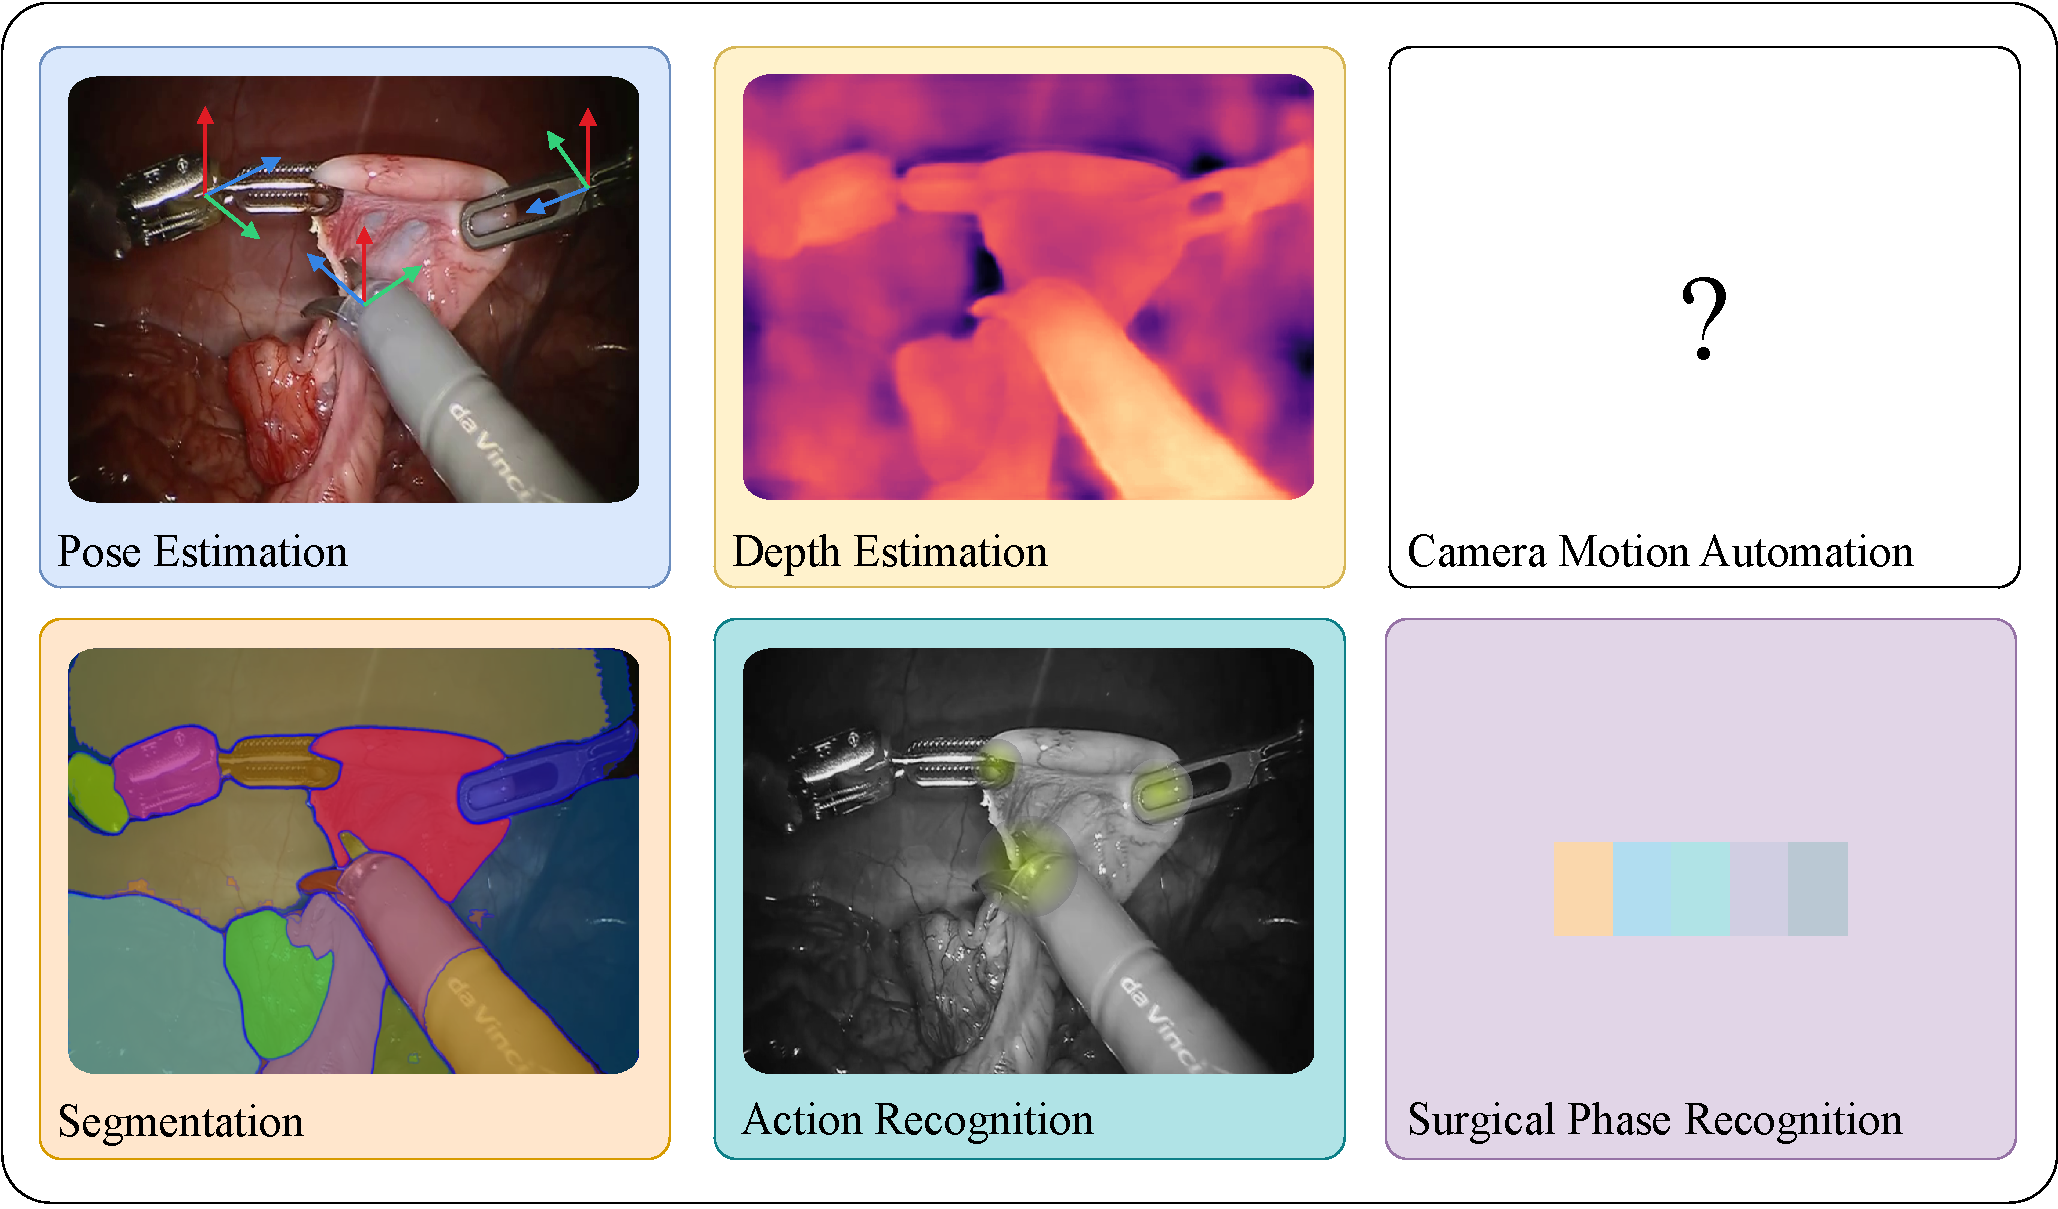
\includegraphics[width=\textwidth]{introduction/fig/auxiliary_tasks.pdf}
    \caption{Auxiliary tasks that could be used for laparoscopic camera automation but that are not used in practise. None of the data-driven methods directly attempts laparoscopic camera motion automation in realistic scenarios. The surgical phases refer e.g. back to \secref{in:sec:cholecystectomy_procedure}. Laparoscopic view shows an image from a da Vinci\textsuperscript{\textregistered} system in the SurgVisDom\cite{zia2021surgical} dataset. Monocular depth estimated using \cite{oquab2023dinov2}, segmentations generated through \cite{segment_anything}. Refers to \secref{in:sec:auxiliary_tasks}.}
    \label{in:fig:auxiliary_tasks}
\end{figure}
Apparently, current visual servos oversimplify the automation task greatly. Only \cite{gruijthuijsen2021autonomous} incorporate neural networks for autonomous instrument tracking. What is generally lacking is an understanding for the surgical scene that could help overcome the simplifications that are currently made for visual servoing. Indeed, there exists plenty of research on solving auxiliary vision tasks through data-driven methods, see \figref{in:fig:auxiliary_tasks}. Some of which, will be highlighted below. 

\paragraph{Automation Related Tasks} Based on progress in segmentation tasks, using deep learning, but also with the prospect of identifying tool tips for automating procedures, a vast body of literature on surgical tool segmentation evolved, including \cite{allan20192017, pakhomov2019deep}, and \cite{garcia2016real, garcia2017toolnet, shvets2018automatic, islam2019real, jin2018tool, sarikaya2017detection, da2019self, attia2017surgical, laina2017concurrent}. Some of these segmentation works help improve surgical tool pose estimation, as was shown in \cite{kurmann2017simultaneous, li2020super, hasan2021detection}, as does monocular depth estimation \cite{li2020unsupervised,huang2021self,xu2022self,li2023multi} and \cite{li2022geometric,bardozzo2022stasis,huang2022simultaneous,huang2022self}. Whilst these works could be fused with any of the visual servos from above, it wouldn't resolve the general assumption that camera motion only results from tool motion. Besides tool segmentation, research exists for surgical phase detection \cite{stauder2014random, lalys2014surgical, jin2016endorcn, dergachyova2016automatic,twinanda2016endonet,malpani2016system, jin2017sv, ross2018exploiting, yengera2018less, funke2018temporal, yu2018learning} as well as \cite{bodenstedt2019active, padoy2019machine, czempiel2020tecno, jin2020multi, kitaguchi2020real}. These could condition visual servos on the current phase of the surgery. Other self-supervised approaches, which could be integrated similarly, aim to estimate the remaining time of a surgical procedure \cite{twinanda2018rsdnet, bodenstedt2019prediction, rivoir2019unsupervised} or perform action recognition \cite{nwoye2021deep}.

\paragraph{The Automation Task} Automation related tasks, as introduced in the previous paragraph, are often treated as prerequisite for autonomy, but could at present only contribute as input to a smarter visual servoing scheme. Given the success of data-driven methods for these auxiliary tasks, it might be reasonable to utilize them for laparoscopic camera motion automation as well. But instead of taking any of the auxiliary tasks as priors, one might consider learning automation directly, too. This is because, firstly, in deep learning, end-to-end approaches have proven to outperform methods that rely on hand-crafted inputs that may seem humanly logical, and, secondly, it is the simplest approach. So instead of extracting redundant information, such as tool tips, surgery phases, depth, or poses first, we suggest that it might make sense to apply data-driven methods to automating laparoscopic camera motion immediately. This sentiment is supported by related fields, where learning policies on vast amounts of data has demonstrated great success with the emergence of complex behaviors, far more complex than the tool following proxy. Interestingly, data-driven laparoscopic camera motion automation is an underexplored field. In spite of the underexploration of data-driven methods for laparosopic camera motion automation, we turn to a broader body of literature, and introduce several learning-based methods in the next sections \secref{in:sec:reinforcement_learning} and \secref{in:sec:imitation_learning}.

% Put differently, why would one have to segment surgical tools first to extract a control policy, instead of immediately inferring the control policy? 

% From an algorithmic perspective, both approaches should be equally demanding tasks, while the latter doesn't constrain the method in its solution. 

% but also apparant that other methods are necessary to .. complex behavior

% Let alone this realization out-rules all visual servoing approaches that rely on tools only as potential candidates for fully automating camera movement in laparoscopic surgery. 

% Extracting camera motion from images is a well studied problem, but not so much in the surgical context, where an extremely dynamic and deformable environment with little texture hardens the task. 

% Therefore, simplifying the problem is crucial. In its simplest form, one can model a surgical scene as a plane, camera motion can hence be described as a homography and recent advances in deep homography estimation have successfully extracted homographies from images with little texture \cite{detone2016deep, erlik2017homography, nguyen2018unsupervised}. These findings were further applied in the surgical realm by Gomes et al. in \cite{gomes2019unsupervised} and by Bano et al. in \cite{bano2020deep}. Bano et al. further refined their findings in \cite{bano2020vessel} by segmenting veins for the registration process. Yet, none of the above methods takes dynamic scenes into consideration. Most recent literature on deep homography estimation demonstrated how deep homography estimation can be applied to dynamic scenery \cite{le2020deep, zhang2019content}.


\subsection{Reinforcement Learning}
\label{in:sec:reinforcement_learning}
\begin{figure}
    \centering
    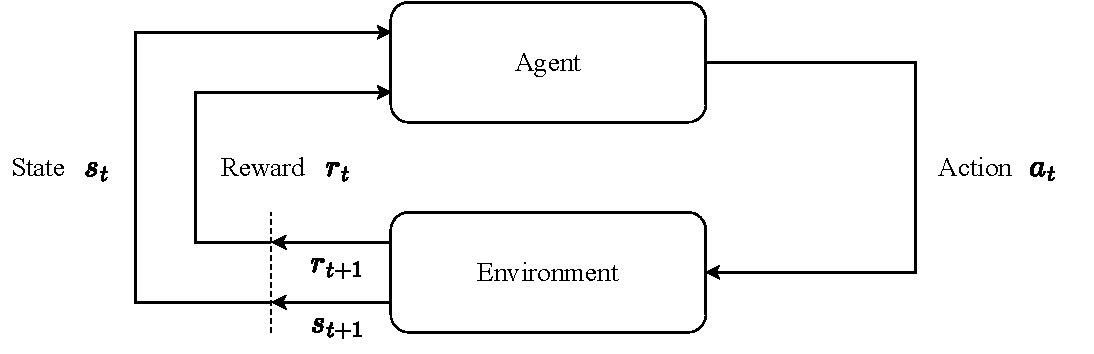
\includegraphics[width=\textwidth]{introduction/fig/reinforcement_learning.pdf}
    \caption{A procedural diagram of reinforcement learning. Given the environment state $s_t$, an agent performs an action $a_t$ and observes the resulting state $s_{t+1}$ and reward $r_{t+1}$. Refers to \secref{in:sec:reinforcement_learning}.}
    \label{in:fig:reinforcement_learning}
\end{figure}
Reinforcement Learning (RL) is conceptually simple and hence so appealing. It, at least in parts, seems to mimic some of the human characteristics for acquiring new skills. In a RL scenario, see \figref{in:fig:reinforcement_learning}, an agent interacts with an environment. The agent observes state $s_t$ and performs an action based on it. The agent will then observe the changed state $s_{t+1}$ and receive a reward $r_{t+1}$. Through trial and error, the agent will try to maximize the reward. RL is sample inefficient and requires a large amount of trials until the agent learns to solve a task successfully. RL is in fact so sample inefficient, that it is often applied to simulation, where physical systems can be mimicked far beyond realtime. If a system can be simulated well, then RL can find impressively complex behaviors in vast state spaces that could not be explored through classical search algorithms. This is why there exists impressive research in RL, where it was e.g. shown that agents can learn to play Atari games just through observing images \cite{mnih2013playing}. This success lead to systems that are capable of beating humans in the game of Go \cite{silver2016mastering}, which was later improved to learn entirely through self-play \cite{silver2017mastering}. For reference, there exist many more possible states in Go than there are atoms in the known universe. These two examples stem from easily simulatable environments (Go and Atari games) without physics. But even in physically more challenging scenarios, it was shown that humanoid walking can be solved through RL \cite{schulman2017proximal}. The transferability from simulation to the real systems, however, was left unsolved. The most recent advancements succeeded in transferring highly complex policies from simulation to real robots, like standing up \cite{rudin2022learning} or parkour \cite{hoeller2023anymal} on the ANYmal quadruped, and playing football on a simplified humanoid robot \cite{liu2022motor}. The state of simulation in surgery will be summarized in the next paragraph.

\paragraph{Laparoscopic Camera Motion Automation}
\begin{figure}[tb]
    \centering
    \begin{subfigure}[b]{0.49\textwidth}
        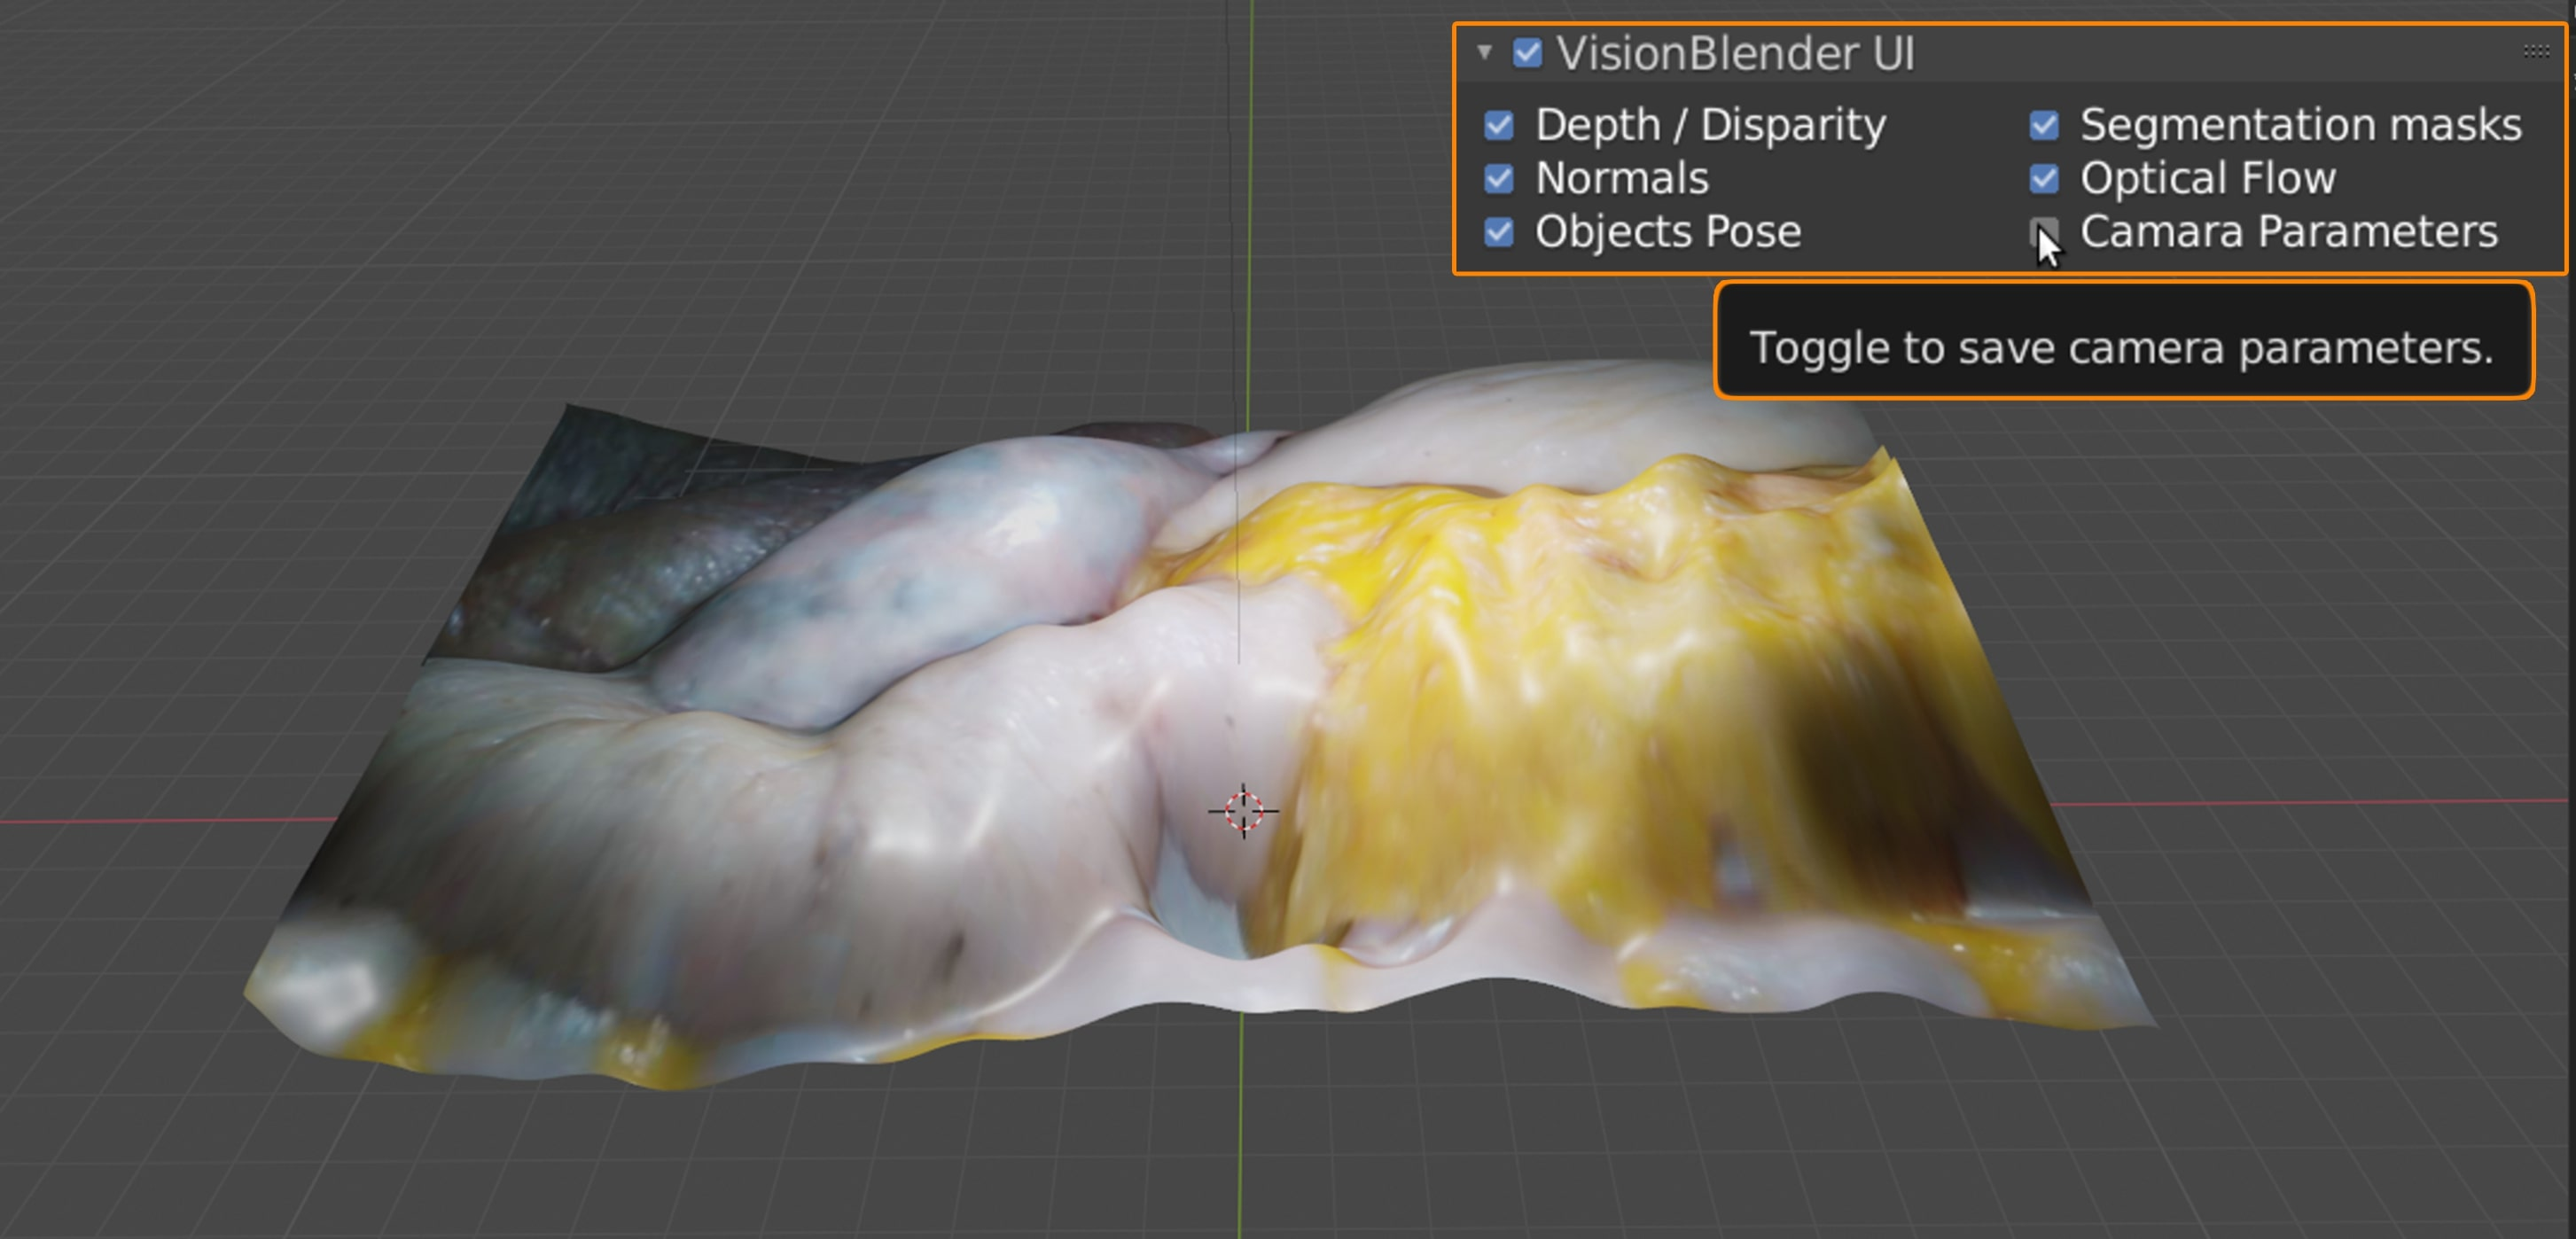
\includegraphics[width=\textwidth]{introduction/img/vision_blender_view.jpg}
        \caption{Static surgical 3D scene.}
    \end{subfigure}
    \begin{subfigure}[b]{0.49\textwidth}
        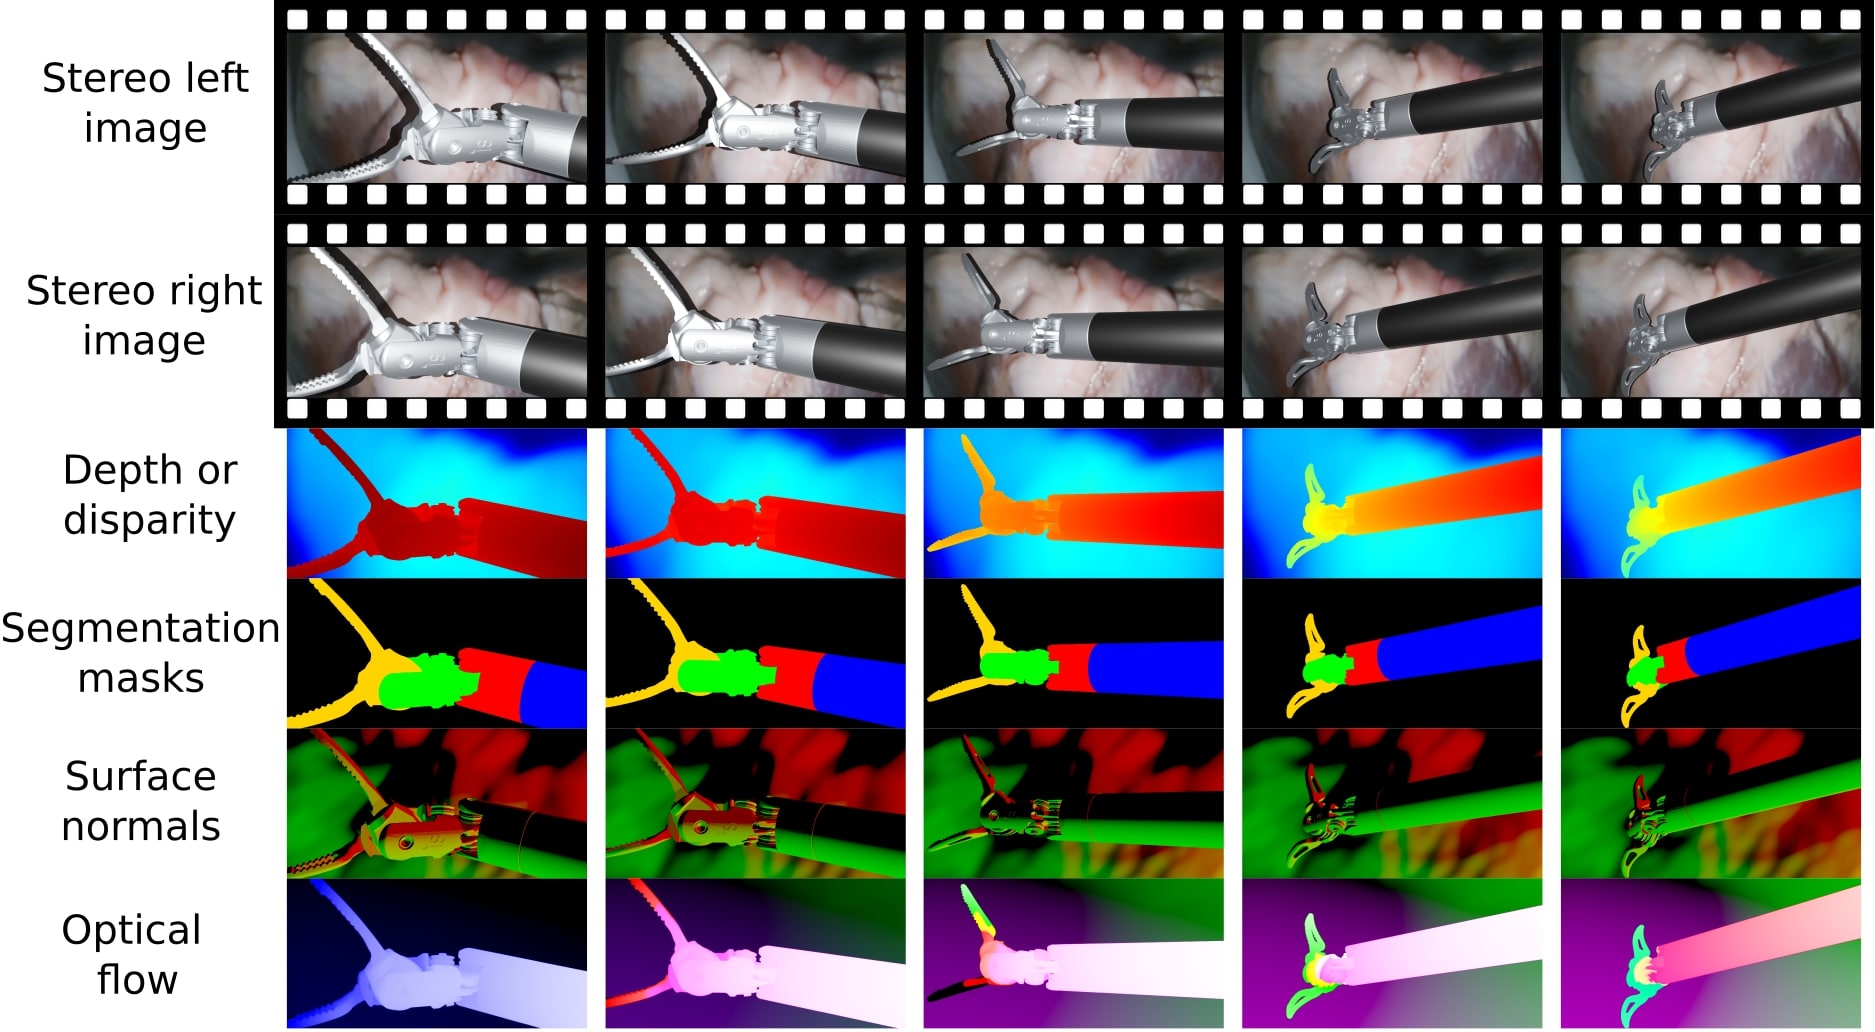
\includegraphics[width=\textwidth]{introduction/img/vision_blender_masks.jpg}
        \caption{Generated masks.}
    \end{subfigure}
    \caption{Blender plugin, named Vision Blender, for rendering realistic surgical scenes. Images with courtesy of \cite{cartucho2021visionblender}. Refers to \secref{in:sec:reinforcement_learning}.}
    \label{in:fig:vision_blender}
\end{figure}
The hurdles for RL in laparoscopic camera motion automation are obvious. The sample inefficiency and potential harm to patients currenty restrict RL approaches to simulation \cite{su2021multicamera,agrawal2018automating}. Significant steps are being made to improve simulations, like \cite{scheikl2023lapgym} using e.g. SOFA \cite{allard2007sofa}, but a domain gap remains. Research that attempts to bridge the domain gap to make RL algorithms deployable in real setups exists, \cite{cartucho2021visionblender} e.g. provide a Blender plugin for realistic view generation, see \figref{in:fig:vision_blender}, and \cite{marzullo2021towards} propose image domain transfer, but only static scenes are considered for now. Clinical translation using RL has yet to be achieved.

We conclude that RL does not comply with the objective of this thesis, that is near term automation that benefits the patient, refer \secref{in:sec:foreword}. This is because simulations have not yet reached the realism that is required for narrowing the domain gap to surgery. Therefore, the next \secref{in:sec:imitation_learning}, will investigate other data-driven methods instead.

\subsection{Imitation Learning}
\label{in:sec:imitation_learning}
The goal of Imitation Learning (IL) is to copy the behavior of an expert demonstrator. Hence, IL aims to extract an expert policy $\pi_\text{E}: s_t \rightarrow a_t$ that maps a state $s_t$ to an action $a_t$, where the actions and states are drawn from a trajectory $\tau_i = \{s_t,a_t...,x_{t+T+1},a_{t+T+1}\}$, sampled from expert demonstrations $\tau_i \in D$. The underlying state $s_t$ might not always be fully observable, in which case one observes $\hat{s}_t = f(s_t)$, where $f$ is the unknown mapping of the underlying state $s_t$ to the observed state $\hat{s}_t$. IL without access to the underlying state is often referred to as Imitation from Observation (IfO) \cite{liu2018imitation}. Also, the embodiment of demonstrator and learner might not always be the same, e.g. if the demonstrator is a human and the learner is a robot, which is called a domain shift. IL is usually achieved via either of two dominant approaches \cite{osa2018algorithmic}: Behavioral Cloning (BC) \cite{pomerleau1991efficient} and Inverse Reinforcement Learning (IRL) \cite{ng2000algorithms}. BC regresses the expert policy $\pi_\text{E}$ from sampled trajectories $\tau_t$ in a supervised fashion. IRL aims to recover the expert's hidden reward $r_t$ to later optimize a policy to also achieve the recovered reward. Neural networks have become the dominant approach for estimating the policy $\pi$, henceforth, the following sections will focus on them.

\subsubsection{Behavioral Cloning}
In a common BC setup that satisfies the Markov property one takes a current state and tries to predict future actions conditioned only on the current state. One can also condition actions on a set of past states \cite{xu2017end} but this is rather uncommon. In \cite{torabi2018behavioral}, Torabi et al. try to perform IfO by randomly exploring the action-state space. They learn a mapping from observations to actions and perform BC on newly obtained observations via this mapping. A general issue in BC is covariate shift, that is the inability to generalize on a small dataset. In \cite{ho2016generative}, Ho et al. address this issue by introducing generative adversarial learning which implicitly regularizes the policy to a bigger action-state space. \cite{torabi2018generative} extends \cite{ho2016generative} by working without immediate access to actions but from observation only. Although generative adversarial imitation learning helps to generalize, a lot of the existing literature focusses on learning an underlying forward dynamics model to infer any policy once the forward dynamics model is known. As such, the authors in \cite{finn2016unsupervised, finn2017deep, nair2017combining} learn to predict future observations from actions via a dataset of randomly explored action-state space trajectories. They use this state transition model to infer actions that lead to desired states, which requires the user to define a desired state. Other attempts to learn arbitrary behaviors are one-shot and zero-shot imitation learning approaches. In one-shot \cite{finn2017one}, Finn et al. use Model-Agnostic Meta-Learning (MAML) to learn how to learn new tasks quickly. Once the network parameters are initialized via meta-learning, a few gradient steps from a demonstration allow to imitate that demonstration. In \cite{yu2018one}, Yu et al. extend this work across domain gaps, that is a robotic learner imitates a human demonstrator from a single demonstration only. Pathak et al. then introduce zero-shot learning in \cite{pathak2018zero}, which introduces a goal conditioned policy, that allows to immediately execute a policy from intermediate pre-defined goal states. In \cite{hausman2017multi}, Hausman et al. extend the work in \cite{ho2016generative} by conditioning the policy on the intention, which similarly to zero-shot imitation learning, allows to reach intermediate goals. The idea of learning a forward dynamics model is then extended into a compressed feature space by Srinivas et al. in Universal Planning Networks \cite{srinivas2018universal}. Their work conditions latent-space dynamics on actions from demonstrations and they define an optimization framework that finds actions conditioned on a goal state. Most recent approaches, such as \cite{lynch2020learning}, learn a latent state representation that categorically clusters different policies as to create interpretable behaviors.


\subsubsection{Inverse Reinforcement Learning}
In IRL the aim is to extract a reward function from a set of expert demonstrations $D$. In practise this can be achieved by embedding observations $\hat{s}_t$ into a meaningful feature space and by enforcing that a newly obtained policy $\pi$ and an expert policy $\pi_\text{E}$ follow similar trajectory embeddings.

Different methods for embedding exist. A triplet loss can be formulated to pull similar images closer to each other while repelling them from different ones. In \cite{wang2014learning, schroff2015facenet}, the authors achieve a triplet loss via a simple distance metric while Wang et al. formulate it as the angle between features \cite{wang2015unsupervised}. Another option is to use prediction as a proxy for meaningful embeddings \cite{vondrick2016anticipating, sermanet2016unsupervised, srivastava2015unsupervised, mathieu2015deep}, self-supervised clustering \cite{caron2018deep}, or, most recently, contrastive learning methods \cite{khosla2020supervised}, which similarly to \cite{wang2015unsupervised} aim to align features of samples with similar properties.

Sermanet et al. in \cite{sermanet2018time} used for example a triplet loss on multi-view videos to learn a view-point invariant embedding that can be used to have a learner learn an expert demonstration. Aytar et al. in \cite{aytar2018playing} had an agent learn to reach checkpoints by sampling checkpoints from demonstrations on YouTube and by defining a reward on the alignment between the current state and the desired checkpoint. In few-shot, Xie et al. \cite{xie2018few} learn initial parameters for a network via MAML, a form of meta-learning, to infer goals in demonstrations from a single gradient-step. They then perform RL to replicate a policy that yields these goals. The idea of Universal Planning Networks by Srinivas et al. in \cite{srinivas2018universal} is further extended by Yu et al. in \cite{yu2019unsupervised}, which learns a goal metric for RL in an unsupervised manner.

\section{Imitation Learning for Laparoscopic Camera Motion Automation}
\label{in:sec:imitation_learning_for_camera_motion_automation}
In the previous sections, several considerations that are relevant to achieving laparoscopic camera motion automation, including economical, clinical, and technical aspects, were introduced. Plenty arguments went into the decision making and some of which may have already been forgotten. Therefore, in this section, we will revisit the key-concepts in \secref{in:sec:revisiting_key_concepts}. Next, and given these critical considerations, we will hypothesize a method for laparoscopic camera motion automation in \secref{in:sec:hypothesizing}, followed by several sections on realizing the hypothesized approach.

\subsection{Revisiting Key Concepts}
\label{in:sec:revisiting_key_concepts}
\paragraph{The Case for Camera Motion Automation} In the Foreword, \secref{in:sec:foreword}, it was argued that the progressive nature of surgery will ultimately alleviate clinical staff of unfulfilling tasks through achieving level five autonomy, likely first for laparoscopic camera motion. We took the clinicians' perspective in the cholecystectomy procedure, the most common laparoscopic procedure, to investigate automation claims further. We found that the camera holder assistant, see \figref{in:fig:room_setup}, performs a relatively simple and unfulfilling task. This stays in contrast with the importance of the camera holder's role of establishing and maintaining a good view for highlighting critical anatomies to surgeons, \secref{in:sec:cholecystectomy_procedure}. We then analyzed the rise of RMIS in \secref{in:sec:the_rise_of_robot_assisted_laparoscopy}, and found first indicators that, in RMIS, the camera is moved more frequently when compared to MIS, suggesting that even more camera motion might be desirable. This stays is in line with the initial rise of RMIS. We thus concluded that camera motion automation might be beneficial for the surgeon, the patient, and the clinical staff in \secref{in:sec:enhancing_current_systems}, \figref{in:fig:advancing_robotic_laparoscopy}.

\paragraph{High-level Aspects of Camera Motion Automation}
\begin{figure}
	\centering
	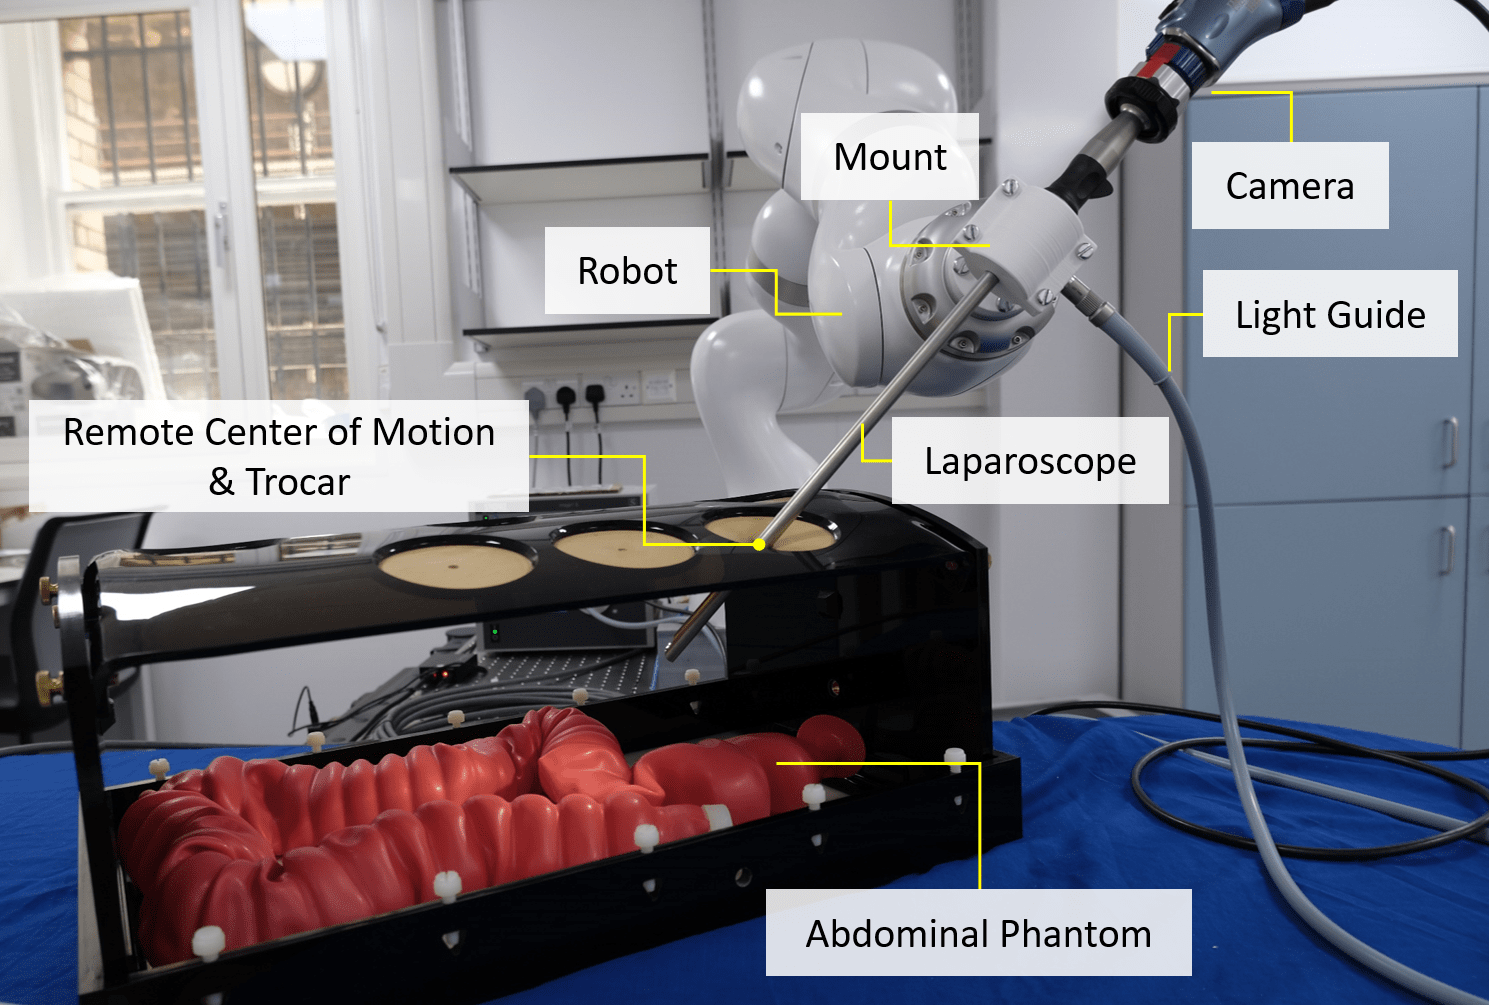
\includegraphics[width=0.8\textwidth]{chapter_2/img/labeled_setup_compressed.png}
	\caption{Robotic setup. A Storz Endocameleon Hopkins Telescope, which provides a light source port and a camera attachment point, is mounted to a KUKA LBR Med 7 R800 robot via a 3D printed clamp. The robotic system undergoes image-based control to reach desired views of the surgical scene and simultaneously pivots around a programmable RCM.}
	\label{in:fig:experimental_setup}
\end{figure}
We took economical considerations into account for propagating the clinically beneficial automation changes to the patients with minimal impact on cost. This resulted in the goal of delivering the automation endeavor through a system with programmable RCM to surgeries that are currently robot-free, \secref{in:sec:automation}. We thus propose a system design that will serve as foundation to this thesis, see \figref{in:fig:experimental_setup}.

Following the clinical prospects of automation and the economically guided form-factor, we analyzed technical factors. We explained calibration prerequisites, \figref{in:fig:eye_in_hand_setup}, \figref{in:fig:com}, and derived novel means of registration for an improved clinical workflow in \secref{in:sec:unified_calibration}, which finally lead to automation itself. We discussed several automation approaches in \secref{in:sec:automation_approaches}, and concluded that learning complex policies, beyond tool following, would require data-driven methods. Crucially, among other reasons, we chose vision as a candidate domain, and thus visual servoing as a candidate for automation, since vision was identified as a shared domain between RMIS and MIS, \figref{in:fig:shared_domain}. We found, however, that vision is currently only used for solving auxiliary tasks, \figref{in:fig:auxiliary_tasks}. We evaluated the state of RL in \secref{in:sec:reinforcement_learning}, and concluded that it does not align with our goals of near term level five autonomy, and were thus left with imitation learning approaches in \secref{in:sec:imitation_learning}. With the robot-free surgery target in mind and the suggested imitation learning as substrate for automation, we impose embodiment-invariance onto the solution. That is, the expert demonstrator can be human, and the executing agent is a robot. Precisely speaking, we are, therefore, trying to solve imitation learning from observation, with only access to the partially observed environment state $\hat{s}_t$. The next sections will go into detail on how this could be achieved.

\subsection{Hypothesizing Embodiment-invariant Laparoscopic Camera Motion Automation}
\label{in:sec:hypothesizing}
\begin{figure}[tb]
    \centering
    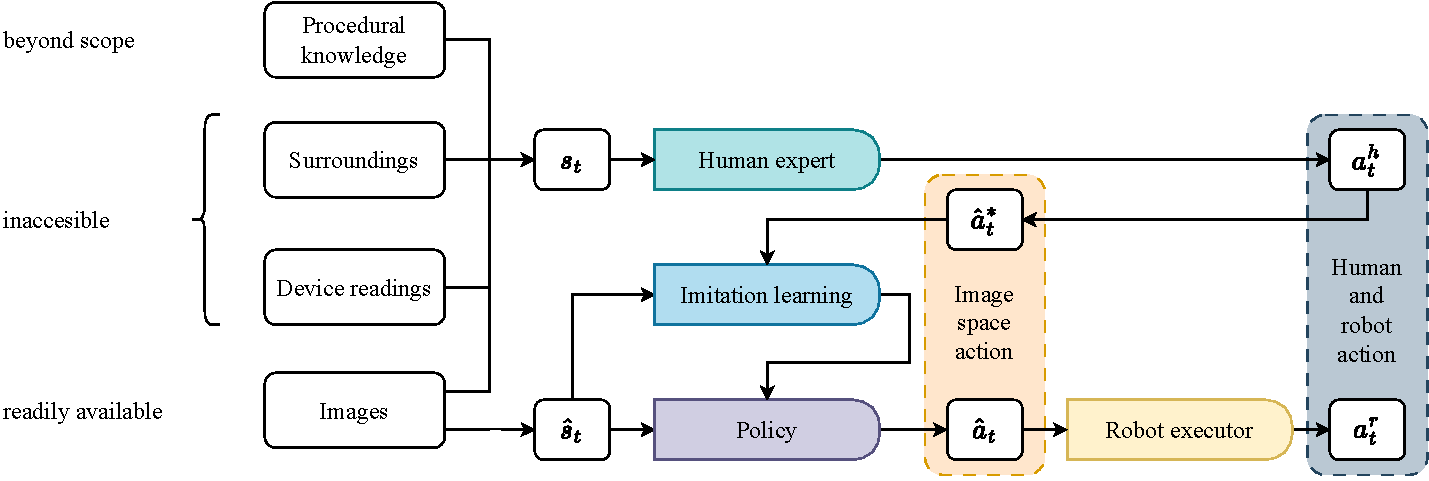
\includegraphics[width=\textwidth]{introduction/fig/camera_motion_action.pdf}
    \caption{The hypothesized approach for laparoscopic camera motion imitation learning. Actions are learned in the shared vision domain and executed via different embodiments, the human or the robot. Refers to \secref{in:sec:hypothesizing}.}
    \label{in:fig:hypothesized_pipeline}
\end{figure}
Having outlined the scope for laparoscopic camera motion automation - embodiment-invariant imitation learning from observation - further referred to simply as imitation learning, this section will now hypothesize concrete means of achieving it. It will dissect the thought process for framing the path towards autonomy in this thesis rigorously.

IL requires large amounts of data for learning the tail-end, i.e. rare cases. Therefore, we will initially search for available data in \secref{in:sec:search_for_available_data}. Given the data, a mixture of supervised and self-supervised methods for learning to predict camera motion, and predicting can be considered imitating, will be suggested in \secref{in:sec:supervised_self_supervised}. Next, a camera motion formulation for the suggested supervised and self-supervised frameworks will be proposed in \secref{in:sec:homography_based_camera_motion_formulation}, keeping the constraint of embodiment-invariance in mind. Finally, \secref{in:sec:robotic_laparoscope_control} will explain classical and clinically applicable methods for controlling a robotic laparoscope under the camera motion prediction.  An overview of the proposed approach is already shown in \figref{in:fig:hypothesized_pipeline}.

\subsubsection{Search for available Data}
\label{in:sec:search_for_available_data}
\begin{table}
\centering
\caption{Exhaustive overview of publicly available MIS and RMIS datasets. All datasets were acquired and analyzed for task-appropriate metrics. Datasets that were not available, or are unreasonable for evaluation, are marked with N/A, where datasets were not available or unreasonable to analyze.}
\label{in:tab:datasets}
\begin{adjustbox}{angle=90, max height=0.9\textheight}
    \begin{tabular}{|c|c|c|r|c|c|c|c|}
        \hline
        \multirow{2}{*}{Collection} & \multicolumn{7}{c|}{Specifications} \\
        \cline{2-8}
        & Name & Year & Length / \# & Frame Rate / Hz & Resolution / pixels & Camera Motion & Note \\
        \hline
        \multirow{8}{*}{\href{https://endovis.grand-challenge.org/}{\shortstack{Endoscopic\\Vision\\Challenge}}} &\href{https://www.synapse.org/#!Synapse:syn21776936/wiki/601700}{MISAW} \cite{mitsuishi2013master}&2020&$128102$&$30$&$460\times 540$&no&synthetic \\
        \cline{2-8}
        &\href{https://surgvisdom.grand-challenge.org/}{SurgVisDom}\cite{zia2021surgical}&2020&$185620$&$20$&$540\times960$&occasional&da Vinci\textsuperscript{\textregistered} \\
        \cline{2-8}
        &\href{https://robustmis2019.grand-challenge.org/}{ROBUST-MIS} \cite{maier2020heidelberg}\cite{ross2020robust}&2019&$7546968$&$25$&$540\times 960$&yes&laparoscopic \\
        \cline{2-8}
        &\href{https://endovissub2019-scared.grand-challenge.org/}{SCARED}&2019&$16818$&$25$&$1024 \times 1280$&yes& exoscopic \\
        \cline{2-8}
        &\href{https://endovissub-workflowandskill.grand-challenge.org/}{SWASA}&2019&N/A&N/A&N/A&yes& laparoscopic\\
        \cline{2-8}
        &\href{https://endovissub2017-workflow.grand-challenge.org/}{SWASA}&2018&N/A&N/A&N/A&yes& laparoscopic\\
        \cline{2-8}
        &\href{https://endovissub2018-roboticscenesegmentation.grand-challenge.org/home/}{RSS} \cite{allan20202018}&2018&$2235$&$2$&$1024\times 1280$&occasional& da Vinci\textsuperscript{\textregistered}\\
        \cline{2-8}
        &\href{https://endovissub2017-roboticinstrumentsegmentation.grand-challenge.org/}{RIS} \cite{allan20192017}&2017&$3225$&$2$&$1024\times 1280$&occasional& da Vinci\textsuperscript{\textregistered} \\
        \cline{2-8}
        &\href{https://endovissub2017-kidneyboundarydetection.grand-challenge.org/}{KBD}&2017&$3000$&$2$&$1024\times 1280$&occasional & da Vinci\textsuperscript{\textregistered}\\
        \cline{2-8}
        &\href{https://endovissub-instrument.grand-challenge.org/}{ISAT}&2015&$16243$&$25$&$480\times 640/576\times 720$& yes & laparoscopic \\
        \hline
        \multirow{3}{*}{\href{http://hamlyn.doc.ic.ac.uk/vision/}{\shortstack{Hamlyn\\Center\\Datasets}}} &\href{http://hamlyn.doc.ic.ac.uk/vision/data/daVinci.zip}{Siamese}\cite{ye2017self}&2017&$34240$&$30$&$192\times 384$& occasional& da Vinci\textsuperscript{\textregistered} \\
        \cline{2-8}
        &Giannarou \href{http://hamlyn.doc.ic.ac.uk/vision/data/Matina/Blur/capture1.avi}{left} / \href{http://hamlyn.doc.ic.ac.uk/vision/data/Matina/Blur/capture2.avi}{right} \cite{giannarou2012probabilistic}&2012&$8063$&$30$&$480\times 640$& occasional& da Vinci\textsuperscript{\textregistered} \\ 
        \cline{2-8}
        &Mountney \href{http://hamlyn.doc.ic.ac.uk/vision/data/Dataset8/left.avi}{left} / \href{http://hamlyn.doc.ic.ac.uk/vision/data/Dataset8/right.avi}{right} \cite{mountney2010three}&2010&$14418$&$30$&$480\times 640$& occasional & da Vinci\textsuperscript{\textregistered}\\
        \hline
        \multirow{4}{*}{Other} &\href{https://www.youtube.com/}{YouTube}&N/A&N/A&N/A&N/A&N/A & N/A \\
        \cline{2-8}
        &\href{https://saras-esad.grand-challenge.org/}{SARAS-ESAD} \cite{bawa2020esad}&2020&$18793$&$1$&$1080\times 1920$& occasional & da Vinci\textsuperscript{\textregistered} \\
        \cline{2-8}
        &\href{http://camma.u-strasbg.fr/datasets}{Cholec80} \cite{twinanda2016endonet}&2017&$4612530$&$25$&$480\times 854$&yes& laparoscopic\\
        \cline{2-8}
        &\href{https://cirl.lcsr.jhu.edu/research/hmm/datasets/jigsaws_release/}{JIGSAW} \cite{ahmidi2017dataset}&2016&$527491$&$30$&$480\times 640$&no& synthetic\\
        \hline
    \end{tabular}
\end{adjustbox}
\end{table}
Given the advancements in deep learning and especially in IL, it is surprising that no one applied IL to automate camera motion in laparoscopic surgery. It appears trivial that camera motion could be learned from data of real surgeries, thereby implicitly tackling the domain-gap that e.g. RL methods face. After having a closer look, it comes, however, at no surprise researchers have not tried. The challenge is to collect sufficient data of high quality. In fact, there exists no dataset with state-action (image-camera motion) pairs. Many works agree and highlight that this lack of expert annotated data hinders progress towards camera motion automation in RMIS \cite{maier2022surgical,kassahun2016surgical,esteva2019guide}.

Data collection is expensive, especially in realistic setups. Recent efforts to make vast amounts of laparoscopic intervention videos publicly available \cite{maier2022surgical} drastically change how IL for camera motion automation could be approached. An overview of the, by the time of this writing, available datasets is shown in \tabref{in:tab:datasets}. The two biggest datasets, by orders of magnitude, are Cholec80 \cite{twinanda2016endonet} and ROBUST-MIS \cite{maier2020heidelberg}, often referred to as Heichole, both are laparoscopic, which is exactly what we are looking for. Some of the datasets, since they come with hand-annotated segmentations, come at low frame rates, i.e. $1-2\,\text{Hz}$, and are, therefore, unusable for IL. As was already pointed out, none of the datasets come with state-action pairs. The only two publicly available datasets that come with kinematic labels are MISAW \cite{mitsuishi2013master} and JIGSAW \cite{ahmidi2017dataset}, but both datasets are captured in synthetic environments and without camera motion.

The missing state-action pairs for all of the available datasets are the major roadblock for applying IL methods to them. Reliably extracting camera motion in retrospect from dynamic surgical scenery is an unsolved task in itself. Somewhat surprisingly, one of the da Vinci\textsuperscript{\textregistered} datasets, SurgVisDom \cite{zia2021surgical}, which was intentionally released for domain transfer, plays an important role in extracting camera motion from laparoscopic videos. How we propose to extract laparoscopic camera motion reliably and how the locking mechanism of the da Vinci\textsuperscript{\textregistered} robot, refer \secref{in:sec:automation}, plays a crucial role, will be explained in the following \secref{in:sec:supervised_self_supervised}.


% with relatively many da vinci videos, althrough still small compared with cholec80 and heichole



% the realization that there exists a da vinci dataset without camera motion
% learning actions from videos of laparoscopic interventions... embodied human -> robot
% bridging the domain gap classically
% lack of camera motion data (prediction paper) -> mock setups



% \begin{itemize}
% 	\item There exists an unknown domain shift between laparoscopic surgery data and the robotic system. This domain shift could be gapped via Reinforcement Learning (RL) on top of IRL, but simple RL in the medical realm puts the patient at risk. We gap this domain shift by finding the greatest common divisor between human demonstrator and robotic learner with a novel optimal control formulation.
% 	\item From the available data, neither the goal state nor the reward function are apparent. Simple BC under a noisy action estimation might be too difficult. To imitate a surgeon demonstrator, a proxy for good views has to be found.\\
% \end{itemize}
% In the following we address how to tackle the first and second challenge. We further identify pathways to solve the third task.





\subsubsection{Supervised and Self-supervised Learning}
\label{in:sec:supervised_self_supervised}
\begin{figure}[tb]
    \centering
    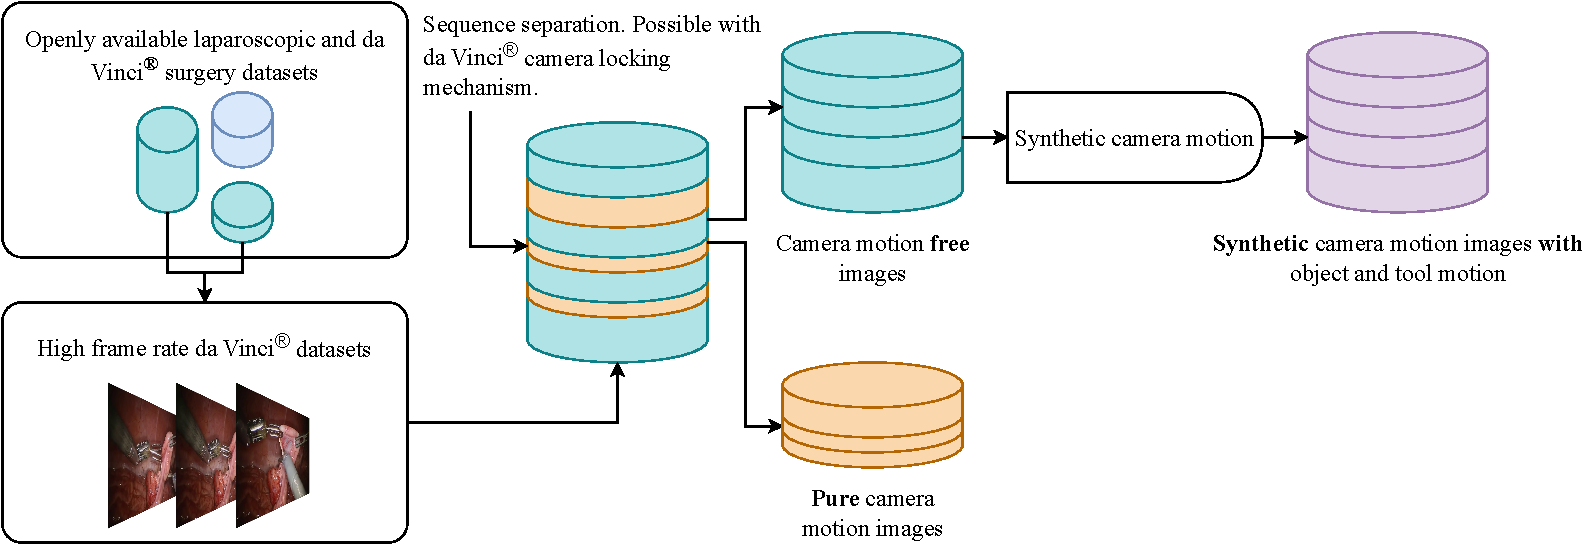
\includegraphics[width=\textwidth]{introduction/fig/camera_motion.pdf}
    \caption{The proposed isolation of camera motion, i.e. actions, and tool as well as object motion. The camera locking mechanism of the da Vinci\textsuperscript{\textregistered} robot allows for extraction of camera motion free image sequences, see \tabref{in:tab:datasets}. Synthetically added camera motion can be used for supervised training. Refers to \secref{in:sec:supervised_self_supervised}.}
    \label{in:fig:camera_motion}
\end{figure}



It is thus not surprising that existing literature on IL for camera motion automation still utilizes data from mock setups \cite{ji2018learning,wagner2021learning}.

As was discussed in \secref{in:sec:auxiliary_tasks}, so far this data is mainly leveraged to solve auxiliary tasks that could at best contribute to camera motion automation. 

For camera motion automation specifically, however, there exist no publicly available
image-action pairs. Some work, therefore, continues to focus on the tools to infer
camera motion [15], or learns on a robotic setup altogether [17] where camera
motion is accessible. The realization, however, that camera motion is intrinsic to
the videos of laparoscopic interventions and that camera motion could be learned
on harvested actions was first realized in [11], and later in [16]. This comes with
the additional advantage that no robot is necessary to learn behaviors and that
one can directly learn from human demonstrations.

%% est:
Non-rule-based, i.e. IL, attempts
that consider both, tissue, and tools as source for camera motion are (Ji et al. 2018;
Su et al. 2020; Wagner et al. 2021), but they utilize an oversimplified setup, require
multiple cameras or tedious annotations

While modern IL approaches could alleviate these issues, clinical
data of laparoscopic surgeries remains unusable for IL. Therefore, SOTA IL attempts
rely on artificially acquired data (Ji et al. 2018; Su et al. 2020; Wagner et al. 2021)





supervised: no camera motion but tool motion, adding synthetic camera motion would allow to learn

self-supervised: learn to predict camera motion on these pseudo labels

\subsubsection{Homography-based Camera Motion Formulation}
\label{in:sec:homography_based_camera_motion_formulation}

introduce all the deep homography estimation

theoretical background homography estimation paper

needs to comply with image + robot

deforemable... assuming the scene is a plane in the first instance, add the text that was writting but commented out above


embodying domain-irrelevant actions
extracting actions
predicting actions

\subsubsection{Robotic Laparoscope Control}
\label{in:sec:robotic_laparoscope_control}
theory of control paper up to merge, i.e. no including merge of two methods

\begin{itemize}
    \item write contributions at beginning of each section
    \item follow why? -> why? -> why? approach to end up at methods
    \item make it an interesting read
    \item write, write, write! hammer it
\end{itemize}


% \subsection{Minimally Invasive Surgery}
% Minimally Invasive Surgery (MIS) minimizes blood loss, allows for faster recovery and leaves a patient with smaller scars. In traditional MIS, a main surgeon would usually be supported by an assistant to help move the endoscope. In this setup, the assistant surgeon often introduces tremor and suffers fatigue. To oveRCMe these, robotic endoscope holders like AESOP \cite{unger1994aesop} or EndoAssist \cite{gilbert2009endoassist} were developed. Different control schemes, such as gaze control, control via joystick, foot or voice were investigated. They, however, lead to eye strain, additional mental workload or communication failures, respectively. Therefore, attempts to automate the endoscope motion via visual servoing were explored. These can broadly by separated into approaches that rely on a mechanical remote center of motion (RCM) and approaches that cast the RCM as part of the optimal control, often referred to as programmable RCM. 




% \subsection{Imitation Learning in this Work}
% Given the advancements in deep learning and especially in IL, it seems surprising that no one applied IL to automate camera motion in laparoscopic surgery. After having a closer look, it comes, however, at no wonder people have not tried. Three major challenges reside:
% \\
% \begin{itemize}
% 	\item IL requires big data, but data collection is expensive, especially in realistic setups. The only two publicly available datasets that come with kinematic labels are MISAW \cite{mitsuishi2013master} and JIGSAW \cite{ahmidi2017dataset}, but both datasets are captured in a synthetic environment and without camera motion. This results in the challenge that all of the available data has no camera motion action labels, and reliably extracting camera motion in retrospect from dynamic surgical scenery is an unsolved task in itself.
% 	\item There exists an unknown domain shift between laparoscopic surgery data and the robotic system. This domain shift could be gapped via Reinforcement Learning (RL) on top of IRL, but simple RL in the medical realm puts the patient at risk. We gap this domain shift by finding the greatest common divisor between human demonstrator and robotic learner with a novel optimal control formulation.
% 	\item From the available data, neither the goal state nor the reward function are apparent. Simple BC under a noisy action estimation might be too difficult. To imitate a surgeon demonstrator, a proxy for good views has to be found.\\
% \end{itemize}
% In the following we address how to tackle the first and second challenge. We further identify pathways to solve the third task.

% \section{METHODS}
% In this section, we first introduce a composite Jacobian gain controller with RCM objective in \secref{in:sec:task_RCM}. We then introduce a homography-based visual servo task for the latter in \secref{in:sec:visual_servo}. Finally, in \secref{in:sec:homography_regression}, we describe different ways of extracting homographies from images.
% \subsection{Task Control with Remote Center of Motion}
% \label{in:sec:task_RCM}
% As derived in \cite{aghakhani2013task}, we update the robot's joint velocities $\dot{\mathbf{q}}$ with a gain controller, following \eqref{in:eq:gain_controller}
% \begin{equation}
% 	\begin{bmatrix}
% 		\dot{\mathbf{q}} \\ 
% 		\dot{\lambda}
% 	\end{bmatrix} =
% 	\mathbf{J}^\#
% 	\begin{bmatrix}
% 		\mathbf{K}_\text{t} & \mathbf{0}_{\text{n}_\text{t} \times 3} \\
% 		\mathbf{0}_{3\times \text{n}_\text{t}} & \mathbf{K}_\text{RCM}
% 	\end{bmatrix}\mathbf{e},
% 	\label{in:eq:gain_controller}
% \end{equation}
% where $\dot{\lambda}$ describes the relative change of the RCM along the endoscope, $\mathbf{J}^\#$ denotes the pseudo-inverse of the composite Jacobian, and $\mathbf{K}_\text{t}$, and $\mathbf{K}_\text{RCM}$ are the gains for the task, and the RCM, respectively. The error $\mathbf{e}$ is defined as
% \begin{equation}
% 	\mathbf{e} = 
% 	\begin{bmatrix}
% 		\mathbf{e}_\text{t} \\
% 		\mathbf{p}_\text{trocar} - \mathbf{p}_\text{RCM}
% 	\end{bmatrix},
% 	\label{in:eq:error}
% \end{equation}
% with the desired trocar position $\mathbf{p}_\text{trocar}$, and the current RCM position $\mathbf{p}_\text{RCM}$ under the relative position $\lambda$. We keep an internal state for the relative position of the RCM $\lambda$ and update it via the desired trocar position $\mathbf{p}_\text{trocar}$ as follows
% \begin{equation}
% \lambda = \frac{(\mathbf{p}_{i+1} - \mathbf{p}_i)^T(\mathbf{p}_\text{trocar}-\mathbf{p}_i)}{\lVert\mathbf{p}_{i+1} - \mathbf{p}_i\rVert_2^2}
% \end{equation}
% Therein, $\mathbf{p}_{i+1}$ denotes the position of the end-effector, which coincides with the camera frame up to orientation and $\mathbf{p}_i$ denotes the joint position prior to the end-effector.
% \subsection{Homography-based Visual Servo Task}
% \label{in:sec:visual_servo}
% As the task error $\mathbf{e}_\text{t}$ in \eqref{in:eq:error}, we use the twist of the camera frame, expressed in the camera frame. Therefore, we rotate the twist from the camera frame to the world frame using $^\textbf{w}\mathbf{R}_\textbf{c}$, as shown below
% \begin{equation}
% 	\mathbf{e}_\text{t} = 
% 	\begin{bmatrix}
% 		^\textbf{w}\mathbf{R}_\textbf{c} & \mathbf{0}_{3\times 3} \\
% 		\mathbf{0}_{3\times 3} & ^\textbf{w}\mathbf{R}_\textbf{c}
% 	\end{bmatrix}
% 	\begin{bmatrix}
% 		\mathbf{e}_{v} \\
% 		\mathbf{e}_\omega
% 	\end{bmatrix}.
% 	\label{in:eq:task}
% \end{equation}
% Following \cite{benhimane2006homography}, we then compute the twist $\begin{bmatrix}\mathbf{e}_v & \mathbf{e}_\omega\end{bmatrix}^T$ from
% \begin{equation}
% 	\begin{split}
% 		\mathbf{e}_v = (\mathbf{H} - \mathbf{I})\mathbf{m}^*\\
% 		[\mathbf{e}_\omega]_\times = \mathbf{H} - \mathbf{H}^T,
% 	\end{split}
% 	\label{in:eq:twist}
% \end{equation}
% where $\mathbf{H}$ is the homography from the desired to the current frame and $\mathbf{m}^*=\begin{bmatrix}
% x^* & y^* & 1
% \end{bmatrix}$ is set as the principal point, hence $\mathbf{m}^* = \mathbf{K}^{-1}\mathbf{p}^*$, with the camera intrinsics $\mathbf{K}$ and $\mathbf{p}^* = \begin{bmatrix}
% u^* & v^* & 1
% \end{bmatrix}$, the principal point in image space.
% \subsection{Homography Regression}
% \label{in:sec:homography_regression}
% Homographies $\mathbf{H}$ express the transformation of points on a plane, which are projected onto normalized coordinates, under rotation and translation of the camera reference frame. Hence one can write
% \begin{equation}
% 	\mathbf{H}\mathbf{m} = \mathbf{m}'
% 	\label{in:eq:homography}
% \end{equation}
% An unknown homography can be found by identifying a set of point correspondences $\{\mathbf{m}_i, \mathbf{m}'_i\}$. By rearranging \eqref{in:eq:homography}, one can define a set of linear equations as follows
% \begin{equation}
% 	\begin{bmatrix}
% 		x_i & y_i & 1 &   0 &   0 & 0 & -x_ix'_i & -y_ix'_i & -x'_i \\
% 		  0 &   0 & 0 & x_i & y_i & 1 & -x_iy'_i & -y_iy'_i & -y'_i
% 	\end{bmatrix}\mathbf{h} = \mathbf{0},
% 	\label{in:eq:homography_linear}
% \end{equation}
% where $\mathbf{h}$ is a column vector holding the entries of $\mathbf{H}$. Since $\mathbf{H}$ is defined up to scale, it has $8$ unknown parameters. Each point $\mathbf{m}_i$ has $2$ variables, it is thus sufficient to find $4$ point correspondences to solve \eqref{in:eq:homography_linear}. Since the points $\mathbf{m}_i$ are usually found in image space $\mathbf{p}_i$, one obtains the projective homography $\mathbf{G}$ by simply solving the equivalent of \eqref{in:eq:homography_linear}. It can be transferred to normalized coordinates via the camera intrinsics $\mathbf{K}$ with
% \begin{equation}
% \mathbf{H} = \mathbf{K}^{-1}\mathbf{G}\mathbf{K}.
% \end{equation}
% A common way to find a set of point correspondences $\{\mathbf{p}_i, \mathbf{p}'_i\}$ in the image space is to find feature descriptors using for example the Scale-invariant Feature Transform (SIFT) \cite{lindeberg2012scale} or Speeded-up Robust Features (SURF) \cite{bay2006surf} and to identify nearest neighbors within the feature descriptors. Another way, subject to more recent research, is to directly learn $\Delta\mathbf{p}_i = \mathbf{p}_i - \mathbf{p}'_i$, the deviation of image edges under a homography transformation, from image space \cite{detone2016deep}. This can be achieved with a neural network, since the homography in \eqref{in:eq:homography_linear} can be differentiated with respect to the set of points $\{\mathbf{p}_i, \mathbf{p}'_i\}$. 
% \subsection{Implementation - Visual Servo with RCM}
% We implement the gain controller from \eqref{in:eq:gain_controller}, as well as the visual servo from \eqref{in:eq:twist}, with the linear algebra library Eigen \cite{guennebaud2010eigen}. Hereby, we obtain the Jacobian matrices in \eqref{in:eq:gain_controller} and the rotations in \eqref{in:eq:task} with the MoveIt library \cite{chitta2012moveit}. To suppress singular forces, we compute the pseudo-inverse of the task Jacobian $\mathbf{J}$ via a damped least-squares solution using the Singular Value Decomposition \cite{buss2004introduction}. To ensure safety, we implement the gain controller as an action server within the Robot Operating System (ROS) \cite{quigley2009ros} that only allows the execution of non-converging joint velocities $\dot{\mathbf{q}}$.
% \subsection{Implementation - Homography Regression}
% \label{in:sec:implementation_homography_regression}
% We synthetically generate image data. Therefore, we randomly augment fog, grayscale, flipping (horizontally and vertically), blurring, brightness and contrast operations.

% \begin{figure}
% 	\centering
% 	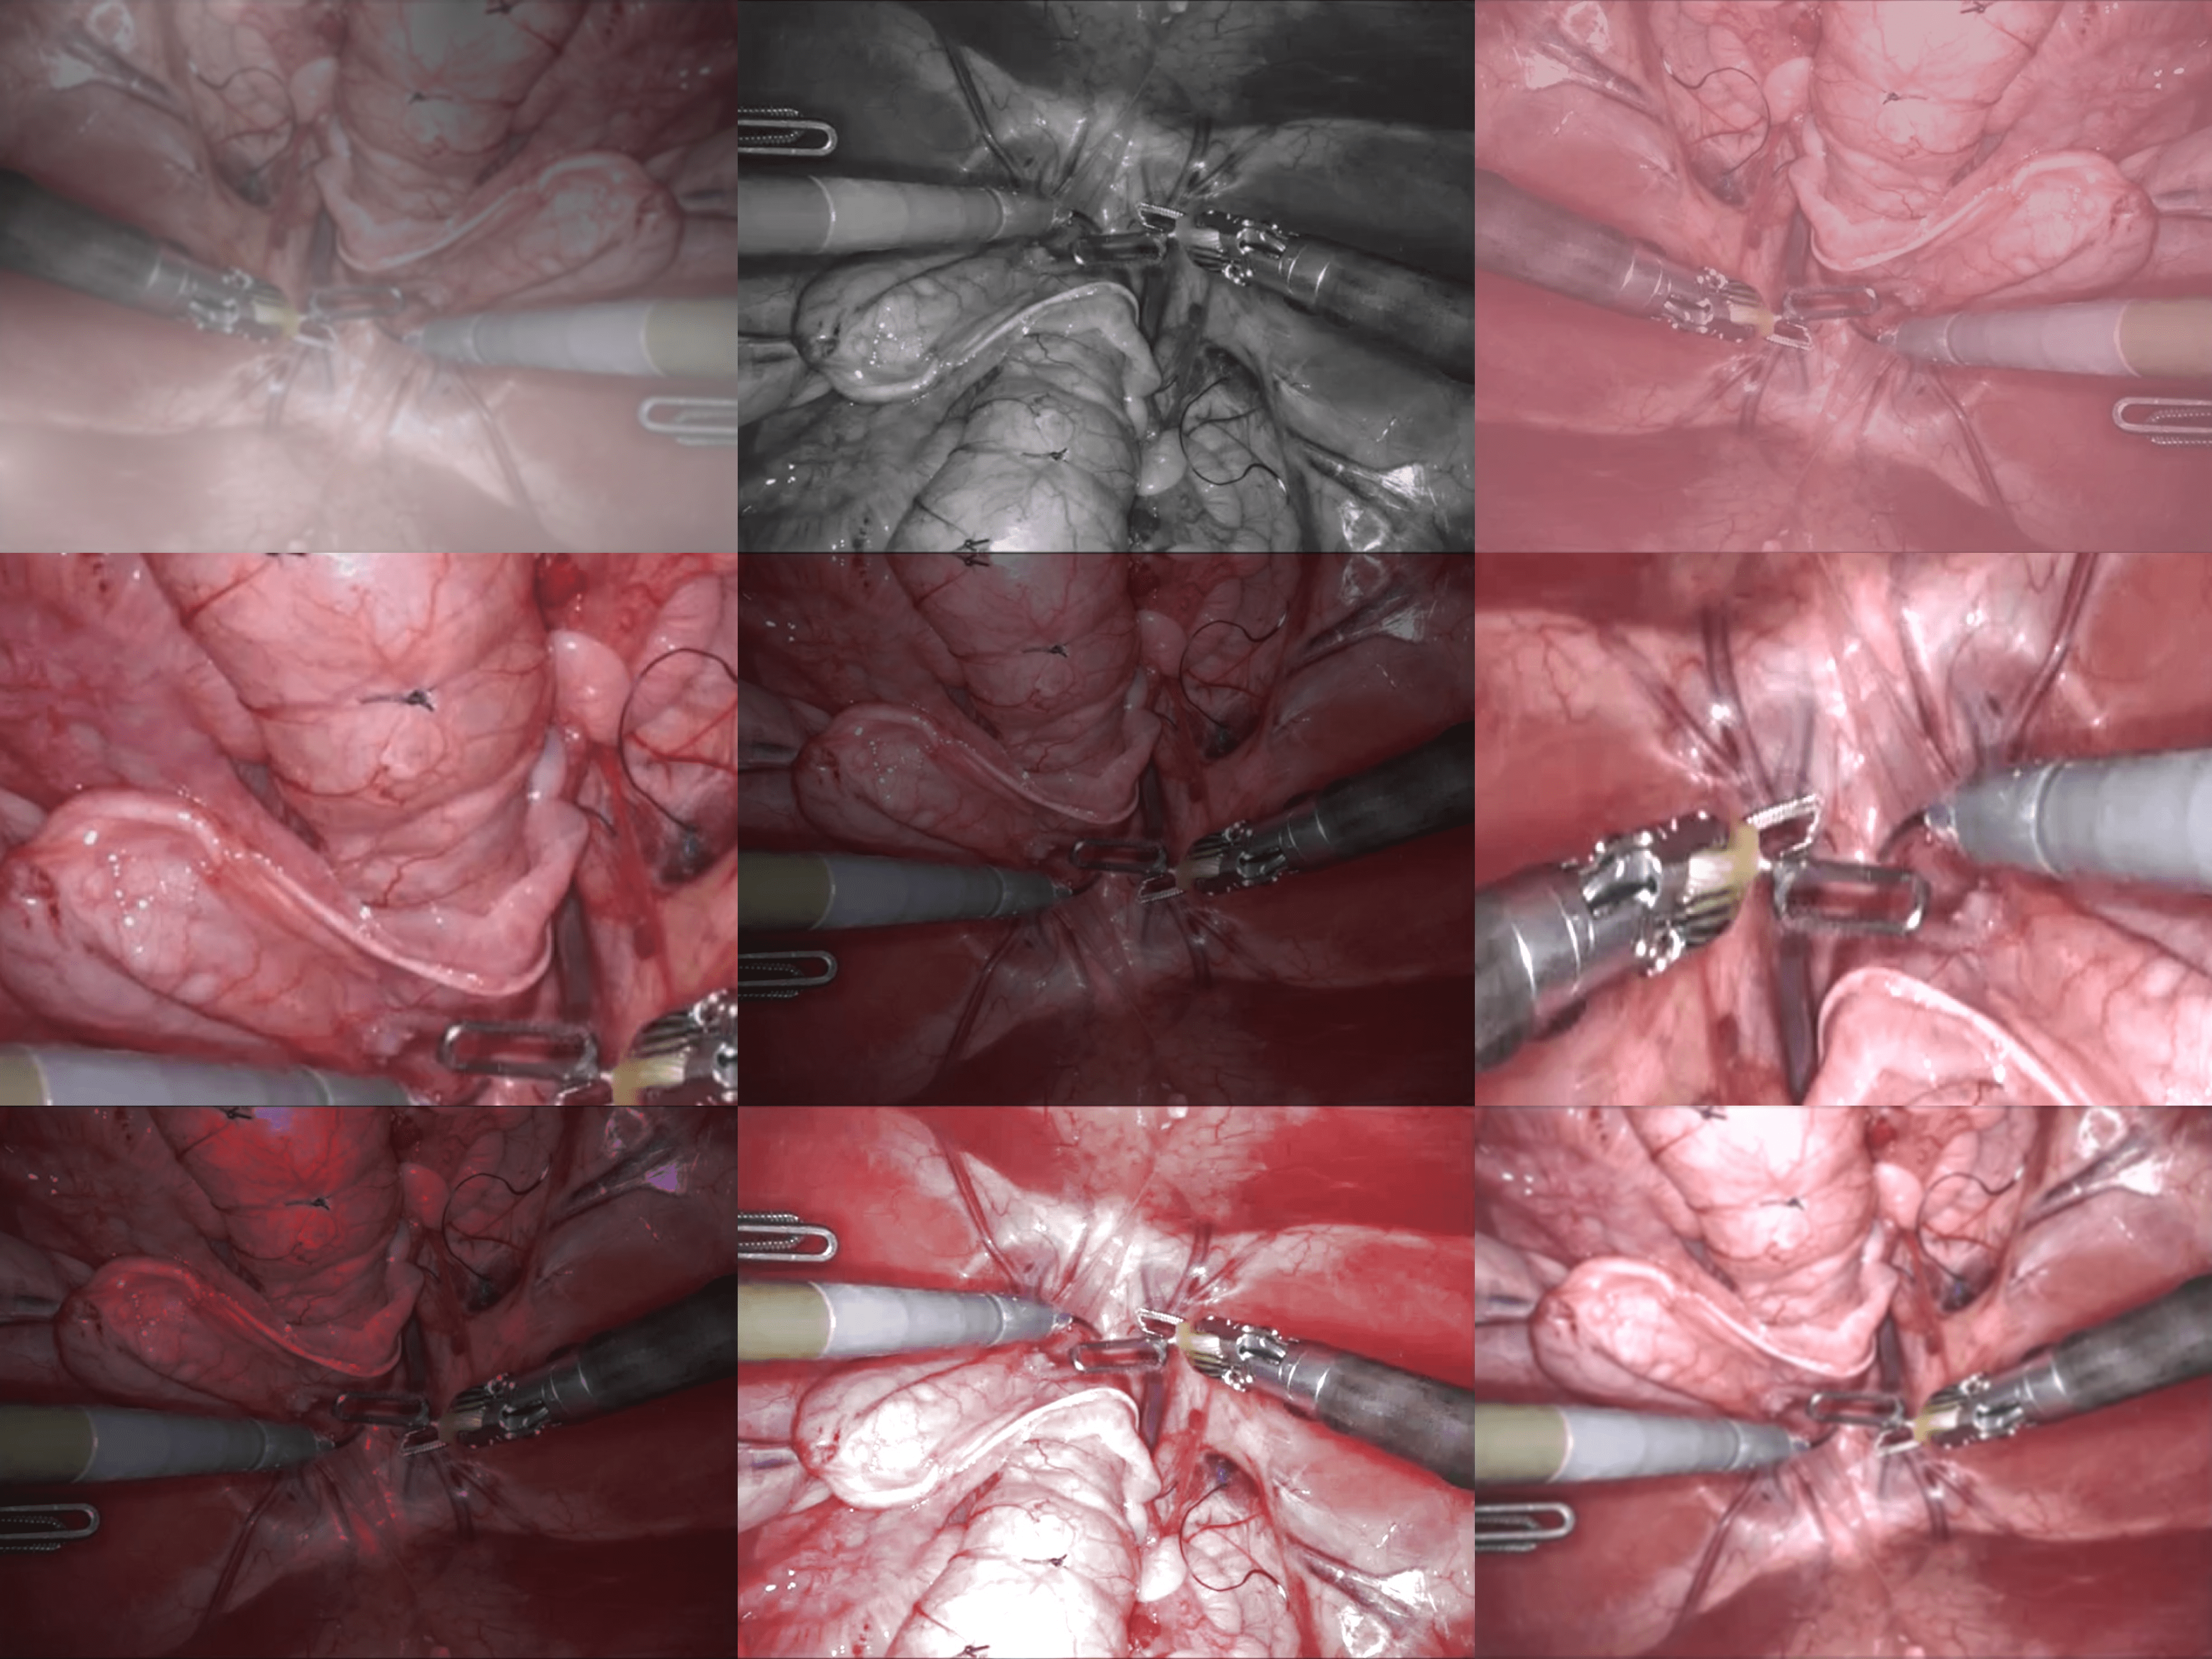
\includegraphics[width=0.8\textwidth]{img/compresspng/augmentations.png}
% 	\caption{Nine different sample variations of the same image from the da Vinci\textsuperscript{\textregistered} SurgVisDom dataset. Shown are random combinations of fog, grayscale, flip, blur, brightness, contrast and crop augmentations.} 	
% 	\label{in:fig:data_augmentation}
% \end{figure}

% As in \cite{detone2016deep}, we then crop the augmented image at edges $\{\mathbf{p}_i\}$, which we then deviate by $\{\Delta \mathbf{p}_i\}$. We apply the corresponding inverse homography to the full image and test whether all points $\{\mathbf{p}_i\}$ still reside within the polygon that is spanned by the new image edges. If so, we keep the sample $\{\mathbf{I}^\text{crop}_t, \mathbf{I}^\text{crop, warp}_{t+1}, \{\Delta\mathbf{p}_i\}\}$ as data point, else we resample $\{\Delta \mathbf{p}_i\}$. To regress $\{\Delta\mathbf{p}_i\}$ in between the sample $\{\mathbf{I}^\text{crop}_t, \mathbf{I}^\text{crop, warp}_{t+N}\}$, we further forward the image pair through a neural network and implement \eqref{in:eq:homography_linear} with the differentiable computer vision library Kornia \cite{riba2020kornia}. As DeTone et al. in \cite{detone2016deep}, we do this in a supervised manner, where we directly regress $\{\Delta\mathbf{p}_i\}$, however, as Nguyen et al. in \cite{nguyen2018unsupervised} and Zhang et al. in \cite{zhang2019content}, we further compute the loss in the image space on the tuple $\{\mathbf{I}^\text{crop}_t, \mathbf{I}^\text{crop, warp}_{t+N}\}$ in an unsupervised approach.
% \subsection{Experimental Setup}
% In our experimental setup, see \figref{in:fig:experimental_setup}, we use a  KUKA LBR Med 7 R800 robot. To control it, we create a bridge to ROS by wrapping the Fast Robot Interface (FRI) \cite{schreiber2010fast} with ROS' Hardware Interface functionality. We mount the laparoscope to the LBR Med 7 robot with a custom designed 3D print. As the laparoscope, we use a Storz 7230 AA Telescope, from which we capture images using a Storz TH 102 H3-Z FI Camera. For illumination, we additionally connect a Storz TL 300 Power LED 300 light source to the laparoscope. The acquired images are sent to the Storz TC 300 Image1 S H3-Link, which links the camera via DP to the Storz TC 200 Image1 S Connect. From there on, the image feed is output to SDI, which we convert to HDMI with a SDI to HDMI converter. We then grab the HDMI signal with a DeckLink 4K Extreme 12G and stream it onto the ROS network.

% \subsection{Data}
% To facilitate imitation learning on laparoscopic surgery data, we extract and isolate camera motion from object motion. Therefore, we collect da Vinci\textsuperscript{\textregistered} surgery data, where the camera only moves occasionally and is mostly fixed in position, but objects are still moving. We isolate data without camera motion from data with camera motion. We additionally collect laparoscopic surgery data with camera motion to imitate it. An exhaustive overview of publicly available datasets is given in \tabref{in:tab:datasets}. We analyze the data for its length, frame rate, resolution and camera motion. We pre-process the laparoscopic data by searching for its center point and bounding circle. We do so by seeking a circle who's radius and center fit best to the edge filtered laparoscopic view with a random sample consensus (RANSAC) \cite{fischler1981random}, see \figref{in:fig:ransac_circle}.

% \begin{figure}
% 	\centering
% 	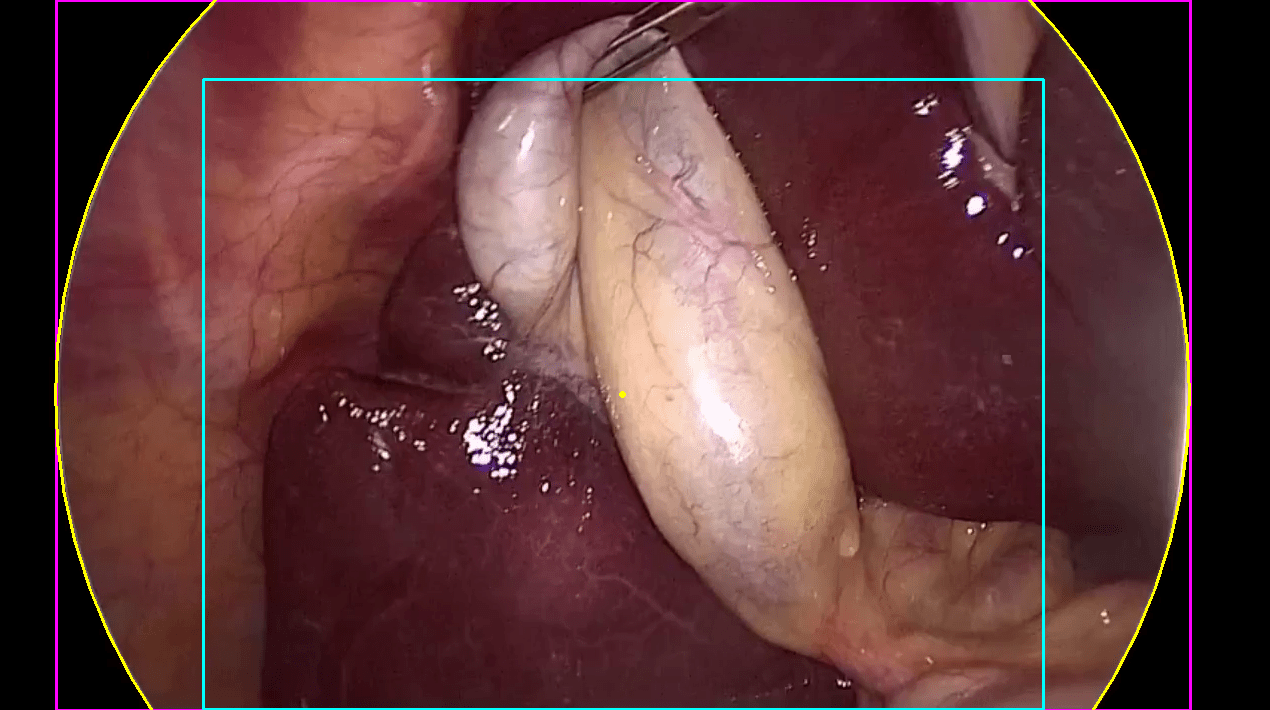
\includegraphics[width=0.8\textwidth]{img/compresspng/ransac_0.png}
% 	\caption{RANSAC detection of the circular boundary of the laparoscopic image from Cholec80 \cite{twinanda2016endonet} (yellow). The turquoise rectangle is the maximum sized rectangle of a given aspect ratio that fits around the circle's center point. An example \href{https://drive.google.com/file/d/1aY7jnBoKNwKyMlSthjzgsRldkHEK1OKw/view?usp=sharing}{video} is provided.}
% 	\label{in:fig:ransac_circle}
% \end{figure}

% \begin{landscape}
% \begin{table}
% \centering
% \caption{Exhaustive overview of publicly available MIS datasets. All datasets were acquired and analyzed for task-appropriate metrics. in:tab:datasetsMetrics were marked with N/A, where datasets were not available or unreasonable to analyze.}
% \label{in:tab:datasets}
%     \begin{tabular}{|c|c|c|r|c|c|c|c|}
%         \hline
%         \multirow{2}{*}{Collection} & \multicolumn{7}{c|}{Specifications} \\
%         \cline{2-8}
%         & Name & Year & Length / \# & Frame Rate / Hz & Resolution / pixels & Camera Motion & Note \\
%         \hline
%         \multirow{8}{*}{\href{https://endovis.grand-challenge.org/}{\shortstack{Endoscopic\\Vision\\Challenge}}} &\href{https://www.synapse.org/#!Synapse:syn21776936/wiki/601700}{MISAW} \cite{mitsuishi2013master}&2020&$128102$&$30$&$460\times 540$&no&synthetic \\
%         \cline{2-8}
%         &\href{https://surgvisdom.grand-challenge.org/}{SurgVisDom}\cite{zia2021surgical}&2020&$185620$&$20$&$540\times960$&occasional&da Vinci\textsuperscript{\textregistered} \\
%         \cline{2-8}
%         &\href{https://robustmis2019.grand-challenge.org/}{ROBUST-MIS} \cite{maier2020heidelberg}\cite{ross2020robust}&2019&$7546968$&$25$&$540\times 960$&yes&laparoscopic \\
%         \cline{2-8}
%         &\href{https://endovissub2019-scared.grand-challenge.org/}{SCARED}&2019&$16818$&$25$&$1024 \times 1280$&yes& exoscopic \\
%         \cline{2-8}
%         &\href{https://endovissub-workflowandskill.grand-challenge.org/}{SWASA}&2019&N/A&N/A&N/A&yes& laparoscopic\\
%         \cline{2-8}
%         &\href{https://endovissub2017-workflow.grand-challenge.org/}{SWASA}&2018&N/A&N/A&N/A&yes& laparoscopic\\
%         \cline{2-8}
%         &\href{https://endovissub2018-roboticscenesegmentation.grand-challenge.org/home/}{RSS} \cite{allan20202018}&2018&$2235$&$2$&$1024\times 1280$&occasional& da Vinci\textsuperscript{\textregistered}\\
%         \cline{2-8}
%         &\href{https://endovissub2017-roboticinstrumentsegmentation.grand-challenge.org/}{RIS} \cite{allan20192017}&2017&$3225$&$2$&$1024\times 1280$&occasional& da Vinci\textsuperscript{\textregistered} \\
%         \cline{2-8}
%         &\href{https://endovissub2017-kidneyboundarydetection.grand-challenge.org/}{KBD}&2017&$3000$&$2$&$1024\times 1280$&occasional & da Vinci\textsuperscript{\textregistered}\\
%         \cline{2-8}
%         &\href{https://endovissub-instrument.grand-challenge.org/}{ISAT}&2015&$16243$&$25$&$480\times 640/576\times 720$& yes & laparoscopic \\
%         \hline
%         \multirow{3}{*}{\href{http://hamlyn.doc.ic.ac.uk/vision/}{\shortstack{Hamlyn\\Center\\Datasets}}} &\href{http://hamlyn.doc.ic.ac.uk/vision/data/daVinci.zip}{Siamese}\cite{ye2017self}&2017&$34240$&$30$&$192\times 384$& occasional& da Vinci\textsuperscript{\textregistered} \\
%         \cline{2-8}
%         &Giannarou \href{http://hamlyn.doc.ic.ac.uk/vision/data/Matina/Blur/capture1.avi}{left} / \href{http://hamlyn.doc.ic.ac.uk/vision/data/Matina/Blur/capture2.avi}{right} \cite{giannarou2012probabilistic}&2012&$8063$&$30$&$480\times 640$& occasional& da Vinci\textsuperscript{\textregistered} \\ 
%         \cline{2-8}
%         &Mountney \href{http://hamlyn.doc.ic.ac.uk/vision/data/Dataset8/left.avi}{left} / \href{http://hamlyn.doc.ic.ac.uk/vision/data/Dataset8/right.avi}{right} \cite{mountney2010three}&2010&$14418$&$30$&$480\times 640$& occasional & da Vinci\textsuperscript{\textregistered}\\
%         \hline
%         \multirow{4}{*}{Other} &\href{https://www.youtube.com/}{YouTube}&N/A&N/A&N/A&N/A&N/A & N/A \\
%         \cline{2-8}
%         &\href{https://saras-esad.grand-challenge.org/}{SARAS-ESAD} \cite{bawa2020esad}&2020&$18793$&$1$&$1080\times 1920$& occasional & da Vinci\textsuperscript{\textregistered} \\
%         \cline{2-8}
%         &\href{http://camma.u-strasbg.fr/datasets}{Cholec80} \cite{twinanda2016endonet}&2017&$4612530$&$25$&$480\times 854$&yes& laparoscopic\\
%         \cline{2-8}
%         &\href{https://cirl.lcsr.jhu.edu/research/hmm/datasets/jigsaws_release/}{JIGSAW} \cite{ahmidi2017dataset}&2016&$527491$&$30$&$480\times 640$&no& synthetic\\
%         \hline
%     \end{tabular}
% \end{table}
% \end{landscape}

% \section{RESULTS}
% In this section we first present and evaluate results for the visual servo in simulation in \secref{in:sec:results_visual_servo} and following that we analyze the homography regression performance in \secref{in:sec:results_homography_regression}. Finally, we measure the homography regression performance qualitatively in a dynamic surgical scene from a previously unseen dataset in \secref{in:sec:homography_imitation_learning}
% \subsection{Homography-based Visual Servo with RCM Objective}
% \label{in:sec:results_visual_servo}
% To demonstrate the effectiveness of the proposed visual servo, we implement an example, where the desired homography $\mathbf{H}$ is computed as a least squares solution with OpenCV's \textit{findHomography} function \cite{bradski2000opencv}. We extract key points from a calibration pattern, perturb the endoscope's position randomly and then iterate \eqref{in:eq:gain_controller} to minimize the task error $\mathbf{e}_\text{t}$ in \eqref{in:eq:error}, which is supposed to move the endoscope to the initial position. We set the task gain parameters $\mathbf{K}_\text{t} = \text{diag}(1.0,1.0,1.0,0.04,0.04,0.04)$ and the RCM gain parameters $\mathbf{K}_\text{RCM} = \text{diag}(100.0, 100.0, 100.0)$. We set the damping factor for the damped least squares inverse of the Jacobian matrix to $\gamma = 0.05$.
% An exemplary \href{https://drive.google.com/file/d/1xrPTe7FdxZiUFySA3CxLsW-lJGgMdrcS/view?usp=sharing}{video} is available on Google Drive. We evaluated the convergence of the task error $\mathbf{e}_\text{t}$, the deviation of the RCM $\mathbf{p}_\text{RCM}$ from the desired trocar position $\mathbf{p}_\text{trocar}$, as well as a visual error that we define as the mean pairwise distance of the key points found on the calibration board and the deviation of the tip position from the initial pose. Results are shown in \figref{in:fig:visual_servo_measurements}.

% \begin{figure}
% 	\centering
% 	\begin{subfigure}[b]{.4\textwidth}
% 		\centering
% 		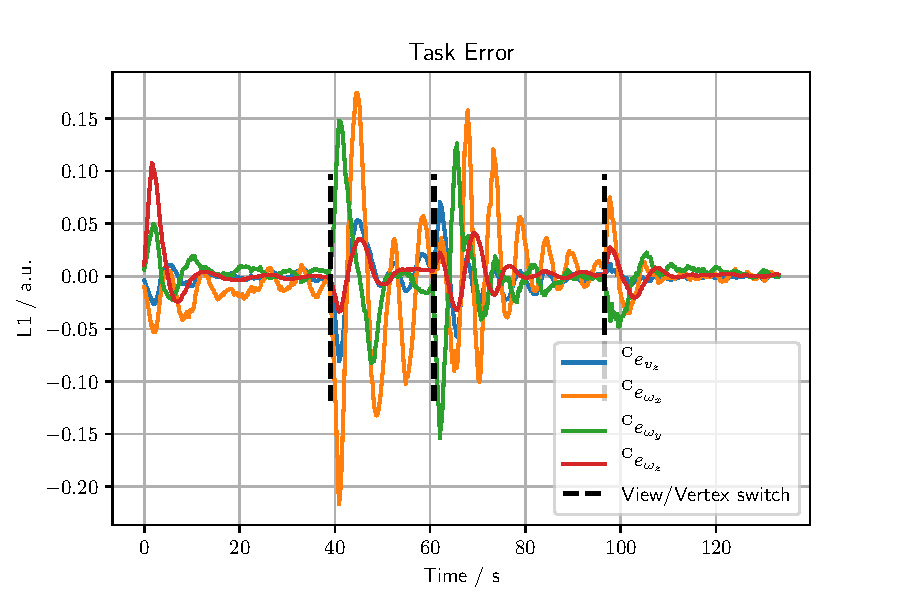
\includegraphics[width=1.0\textwidth]{fig/task_error.pdf}
% 		\caption{Task error over time, refer to \eqref{in:eq:task}. The task, as computed from the desired homography, converges.}
% 	\end{subfigure}\hspace{2em}
% 	\begin{subfigure}[b]{.4\textwidth}
% 		\centering
% 		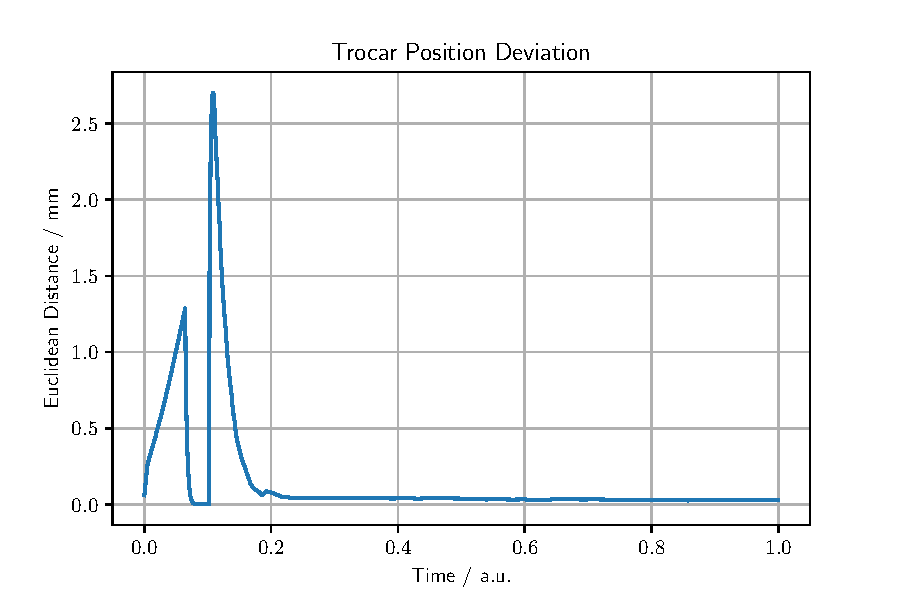
\includegraphics[width=1.0\textwidth]{fig/trocar_position_deviation.pdf}
% 		\caption{Trocar position deviation over time, refer to \eqref{in:eq:error}. The deviation stays below a couple of millimeters under task motion and converges again.}
% 	\end{subfigure}
% 	\begin{subfigure}[b]{.4\textwidth}
% 		\centering
% 		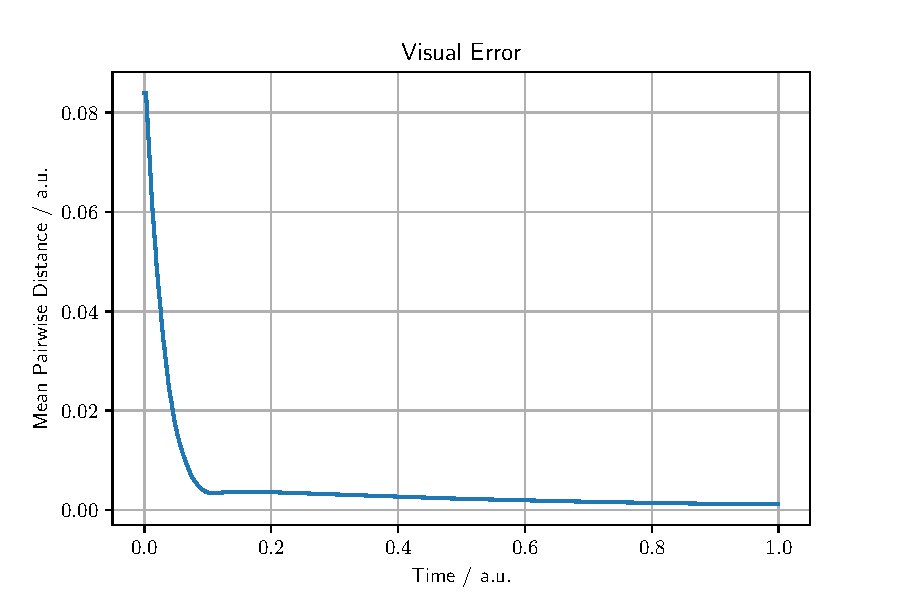
\includegraphics[width=1.0\textwidth]{fig/visual_error.pdf}
% 		\caption{The mean pairwise distance of calibration plane points in the normalized image plane converges.}
% 	\end{subfigure}\hspace{2em}
% 	\begin{subfigure}[b]{.4\textwidth}
% 		\centering
% 		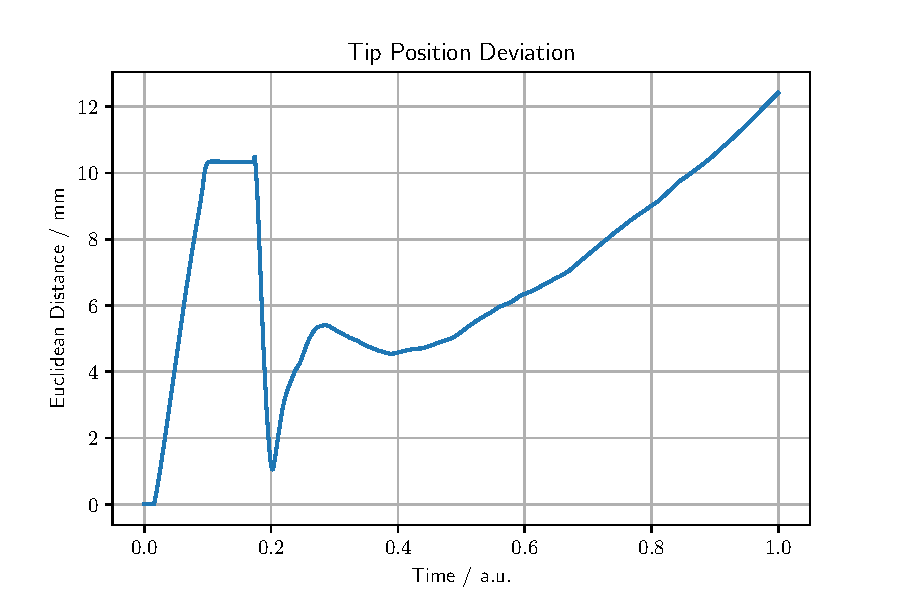
\includegraphics[width=1.0\textwidth]{fig/tip_position_deviation.pdf}
% 		\caption{The tip position is first changed on purpose, then converges to close to zero after the visual servo is initialized but then starts to diverge, although the task errors are being minimized.}
% 	\end{subfigure}
% 	\caption{Evolution of different errors over time. In the setup, we perturb the laparoscope's tip and then initialize the homography-based visual servo to return to the initial position. Results were obtained in simulation.}
% 	\label{in:fig:visual_servo_measurements}
% \end{figure}

% \subsection{Homography Regression}
% \label{in:sec:results_homography_regression}
% As visualized in \figref{in:fig:datasets_sizes}, the datasets SurgVisDom, Giannarou and Mountney account for $72.4\%$ of data with occasional camera motion. 

% \begin{figure}
% 	\centering
% 	\begin{subfigure}[b]{.45\textwidth}
% 		\centering
% 		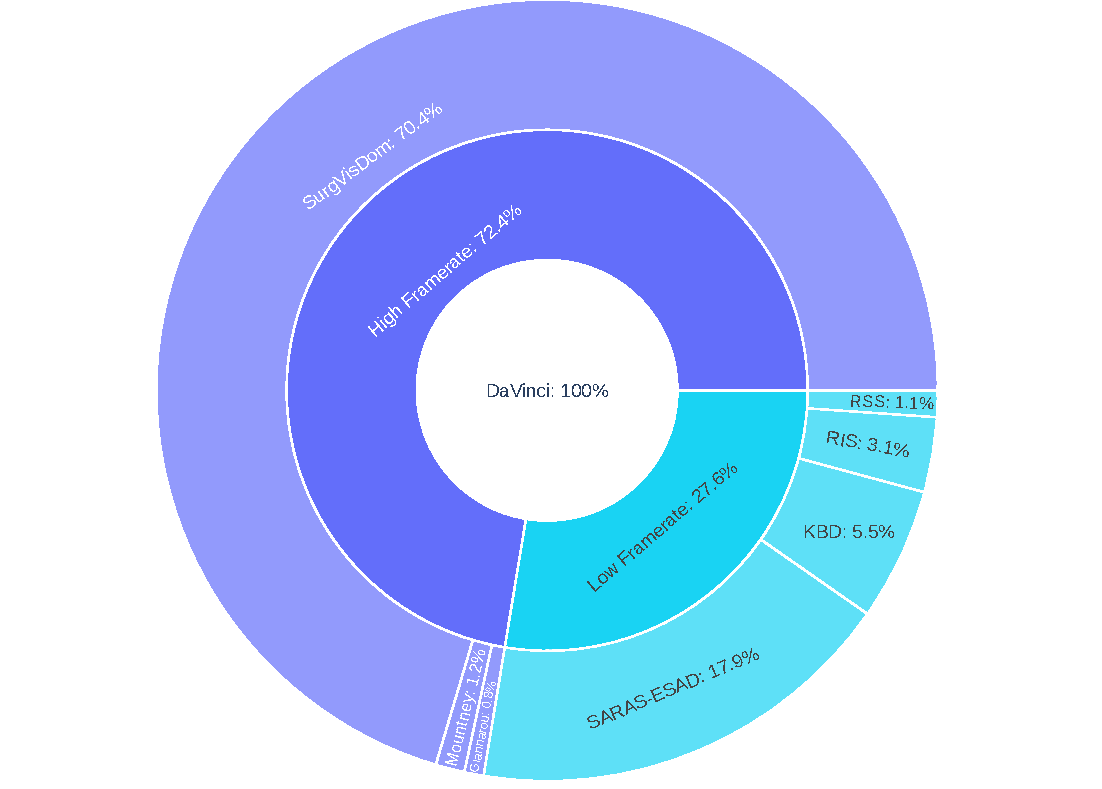
\includegraphics[width=1.\linewidth]{fig/fig_da_vinci.pdf}
% 		\caption{da Vinci\textsuperscript{\textregistered} surgery datasets modulo the Siamese dataset due to low resolution. The high frame rate datasets naturally cover $72.4\%$ of available data.}
% 		\label{in:fig:da_vinci}
% 	\end{subfigure}\hspace{2em}
% 	\begin{subfigure}[b]{.45\textwidth}
% 		\centering
% 		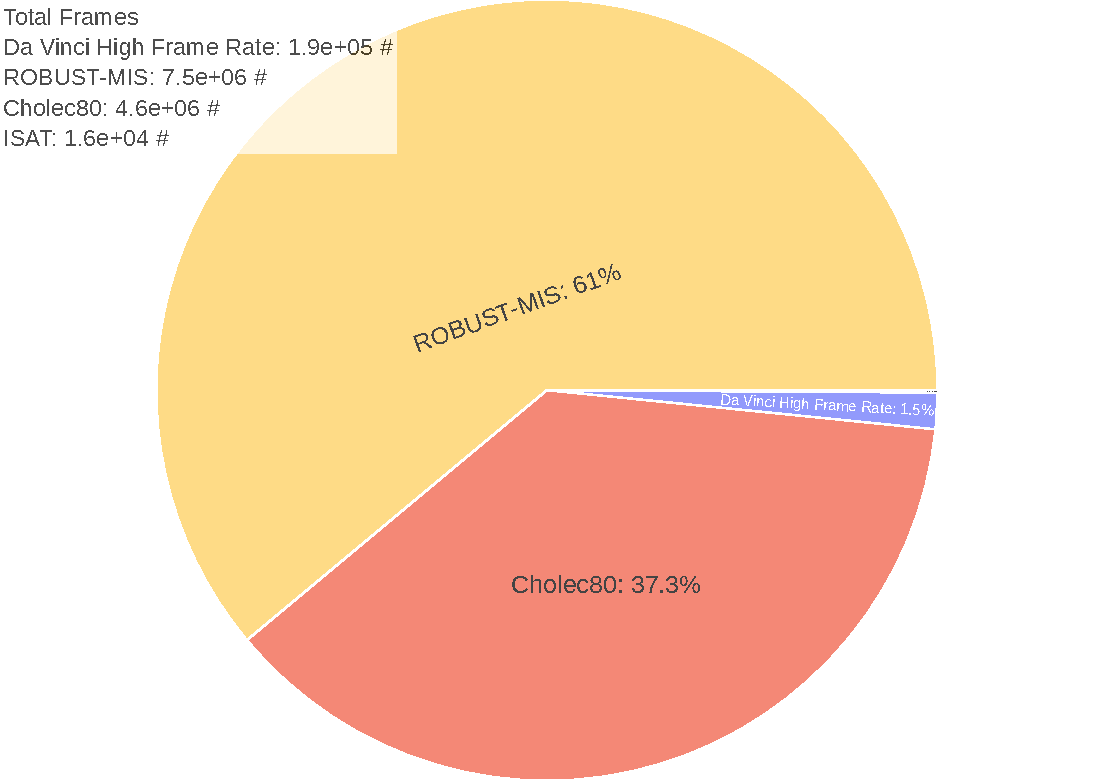
\includegraphics[width=1.\linewidth]{fig/fig_da_vinci_high_fps_laparoscopic.pdf}
% 		\caption{Laparoscopic datasets and a concatenation of the da Vinci\textsuperscript{\textregistered} high frame rate datasets. The ISAT dataset can barely be seen in this visualization. The Cholec80 dataset corresponds to about $51\,\text{h}$ of video.}
% 		\label{in:fig:da_vinci_laparoscopic}
% 	\end{subfigure}
% 	\caption{Dataset length visualizations for datasets listed in \tabref{in:tab:datasets}. Shown is the fraction of total number of images within a dataset.}
% 	\label{in:fig:datasets_sizes}
% \end{figure}

% $95\%$ of this data has no camera motion. We train all approaches from \secref{in:sec:implementation_homography_regression} on this data. We augment data with following probability
% \begin{itemize}
% 	\item Grayscale: $10\%$
% 	\item Horizontal flip: $50\%$
% 	\item Vertical flip: $50\%$
% 	\item Crop: $20\%$
% 	\item Brightness: $30\%$
% 	\item Gaussian blue: $10\%$
% 	\item Fog: $10\%$
% 	\item Contrast: $20\%$
% \end{itemize}
% Example augmentations are shown in \figref{in:fig:data_augmentation}. We train VGG-based networks and networks with a Resnet34 \cite{he2016deep} backbone. We use the Adam optimizer at a learning rate of $1\mathrm{e}{-4}$ and a momentum of $[0.9, 0.999]$. We set the batch size to $64$, the image crop shape to $480\times640$ and train for $20$ epochs on a train split with $80\%$ of the total data. The results are shown in \tabref{in:tab:train_results}. We excluded the results for the method from \cite{zhang2019content}, as it converged to the trivial solution.
% \begin{table}
% 	\centering
% 	\caption{Test loss on high frame rate da Vinci\textsuperscript{\textregistered} dataset without camera motion.}
% 	\begin{tabular}{ccc}
% 		Architecture & Supervised & Mean Pairwise Distance / pixels\\
% 		\hline
% 		VGG \cite{detone2016deep}         & yes & $4.547$ \\
% 		VGG \cite{nguyen2018unsupervised} & no  & $5.875$ \\
% 		Resnet34                          & yes & $\mathbf{1.566}$ \\
% 		Resnet34                          & no  & $2.944$	
% 	\end{tabular}
% 	\label{in:tab:train_results}
% \end{table}
% The Resnet34-backboned network performs the best.
% \subsection{Homography Imitation Learning}
% \label{in:sec:homography_imitation_learning}
% To qualitatively assess the homography estimation capability of the Resnet34-backboned network, we perform inference on the unseen Cholec80 dataset. We do so as the Cholec80 dataset accounts for about $37\%$ of available laparoscopic data, see \figref{in:fig:da_vinci_laparoscopic}, and consists of continuous video, whereas the ROBUST-MIS dataset only comprises short video clips of length $10\,\text{s}$. We compare the deep method against a SIFT feature-based homography estimation method. Exemplary alpha blends are shown in \figref{in:fig:alpha_blend}. Example videos of the alignment with \href{https://drive.google.com/file/d/1SpUtSVgwo_PAwAjULF-Ky_5CxRuhMYlm/view?usp=sharing}{stride 1} and \href{https://drive.google.com/file/d/17fmhSsPq290PuLXmtO-aWwo3KN4QkZA8/view?usp=sharing}{stride 10} are also provided on Google Drive.

% \begin{figure}
% 	\centering
% 	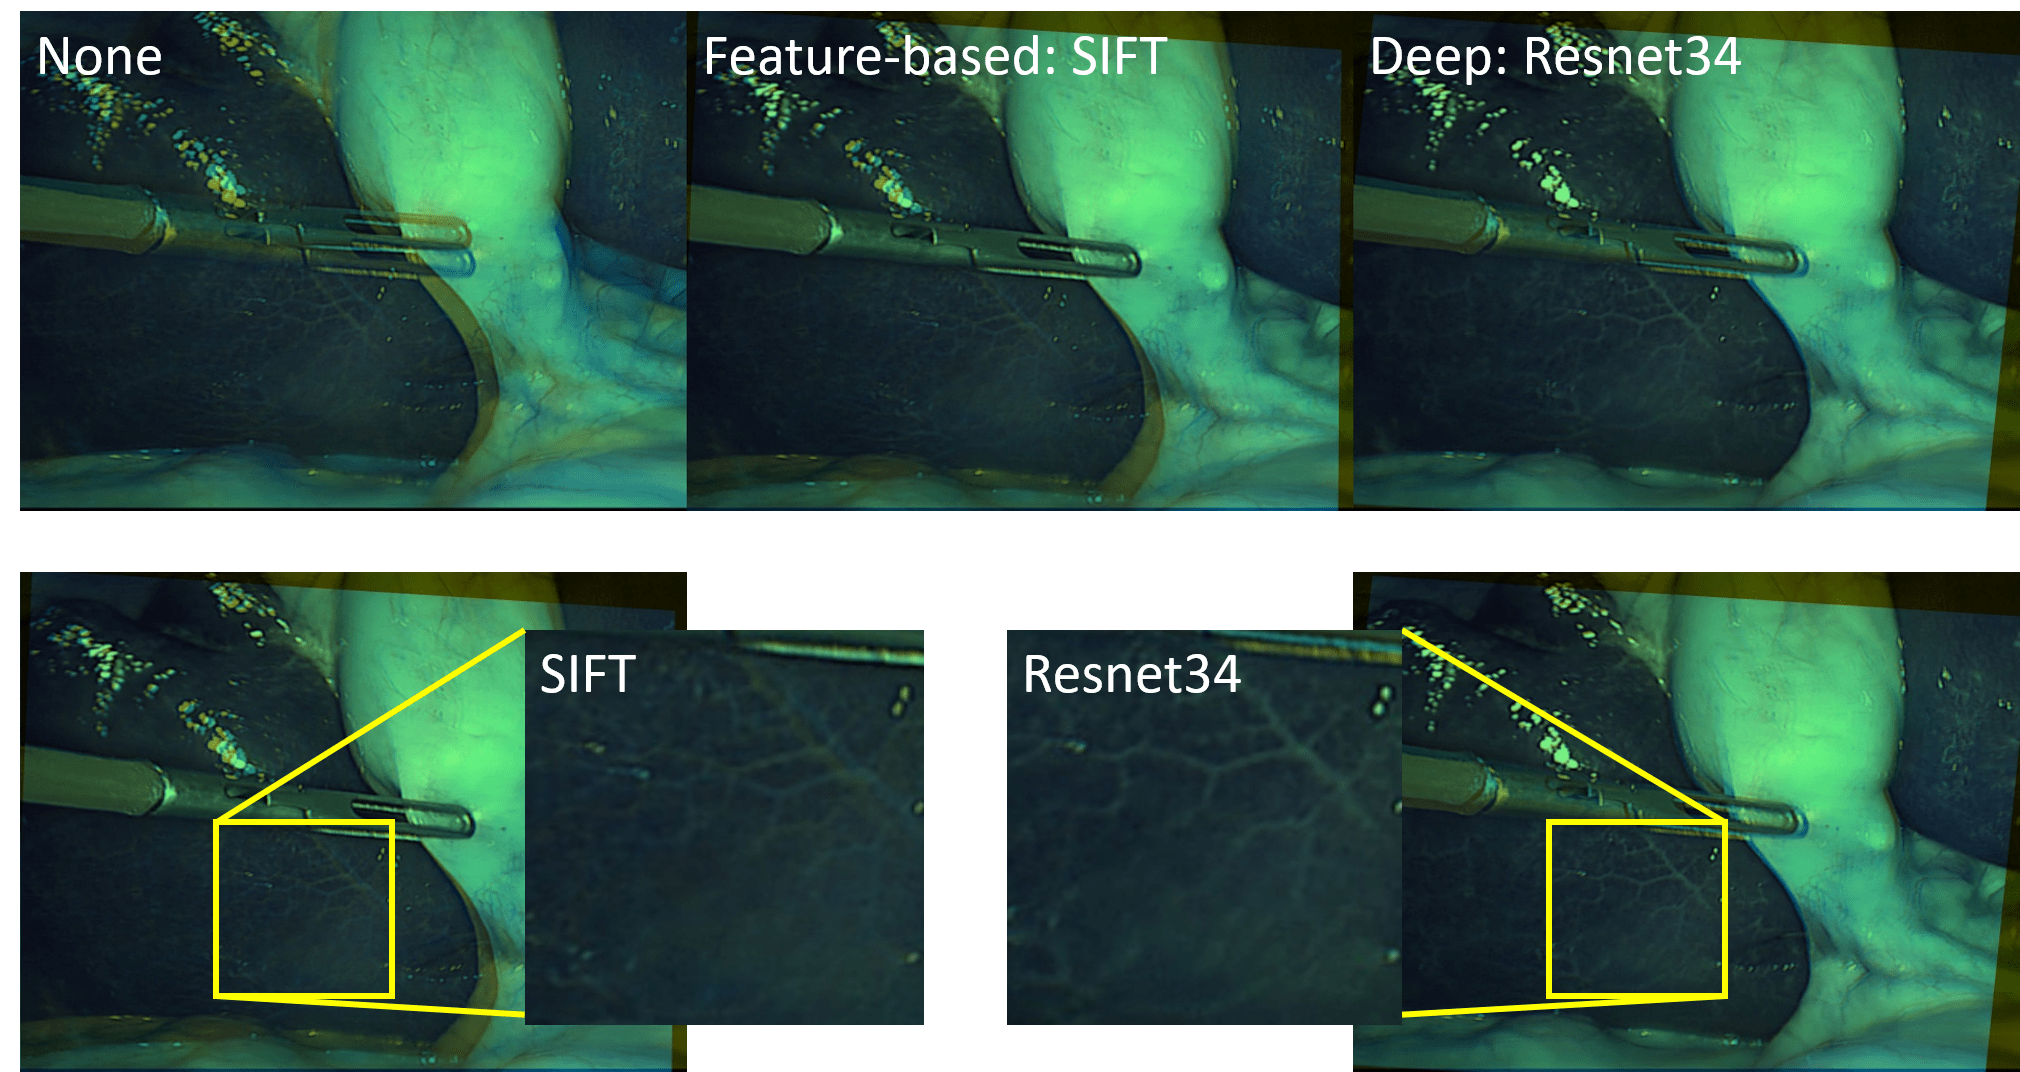
\includegraphics[width=.5\textwidth]{img/compresspng/blend_joint.png}
% 	\caption{Alpha blend of consecutive images from Cholec80 with stride $10$, corresponding to a $\Delta t$ of $0.4\,\text{s}$. Top row: The raw blend (none) shows severe camera and tool motion. The feature-based alignment breaks. The deep approach aligns both images well. Bottom row: The surgeon deforms the gallbladder while the camera is moving, the deep approach aligns the non-moving background well and ignores the deformation of the gallbladder, as can especially be seen in the zoom. Example videos of the alignment with \href{https://drive.google.com/file/d/1SpUtSVgwo_PAwAjULF-Ky_5CxRuhMYlm/view?usp=sharing}{stride 1} and \href{https://drive.google.com/file/d/17fmhSsPq290PuLXmtO-aWwo3KN4QkZA8/view?usp=sharing}{stride 10} are provided.}
% 	\label{in:fig:alpha_blend}
% \end{figure}

% Following the visual servo of \eqref{in:eq:twist}, we measure the severance of camera motion in a sequence of images by plotting the deviation of the estimated homography from the identity matrix against time, see \figref{in:fig:homography_annotation_moving_average}.

% \begin{figure}
% 	\centering
% 	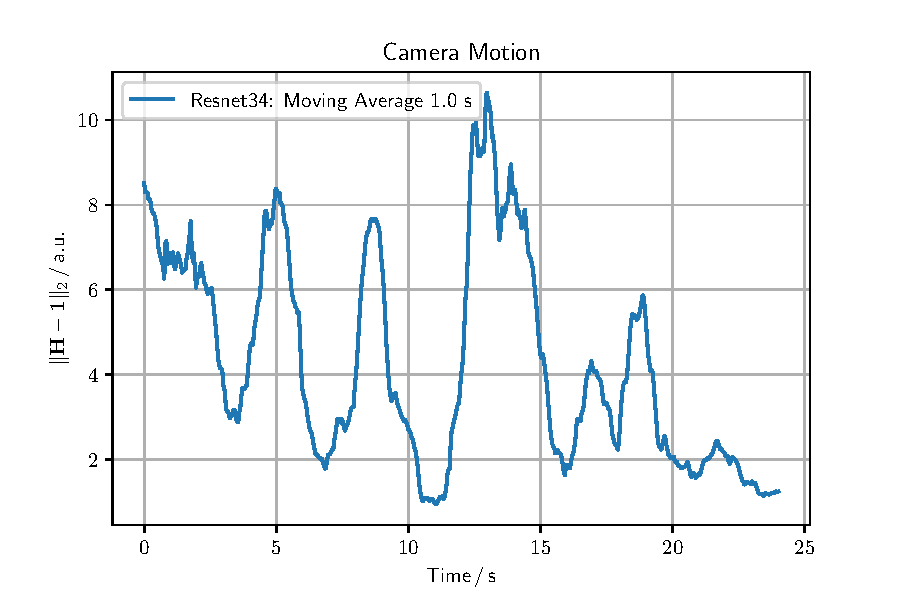
\includegraphics[width=.5\textwidth]{fig/homography_annotation_moving_average.pdf}
% 	\caption{Moving average of L2-norm of homography matrix identity deviation, similar to \eqref{in:eq:twist}. The homography was regressed in between consecutive images with stride 1 from Cholec80 using a Resnet34 backbone. The chosen metric reveals uncontinuous camera motion, as can be seen through alternating minima and maxima. This aligns well with the visual observation from video.}
% 	\label{in:fig:homography_annotation_moving_average}
% \end{figure}

% \section{OUTLOOK}
% \subsection{Conclusion}
% In this work, we are the first to combine a homography-based visual servo task with a remote center of motion objective as an enabler for deep-learning based control in robotic laparoscopic surgery. We implement said controller as a ROS package for use on any robot and demonstrate its effectiveness in \secref{in:sec:results_visual_servo}. We observe task convergence but also tip position divergence, see \figref{in:fig:visual_servo_measurements}. This is caused by the homography extraction from a distant calibration pattern, which is unresponsive to change in distance. We then generate a new dataset of da Vinci\textsuperscript{\textregistered} surgeries from which we isolate camera motion. We train multiple deep homography regression approaches and list results in \tabref{in:tab:train_results}. We find that, other than proposed in \cite{detone2016deep}\cite{nguyen2018unsupervised}\cite{zhang2019content}, a Resnet34-backboned architecture performs the best. Based on this finding and on the dataset analysis in \figref{in:fig:da_vinci_laparoscopic}, we qualitatively evaluate the deep homography regression on the unseen dataset Cholec80 in \secref{in:sec:homography_imitation_learning}. We find central views within this data with a RANSAC method, see \figref{in:fig:ransac_circle}. We observe in \figref{in:fig:alpha_blend} that this method regresses camera motion well and isolates it from object motion. We also demonstrate the superiority over traditional SIFT feature-based homography estimation. Finally, we show in \figref{in:fig:homography_annotation_moving_average} that the homography regression can be used to reveal uncontinuous camera motion in video data, which aligns well with visual observation.
% \subsection{Shortcomings and Future Work}
% Although we demonstrate future potential for the presented approach, there are still shortcomings that are yet to be addressed. The results for the visual servo were taken from simulation, the toy calibration pattern homography extraction does not yet run on the real setup. The toy homography extraction also showed diverging properties for the tip of the laparoscope in simulation, which will be addressed by replacing the type homography extraction in the future. We further note that many of the homography regression results are not yet backed by quantitative measures. This will be accounted for by creating a human-labelled ground truth data subset. To now achieve an autonomous robotic endoscope, we will extend the work starting from \figref{in:fig:homography_annotation_moving_average}, where the potential of a next best view planning was revealed from the data at hand. We will further implement a force control on the real robot for feedback to extend the pipeline into an active learning approach.

%\graphicspath{{chapter_1}}
\chapter[Marker-free Unified Eye-Hand Calibration]{Marker-free Unified Eye-Hand Calibration}
\chaptermark{Marker-free Unified Eye-Hand Calibration}
\label{chap:registration}
\minitoc

\paragraph{Disclaimer} This \chapref{chap:registration} is an \textit{in extenso} reproduction of work
%submitted
prepared
for consideration in a journal publication.
%to IEEE Transactions on Biomedical Engineering, which is currently under review.
Only \secref{c1:sec:introduction} is altered to highlight additional context within the scope of this thesis and remove redundancy with \chapref{chap:introduction}.
%\secref{in:sec:spatial_awareness}, \secref{c1:sec:robust_icp}, and \secref{in:sec:marker_free_unified_calibration} were discussed in \chapref{chap:introduction} to form a consistent picture.

\newpage

\section{Introduction}
\label{c1:sec:introduction}
Multi-robot arm systems possess an incredible potential to revolutionize the way we approach complex tasks, improving efficiency and productivity. 
By utilizing multiple arms, we can overcome the limitations of a single unit, extending the range of possible tasks that the system can perform. 
For example, suturing requires at least two arms.
There exists a wide variety of multi-robot arm applications beyond surgical robotics including 
agriculture~\cite{Xiong20}, 
civil engineering~\cite{Yasutomi23}, 
space robotics~\cite{Yan20},
packaging and assembly~\cite{Do12},
nuclear decommissioning~\cite{Mohamed07},
disaster recovery~\cite{Kamezaki16}, and
sub-sea robotics~\cite{Brantner21}.

%The da Vinci\textsuperscript{\textregistered} system by Intuitive Surgical Inc. is widely regarded as an example of a successful surgical robot system~\cite{yang2018grand, DEttorre2021} utilizing four robot arms (three for manipulation and one for imaging). However, due to its large size, incorporating the da Vinci system into the operating theater becomes arduous, restricting patient access, and making it cumbersome to remove in the event of manual intervention being required.Recently, alternative platforms have emerged that adopt a modular design where the robot arms are mounted on mobile platforms or the surgical table. 
%Examples include the 
%DLR MIRO research platform~\citep{miro}
%as well as commercial systems such as 
%the Senhance\textsuperscript{\texttrademark} Surgical System by Asensus Surgical, 
%the Hugo\textsuperscript{\texttrademark} \gls{ras} System by Medtronic, 
%the Versius\textsuperscript{\textregistered} Surgical System by \gls{cmr} Surgical, and 
%the SSI Mantra by SS Innovations.

Direct teleoperation, classified as level zero in the taxonomy proposed by Yang et al.~\cite{zhang2017automation}, is a control approach that maps signals from a surgeon-device interface onto robot motion~\cite{Niemeyer2008}, typically using position/velocity based commands.
Currently, direct teleoperation is the gold-standard for the majority of surgical robotic systems in use today. This approach guarantees that the operating surgeon is solely responsible for the robot's motion, emphasizing the need for skilled training and practice~\cite{Liu15}. Lack of training, as explained in the introductory \secref{in:sec:spatial_awareness}, may lead to severe surgical workflow interruptions. Collision models and collision avoidant control is thus desirable. A prerequisite to collision avoidant control, however, is precise localization. With the increasing automation of surgical procedures, e.g. see recent work by Saeidi et al~\cite{Saeidi2022}, the demand for localization strategies and collision models becomes even more pronounced.

% As a result, the system integration forgoes the requirement for a collision model in these multi-arm setups. 

A key requirement for future automated systems is robot base-to-base localization, i.e. each robot arm must be aware of each other arm's relative position and orientation. This is required to implement an effective collision model into the automated control system ensuring patient and the operating team's safety. In the case where multi-robot arm systems are deployed on a surgical table, base localization can be derived from \gls{cad} models, however, these measurements may not accurately reflect reality due to manufacturing inaccuracies. In the case of the increasingly popular modular systems, mentioned in \secref{in:sec:robot_surgery_platforms}, the arm setup may be different every time the theater is prepared. Furthermore, robotic systems must also undergo localization in relation to other elements present in the operating theater, including patient anatomy, lighting fixtures, imaging systems (e.g. C-arm), and so on, see \figref{in:fig:room_setup}. This motivates the need for a robot base calibration step introduced into the surgical workflow. Such a step, however, should be designed in a way that can be quickly and safely performed by non-robotics experts, i.e. the theater staff.

% The development of commercialized RGBD camera devices has been  

% Knowledge of the robot base-to-base localization is especially important in the case of the modern modular systems mentioned above.
% However, it can also be important for systems mounted on the surgical table since the measurements from \gls{cad} models may not reflect reality due to .
% need to recalibrate for modern modular systems 
% especially in the case of the modern modular systems mentioned above
% furthermore, the calibration process needs to be simplified so that it can be performed quickly by non-robotics experts
% even in case of robots being deployed on a surgical table, the \gls{cad} models may need not fully reflect reality

% Surgical robotics has become a key tool for improving patient outcomes.

% Reduced physical stress on surgeons~\citep{}.
% Reduced forces applied to trocars~\citep{} reducing damage to the incision points thus reducing recovery time, need a reference.
% Finer control/dexterity for certain tasks, e.g. suturing~\citep{}, spine 
% Furthermore, surgical robotics can enable autonomous surgery~\citep{}

% The established paradigm for surgical robots is to have a monolithic device which integrates all robot arms into a single connected device. Example systems that have adopted this design are the da Vinci\textsuperscript{\textregistered} by Intuitive Surgical, the avatera\textsuperscript{\textregistered} by avateramedical, and the hinotori\textsuperscript{\texttrademark} by Medicaroid. These are inflexible for use in the operating room, restrict patient access and are difficult to remove should the need arise for manual intervention.

% To improve flexibility, other surgical robotics platforms have adopted a new modular design paradigm where the robot arms are mounted on individual mobile platforms or the surgical table. Examples are the  DLR MIRO~\citep{miro} research platform as well as commercial systems such as the Senhance\textsuperscript{\texttrademark} Surgical System by Asensus Surgical, the Hugo\textsuperscript{\texttrademark} \gls{ras} System by Medtronic, the Versius\textsuperscript{\textregistered} Surgical System by \gls{cmr} Surgical, and the SSI Mantra by SS Innovations.

%While providing numerous benefits, the distributed paradigm brings its own issues, primarily the unknown location of the robots with respect to each other and with respect to the surgical setup. 

%- spine to robot registration
%- camera to robot registration
%- greatly simplifying setup
%- building a world map (providing a better world model)
%- robot to whatever registration for collision free path

%WHAT TASKS IN HUMAN CONTROLLED ROBOTIC SURGERY REQUIRE GOOD BASE-TO-BASE REGISTRATION?

%Autonomous surgery needs accurate base-to-base.

%This paper focuses on solving this problem



%\begin{figure}[tbh]
%\centering
%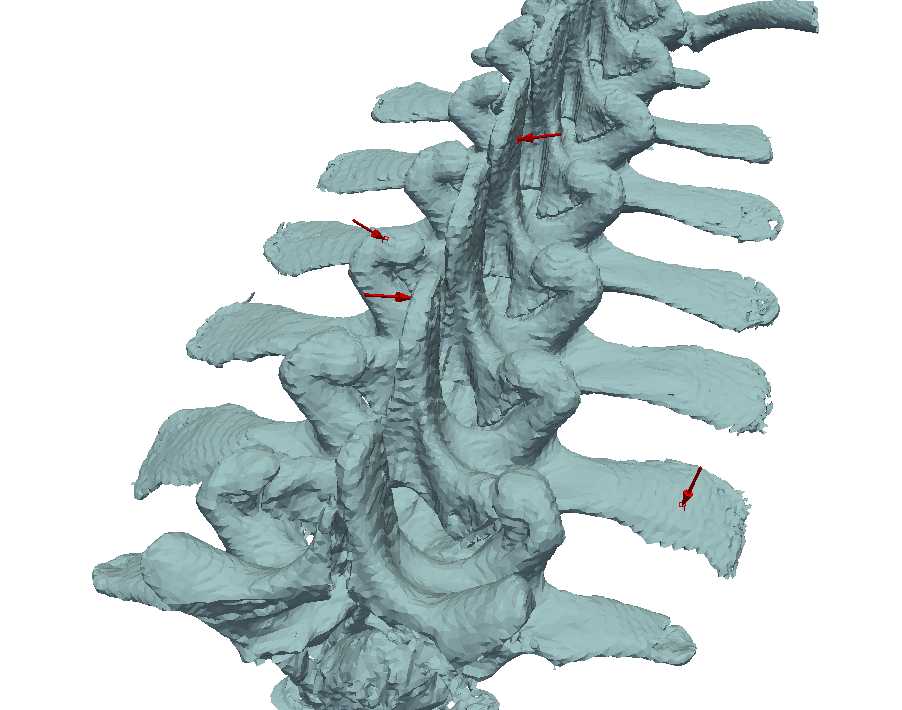
\includegraphics[width=0.45\columnwidth]{fig/preop_plan}
%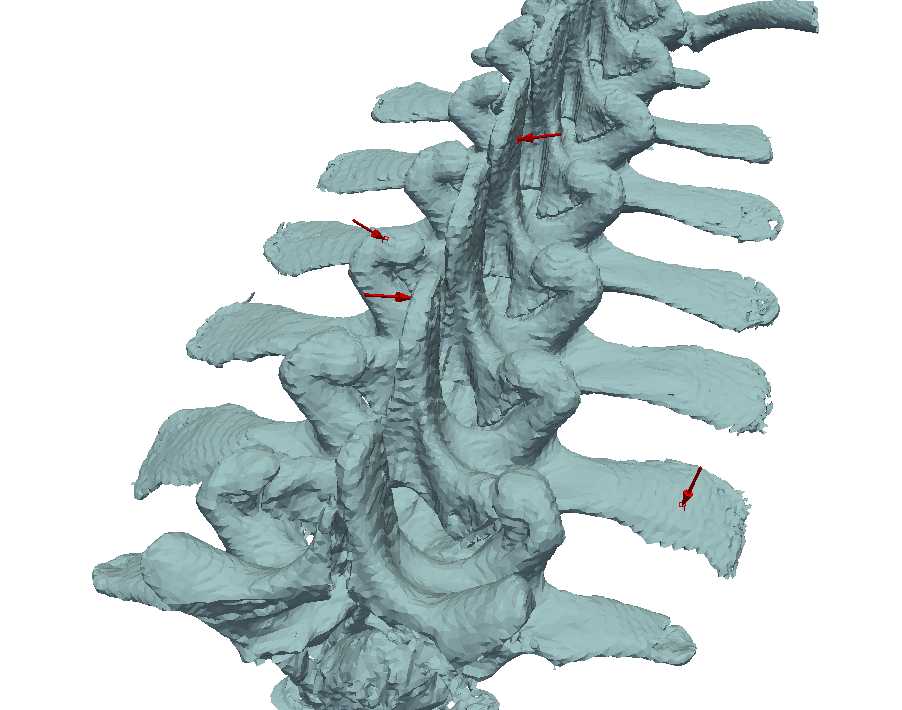
\includegraphics[width=0.45\columnwidth]{fig/preop_plan}
%\caption{The preoperative plan (left) and the corresponding surgical site (right). The arrows on the left-hand image show the planned imaging targets that will be executed by the robot.} 
%\label{c1:fig:preop_plan}
%\end{figure}



\subsection{Contributions}
\begin{figure}[tb]
    \centering
    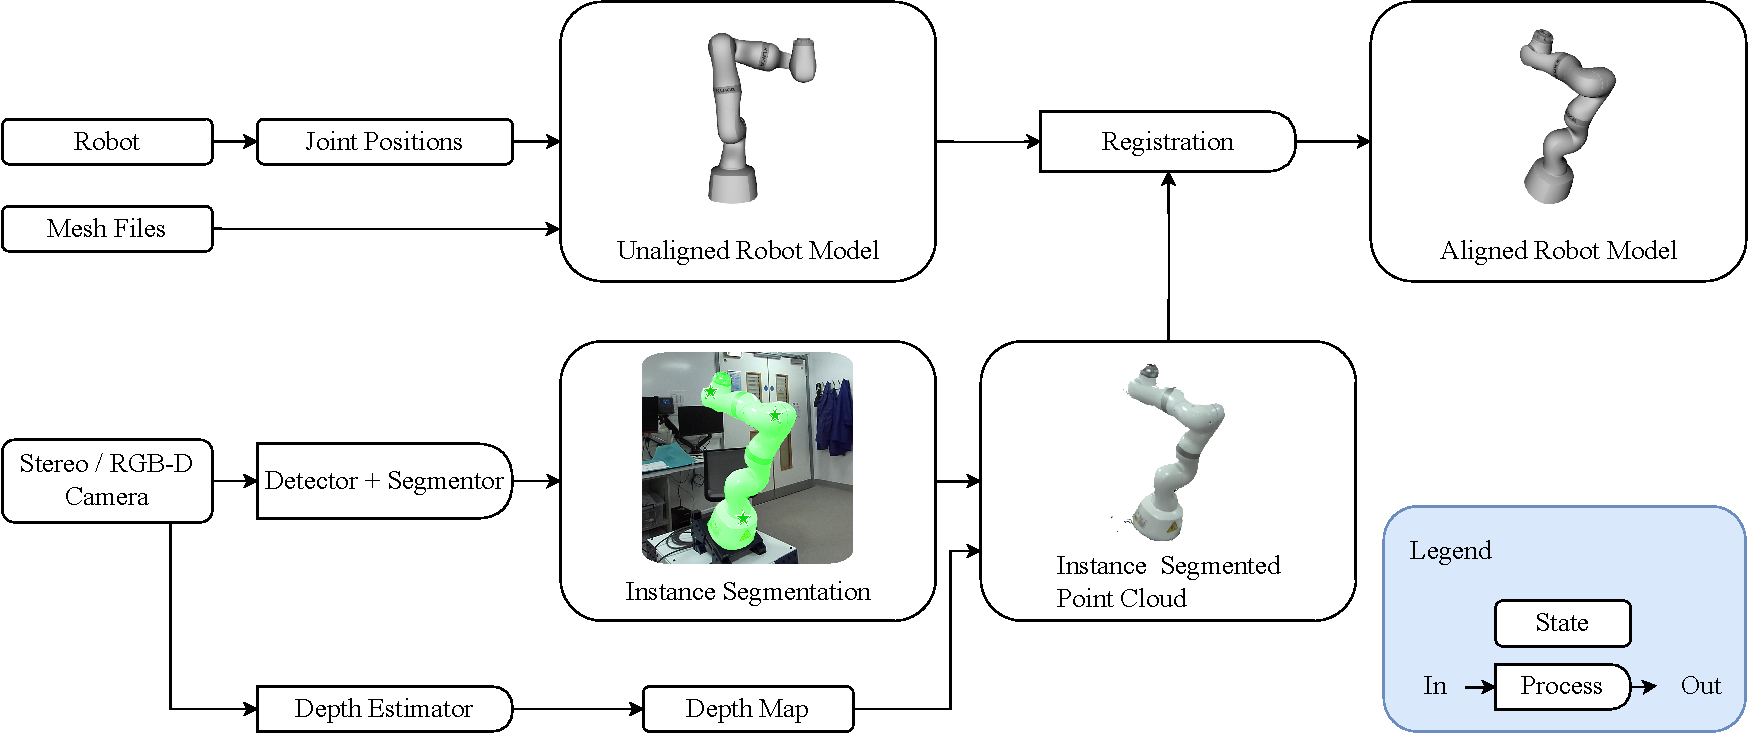
\includegraphics[width=\textwidth]{chapter_1/fig/approach_refined.pdf}
    \caption{Proposed registration procedure. The pipeline takes joint positions and corresponding stereo or RGB-D images as input and yields eye-to-hand transformations. Upper half: Joint positions from the robot(s) are used to transform the link mesh files into an unaligned robot model. Lower half: Stereo (or RGB-D) images are fed through a depth estimator to obtain a depth map. A monocular image is taken from the stereo image and is used to detect and instance segment the robot. The depth map and instance segmentation are fused to obtain an instance-segmented point cloud. The instance-segmented point cloud is registered to the unaligned robot model to obtain a robot model that is aligned with the observed image. The transform from unaligned to aligned robot model describes the robot to camera homogeneous transform $\homogeneous{C}{B}$. Refers to \secref{c1:sec:proposed_calibration_procedure}.}
    \label{c1:fig:calibration_pipeline}
\end{figure}
In this work we make the following contributions:
\begin{itemize}
    \item A unified approach for eye-in-hand and eye-to-hand calibration of multiple surgical robots with no need for any calibration targets since the robot itself is used instead. Our proposed method uses a novel robust \gls{icp} formulation of a point-to-plane objective on a Lie algebra. Only RGB-D images, the robots' joint positions, and their respective mesh files or \gls{cad} models are used.
    \item We conduct several benchmarks comparing our methods against classical approaches. Our method ensures safety and, based on the comparisons, demonstrates faster execution and better outcomes when compared to other options.
    \item Hardware realization of the approach on a dual robot arm system. Furthermore, we showcase a human-robot collaboration through admittance control with arm-arm collision avoidance. The collision model for the two robots relies on the measurements generated by our proposed method.
    %The two robots are controlled in a collision avoidant manner.
    % Upon acceptance of this manuscript, our intention is to make the code-base publicly available as an open-source contribution. This will encompass both the proposed method itself and the \gls{phri} controller, that includes integrated collision avoidance functionality.
    \item We conduct an in-vivo experiment in a clinically relevant dual-arm setup for spine surgery.
\end{itemize}

% We present a method of providing base-to-base registration for two or more surgical robots using a stereo or RGB-D camera. The method uses the current joint states of each arm to configure the arm's mesh, which is then fitted to the point cloud using the Iterative Closest Point (ICP) method.
% We compare our results to handshaking and show our results to be comparable while taking much less time to perform.


% It provides a unified approach to eye-in-hand and eye-to-hand calibration and does not require any calibration targets, since it uses the robot as calibration target itself.

\section{Related Work}
\subsection{Eye-in-hand Calibration}
Prior work on the eye-in-hand problem~\cite{Horaud95, Strobl06} require the user to fabricate a marker (e.g. checkerboard or AprilTag~\cite{Olson11}) with known geometry making it easy to extract a pose from images. In our work, we do not require the user to create such a marker.
Instead, we make use of the mesh files or \gls{cad} models provided by the manufacturer.

\subsection{Marker-free Registration}
Marker-free eye-to-hand calibration is an active research field with new developments being lead by differentiable rendering frameworks, such as PyTorch3D~\cite{ravi2020pytorch3d} and Kaolin~\cite{KaolinLibrary}. Consequentially, some works utilize these frameworks to optimize for camera poses such that mesh renders match image segmentations~\cite{Chen:RAL:2023}. Further work proposes a fully self-supervised procedure that learns both, to segment and to estimate the eye-to-hand transformation~\cite{lu2023markerless}. These works require tailoring to dedicated robot models and depend on fully-blown differentiable rendering pipelines, which makes them difficult to use in practise.
~\citet{labbe2021single} use classical non-differentiable rendering, where the authors also predict joint states on top of the eye-to-hand registration. This work also requires training to dedicated systems. Simpler approaches suggest to predict robot joint positions and extract eye-to-hand registrations through solving a \gls{pnp} problem~\cite{lee2020camera}. In this work, we suggest a conceptually much simpler approach that works for any robot, but uses RGB-D images, and, as some of the other methods, robot joint states. Closest to our work comes~\cite{point_cloud_based_robot_cell_calib}, where the authors also perform point cloud registration. Their method, however, only registers a single configuration and performs complex clustering of the observed point cloud. The only marker-free work on a surgical system is presented in~\cite{hand_eye_calibration_robotic_assisted}, where the authors utilize the surgical tools as calibration target. Whilst being quite appealing, this method does not allows for external collision avoidance nor hybrid setups.

% TODO:~\cite{point_cloud_based_robot_cell_calib} highly complex point cloud pre-processing 

% TODO:~\cite{hand_eye_calibration_robotic_assisted}: requires inserted tools, uses tools as calibration target, does not allows for external tracking collision avoidance etc... 

\section{Problem Formulation}
\begin{figure}[tb]
    \centering
    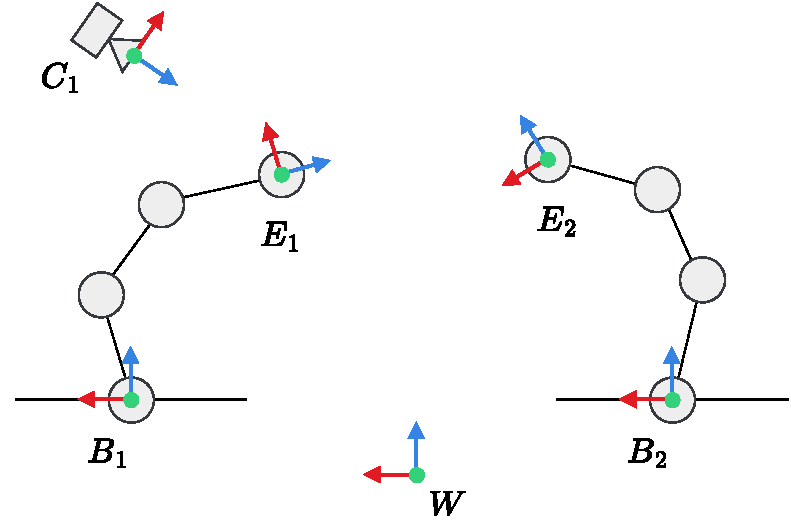
\includegraphics[width=0.8\textwidth]{chapter_1/fig/eye_in_to_hand.pdf}
    \caption{
    Schematic overview of the key coordinate frames of interest for this work. Base-to-base calibration is achieved via two eye-to-hand calibrations. Whilst we show a dual arm system, it is easy to extend the methods discussed in this paper to multiple robots.
    }
    \label{c1:fig:base2base}
\end{figure}
In this section, we formally present the two problems that our research addresses. The key coordinate frames are illustrated in the schematic diagrams shown in \figref{in:fig:eye_to_hand}, and \figref{in:fig:eye_in_hand}, for the eye-to- and eye-in-hand scenarios, respectively. \figref{c1:fig:base2base} adds additional nomenclature for the base-to-base via dual eye-to-hand calibration. The following subsection introduces the notation employed in the entirety of this paper and also states some important assumptions we make to facilitate our approach. 
Subsequently, we outline our problems in the remaining subsections.

\subsection{Notation and Assumptions}
In general, we use letters (e.g. $a, \alpha$) to denote scalars, bold letters (e.g. $\mathbf{a},\boldsymbol{\alpha}$) to denote vectors, 
capital bold letters (e.g. $\mathbf{A}, \mathbf{\Gamma}$) to denote matrices, and 
calligraphy and blackboard formats (e.g. $\mathcal{A}, \mathbb{B}$) to denote sets and spaces.

\paragraph{Coordinate Frame Transformations} A homogeneous transformation matrix, denoted $\homogeneous{B}{A}\in\mathbb{R}^{4 \times 4}$, represents the pose of frame $A$ with respect to $B$ (i.e. $B$, in this case, is the base frame).
The matrix $\homogeneous{B}{A}$ can be expressed as
\begin{equation}
\homogeneous{B}{A} = 
    \begin{bmatrix}
     \mathbf{R}\big({}^{B}\mathbf{q}_{_A}\big) & {}^{B}\mathbf{p}_{_A} \\
     \mathbf{0}^{1\times3} & 1
    \end{bmatrix}
    \label{c1:eq:ht}
\end{equation}

where ${}^{B}\mathbf{p}_{_A}\in\mathbb{R}^3$ is a column vector representing the position, $\mathbf{R}:\mathbb{R}^4\rightarrow\mathbb{R}^{3\times 3}$ is function that converts the unit-quaternion ${}^{B}\mathbf{q}_{_A}\in\mathbb{R}^4$ to a rotation matrix, and $0_3$ is the three element row vector containing only zeros.
With reference to the schematic of a robot arm in \figref{in:fig:eye_in_hand}, the camera frame $C$ is expressed in the end-effector frame $E$ by $\homogeneous{E}{C}$, and $E$ is expressed in the robot base frame $R$ by $\homogeneous{R}{E}$. 
%and
%$R$ is expressed in the world frame $W$ by $\homogeneous{R}{R}$.
%Therefore, the camera frame $C$ expressed in the world frame $W$ is found using
%\begin{equation}
%    \homogeneous{R}{C} = \homogeneous{R}{R} \homogeneous{R}{E} \homogeneous{E}{C}.
%\end{equation}

\paragraph{Forward Kinematics} For an $N$-\gls{dof} robot manipulator, the joint positions are denoted $\mathbf{x}\in\mathbb{R}^N$. In this work, we assume that the end-effector frame $E$ expressed in the robot base frame $R$, i.e. $\homogeneous{R}{E}$, can be computed accurately using forward kinematics. We denote the relationship between the joint positions and link poses, including the end-effector, by
\begin{equation}
    \begin{pmatrix}
         {}^{R}\mathbf{p}_{_L}\\
         {}^{R}\mathbf{q}_{_L}
    \end{pmatrix}
    = \phi(\mathbf{x}),
    \label{c1:eq:fk}
\end{equation}

where $\phi: \mathbb{R}^N\rightarrow\mathbb{R}^{7}$ represents the forward kinematics function. Given a geometric description of the robot's joints and links (typically in the common URDF format), the forward kinematics $\phi(\cdot)$ is easily derived.

\paragraph{Modality Prerequisites} Regarding the camera, that is either placed in the environment, as in \figref{c1:fig:base2base}, or mounted at the robot end-effector, as in \figref{in:fig:eye_in_hand}, we assume stereo or RGB-D. Finally, we assume access to the mesh files or \gls{cad} models for each of the robot arms.

%\subsection{Robot Base-to-base Calibration}

%In this subsection, we primarily describe the problem associated with \figref{c1:fig:base2base}. As discussed above, several robots could be positioned at once in the operating theater. To enable automated approaches, these robot arms must be aware of the other's position and orientation. With reference to \figref{c1:fig:base2base}, the transforms $\homogeneous{{E_i}}{{R_i}}$ are assumed known for each $i\in[1, 2]$. The goal of this work is to utilize information from the camera located at frame $C$, and with the mesh files or \gls{cad} models to compute estimates for the transforms $\homogeneous{C}{{B_1}}$ and $\homogeneous{C}{{B_2}}$. Given estimates for these frames, we can thus compute one robot pose with respect to the other. This can be expressed by

%\begin{equation}
    %\homogeneous{{B_1}}{{B_2}} = \homogeneous{{B_1}}{C} \homogeneous{C}{{B_2}} = \homogeneous{{B_1}}{C} (\homogeneous{{B_2}}{C})^{-1}
%\end{equation}
%where superscript -1 denotes the matrix inverse. 

%\subsection{Eye-in-hand calibration}

%In this subsection we primarily describe the problem associated with \figref{in:fig:eye_in_hand}.
%Sensors, such as cameras, are often mounted at the robot end-effector in order to perform imaging tasks.
%Often, the transform between the camera frame $C$ and the robot end-effector $E$ is not known.
%Often \gls{cad} models are available for the mount which attaches the camera to the end-effector.
%However, the precise location of the camera imaging sensor is not known accurately, i.e. the camera extrinsic parameters.

%Estimating the unknown static transformation frame $\homogeneous{E}{C}$ is a problem we address in this work as part of our unified approach.
%This is the so-called \textit{eye-in-hand}, or also known as \textit{hand-eye}, calibration problem~\cite{Horaud95}.
%An additional consideration regarding this problem, is that the static transform $\Theta^W_R$ is often also unknown.
%The majority of previous approaches in the literature attempt to solve the ill-posed problem $\Theta^W_C \Theta^R_W = \Theta^E_C \Theta^R_E$.
%Typically, a marker (e.g. checkerboard) of known geometry is affixed to the world frame $W$ that can be estimated and provide an estimate for the transformation frame $\Theta^C_W$ (assuming properly calibrated camera intrinsic parameters).
%As mentioned as an assumption above, the forward kinematics can provide an accurate estimate for the transformation $\Theta^R_E$.
%Multiple images from the camera at various joint positions are taken, and thus recording multiple measurements for $\Theta^C_W$ and $\Theta^R_E$.
%In order to simplify notation, let us denote the unknowns by $X=\Theta^R_W$ and $Y=\Theta^E_C$ and the known values $A_i=\Theta^W_C = (\Theta^C_W)^{-1}$ and $B_i=\Theta^R_E$ (the subscript $i$ refers to the fact that we take multiple measurements), thus the eye-in-hand problem can be re-written as $A_i X = Y B_i$.

%The standard formulation of the eye-in-hand %calibration problem is expressed by
%\begin{equation}
%\label{c1:eq:eyeinhand}
%    \widehat{X}, \widehat{Y} = \underset{X, Y\in\mathbb{R}^{4\times 4}}{\text{arg}\min}~\sum_i \| A_i X - Y B_i\|^2
%\end{equation}
%where $\widehat{X}, \widehat{Y}$ are the solution to the least squares problem and represent estimated homogeneous transformation matrices.
%In our work, we remove the need for a marker affixed in the environment.
%Instead, we make use of the mesh files or \gls{cad} model for the robot arm.
%This requires a reformulation of Equation~\ref{c1:eq:eyeinhand}, which we discuss in later sections.

\section{Materials and Methods}
\label{c1:sec:materials_and_methods}
\begin{figure}[htb]
    \centering
    \includegraphics[width=\textwidth]{chapter_1/fig/hydra_registration.pdf}
    \caption{Detailed point cloud generation and acquisition including pre-processing steps for the proposed robust point-to-plane \gls{icp}. Refers to \secref{c1:sec:robust_icp}.}
    \label{c1:fig:hydra_registration}
\end{figure}

This section introduces a baseline base-to-base calibration procedure via handshake in \secref{c1:sec:handshake_calibration}. For the eye-in/to-hand scenarios, baselines as introduced in \secref{in:sec:eye_in_to_hand_calibration} are utilized. The baseline calibration procedures are considered the reference for the proposed calibration method. The proposed calibration method is explained outlined in \secref{c1:sec:proposed_calibration_procedure} and an overview is given in \figref{c1:fig:calibration_pipeline} and \figref{c1:fig:hydra_registration}. Instantiations thereof, through a simple \gls{icp}, and our novel robust point-to-plane \gls{icp}, are detailed in \secref{c1:sec:simple_icp_registration} and \secref{c1:sec:robust_icp}, respectively.

In the following sections, homogeneous transforms, from the coordinate frame $A$ to $B$, are denoted through Equation~\ref{c1:eq:ht}
% \begin{equation}
    % \homogeneous{{B}}{A}=\begin{bmatrix} {}^B\mathbf{R}_A & {}^B\textbf{t}_A \\ \mathbf{0} & 1 \end{bmatrix}
% \end{equation}
% where the rotation matrix $^B\mathbf{R}_A$ and the translation vector $^B\textbf{t}_A$.
The world coordinate frame is indicated by $W$. The world coordinate frame $W$ is considered to coincide with the robot base coordinate frame $B$. $W$ and B may thus be used interchangeably. The camera coordinate frame is highlighted through $C$. Furthermore, $A$ indicates the coordinate frame of an ArUco marker.

\subsection{Base-to-base Calibration Baseline}
\label{c1:sec:handshake_calibration}
For the handshake calibration procedure, the two robots are rigidly linked to one another at their end-effectors via a calibration fixture of estimated transform $\homogeneous{{E_1}}{{E_2}}$, see \figref{c1:fig:handshake}. The robots are then moved in admittance control mode and $L$ base-to-end-effector samples are collected for both robots, i.e. $\homogeneous{{B_1}}{{E_1}}^l$ and $\homogeneous{{E_2}}{{B_2}}^l$. Since the system forms a closed kinematic chain, the base-to-base transform $\homogeneous{{B_2}}{{B_1}}$ can then be obtained by minimizing:
%
\begin{equation}
    \label{c1:eq:handsake}
    \min_{\homogeneous{{E_1}}{{E_2}}, \homogeneous{{B_2}}{{B_1}}} \sum_{l=0}^{L-1}\,\homogeneous{{B_1}}{{E_1}}^l\,\homogeneous{{E_1}}{{E_2}}\,\homogeneous{{E_2}}{{B_2}}^l\,\homogeneous{{B_2}}{{B_1}} - \mathbf{I}^{4\times4},
\end{equation}
%
where $\mathbf{I}^{4\times4}$ is the $4\times4$ identity matrix. Therein, $\homogeneous{{E_1}}{{E_2}}$ is part of the optimization to correct for manufacturing errors.

% Classically, eye-in-hand calibration is conducted by collecting end-effector to base $\homogeneous{B}{E}$ and camera to ArUco marker transformations $\homogeneous{A}{C}$~\citep{eye_in_hand}. The correspondences are re-arranged into an equation of the form $\mathbf{A}\mathbf{X}=\mathbf{X}\mathbf{B}$, with $\mathbf{A}$ containing multiple $\homogeneous{{E_j}}{{E_i}}$ and $\mathbf{B}$ containing multiple $\homogeneous{{C_j}}{{C_i}}$. A 2-step regression is applied to solve for $\mathbf{X}=\homogeneous{{B_2}}{{B_1}}$.

\subsection{Proposed Registration Procedure}
\label{c1:sec:proposed_calibration_procedure}
A high-level overview of the proposed method is shown in \figref{c1:fig:calibration_pipeline}. The method provides an efficient way to find the homogeneous transformation from the robot base frame to the camera frame $\homogeneous{C}{B}$. It aligns an unaligned robot model to an observed instance-segmented point cloud through registration. Importantly, the instance-segmented point cloud and unaligned robot model must be synchronized. The unaligned robot model and the instance segmentation are detailed in \secref{c1:sec:unaligned_robot_model_and_instance_segmented_point_cloud}. 

For the registration step in \figref{c1:fig:calibration_pipeline}, we investigate a simple \gls{icp} algorithm and derive a robust point-to-plane \gls{icp} on a Lie algebra. The simple \gls{icp} variant of the registration procedure is explained in \secref{c1:sec:simple_icp_registration} and the robust point-to-plane \gls{icp} variant in \secref{c1:sec:robust_icp}. A single snapshot is sufficient to find the transformation, which differentiates it from classical calibration procedures described in \secref{c1:sec:handshake_calibration}. In the case of a robot-mounted camera, i.e. eye-in-hand calibration illustrated in \figref{c1:fig:eye_in_hand}, the calibration can be used to determine the transformation from robot end-effector to camera $\homogeneous{C}{E}$. In the case of an externally mounted camera, i.e. eye-to-hand calibration illustrated in \figref{c1:fig:eye_to_hand}, the calibration can be used to determine the robot base-to-base transformation $\homogeneous{{B_2}}{{B_1}}$ through $\homogeneous{{B_2}}{{B_1}} = \homogeneous{C}{{B_2}}^{-1}\,\homogeneous{C}{{B_1}}$.

\subsubsection{Unaligned Robot Model and Instance-segmented Point Cloud}
\label{c1:sec:unaligned_robot_model_and_instance_segmented_point_cloud}
\paragraph{Unaligned Robot Model}
\label{c1:sec:unaligned_robot_model}
To obtain an unaligned robot model, the proposed registration procedure takes as input measured joint positions $\mathbf{x}_t$ and link mesh files $\mathcal{M} = \{M_i\}$. Only the mesh vertices $\mathcal{V} = \{\mathbf{V}_i\}$ are extracted from the meshes and everything else, e.g. color, is discarded. All mesh vertices $V_i$ are then transformed through $\homogeneous{{L_i}}{R}$, where, given the joint positions, $\homogeneous{{L_i}}{R}$ is obtained via forward kinematics $\phi(\mathbf{x}_t)$, see Equation~\ref{c1:eq:fk}. From the transformed mesh vertices $\mathcal{V}$, we sample a total of $N$ points. Since small meshes in \gls{cad} files often contain disproportionately many vertices, we normalize the sampled vertices per link by volume. Therefore, we estimate the volume that each link occupies through its respective bounding box volume $b(\mathbf{{V}):\mathbb{R}}^M \rightarrow \mathbb{R}$. We then sample $n_i$ points per link vertices $\mathbf{V}_i$ via a Poisson-disk sampling strategy, where
\begin{equation}
    n_i = N\frac{b(\mathbf{V}_i)}{\sum_j b(\mathbf{V}_j)}.
\end{equation}
This sampling strategy guarantees somewhat equally distributed points in space, although future version might only want to perform Poisson-disk sampling over the entire robot.

%Mesh files usually contain interior points, which cannot be observed by the stereo or RGB-D camera. Interior points would indeed confuse the registration discussed in \secref{c1:sec:simple_icp_registration}. To obtain only points that lie on the alpha shape of the mesh, sometimes referred to as the concave hull, we utilize a simple sampling strategy. We specify a bounding box that has the meshes' center of mass at the center. We then uniformly sample N points on the bounding box and for each find the closest point on the mesh. These steps result in in the unaligned robot model, that is the robot model's base frame coincides with the camera coordinate frame.

\paragraph{Instance-segmented Point Cloud}
\label{c1:sec:instance_segmented_point_cloud}
The instance-segmented point cloud is generated by fusing an instance segmentation $\mathbf{S}_t$ with a depth map $\mathbf{D}_t$ as shown in \figref{c1:fig:calibration_pipeline}. For the instance segmentation, we combine a detector with a segmentor. In this work, a human-in-the-loop acts as the detector by selecting a few points $\mathcal{F}_t$ on the robot in the image. We then deploy the pre-trained \gls{sam}~\cite{Kirillov:iccv:2023} and prompt it with the detection points $\mathcal{F}_t$. We thus achieve an instance segmentation $\mathbf{S}_t$ of the image $\mathbf{I}_t$ with zero-shot training. The depth map $\mathbf{D}_t$ can either be obtained via a stereo camera or an RGB-D camera by processing it with a depth estimator. In this work, we utilize Stereolab's Neural Depth perception as the depth estimator. Since both, the image segmentation $\mathbf{S}_t$ and the depth map $\mathbf{D}_t$, are observed from the same camera coordinate system, one may simply keep depth values where there is a segmentation and discard all others, i.e. compute the Hadamard product. This procedure then provides the instance segmented point cloud.


% The following sections will explain an \gls{icp} registration on Lie-algebra for said purpose in \secref{c1:sec:robust_icp}. Following that, image-based registration refinements, given a segmentation mask without the need for differentiable rendering are explained in \secref{in:sec:registration_of_3d_point_cloud}.

\subsection{Simple ICP Registration}
\label{c1:sec:simple_icp_registration}
In the case of the simple \gls{icp} we perform single instance registration. The goal is to align the unaligned robot model (as detailled in \secref{c1:sec:unaligned_robot_model}), with the instance-segmented point cloud (as detailled in \secref{c1:sec:instance_segmented_point_cloud}), through finding the transform $\homogeneous{C}{B}$. First, the unaligned robot model $\mathcal{V}_\tau$ is generated (as detailled in \secref{c1:sec:unaligned_robot_model}). Next, robot instances are detected and segmented, which results in the instance-segmented point cloud $\mathbf{P}_\tau$. We then compute the instance-segmented point cloud's center of mass for an initial guess of the transform $\homogeneous{{C}}{B,\text{init}}$. Finally, we run an \gls{icp}~\cite{simple_icp} algorithm between vertices $\mathcal{V}_\tau$ and point cloud $\mathbf{P}_\tau$, see Equation~\ref{c1:eq:icp}. In contrast to~\cite{simple_icp}, we only consider vertices from $\mathcal{V}_\tau$ whose surface normals point towards the camera. That is, they should be visible to the camera.

\begin{equation}
    \label{c1:eq:icp}
    \text{ICP} = \argmin_{\homogeneous{C}{B}} || \homogeneous{C}{B}(\mathcal{V}_\tau) - \mathbf{P}_\tau||_2
\end{equation}

\subsection{Robust Point-to-plane ICP Registration: A Lie Algebra Formulation}
% \subsubsection{Point-to-plane ICP: A Lie Algebra Formulation}
\label{c1:sec:robust_icp}
\begin{algorithm}
\caption{A recap of the robust Lie group formulation of the point-to-plane ICP.}\label{c1:alg:liep2plan}
\begin{algorithmic}
\State Let $\{p\}$ be points to match (the observations). We omit the indices for simplicity here
\State Let $\{q,n\}$ be points with associated normals (the model)
\State Let $t \gets 0$ be a counter for the outer iterations
\State Let $\Theta_0 = \{R_0,T_0\}$ be an initial estimate of the transformation parameters
\While{ICP not converged}
  \State Compute the transformed points $\Theta_t p$
  \State Perform an approximate nearest neighbour search to match $\Theta_t p$ and $q$ points
  \State Discard point pairs associated with distances that are definitely outliers
  \State We now use $i$ indices to indicated matching points
  \State Compute the residuals: $b_i \gets \tilde{n}_i^T (\tilde{q}_i - R_t \tilde{p}_i - T_t)$
  \State \Comment{Previous computation of $\Theta_t p$ should of course be re-used here}
  \State Compute the robust standard deviation: $\sigma \gets \MAD(\{b_i\})/0.6745$
  \State \Comment{Done once to avoid recomputing it in the inner iterations}
  \State Let $\tau \gets 0$ be a counter for the inner iterations
  \State Let $\Theta_{t,0} \gets \Theta_{t}$ be the current estimate of the transformation
  \While{Gauss-Newton not converged}
    \If{$\tau \neq 0$}
      \State Compute the residuals: $b_i \gets \tilde{n}_i^T (\tilde{q}_i - R_{t,\tau} \tilde{p}_i - T_{t,\tau})$
    \EndIf
    \State Compute the robust weights: $\omega_i \gets \omega_{1.345\sigma}(b_i)$
    \State Compute the linear coefficients: $a_i \gets [-\tilde{n}_i^T R_{t,\tau} {{\tilde{p}}_{i\times}}, \tilde{n}_i^T R_{t,\tau}]$
    \State Solve the weighted normal equation:
    \State \quad $\delta\Theta \gets \texttt{chol\_solve}(A^T W A, A^T W B)$
    \State Update the transformation: $\Theta_{t,\tau+1} \gets \Theta_{t,\tau} \cdot \exp(\delta\Theta)$
    \State $\tau \gets \tau+1$
  \EndWhile
  \State Let $\Theta_{t+1} \gets \Theta_{t,\tau}$
  \State $t \gets t+1$
\EndWhile
%\Require $n \geq 0$
%\Ensure $y = x^n$
%\State $y \gets 1$
%\State $X \gets x$
%\State $N \gets n$
%\While{not converged}
%\If{$N$ is even}
%    \State $X \gets X \times X$
%    \State $N \gets \frac{N}{2}$  \Comment{This is a comment}
%\ElsIf{$N$ is odd}
%    \State $y \gets y \times X$
%    \State $N \gets N - 1$
%\EndIf
%\EndWhile
\end{algorithmic}
\end{algorithm}
To guarantee robust convergence of the noisy point cloud to the robot mesh, we further propose a robust point-to-plane \gls{icp} formulation. We capture multiple configurations of the robot. An overview of the method is provided in \figref{c1:fig:hydra_registration}. Deviating from the simple \gls{icp}, \secref{c1:sec:simple_icp_registration}, we dilate the instance segmentations $\mathbf{S}_t$ and only keep the boundary regions. Consequentially, we also only keep the boundary regions of the instance segmented point clouds $\mathcal{P} = \{\mathbf{P}_t\}$. Similarly to the simple \gls{icp}, we compute the centroids for the instance segmented point clouds $\{\mathbf{P}_t\}$ as well as for each robot model $\{\mathcal{V}_t\}$. We then use the Kabsch algorithm to find an initial estimate for the camera to base homogeneous transformation through centroid alignment. Given the initial alignment, we then perform a robust point-to-plane registration on a Lie algebra, as further detailed below.
%We follow the derivation of \chapref{chap:introduction}, \secref{c1:sec:robust_icp}. A summary for which is provided in \algoref{c1:alg:liep2plan}.

% Tom's notes
% \subsubsection{Point-to-plane ICP: A Lie Algebra Formulation}
% \label{in:sec:p2plane}

\paragraph{Basic Formulation}
We first introduce the problem solved by the point-to-plane \gls{icp} algorithm~\cite{Rusinkiewicz:IC3DIM:2001}.
Let $\mathbf{p}_i$ and $\mathbf{q}_i$ be corresponding 3D points in homogeneous coordinates. Let $\mathbf{n}_i$ be a normal vector associated with $\mathbf{q}_i$. We search a rigid body transformation $\mathbf{\Theta}$ in $SE(3)$ that minimizes:
\begin{equation}
\sum_i ||\mathbf{n}_i^T \cdot (\mathbf{\Theta} \cdot \mathbf{p}_i - \mathbf{q}_i)||^2 = \sum_i (\mathbf{n}_i^T \cdot \mathbf{\Theta} \cdot \mathbf{p}_i - \mathbf{n}_i^T \cdot \mathbf{q}_i)^2
\end{equation}

\paragraph{Iterative Optimization on the $SE(3)$ Lie Group}
Let $\mathbf{\Theta}_0$ be the current estimate. In a Lie group iterative optimization approach~\cite{Mahony:JGO:2002,Vercauteren:IPMI:2007}, we seek a perturbation $\Delta\mathbf{\Theta} \in \mathfrak{se}(3)$ composed with
$\mathbf{\Theta}_0$: $\mathbf{\Theta}_1 = \mathbf{\Theta}_0 \cdot \exp(\Delta\mathbf{\Theta})$. We now seek to minimize:
\begin{equation}
\sum_i (\mathbf{n}_i^T \cdot \mathbf{\Theta}_0 \cdot \exp(\Delta\mathbf{\Theta}) \cdot \mathbf{p}_i - \mathbf{n}_i^T \cdot \mathbf{q}_i)^2
\end{equation}

\paragraph{Mathematical Preliminaries}
For convenience, we take advantage of the relationship between the 3D cross product, the Lie bracket on SO(3), and the skew-symmetric matrix operator.
Let $\boldsymbol{\omega} = [\omega_x, \omega_y, \omega_z]^T$ and $\boldsymbol{\eta} = [\eta_x, \eta_y, \eta_z]^T$ be two 3D vectors, we have
\begin{equation}
[\boldsymbol{\omega}, \boldsymbol{\eta}] = \boldsymbol{\omega} \times \boldsymbol{\eta} = \boldsymbol{\omega}_\times \boldsymbol{\eta}
\end{equation}
where
\begin{equation}
\boldsymbol{\omega}_\times =
\begin{bmatrix}
0         & -\omega_z & \omega_y \\
\omega_z  & 0         & -\omega_x \\
-\omega_y & \omega_x  & 0
\end{bmatrix}
\end{equation}

It can be shown that the Lie group exponential in SO(3) admits a closed form through the Rodrigues’ formula. Let us consider $\boldsymbol{\omega}$ as an element of $\mathfrak{so}(3)$, we now have
\begin{equation}
\expl(\boldsymbol{\omega}) = \exp(\boldsymbol{\omega}_\times) = \mathbf{I}^{3\times3} + \frac{\sin(||\boldsymbol{\omega}||)}{||\boldsymbol{\omega}||}\boldsymbol{\omega}_\times + \frac{1-\cos(||\boldsymbol{\omega}||)}{||\boldsymbol{\omega}||^2}\boldsymbol{\omega}_\times^2
\end{equation}
which for small values of $||\boldsymbol{\omega}||$ leads to the following numerically stable approximation
\begin{equation}
\expl(\boldsymbol{\omega}) \approx \mathbf{I}^{3\times3}
+ (1-\frac{||\boldsymbol{\omega}||^2}{6}+\frac{||\boldsymbol{\omega}||^4}{120})\boldsymbol{\omega}_\times
+ (\frac{1}{2}-\frac{||\boldsymbol{\omega}||^2}{24}+\frac{||\boldsymbol{\omega}||^4}{720}))\boldsymbol{\omega}_\times^2
\end{equation}

\iffalse
For compatibility with the 3D cross product, we choose the following basis for the matrix representation of $\mathfrak{se}(3)$:
\begin{align}
e_1 &= 
\begin{bmatrix}
0 & 0 & 0  & 0 \\
0 & 0 & -1 & 0 \\
0 & 1 & 0  & 0 \\
0 & 0 & 0  & 0
\end{bmatrix}
\\
e_2 &=
\begin{bmatrix}
0  & 0 & 1 & 0 \\
0  & 0 & 0 & 0 \\
-1 & 0 & 0 & 0 \\
0  & 0 & 0 & 0
\end{bmatrix}
\\
e_3 &=
\begin{bmatrix}
0 & -1 & 0 & 0 \\
1 & 0  & 0 & 0 \\
0 & 0  & 0 & 0 \\
0 & 0  & 0 & 0
\end{bmatrix}
\\
e_4 &=
\begin{bmatrix}
0 & 0 & 0 & 1 \\
0 & 0 & 0 & 0 \\
0 & 0 & 0 & 0 \\
0 & 0 & 0 & 0
\end{bmatrix}
\\
e_5 &=
\begin{bmatrix}
0 & 0 & 0 & 0 \\
0 & 0 & 0 & 1 \\
0 & 0 & 0 & 0 \\
0 & 0 & 0 & 0
\end{bmatrix}
\\
e_6 &=
\begin{bmatrix}
0 & 0 & 0 & 0 \\
0 & 0 & 0 & 0 \\
0 & 0 & 0 & 1 \\
0 & 0 & 0 & 0
\end{bmatrix}
\end{align}
\fi

Let us consider a 6D vector $\mathbf{u}=[\boldsymbol{\omega};\boldsymbol{\tau}]$ as an element of $\mathfrak{se}(3)$. Its matrix representation is provided by
\begin{equation}
  \mathbf{u}_\dagger =
\begin{bmatrix}
\boldsymbol{\omega}_\times & \boldsymbol{\tau} \\
0  & 0
\end{bmatrix} \in \mathbb{R}^{4\times4}
\end{equation}
which leads to the following closed-form formula for the Lie group exponential for SE(3):
\begin{equation}
\expl(\mathbf{u}) = \exp(\mathbf{u}_\dagger) =
\begin{bmatrix}
\expl(\boldsymbol{\omega}) & L(\boldsymbol{\omega})\boldsymbol{\tau} \\
0  & 1
\end{bmatrix}
\end{equation}
where
\begin{equation}
L(\boldsymbol{\omega}) = \mathbf{I}^{3\times3}
+ \frac{1-\cos(||\boldsymbol{\omega}||)}{||\boldsymbol{\omega}||^2}\boldsymbol{\omega}_\times
+ \frac{||\boldsymbol{\omega}||-\sin(||\boldsymbol{\omega}||)}{||\boldsymbol{\omega}||^3}\boldsymbol{\omega}_\times^2
\end{equation}
where a Taylor expansion should again be used for numerical stability if $||\boldsymbol{\omega}||$ is small:
\begin{equation}
L(\boldsymbol{\omega}) \approx \mathbf{I}^{3\times3}
+ (\frac{1}{2}-\frac{||\boldsymbol{\omega}||^2}{24}+\frac{||\boldsymbol{\omega}||^4}{720})\boldsymbol{\omega}_\times
+ (\frac{1}{6}-\frac{||\boldsymbol{\omega}||^2}{120}+\frac{||\boldsymbol{\omega}||^4}{5040})\boldsymbol{\omega}_\times^2
\end{equation}

\paragraph{First-order Linearization of the Action of the Exponential in $\mathfrak{se}(3)$}
Let $\mathbf{p}=[\tilde{\mathbf{p}};1]$ be a 3D point in homogeneous coordinates. We consider an infinitesimal element $\Delta \mathbf{u}=[\Delta \boldsymbol{\omega};\Delta \boldsymbol{\tau}]$ of $\mathfrak{se}(3)$ and consider the corresponding action on $p$:
\begin{equation}\label{eq:lieactionlinearisation}
\begin{split}
\expl(\Delta \mathbf{u})\mathbf{p} &\approx (\mathbf{I}^{4\times4}+\Delta \mathbf{u}_\dagger)\mathbf{p} = \mathbf{p} +
\begin{bmatrix}
\Delta \boldsymbol{\omega}_\times & \Delta \boldsymbol{\tau} \\
0  & 0
\end{bmatrix} \mathbf{p}
= \mathbf{p} +
\begin{bmatrix}
\Delta \boldsymbol{\omega}_\times \tilde{\mathbf{p}}+\Delta \boldsymbol{\tau} \\
0
\end{bmatrix} \\
&= \mathbf{p} +
\begin{bmatrix}
\Delta \boldsymbol{\omega} \times \tilde{\mathbf{p}}+\Delta \boldsymbol{\tau} \\
0
\end{bmatrix}
= \mathbf{p} +
\begin{bmatrix}
-\tilde{\mathbf{p}} \times \Delta \boldsymbol{\omega} + \Delta \boldsymbol{\tau} \\
0
\end{bmatrix} \\
&= \mathbf{p} +
\begin{bmatrix}
-\tilde{\mathbf{p}}_\times & \mathbf{I}^{3\times3} \\
0 & 0
\end{bmatrix} \Delta \mathbf{u}
= \mathbf{p} + \mathbf{D}(\mathbf{p})\Delta \mathbf{u}
\end{split}
\end{equation}
where
\begin{equation}
\mathbf{D}(\mathbf{p}) = 
\begin{bmatrix}
-\tilde{\mathbf{p}}_\times & \mathbf{I}^{3\times3} \\
0 & 0
\end{bmatrix} \in \mathbb{R}^{4\times6}
\end{equation}

\paragraph{Lie Algebra Linearization of the Point-to-plane Objective}
Plugging \eqref{eq:lieactionlinearisation} in the original point-to-plane ICP cost function we get the following linearization:
\begin{equation}
\begin{split}
\sum_i & \Big(\mathbf{n}_i^T \mathbf{\Theta}_0 \big(\mathbf{p}_i + \mathbf{D}(\mathbf{p}_i)\Delta\mathbf{\Theta} \big) - \mathbf{n}_i^T \mathbf{q}_i\Big)^2
\\
&= \sum_i \Big(\mathbf{n}_i^T \mathbf{\Theta}_0 \mathbf{D}(\mathbf{p}_i)\Delta\mathbf{\Theta} + \mathbf{n}_i^T \mathbf{\Theta}_0 \mathbf{p}_i - \mathbf{n}_i^T \mathbf{q}_i\Big)^2
\end{split}
\end{equation}
Denoting $\mathbf{a}_i = \mathbf{n}_i^T \mathbf{\Theta}_0 \mathbf{D}(\mathbf{p}_i)$, $\mathbf{A}=[\mathbf{a}_0;\ldots;\mathbf{a}_N]$,
$b_i = \mathbf{n}_i^T (\mathbf{q}_i - \mathbf{\Theta}_0 \mathbf{p}_i)$, and $\mathbf{B}=[b_0;\ldots;b_N]$, we end up with a standard linear least squares problem:
\begin{equation}\label{eq:icplls}
||\mathbf{A} \Delta\mathbf{\Theta} - \mathbf{B}||^2
\end{equation}
which can conveniently be expressed using the pseudo-inverse $\mathbf{A}^{\dagger}$ of $\mathbf{A}$:
\begin{equation}
\Delta\mathbf{\Theta} = \mathbf{A}^{\dagger} \mathbf{B}
\end{equation}

In practice, given the dimensions of $\mathbf{A}$, $b$ and $\Delta\mathbf{\Theta}$, \eqref{eq:icplls} is probably best solved by using the normal equations
\begin{equation}
(\mathbf{A}^T \mathbf{A}) \Delta\mathbf{\Theta} = \mathbf{A}^T \mathbf{B}
\end{equation}
and relying on a Cholesky decomposition:
\begin{equation}
\Delta\mathbf{\Theta} = \texttt{chol\_solve}(\mathbf{A}^T \mathbf{A}, \mathbf{A}^T \mathbf{B})
\end{equation}

Note that by expressing $\mathbf{A}$ and $\mathbf{B}$ without homogeneous coordinates, we get:
\begin{equation}
\mathbf{a}_i = [-\tilde{\mathbf{n}}_i^T \mathbf{R}_0 {{\tilde{\mathbf{p}}}_{i\times}}, \tilde{\mathbf{n}}_i^T \mathbf{R}_0] \in \mathbb{R}^{1\times6}
\end{equation}
and
\begin{equation}
b_i = \tilde{\mathbf{n}}_i^T (\tilde{\mathbf{q}}_i - \mathbf{R}_0 \tilde{\mathbf{p}}_i - T_0) \in \mathbb{R}
\end{equation}

\paragraph{Robust Formulation}
To reduce the influence of outliers on the solution, a typical approach is to introduce a
loss function $\rho_\kappa$ parameterized by a scale parameter (a.k.a. soft margin or cut-off) $\kappa$ to scale the residuals. We then seek to minimize:
\iffalse
\begin{equation}
\sum_i \rho\big(\frac{1}{C^2}(\mathbf{n}_i^T \cdot \mathbf{\Theta} \cdot \mathbf{p}_i - \mathbf{n}_i^T \cdot \mathbf{q}_i)^2\big)
\end{equation}

Using the identity loss function $\rho(z)=z$ leads to the original least-squares problem. Classical robust alternatives include:
\begin{description}
  \item[Soft L1]:
  $\rho(z) = 2 (\sqrt{1 + z} - 1)$.
  The smooth approximation of l1 (absolute value) loss. Usually a good choice for robust least squares.

  \item[Huber]:
  $\rho(z) = z \texttt{ if } z <= 1 \texttt{ else } 2\sqrt{z} - 1$.
  Works similarly to ``Soft L1".

  \item[Cauchy]:
  $\rho(z) = \ln(1 + z)$.
  Severely weakens outliers influence, but may cause difficulties in optimization process.

   \item[Arctan]:
   $\rho(z) = \arctan(z)$.
   Limits a maximum loss on a single residual, has properties similar to ``Cauchy".
\end{description}
\fi
\begin{equation}
\sum_i \rho_k\Big(\mathbf{n}_i^T \cdot \mathbf{\Theta} \cdot \mathbf{p}_i - \mathbf{n}_i^T \cdot \mathbf{q}_i\Big)
\end{equation}
or equivalently if we start from a given estimate in the above Lie group setting:
\begin{equation}
\sum_i \rho_k\Big(\mathbf{a}_i \Delta\mathbf{\Theta} - b_i\Big)
\end{equation}
%
Using the square loss function $\rho_\kappa(z)=z^2$ leads to the original least-squares problem. A classical robust alternatives is the Huber loss
\begin{equation}
\rho_\kappa(z) =
\begin{cases}
  z^2 &\texttt{ if } |z| <= \kappa \\
  2|z|\kappa - \kappa^2  &\texttt{ otherwise }
\end{cases}
\end{equation}
with $\kappa=1.345\sigma$ being advocated to provide robustness while retaining appropriate properties when the errors are Gaussian.

This minimisation can be achieved by a standard \gls{irls} approach~\cite{Green:JRSSB:1984} or by including a second order terms in a slightly more advanced reweighted Gauss-Newton approach as discussed in~\cite{Triggs:VisAlg:2000}.
The latter is referred to as the Triggs correction in \footnote{\url{http://ceres-solver.org/nnls_modeling.html\#theory}}. While elegant, previous work has shown that the Triggs correction does not significantly improve on the standard \gls{irls}~\cite{Zach:ECCV:2014,Zach:ECCV:2018}.
Here, for simplicity we thus restrict ourselves to standard \gls{irls}.
Given a choice of scaling factor $\kappa$ and an estimate of the parameters $\mathbf{\Theta}$, the robust problem is converted to a weighted least-squares:
\begin{equation}
\sum_i \omega_\kappa(b_i) ||\mathbf{a}_i \Delta\mathbf{\Theta} - b_i||^2
\end{equation}
with $\omega_\kappa(z) = \rho'_\kappa(z) / z$ being the weight function associated with the Huber loss:
\begin{equation}
\omega_\kappa(z) =
\begin{cases}
  1 &\texttt{ if } |z| <= \kappa \\
  \kappa / |z|  &\texttt{ otherwise }
\end{cases}
\end{equation}

This leads us to the following weighted normal equation:
\begin{equation}
(\mathbf{A}^T \mathbf{W} \mathbf{A}) \Delta\mathbf{\Theta} = \mathbf{A}^T \mathbf{W} \mathbf{B}
\end{equation}
where $\mathbf{W} = \diag\big(\omega_\kappa(b_0), \ldots, \omega_\kappa(b_N)\big)$.

One aspect we haven't addressed yet it the choice of $\kappa$ for the Huber loss. As mentioned earlier, a typical choice is to use $\kappa=1.345\sigma$. We are thus left with the need to robustly estimate the standard deviation of the residuals. This is typically done through a \gls{mad}:
\begin{equation}
\hat{\sigma} = \frac{\MAD(\{b_i\})}{0.6745} = \frac{\median(\{|b_i-\median(\{b_i\}|)\})}{0.6745}
\end{equation}

%% unused section in PhD thesis
% \subsubsection{Registration of a 3D Point Cloud with 2D Stereo Segmentations}
% \label{in:sec:registration_of_3d_point_cloud}
% %
% Let $\mathbf{q}_i$ be 3D points associated to a model object as expressed in an object specific coordinate frame.
% Let $I_L$ and $I_R$ be a pair of stereo images with associated $M_L$ and $M_R$ camera matrices (including both extrinsic and intrinsic).
% We assume that the stereo images are observing the object in an unknown pose $\mathbf{\Theta}$.
% We also assume that the object is relatively textureless and that we do not have a good means of extracting keypoints of interest from the images.
% We however assume that a segmentation of the object in each image can readily be computed, e.g. with the \gls{sam}~\cite{Kirillov:iccv:2023}.
% %
% While differentiable rendering could be used in this context~\cite{Hannemose:SPIE:2019,labbe2021single,Chen:RAL:2023},
% we expect that a simpler algorithm can be designed given the segmentation availability by matching points from 3D to 2D.
% We also expect to potentially gain robustness against illumination and other factors that would impact the appearance of the object in the images.

% Let $S_L$ and $S_R$ be the object segmentation masks in the left and right image respectively.
% We here seek to recover the pose $\mathbf{\Theta}$ such that the projected model points ${M_L \mathbf{\Theta} q}$ match the observed segmentation $S_L$ (respectively ${M_R \mathbf{\Theta} q}$ to match $S_R$).
% Let $\varphi$ be a function to transform from homogeneous to Cartesian coordinates.
% That is $\varphi([x,y,f])=[x/f,y/f]$ and similarly in 3D.
% We can write the objective as:
% \begin{equation}
% \arg\min_{\mathbf{\Theta}} \sum_i
% \min_{p_L|S_L(p_L)=1}|| \varphi\big(M_L \mathbf{\Theta} \mathbf{q}_i\big) - p_L||^2
% + \min_{p_R|S_R(p_R)=1}|| \varphi\big(M_R \mathbf{\Theta} \mathbf{q}_i\big) - p_R||^2
% \end{equation}

% Similar to the approach in~\cite{Fitzgibbon:IVC:2003}, this formulation can be substantially accelerated by taking advantage of the fact that the segmentations are defined on a regular grid. We can thus use a \gls{edt} for which optimized algorithms exist on both \gls{cpu}~\cite{Felzenszwalb:TC:2012}\footnote{\url{https://github.com/cai4cai/distance_transform}} and \gls{gpu}~\cite{Cao:SIGGRAPH:2010}\footnote{\url{https://docs.rapids.ai/api/cucim/stable/api/\#cucim.core.operations.morphology.distance_transform_edt}}.
% Let $\mathcal{D}_{S_L}$ be the \gls{edt} computed from $S_L$ (respectively $\mathcal{D}_{S_R}$ for $S_R$).
% We can now write
% \begin{equation}\label{eq:dt3d2d}
% \arg\min_{\mathbf{\Theta}} \sum_i \mathcal{D}_{S_L}^2\big( \varphi(M_L \mathbf{\Theta} \mathbf{q}_i) \big)
% + \mathcal{D}_{S_R}^2\big( \varphi(M_R \mathbf{\Theta} \mathbf{q}_i) \big)
% \end{equation}

% As in \secref{in:sec:p2plane}, the square loss terms could be replaced by robust alternatives.
% It should further be noted that the evaluation of a distance transform $\mathcal{D}_{S}$ at an arbitrary point $p$ requires the use of an interpolator.
% A typical choice is to rely on bilinear interpolation for which optimized implementations exist on both \gls{cpu} and \gls{gpu}\footnote{\url{https://pytorch.org/docs/stable/generated/torch.nn.functional.grid_sample.html}}.

% Solving for \eqref{eq:dt3d2d} can be done again by taking advantage of the Lie group structure of SE(3). For simplicity, a generic Lie group non-linear least-squares optimizer as found in Theseus\footnote{\url{https://github.com/facebookresearch/theseus}}~\cite{Pineda:NeurIPS:2023} or Ceres\footnote{\url{https://github.com/ceres-solver/ceres-solver}}~\cite{Agarwal:Ceres:2022} can be used.

% It is worth realising that even if a rigid body model is used, formulation \eqref{eq:dt3d2d} may have somewhat trivial solutions if configurations can be found where the projected 2D point set can fit completely inside of the object segmentation mask as this would lead to a zero loss. It may thus be advantageous to somewhat also consider points outside of the model and make sure that these stay outside of the segmentation mask.


%\begin{algorithm}
%\caption{Registration algorithm (refer to \secref{c1:sec:simple_icp_registration} for details). Joint positions $\mathbf{x}_t$, images $\mathbf{I}_t$, and depth map $\mathbf{D}_t$ all correspond to a single configuration, e.g. they are all synchronously observed at time $t=\tau$.}
%\label{alg:registration}
%\begin{algorithmic}
    %\Function{UnalignedRobotModel}{N, $x$, $\mathcal{M}$}
        %\State $\homogeneous{{}}{{}} =$ \Call{ForwardKinematics}{$x$} %\Comment{get link transforms}
        %\State $V =$ \Call{Extract}{$\mathcal{M}$} \Comment{extract vertices from mesh files} 
        %\State $V =$ \Call{Transform}{$\homogeneous{{}}{{}}$, $V$} \Comment{convert mesh vertices by link transforms}
        %\State $V =$ \Call{Sample}{N, $V$} \Comment{sample vertices on robot surface}
%        \State \Return $V$
%    \EndFunction
%    \Function{Registration}{N, $x_\tau$,   $\mathcal{M}$, $\mathbf{I}_\tau$, $D_\tau$}
%        \State $\mathcal{V}_\tau =$ \Call{UnalignedRobotModel}{N, $x_\tau$,   $\mathcal{M}$} \Comment{get unaligned robot model}
%        \State $\mathcal{F}_\tau =$ \Call{Detector}{$\mathbf{I}_\tau$} %\Comment{detect robot instances}
%        \State $\mathbf{M}_\tau =$ \Call{Segmentor}{$\mathbf{I}_\tau$, $\mathcal{F}_\tau$} \Comment{segment robot instances}
%        \State $\mathbf{P}_\tau = \mathbf{M}_\tau \odot D_\tau$ %\Comment{compute Hadamard product}
%        \State $\homogeneous{{}}{\text{init}} =$ \Call{CoM}{$\mathbf{P}_\tau$} %\Comment{center of mass as initial transform}
%        \State $\homogeneous{C}{B} =$ \Call{ICP}{$\homogeneous{{}}{\text{init}}$, $\mathcal{V}_\tau$, $\mathbf{P}_\tau$} \Comment{run iterative closest point}
%        \State \Return $\homogeneous{C}{B}$
%    \EndFunction
%\end{algorithmic}
%\end{algorithm}

\section{Experimental Setup}
\label{c1:sec:experimental_setup}
Two types of experiments are considered, ex-vivo experiments in \secref{c1:sec:ex_vivo_experiments}, and in-vivo experiments in \secref{c1:sec:in_vivo_experiments}. The ex-vivo experiments include comprehensive comparisons against eye-in-hand, eye-to-hand, and base-to-base baselines for the simple \gls{icp} algorithm from \secref{c1:sec:simple_icp_registration}. An overview for the different ex-vivo calibration baselines is given in \figref{c1:fig:calibrations}. This section further includes downstream applications such as the collision avoidant admittance control. Furthermore, an initial ex-vivo dual arm calibration for the proposed robust point-to-plane \gls{icp} algorithm from \secref{c1:sec:robust_icp} is presented. The in-vivo experiments use the robust point-to-plane \gls{icp} algorithm from \secref{c1:sec:robust_icp}. The in-vivo experimental setup is presented in \figref{c1:fig:in_vivo_setup}.

\subsection{Ex-vivo Experiments}
\label{c1:sec:ex_vivo_experiments}
\begin{figure}[tb]
     \centering
     \begin{subfigure}[b]{0.3\textwidth}
         \centering
         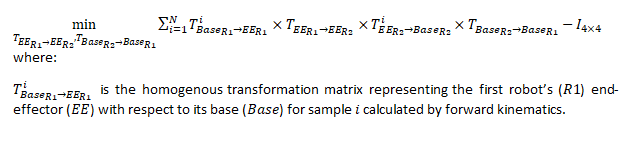
\includegraphics[width=\textwidth]{fig/handshake.png}
         \caption{Handshake calibration for base-to-base calibration. The two serial manipulators are rigidly attached and in admittance control mode.}
         \label{c1:fig:handshake}
     \end{subfigure}
     \hfill
     \begin{subfigure}[b]{0.3\textwidth}
         \centering
         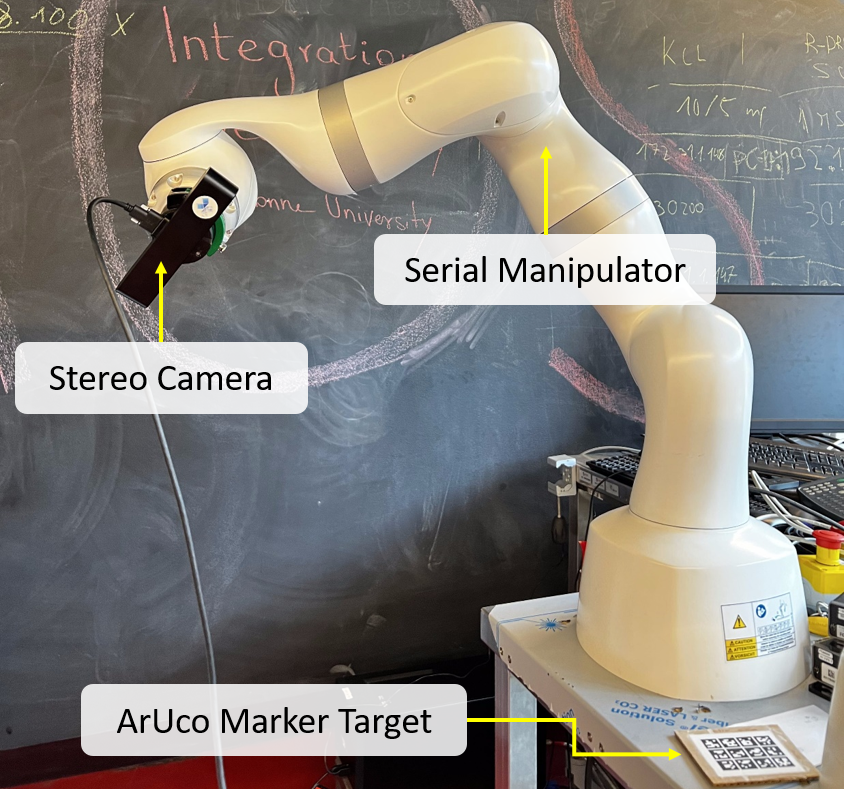
\includegraphics[width=\textwidth]{fig/eye_in_hand.png}
         \caption{Eye-in-hand calibration obtained through self-observation, where the serial manipulator observes itself.\\}
         \label{c1:fig:eye_in_hand}
     \end{subfigure}
     \hfill
     \begin{subfigure}[b]{0.3\textwidth}
         \centering
         \includegraphics[width=\textwidth]{fig/eye_to_hand.png}
         \caption{Eye-to-hand calibration in a dual serial manipulator setup to obtain base-to-base calibration.\\\\}
         \label{c1:fig:eye_to_hand}
     \end{subfigure}
    \caption{Calibration procedures. The proposed registration procedure, see \figref{c1:fig:calibration_pipeline}, is evaluated against alternative calibrations. The base-to-base calibration via eye-to-hand registration in (c) is compared against a handshake calibration in (a). The eye-in-hand calibration in (b) is compared against a classical calibration via an ArUco marker target, also (b). Refers to \secref{c1:sec:ex_vivo_experiments}.}
    \label{c1:fig:calibrations}
\end{figure}

The experimental setup is shown in \figref{c1:fig:handshake}-\figref{c1:fig:eye_to_hand}. We utilize two KUKA \gls{lbr} Med7 robots and control them via the \gls{lbr}-Stack (\appref{app:lbr_stack}) at a control rate of $100\,\text{Hz}$. For the handshake calibration, we deploy them in impedance control mode, see \secref{c1:sec:handshake_calibration}, for all other calibrations we use position control mode. The robots are mounted on a table and are fixed with respect to each other. By construction, their distance is $38\,\text{cm}$. For the camera we use a ZED 2i (Stereolabs, USA). We collect images and depth maps with a resolution of $448 \times 256$ at a frame rate of $15\,\text{Hz}$. For the depth estimation, we utilize the camera in neural depth perception mode.

Four baseline experiments are conducted, two regarding eye-in-hand and two regarding eye-to-hand calibration. For the eye-in-hand calibration, the camera is mounted to the robot via a GRIP G-SHW063 tool connector, see \figref{c1:fig:eye_in_hand}. For the baseline calibration experiments, see \secref{c1:sec:handshake_calibration}, we use a $3\times4$ ArUco marker target of square size $15.77\,\text{mm}$. $1259$ image-joint position correspondences are collected. For the proposed method, see \secref{c1:sec:simple_icp_registration}, we have the robot observe itself through the camera. We collect $1272$ image-joint position correspondences, but only use one. For the eye-to-hand calibration, the camera is put on an external tripod, see \figref{c1:fig:eye_to_hand}. $790$ image-joint position correspondences are collected, again only one is used. Robot 1 and robot 2 are calibrated and the base-to-base calibration is extracted, see \secref{c1:sec:proposed_calibration_procedure}. The base-to-base calibration is compared to a handshake calibration, see \figref{c1:fig:handshake} and \secref{c1:sec:handshake_calibration}. For the handshake, the robots are rigidly connected via a calibration fixture. $27700$ data points are collected of which $277$ are used for the calibration.

Finally, collision avoidant admittance control using the simple \gls{icp}, and exemplary base-to-base calibrations using the robust point-to-plane \gls{icp} are conducted. The collision avoidant admittance control is tested by moving the robots towards each other. The base-to-base calibration is evaluated visually.

\subsection{In-vivo Experiment}
\label{c1:sec:in_vivo_experiments}
\begin{figure}[tb]
    \centering
    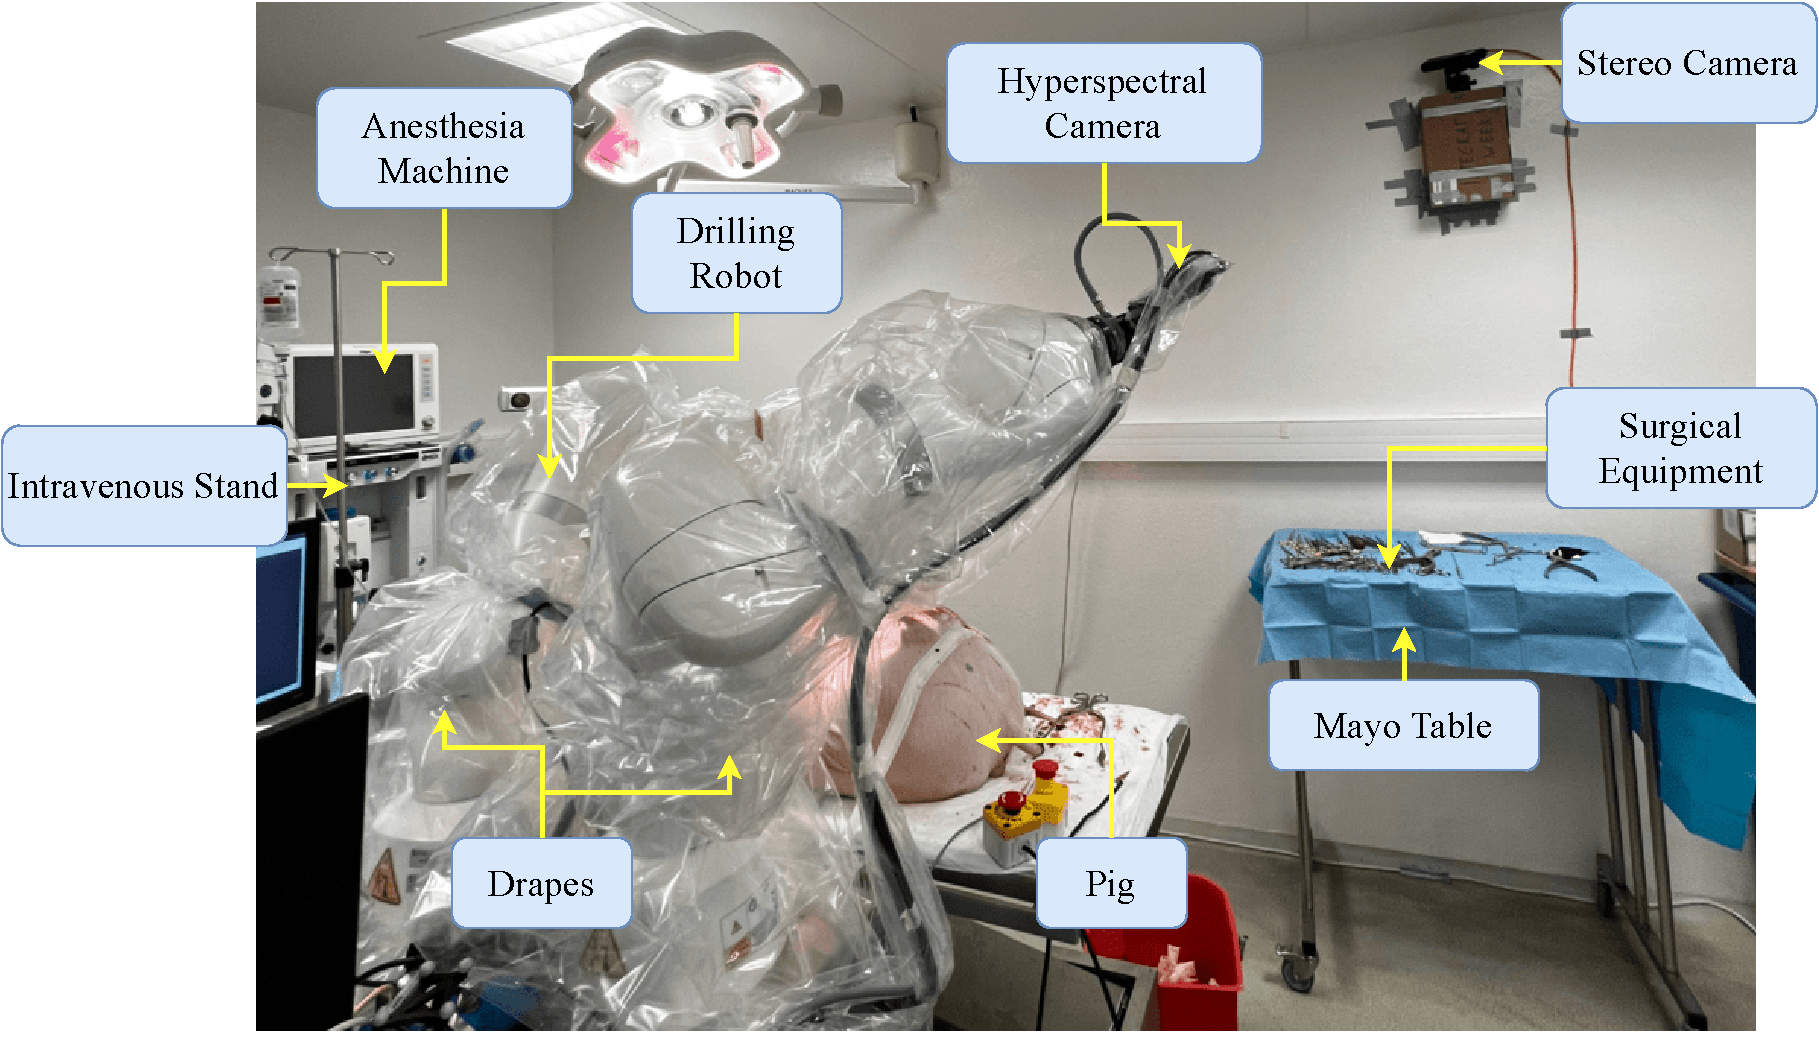
\includegraphics[width=0.8\textwidth]{chapter_1/img/in_vivo_setup.pdf}
    \caption{Clinical setup. A camera is mounted against a wall and both robots are registered using the proposed method of \secref{c1:sec:robust_icp}. Notably, the registration is performed prior to draping. Refers to \secref{c1:sec:in_vivo_experiments}.}
    \label{c1:fig:in_vivo_setup}
\end{figure}
To qualitatively verify the proposed method in a clinically relevant scenario, and to collect data, we conduct an in-vivo study. The primary goal of this experiment, however, is data collection. Given the registration, the recorded data can serve as ground truth for further marker-free registration despite draping. In the study, spine surgery is investigated, and in particular, robot-assisted pedicle screw placement. The pig is put under general anesthesia at all times. An overview of the setup is shown in \figref{c1:fig:in_vivo_setup}. Two KUKA \gls{lbr} Med7 R800 are deployed. Notably, both robots are draped, turning the proposed registration procedure unfeasible. Thus, registration is performed prior to draping, and neither the robots, nor the camera are moved thereafter. A ZED 2i stereo camera (Stereolabs, USA) is wall-mounted, so both robots and the surgical scene are in sight. We record stereo images and depth maps at a resolution of $540 \times 960$. Both robots are put into admittance control mode and are hand-guided into different configurations for sample collection.

\section{Results}
\label{c1:sec:results}
% TODO: cite optas ~\cite{optas} % for control of dual system

\subsection{Ex-vivo Results}
\label{c1:sec:ex_vivo_results}
\begin{figure}[tb]
     \centering
     \begin{subfigure}[b]{\textwidth}
         \centering
         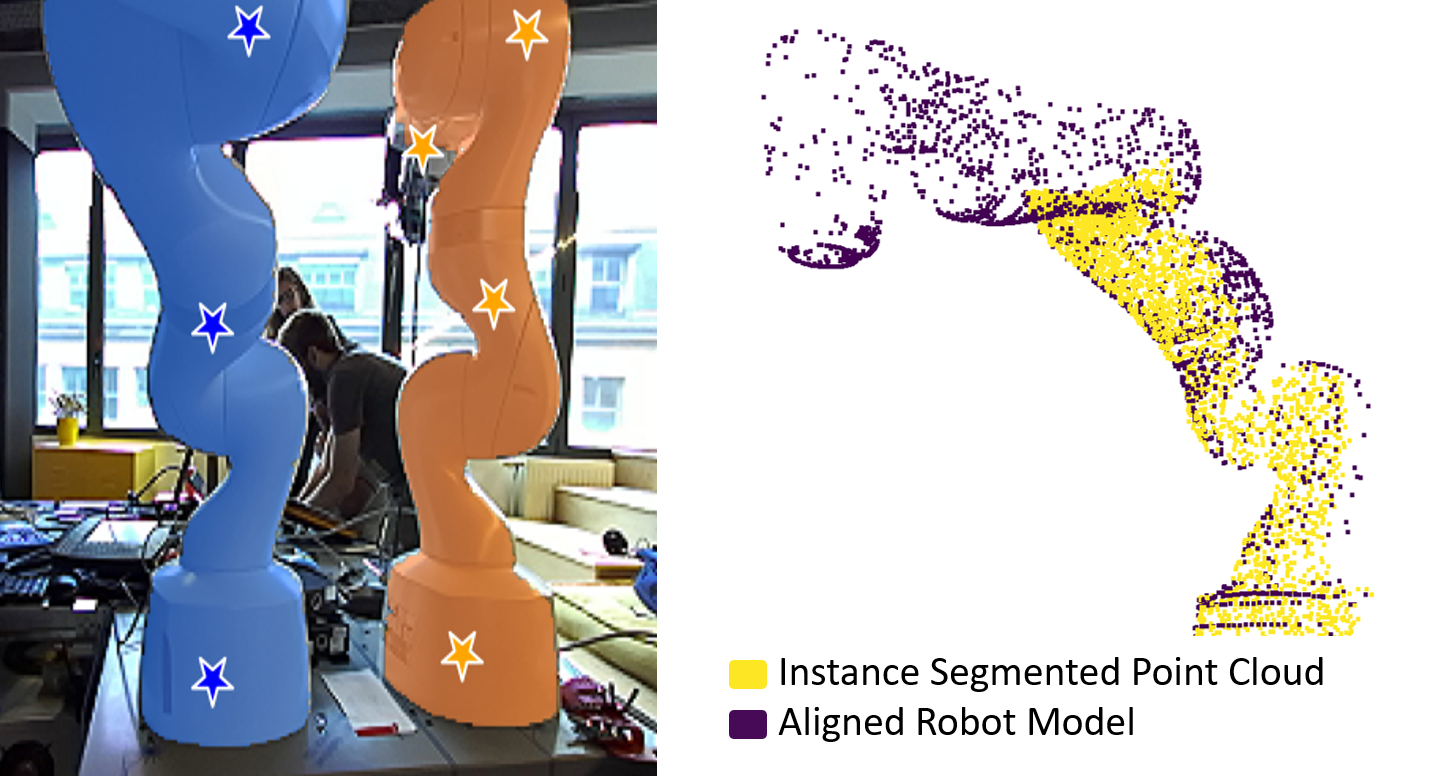
\includegraphics[width=0.6\textwidth]{img/visual_calibration/self_registration_combined_white.png}
         \caption{Eye-in-hand calibration, corresponding to \figref{c1:fig:eye_in_hand}. Left: Instance segmentation. The camera is mounted to robot one, highlighted through the blue mask. For visualization purposes, the image is rotated by $180^{\circ}$. Right: Point cloud to robot model registration.}
         \label{c1:fig:self_registration}
     \end{subfigure}
     \hfill
     \begin{subfigure}[b]{\textwidth}
         \centering
         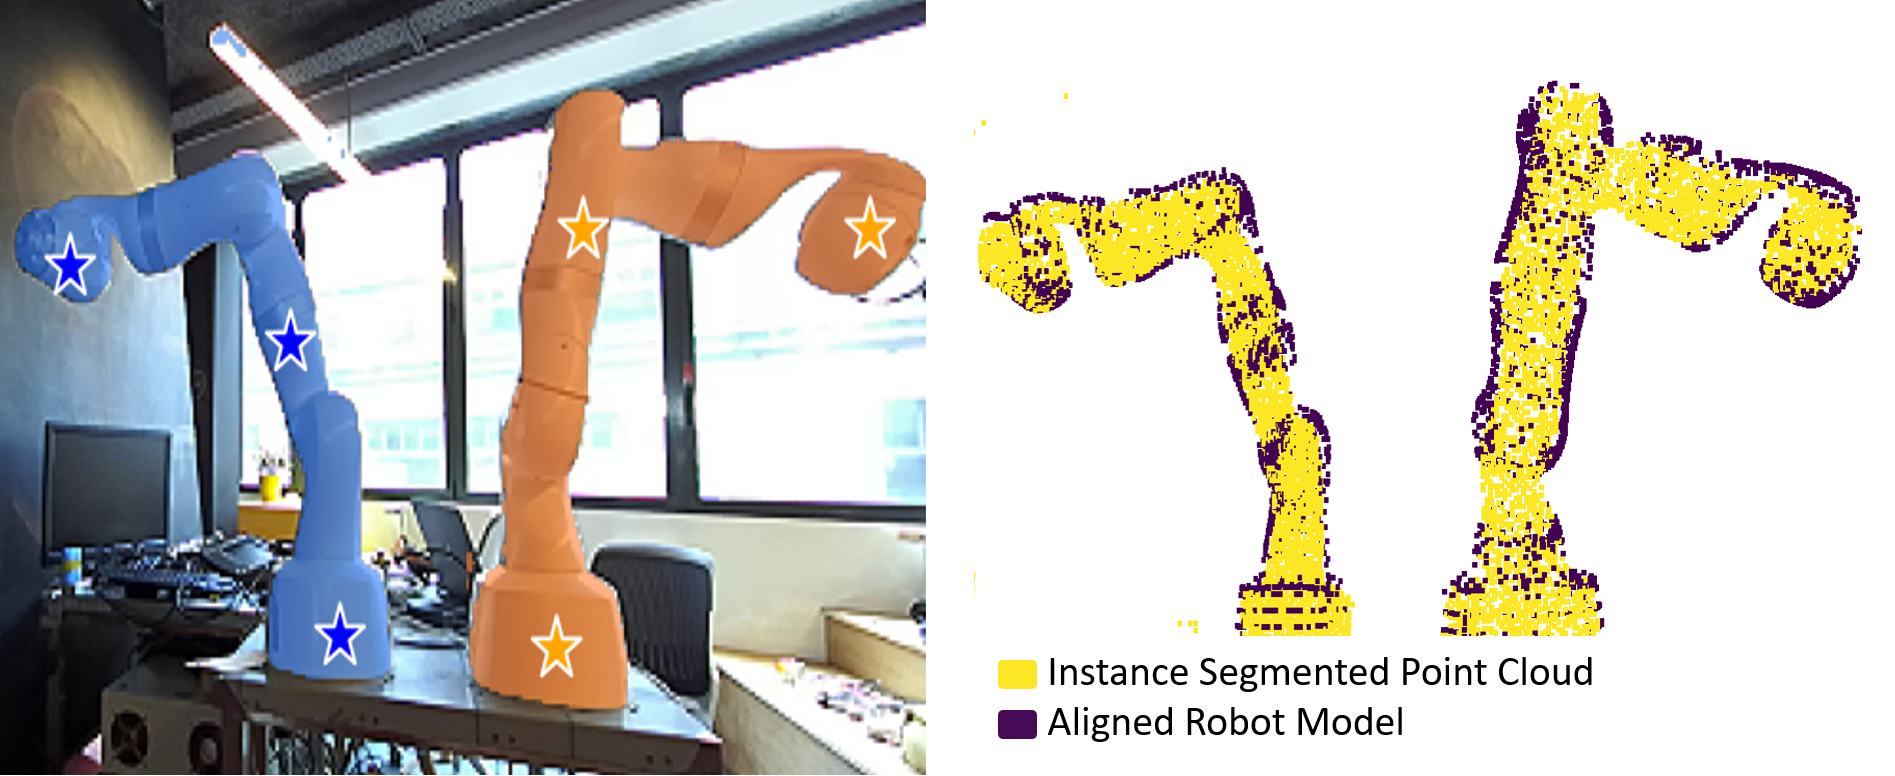
\includegraphics[width=0.6\textwidth]{img/visual_calibration/double_registration_combined_white.png}
         \caption{Eye-to-hand calibration, corresponding to \figref{c1:fig:eye_to_hand}. Left: Instance segmentation. The camera is mounted externally and observes robot one (blue mask) and robot two (orange mask). Right: Point cloud to robot model registration.}
         \label{c1:fig:double_registration}
     \end{subfigure}
     \caption{Ex-vivo eye-in-hand and eye-to-hand registrations. The instance-segmented point clouds $\mathbf{P}_\tau$ align well with the robot model $\mathcal{V}_\tau$. Refers to \secref{c1:sec:ex_vivo_results}.}
     \label{c1:fig:registration_results}
\end{figure}
\paragraph{Qualitative Baseline Results - Simple ICP} The registrations are shown in \figref{c1:fig:registration_results}. It can be observed that in both scenarios, i.e. eye-in-hand (\figref{c1:fig:self_registration}) and base-to-base via eye-to-hand (\figref{c1:fig:double_registration}), the segmentation via initial detection works well. The detections $\mathcal{F}_\tau$ are indicated through stars. Robot one and two can be clearly separated. This precise segmentation $\mathbf{S}_\tau$ results in an instance-segmented point cloud with very little outliers. The registration of the unaligned robot models $\mathcal{V}_\tau$ onto the instance-segmented point clouds $\mathbf{P}_\tau$ results in a visually compelling alignment (\figref{c1:fig:self_registration} - right - and \figref{c1:fig:double_registration} - right). Therein, the instance-segmented point clouds are visualized in yellow and the aligned robot models are shown in purple.

\begin{figure}[tbh]
    \centering
    \begin{subfigure}[b]{0.49\textwidth}
        \centering
        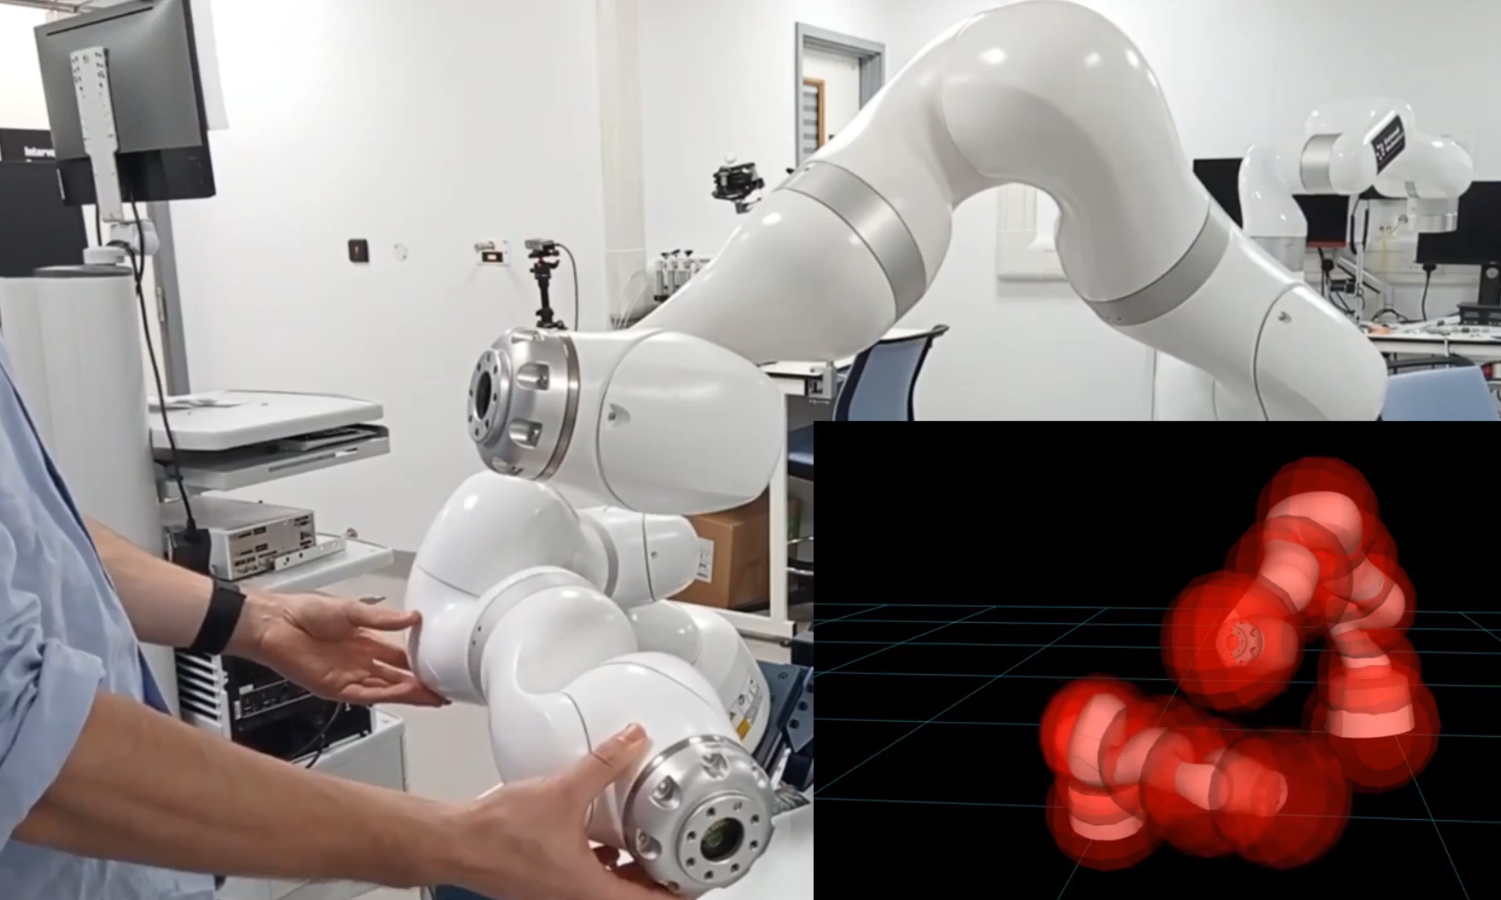
\includegraphics[width=\textwidth]{chapter_1/img/admittance_avoidance.png}
        \caption{Collision avoidant admittance control with spherical constraints, indicated in red.}
        \label{c1:fig:admittance}
    \end{subfigure}
    \begin{subfigure}[b]{0.49\textwidth}
        \centering
        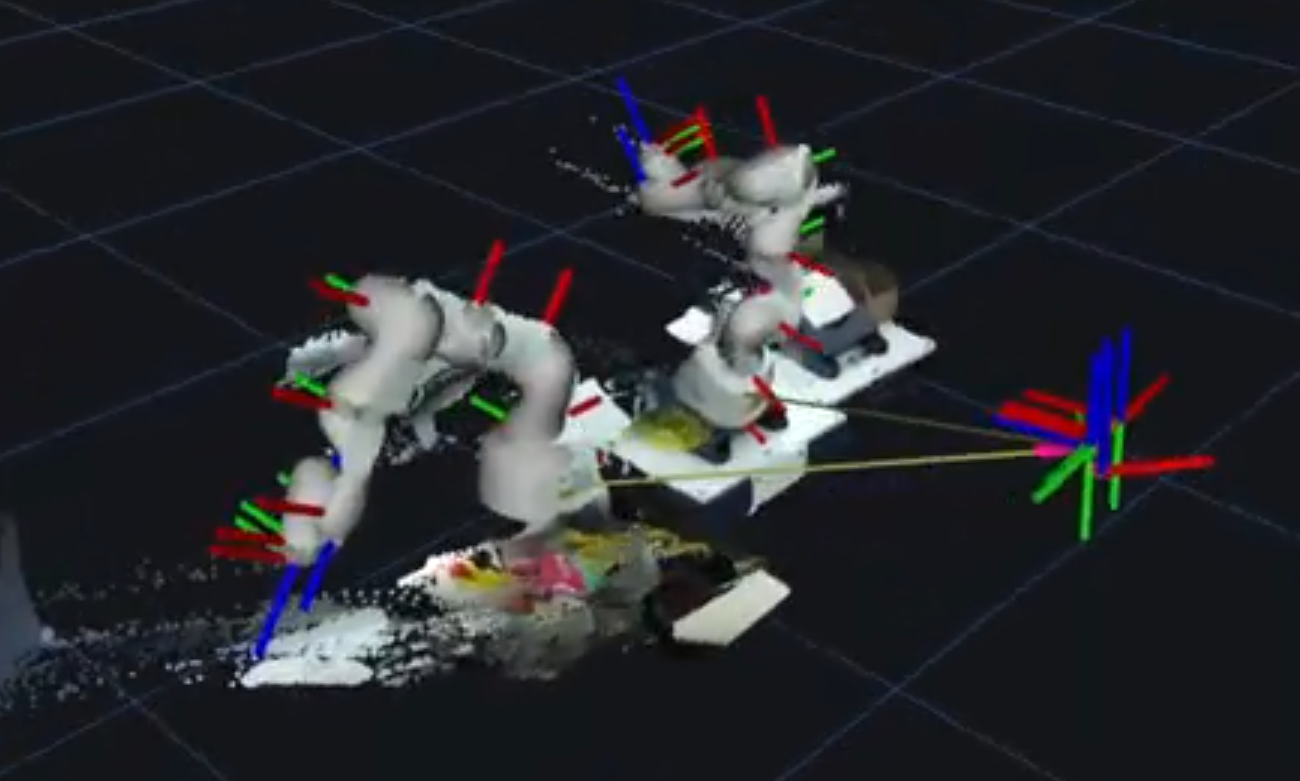
\includegraphics[width=\textwidth]{chapter_1/img/base_to_base_reg.png}
        \caption{Base-to-base registration and mesh overlay onto point cloud.}
        \label{c1:fig:base_to_base}
    \end{subfigure}
    \caption{Downstream applications of the eye-to-hand calibration. Refers to \secref{c1:sec:ex_vivo_results}. Videos are made available online\protect\footnotemark.}
    \label{c1:fig:downstream}
\end{figure}

\paragraph{Quantitative Baseline Results - Simple ICP} Quantitative results are summarized in \tabref{c1:tab:calibration_results}. For the eye-in-hand calibrations, it can be seen that the classical calibration procedure via ArUco markers deviates significantly from the manufactured values. This is most likely caused by noisy samples. In contrast, the proposed method, although single-shot, compares better with the expected manufactured values, which aligns well with the qualitative results in \figref{c1:fig:self_registration}. For the base-to-base calibration, it should be noted that the robots are fixed on a plain surface. The manufactured values can, therefore, be considered accurate. The proposed method yields precise results along the y-axis (distance between the robots), whereas the handshake deviates by $1\,\text{cm}$. The proposed method deviates $1\,\text{cm}$ along the z-axis from the manufactured and the handshake values. This dimension is the perpendicular offset to the surface plane. It can further be seen that the proposed method deviates slightly from the orientations of the handshake calibrations when compared to the manufactured values. The deviations might be caused by insufficiently synchronized images and joint states.

\paragraph{Qualitative Admittance Control - Simple ICP} Given the simple \gls{icp} registration results, refer \secref{c1:sec:simple_icp_registration}, we perform collision avoidant admittance control using the OpTas library~\cite{optas}. The spherical collision avoidance model is depicted in \figref{c1:fig:admittance}. Therein, the spherical constraints are indicated through red spheres are the links. As seen in the accompanying video (\figref{c1:fig:admittance}), the robot can be safely hand-guided in admittance control mode whilst avoiding collision within the spherical constraints.

\footnotetext{\\
Collision avoidant admittance control: \url{https://drive.google.com/file/d/14IhWxNsEmjGmVBnxTaMYIDQDOuo6Ihak/view?usp=sharing} \\
Base-to-base registration: \url{https://drive.google.com/file/d/18KFJyxDw6UiQ1N95tSQadi4TyGtBAQvc/view?usp=sharing}}

% single registration: \footnote[1]{Eye-to-hand calibration: \url{https://drive.google.com/file/d/1hN1wlVfnZ5D_zGIQtjSIh_OJwUPOeExR/view?usp=sharing}}

\paragraph{Qualitative Base-to-base Registration - Robust ICP} The qualitative results for the base-to-base via dual eye-to-hand calibration using the robust point-to-plane \gls{icp} of \secref{c1:sec:robust_icp} are shown in \figref{c1:fig:base_to_base}. In the accompanying video (\figref{c1:fig:base_to_base}), the robot meshes align well with the observed point cloud. Given these results, it is justified to deploy the method in the in-vivo scenario, see \secref{c1:sec:in_vivo_experiments} and \secref{c1:sec:in_vivo_results}.


% NOTE TO SELF:
% classical eye-in-hand calibration seems odd. Only 5 samples were used for registration
% the proposed solution to eye-in-hand seems solid

% classical eye in hand (huanyu)
% mean translation:
%  [ 0.    -0.042  0.026]
% std translation:
%  [0.159 0.07  0.041]
% mean rotation:
%  [  -1.057  -15.003 -167.708]
% std rotation:
%  [127.06   16.682   6.183]

% inverse of huanyu's
% translation:
%  [-0.015 -0.04  -0.024]
% euler:
%  [  2.199 -14.881 167.56 ]

% translation:
% proposed
% [-0.04  -0.056  0.085]
% euler_c_ee:
% [  0.461   2.212 146.686]

% inverse of proposed
% translation inverse:
% [ 0.    -0.069 -0.084]
% euler_c_ee inverse:
% [   1.601    1.595 -146.655]

% manufactured (zed)
% translation_inv:
%  [ 0.003 -0.06  -0.063]
% euler_inv:
%  [ 0.    -2.865  -156.000 ]

\subsection{In-vivo Results}
\label{c1:sec:in_vivo_results}
\begin{figure}[htb]
    \centering
    \begin{subfigure}[b]{0.49\textwidth}
        \centering
        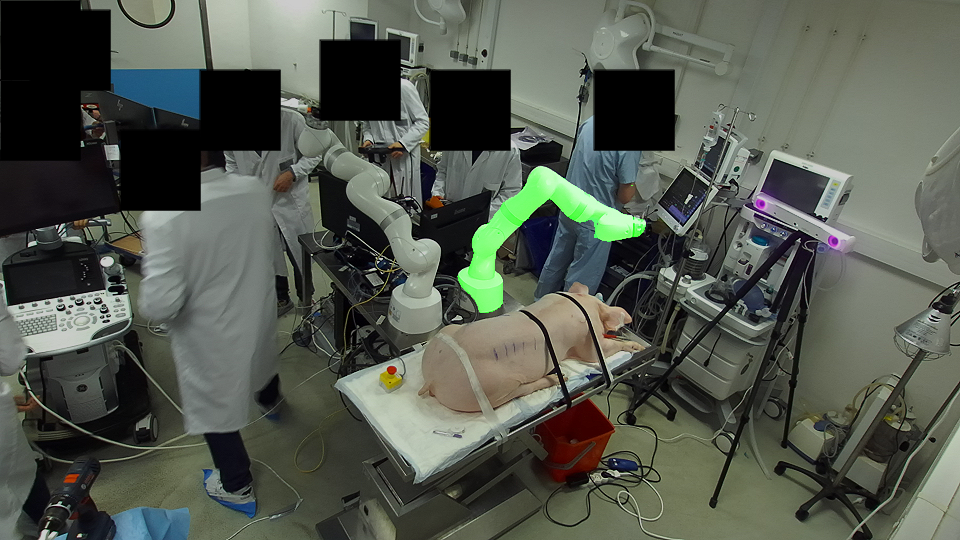
\includegraphics[width=\textwidth]{chapter_1/img/left_mask_overlay_0_anonymized.png}
    \end{subfigure}
    \begin{subfigure}[b]{0.49\textwidth}
        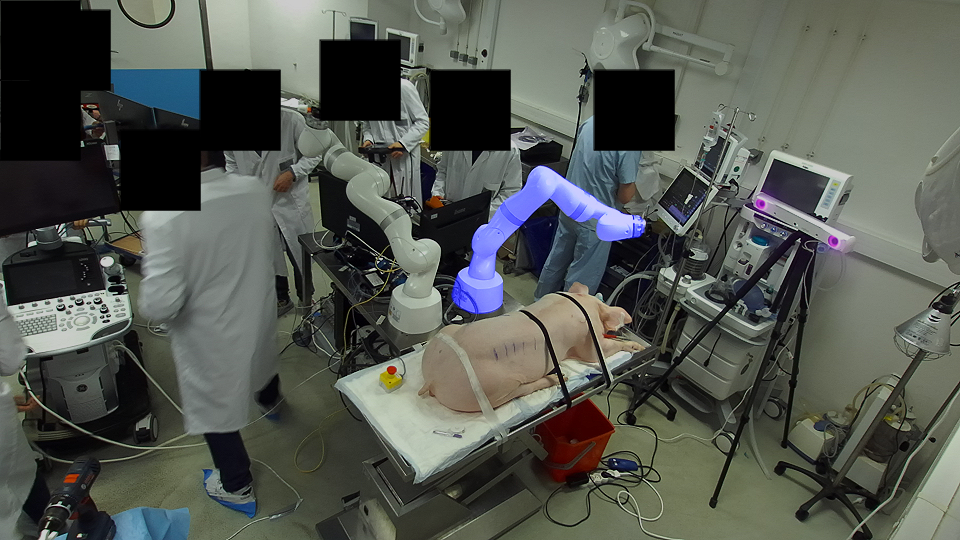
\includegraphics[width=\textwidth]{chapter_1/img/left_render_0_anonymized.png}
    \end{subfigure}
    \caption{Segmented robot (left) and rendered robot given registration (right). Visually, the render shows good alignment with the robot, hinting to an accurate calibration. Refers to \secref{c1:sec:in_vivo_results}.}
    \label{c1:fig:in_vivo_results}
\end{figure}
Initially, we collect 12 measurements for the drilling robot, and 14 measurements for the hyperspecral camera robot. These measurements include joint state, image, and depth correspondences. The positioning of both robots with respect to the camera is shown in \figref{c1:fig:in_vivo_setup}. Using these measurements, we perform a eye-to-hand calibration via the robust point-to-plane \gls{icp}, refer \secref{c1:sec:robust_icp}. 

For both robots, we collect a total of $4588$ stereo frames and depth maps with corresponding joint states, corresponding to about $10$ minutes of data at an average recorded frame rate of $8\,\text{fps}$. We collect an additional $5611$ correspondences for only one robot, either the drilling or the hyperspectral camera robot. This corresponds to about $7$ minutes of data at an average recorded frame rate of $13\,\text{fps}$.

Qualitative results of the registration for the drilling robot are shown in \figref{c1:fig:in_vivo_results}. Therein, and given the registration, we render the robot's meshes into the observed image. The render aligns well with the robot. It should be noted that the segmentation, \figref{c1:fig:in_vivo_results} - left, does not cover the entire robot but misses the bottom left bit. This was the case for all observed drilling robot mask and could be corrected through proper selection of points $\mathcal{F}_t$. For the camera robot on the other hand, we obtain close to perfect instance segmentations $\{\mathbf{S}_t\}$. Further exemplary segmentation masks and rendered masks, as well as difference images between segmentation and render, for both, the drilling robot and the camera robot, are shown in \figref{c1:fig:masks}.
\begin{figure}[tb]
    \centering
    \begin{subfigure}[b]{0.32\textwidth}
        \includegraphics[width=\textwidth]{chapter_1/img/hsi_left_mask_2.png}
        \caption{Camera robot: Segmentation.}
    \end{subfigure}
    \begin{subfigure}[b]{0.32\textwidth}
        \includegraphics[width=\textwidth]{chapter_1/img/hsi_left_render_mask_2.png}
        \caption{Camera robot: Rendered mask.}
    \end{subfigure}
    \begin{subfigure}[b]{0.32\textwidth}
        \includegraphics[width=\textwidth]{chapter_1/img/hsi_left_difference_2.png}
        \caption{Camera robot: L1-norm of segmentation and render.}
    \end{subfigure}
    \begin{subfigure}[b]{0.32\textwidth}
        \includegraphics[width=\textwidth]{chapter_1/img/drill_left_mask_1.png}
        \caption{Drilling robot: Segmentation}
    \end{subfigure}
    \begin{subfigure}[b]{0.32\textwidth}
        \includegraphics[width=\textwidth]{chapter_1/img/drill_left_render_mask_1.png}
        \caption{Drilling robot: Rendered mask.}
    \end{subfigure}
    \begin{subfigure}[b]{0.32\textwidth}
        \includegraphics[width=\textwidth]{chapter_1/img/drill_left_difference_1.png}
        \caption{Drilling robot: L1-norm of segmentation and render.}
    \end{subfigure}
    \caption{Example of segmented and rendered masks given the proposed registration procedure. Refer to \figref{c1:fig:in_vivo_setup} for nomenclature. Refers to \secref{c1:sec:in_vivo_results}.}
    \label{c1:fig:masks}
\end{figure}

For the total set of collected samples, we determine the average \gls{iou} between instance segmentations $\mathbf{S}_t$ and renders $\mathbf{R}_t$. Therein, the \gls{iou} is expressed through
\begin{equation}
    \text{IoU} = \frac{|\mathbf{S}_t \cup \mathbf{R}_t|}{|\mathbf{S}_t \cap \mathbf{R}_t|}
\end{equation}
The results are summarized in \tabref{c1:tab:iou}. As can be see, and as already visually observed in \figref{c1:fig:masks}, we find close to perfect average \gls{iou}. For the drilling robot, the average \gls{iou} is slightly worse than for the camera robot. This is because the instance segmentations $\mathbf{S}_t$ are systematically off by human annotator. Ideally, one should further investigate an error in Cartesian-space, in addition to pixel-space, to determine the true accuracy of the registration. Ground-truth data, however, is not available for this experiment. 
\begin{table}[tb]
\centering
\caption{Average \gls{iou} of segmented and rendered mask. Also compare to \figref{c1:fig:masks}. Refers to \secref{c1:sec:in_vivo_results}.}
\label{c1:tab:iou}
\begin{tabular}{@{}ll@{}}
\toprule
Robot         & \gls{iou} {[}a.u{]}   \\ \midrule
Camera (left)    & $0.92 \pm 0.01$ \\
Drilling (right) & $0.84 \pm 0.01$ \\ \bottomrule
\end{tabular}
\end{table}

%Drill:
%Average \gls{iou}: 0.8394461441870494
%Std \gls{iou}: 0.013859811026686823
%HSI:
%Average \gls{iou}: 0.9234094580204967
%Std \gls{iou}: 0.009454594255256406

\section{Conclusion and Future Work}% and outlook}
In this work we present a novel vision-based robot calibration procedure that unifies eye-in-hand and eye-to-hand calibration through casting them the same problem formulation. This is achieved by treating the robot as calibration target itself. In the eye-in-hand calibration scenario, the robot simply observes itself whilst in the eye-to-hand scenario the camera observes the robot from an external stand. The introduced formulation can further be used for rapid robot base-to-base calibrations.

\paragraph{Ex-vivo Summary} Promising qualitative results for the simple \gls{icp} (\secref{c1:sec:simple_icp_registration}) are presented in \figref{c1:fig:registration_results}. For both, eye-in-hand \figref{c1:fig:self_registration} and eye-to-hand \figref{c1:fig:double_registration}, the instance-segmented point cloud, as well as the robot model align well after registration. These qualitative observations also solidify through our quantitative comparisons against baselines, which are summarized in \tabref{c1:tab:calibration_results}. Whilst an error remains, the proposed method is much quicker, as it is single shot, is much safer to use, as opposed to the handshake calibration, and does not require any calibration targets, as opposed to the eye-in-hand calibration with ArUco target.

\paragraph{In-vivo Summary} For the in-vivo experiments \secref{c1:sec:in_vivo_experiments}, we deploy an improved version of the registration algorithm, see \secref{c1:sec:robust_icp}. Applicability to a clinical scenario was demonstrated, see \figref{c1:fig:in_vivo_setup}. Visually, we find close to pixel-perfect registrations, see \figref{c1:fig:in_vivo_results}. These visual observations are further confirmed through the measured average \gls{iou}, see \tabref{c1:tab:iou}. Whether the amount of collected data is sufficient for marker-free registration despite draping remains to be seen in future work.
% Given the vast amount of collected data and precise localization, see \secref{c1:sec:in_vivo_results}

\paragraph{Limitations} Shortcomings of this work are that a sufficient view of the robot is required to perform the calibration. In a surgical scenario, draping would cause an insufficient view. Consequentially, the calibration would have to be carried out as initialization and the robots would not be allowed to move afterwards. Clinically, however, it is necessary to drape the robots prior to moving them into position, i.e. prior to moving them into the sterile field. This work furthermore only considers robot-robot collision with full knowledge of the robots' states. Robot-staff / surgeon / equipment collisions would require a more general understanding of the scene, potentially even motion prediction.
%Another limitation is the simple \gls{icp} algorithm that was used in \algoref{alg:registration}, \secref{c1:sec:simple_icp_registration}. At times, convergence to local minima is observed.

\paragraph{Future Work} In this work we present a very simplistic registration procedure which already provides highly accurate registration results. These results could immediately be deployed to industrial robots, e.g. for collision avoidance purposes. In the clinical scenario, however, draping is an unsolved issue. Since draping does deform the observed point clouds significantly, the presented method would ultimately fail. However, vast amounts of data and precise localizations were collected as part of the in-vivo study, see \secref{c1:sec:in_vivo_results}. Future work could, therefore, use this data to develop marker-free registration procedures that might function despite draping.

%Improvements could focus on addressing the above, but also on exploring novel concepts. Instead of using a simple \gls{icp} algorithm for registration, one should investigate registration methods that deal well with registering partially observable points clouds. To address the partially observable point cloud issue, one might further move from single shot towards multi shot registration, where multiple robot configurations are observed. This should help improve the calibration accuracy. Research might find that optimal robot configurations exist for performing self-observation in eye-in-hand calibration and also for eye-to-hand calibration. The system might actively sense itself and its surroundings by minimizing uncertainty. Finally, it was omitted in this work that the presented method can also be used to have a robot observe itself and other surrounding robots. Active sensing could be deployed to have an observing robot understand its environment with high precision.

\begin{landscape}
    \begin{table}[htb]
    \caption{Calibration results using the proposed method (\secref{c1:sec:proposed_calibration_procedure}) and the baseline methods (\secref{c1:sec:handshake_calibration}). In addition to the calibration baselines, the table also lists manufactured values. The transforms are displayed in terms of translations $t_{x/y/z}$ and rotations in terms of Euler angles $r_{x/y/z}$.}
    \label{c1:tab:calibration_results}
    \centering
    \begin{tabular}{|l|l|l|l|l|l|l|l|l|}
    \hline
    Calibration Class             & Method       & Transform                                                                                                        & $t_x\,[\text{m}]$ & $t_y\,[\text{m}]$ & $t_z\,[\text{m}]$ & $r_x\,[^\circ]$ & $r_y\,[^\circ]$ & $r_z\,[^\circ]$ \\ \hline
    \multirow{3}{*}{Eye-in-hand}  & Manufactured & $\homogeneous{C}{E}$                                                                                  & $ 0.0$            & $-0.06$           & $-0.06$           & $ 0.0$          & $-2.9$          & $-145.0$        \\ \cline{2-9} 
                                  & ArUco        & $\homogeneous{C}{E}$                                                                                  & $ 0.0$            & $-0.04$           & $ 0.03$           & $-1.1$          & $-15.0$         & $-167.7$        \\ \cline{2-9} 
                                  & Proposed     & $\homogeneous{C}{E}$                                                                                  & $ 0.0$            & $-0.07$           & $-0.08$           & $ 1.6$          & $ 1.6$          & $-146.7$        \\ \hline
    \multirow{2}{*}{Base-to-base} & Manufactured & $\homogeneous{{B_2}}{{B_1}}$                                                                           & $ 0.0$            & $-0.38$           & $ 0.0$            & $0.0$           & $0.0$           & $ 0.0$          \\ \cline{2-9}
                                  & Handshake    & $\homogeneous{{B_2}}{{B_1}}$                                                                           & $-0.01$           & $-0.37$           & $ 0.0$            & $1.3$           & $0.3$           & $-0.6$          \\ \hline
    Base-to-base via eye-to-hand  & Proposed     & $\homogeneous{{B_2}}{{B_1}} = \homogeneous{C}{{B_2}}^{-1}\,\homogeneous{C}{{B_1}}$ & $-0.01$           & $-0.38$           & $-0.01$           & $1.7$           & $2.2$           & $-5.1$          \\ \hline
    \end{tabular}
    \end{table}
\end{landscape}

\graphicspath{{chapter_2}}
\chapter[Semi-autonomous Robotic Laparoscope]{Semi-autonomous Robotic Laparoscope under Remote Center of Motion Constraint}
\chaptermark{Visual Servoing}
\label{chap:robotic_endoscope}
\minitoc

\paragraph{Disclaimer} This \chapref{chap:robotic_endoscope} is an \textit{in extenso} reproduction of~\cite{huber2021homographybased}. Only \secref{c2:sec:introduction} was altered to highlight additional context within the scope of this thesis.

%published in~\cite{huber2021homographybased}

%% calibrations
%\secref{in:sec:camera_intrinsic_calibration}
%\secref{in:sec:eye_in_to_hand_calibration}

%% according
%\figref{in:fig:experimental_setup}

%% action execution
%\secref{in:sec:hypothesizing}
%\figref{in:fig:hypothesized_pipeline} $\hat{a}^*_t$
%\secref{in:sec:homography_based_camera_motion_formulation}


\newpage

% Contributes ...

% \section{Introduction}
% When compared to open surgery, \acrshort{mis} takes place under endoscopic guidance and offers improved cosmetics, less blood loss, shorter recovery times and reduced cost~\cite{vitiello2012emerging}. In a traditional \acrshort{mis} setup, the surgeon is supported by an assistant who guides the endoscope. Although this task is conceptually simple, it requires trained personnel, which introduces cost~\cite{horgan2001robots}. The assistant surgeon exhibits tremor, suffers fatigue, and can be prone to communication failures~\cite{horgan2001robots, palep2009robotic, li2020accelerated}. 

% Several robotic endoscope holders, such as AESOP~\cite{unger1994aesop}, ViKY~\cite{long2007development}, and EndoAssist~\cite{gilbert2009endoassist}, have been developed to address these shortcomings. Research in~\cite{aiono2002controlled} and~\cite{voros2010viky} showcased a reduction in the intervention time. While robotic endoscope holders can facilitate improvements, they introduce additional workload to the surgeon. With the advance of automated surgical systems this additional workload can be reduced~\cite{moustris2011evolution}. Therefore, different methods to automate endoscopic camera motion were explored. 

% Alongside automation via kinematic data, visual servoing, i.e. control through images, is considered a promising alternative, as it provides intra-operative feedback~\cite{pandya2014review} and is less prone to errors from model mismatch~\cite{azizian2014visual}. In semi-autonomous setups, such as gaze or voice control~\cite{taniguchi2010classification}, visual servoing can robustly reflect a surgeon's intent and respect anatomical constraints or facilitate full autonomy.

% Visual servoing approaches that satisfy a \acrshort{rcm} constraint can be split into methods that rely on a mechanical \acrshort{rcm} and methods that rely on a programmable \acrshort{rcm}. There has been less research on visual servoing with programmable \acrshort{rcm} because of robot singularities and constraints on the robot positioning, however, in contrast to a mechanical \acrshort{rcm}, a programmable \acrshort{rcm} can be adapted in real-time, and the robot, with which the programmable \acrshort{rcm} is achieved, can be used for multiple purposes~\cite{kuo2012kinematic}, for example in open surgery. Existing methods with mechanical \acrshort{rcm}, and programmable \acrshort{rcm}, will be detailed in \secref{c2:sec:mech_rcm}, and \secref{c2:sec:prog_rcm}, respectively.
%\begin{figure}
%    \centering
%    \includegraphics[width=\textwidth]{img/labeled_setup_compressed.png}
%    \caption{Robotic setup. A Storz Endocameleon Hopkins Telescope, which provides a light source port and a camera attachment point, is mounted to a KUKA LBR Med 7 R800 robot via a 3D printed clamp. The robotic system undergoes image-based control to reach desired views of the surgical scene and simultaneously pivots around a programmable \acrshort{rcm}.}
%    \label{c2:fig:setup}
%\end{figure}

%\subsection{with Mechanical \acrshort{rcm}}
%\subsection{Visual Servoing with Mechanical \acrshort{rcm}}
%\label{c2:sec:mech_rcm}
%Examples of approaches that use a mechanical \acrshort{rcm} are~\cite{omote1999self}, where a visual servo controls the position of a marked forceps in image space. In~\cite{agustinos2014visual, voros2007automatic}, the tool entry point is exploited to find the tool tip in image space and to center it via visual servoing. Another common scheme is to alter the camera's zoom based on the surgical tools' distance, which was first presented in~\cite{king2013towards}, where the tools are tracked with markers. Research in~\cite{eslamian2020development, mariani2020experimental, dascan}, based on ~\cite{Eslamian2016TowardsTI, eslamian2017autonomous}, adjusts the camera's distance in this manner. They align the camera's optical axis with the line that spans from \acrshort{rcm} to the tools' center point. Such an approach requires a complicated registration procedure. In~\cite{abdelaal2020orientation}, Abdelaal \emph{et al.} also adjust the camera's distance to the surgical scene based on the tool distance, but they align the camera's optical axis with the scene's surface normal, which is made possible by their 6 DOF endoscope. Yu \emph{et al.}~\cite{yu2016automatic} adjust the field of view's width based on tool distance. In~\cite{ma2019autonomous}, Ma \emph{et al.} deploy a visual servo to center a marked tool by incorporating depth information, which they extract from camera and tool motion. In~\cite{ma2020visual}, they extend this work into a quadratic program in which they constrain the camera's distance with respect to the tools and the tool position in the image plane, whilst minimizing the joint velocities. They rely on stereoscopic images for depth information.

%\subsection{Visual Servoing with Programmable \acrshort{rcm}}
%\label{c2:sec:prog_rcm}
%Multi-purpose serial manipulators can achieve a \acrshort{rcm} programmatically. In~\cite{osa2010framework}, Osa \emph{et al.} adapt the interaction matrix to account for the \acrshort{rcm} constraint, which they then use to control a point in image space. The authors in~\cite{aghakhani2013task} design a composite Jacobian method that integrates a \acrshort{rcm} objective with a task function that defines an error on points in image space. Yang \emph{et al.} in~\cite{yang2019adaptive} also design a Jacobian gain controller that enforces the tip of a tool to reside within a defined region. They additionally request the endoscope to extend the surgeon's natural line of sight. In~\cite{li2020accelerated}, Li \emph{et al.} introduce the \acrshort{rcm} and a visual error via the image Jacobian as constraints to a quadratic problem that aims at satisfying these constraints whilst minimizing the joint velocities.

% option A:
% Automation in General
% Automation with mechanical \acrshort{rcm}, Automation with programmable \acrshort{rcm}
% Add other kinematic papers (\cite{weede2011intelligent})
% Add sun
% Move kinematic shortcomings to "Limitations of current approaches"

% option B:
% Remove "kinematic" VS from Mech \acrshort{rcm}
% Add short list of kinematic approaches
% Add collection of visual servo with mechanical rcm
% Add sun
% Highlight shortcomings

%\cite{weede2011intelligent}   % Markov
%\cite{sun2020development}     % kinematic -> image space velocity, center tool
%\cite{sun2020adaptive}        % mechanical rcm, adjust angle based on fusion of kinematic and visual data (stereoscopic)
%\cite{sun2020visual}          % (estimate depth based on laparoscopic motion)

\section{Introduction}
\label{c2:sec:introduction}
As was discussed in \secref{in:sec:automation_approaches}, vision-based automation offers a shared domain between \acrshort{mis} and \acrshort{rmis}, see \figref{in:fig:shared_domain}. The shared domain is essential for the realization of the proposed imitation learning pipeline, see \figref{in:fig:hypothesized_pipeline}, without which imitating human experts with a robot might be difficult. Many other works for laparoscopic camera motion automation in the image domain exist, and were reviewed in \secref{in:sec:rule_based_approaches}, yet most of them adhere to the tool following assumption, which we evidently rejected therein. It is, however, a priori not obvious how else one could formulate a visual servo instead. In this publication, we argue that previous works are missing the bigger picture. We take a step back and attempt to shift the focus from tools to organs by treating the visual servoing task as a registration problem.

Arguably, registration might not seem a good automation paradigm, since surgical scenes are dynamic and change over time, which is likely why no one attempted it. Therefore, it is important to understand the context within this work. We are ultimately not interested in global registration but registration of temporal changes from $\hat{s}_t$ to $\hat{s}_{t+1}$, i.e. desired image space actions $\hat{a}^*_t$, that is the human expert policy. Now, prior to predicting actions through imitation learning, \chapref{chap:camera_motion_extraction}, and \chapref{chap:camera_motion_prediction}, thus deviating from learning auxiliary tasks, refer \secref{in:sec:auxiliary_tasks}, we choose to proof that, indeed, the hypothesized actions, i.e. homographies, refer \secref{in:sec:homography_based_camera_motion_formulation}, may be executed under the \acrshort{rcm} constraint. In this work, we contribute exactly that. We formulate an image-based visual servo for executing the embodiment-invariant action $\hat{a}^*_t$. Deviating from the dominant methods, the proposed image-based visual servo requires neither explicit tool and camera positions nor any explicit image depth information, whilst satisfying a \acrshort{rcm} constraint on a serial arm manipulator, see \figref{in:fig:experimental_setup}, thereby obeying \secref{in:sec:automation} - System Considerations.

Built on top of the image-based visual servo, we propose a semi-autonomous scheme, where actions $\hat{a}^*_t$ are generated by the user through selecting target views. The approach allows a user to build a graph of desired views, from which, once built, views can be manually chosen and automatically servoed to irrespective of robot-patient frame transformation changes. This scheme targets level three autonomy, refer \secref{in:sec:foreword}, as we gradually pave the way towards level five autonomy in the remainder of this thesis.

%The proposed method relies on homography-based image registration, which changes the automation paradigm from point-centric towards surgical-scene-centric approach. It simultaneously respects a programmable Remote Center of Motion (\acrshort{rcm}). 

%We evaluate our method on an abdominal phantom and provide an open source ROS Moveit integration for use with any serial manipulator\footnote[3]{ \url{https://github.com/RViMLab/h_rcm_vs_ws.git}}. A video is provided\footnote[4]{\label{foot:vid}\url{https://drive.google.com/file/d/1UCr__R2_7xit6TTq3T9pTIEg1fMsfT3j/view?usp=sharing}}.
%\end{abstract}

%\begin{abstract}
% The dominant endoscope manipulation automation approaches in Minimally Invasive Surgery (MIS) rely on point positions w.r.t. the camera frame to infer a control policy
%The dominant visual servoing approaches in Minimally Invasive Surgery (MIS) follow single points or adapt the endoscope's field of view based on the surgical tools' distance. These methods rely on point positions with respect to the camera frame to infer a control policy. 

\subsection{Limitations of Current Approaches and Contributions}
The majority of existing methods rely on the tool distance to infer a control law. Only in~\cite{ma2019autonomous, ma2020visual, aghakhani2013task, yang2019adaptive, li2020accelerated, osa2010framework}, the position of arbitrary points w.r.t. the camera frame is fed back to the robot. All of the existing methods rely on relative positions, which either requires tool and camera positions or depth images. Position data might only be accessible in a fully robotic setup and image depth is difficult to estimate in a dynamic surgical environment from a monocular camera. Stereoscopic images are usually not available in robot assisted surgery.

Our paper addresses the above limitations with the following contributions:
\begin{itemize}
    \item We introduce a visual servo that navigates towards desired images rather than towards points.
    \item We formulate a visual servo control law that depends neither on explicit tool and camera positions nor on depth information.
\end{itemize} 
These are achieved with a programmable \acrshort{rcm}, as it, in contrast to a mechanical \acrshort{rcm}, is more flexible. 

This paper is structured as follows. In \secref{c2:sec:methods}, we introduce the necessary theoretical background and the derivation of the proposed visual servoing task. In \secref{c2:sec:experimental_setup}, we explain implementation details and the robotic setup. Results are provided in \secref{c2:sec:results}, and conclusions in \secref{c2:sec:conclusions}.

\section{Methods}
\label{c2:sec:methods}
%In this section,
Here, we first introduce the composite Jacobian for control in \secref{c2:sec:task_rcm}. Then, we extend it by a novel homography-based task function in \secref{c2:sec:homography_task}, and describe the processing pipeline in \secref{c2:sec:pipe}. In the following, scalars are depicted by lower case letters, vectors through bold lower case letters, and matrices as bold upper case letters. A point $x$ is described with respect to frame F as $^\text{F}\mathbf{x}$.

\subsection{Task Control with Remote Center of Motion Objective}
\label{c2:sec:task_rcm}
For the task control with \acrshort{rcm} objective, we follow the derivation of Aghakhani \emph{et al.} ~\cite{aghakhani2013task}. Therefore, as schematically shown in \figref{c2:fig:schematic}, an open kinematic chain is attached to reference frame W. An endoscope is attached to the chain. It originates at position $^\text{W}\mathbf{x}_i$ and has its camera frame at position $^\text{W}\mathbf{x}_{i+1}$. The endoscope enters the patient through the trocar at position $^\text{W}\mathbf{x}_\text{trocar}$. The \acrshort{rcm} position $^\text{W}\mathbf{x}_\text{RCM}$ is required to lie along the line connecting $^\text{W}\mathbf{x}_i$ to $^\text{W}\mathbf{x}_{i+1}$, hence
\begin{equation}
^\text{W}\mathbf{x}_\text{RCM} = ^\text{W}\mathbf{x}_i+\lambda\left(^\text{W}\mathbf{x}_{i+1} - ^\text{W}\mathbf{x}_i\right),
\label{c2:eq:lambda}
\end{equation}
where the scalar $\lambda \geq 0$ is proportional to the entry depth. $\lambda = 0$ corresponds to maximal insertion. The endoscope's translational velocity at position $^\text{W}\mathbf{x}_\text{RCM}$ has to remain zero for the endoscope to reside at the trocar $^\text{W}\mathbf{x}_\text{trocar}$. It was derived in~\cite{aghakhani2013task} as
\begin{equation}
    ^\text{W}\dot{\mathbf{x}}_\text{RCM} = \begin{bmatrix}\mathbf{J}^v_i + \lambda(\mathbf{J}^v_{i+1}-\mathbf{J}^v_i)\\ ^\text{W}\mathbf{x}_{i+1} - ^\text{W}\mathbf{x}_i\end{bmatrix}^\text{T}\begin{bmatrix}\dot{\mathbf{q}} \\ \dot{\lambda}\end{bmatrix},
    \label{c2:eq:dx_RCM}
\end{equation}
where $\mathbf{J}^v_i$, $\mathbf{J}^v_{i+1}$ are the Jacobians' top three rows, therefore the translational parts, corresponding to points $^\text{W}\mathbf{x}_i$, $^\text{W}\mathbf{x}_{i+1}$ w.r.t. the world frame, $\dot{\mathbf{q}}$ are the instantaneous joint velocities, and $\dot{\lambda}$ is the rate of change of entry depth. \eqref{c2:eq:dx_RCM} can be rewritten as
\begin{equation}
    ^\text{W}\dot{\mathbf{x}}_\text{RCM} = \mathbf{J}_\text{RCM}\begin{bmatrix}\dot{\mathbf{q}} \\ \dot{\lambda}\end{bmatrix}.
    \label{c2:eq:dx_RCM_short}
\end{equation}
Expanding on~\cite{aghakhani2013task}, we introduce a feedback to $\lambda$ by projecting the trocar position $\mathbf{x}_\text{trocar}$ onto the endoscope via
\begin{equation}
    \lambda = \frac{(^\text{W}\mathbf{x}_{i+1} - ^\text{W}\mathbf{x}_i)^\text{T}(^\text{W}\mathbf{x}_\text{trocar}-^\text{W}\mathbf{x}_i)}{||^\text{W}\mathbf{x}_{i+1}-^\text{W}\mathbf{x}_i||_2^2}.
\end{equation}
\eqref{c2:eq:dx_RCM_short} can be further extended by a task as follows
\begin{equation}
    \begin{bmatrix}\dot{\mathbf{t}} \\ ^\text{W}\dot{\mathbf{x}}_\text{RCM}\end{bmatrix} =
    \begin{bmatrix}\mathbf{J}_\text{t} & \mathbf{0}_{n_\text{t}\times 1} \\ \multicolumn{2}{c}{\mathbf{J}_\text{RCM}}
    \end{bmatrix}
    \begin{bmatrix}\dot{\mathbf{q}}\\\dot{\lambda}\end{bmatrix},
    \label{c2:eq:task_jac}
\end{equation}
where $\dot{\mathbf{t}}$ is the task velocity with task dimension $n_\text{t}$ and $\mathbf{J}_\text{t}$ is the task Jacobian. \eqref{c2:eq:task_jac} can be turned into a PID controller
\begin{equation}
    \centering
    \begin{bmatrix}
        \dot{\mathbf{q}}\\
        \dot{\lambda}
    \end{bmatrix} = 
    \mathbf{J}_\text{cp}^{\dagger}
    \left(
        \mathbf{K}^\text{p}
        \begin{bmatrix}
            \mathbf{e}_\text{t}^\text{p}\\
            ^\text{W}\mathbf{e}_\text{RCM}^\text{p}
        \end{bmatrix} +
        \mathbf{K}^\text{i}
        \begin{bmatrix}
            \mathbf{e}_\text{t}^\text{i}\\
            ^\text{W}\mathbf{e}_\text{RCM}^\text{i}
        \end{bmatrix} +
        \mathbf{K}^\text{d}
        \begin{bmatrix}
            \mathbf{e}_\text{t}^\text{d}\\
            ^\text{W}\mathbf{e}_\text{RCM}^\text{d}
        \end{bmatrix}
    \right),
    \label{c2:eq:pid}
\end{equation}
where $\mathbf{J}_\text{cp}^{\dagger}$ is the pseudo-inverse of the composite Jacobian from (\eqref{c2:eq:task_jac}), $\mathbf{e}^{\text{p}/\text{i}/\text{d}}_t$ and $^\text{W}\mathbf{e}^{\text{p}/\text{i}/\text{d}}_\text{RCM}$, are the proportional, integral, and differential errors for the task and the \acrshort{rcm}, respectively, and $\mathbf{K}^{\text{p}/\text{i}/\text{d}}$ are the diagonal gain matrices. Therein, $^\text{W}\mathbf{e}_\text{RCM}^{\text{i}/\text{d}}$ are computed as the integral, and the differential of the proportional error $^\text{W}\mathbf{e}_\text{RCM}^\text{p} = ^\text{W}\mathbf{x}_\text{trocar} - ^\text{W}\mathbf{x}_\text{RCM}$. 

In the following section, we introduce a homography-based visual servoing task.

\subsection{Homography-based Visual Servoing Task}
\label{c2:sec:homography_task}

\begin{figure}[tb]
\centering
\includegraphics[width=0.7\textwidth]{img/h_rcm_vs_fig.pdf}
\caption{Schematic illustration of the setup: The axes' RGB coloring corresponds to XYZ, respectively. A serial manipulator is connected to the world frame W. The endoscope spans from $^\text{W}\mathbf{x}_i$ to $^\text{W}\mathbf{x}_{i+1}$ and it enters the trocar, which lies at $\mathbf{x}_\text{trocar}$. The camera rotates around the \acrshort{rcm} $^\text{W}\mathbf{x}_\text{RCM}$ and its entry depth is proportional to $\lambda \geq 0$.  The camera observes the surgical scene (pink) from different frames $\text{C}$ and $\text{C}^*$.}
\label{c2:fig:schematic}
\end{figure}

% \begin{landscape}
\begin{figure}[tb]
\centering
\includegraphics[width=\textwidth]{img/h_rcm_vs_pipeline_real_view.pdf}
\caption{Processing pipeline. A surgeon manually controls the robot through a GUI, collecting desired views along the way. The images are pre-processed, and a graph of desired views is built in the background by the homography generation node. Once built, the surgeon selects desired views through the GUI, which triggers a shortest path finding from the current vertex (yellow), to the desired one (pink), and the execution of subsequent homography estimations that lead to the target.}
\label{c2:fig:pipe}
\end{figure}
% \end{landscape}

Suppose point $^\text{W}\mathbf{X}$ is projected from a plane, i.e. the surgical scene, onto normalized coordinates $\mathbf{m}^*$ in camera frame $C^*$, see \figref{c2:fig:schematic}, via
\begin{equation}
    ^{\text{C}^*}\mathbf{m}^* = \frac{1}{^{\text{C}^*}Z^*}\begin{bmatrix}^{\text{C}^*}X^*&^{\text{C}^*}Y^*&^{\text{C}^*}Z^*\end{bmatrix}^\text{T},
\end{equation}
which means it is observed by the camera as
\begin{equation}
    ^{\text{C}^*}\mathbf{p}^* = \mathbf{K}^{\text{C}^*}\mathbf{m}^*,
\end{equation}
in pixel coordinates $^{\text{C}^*}\mathbf{p}^*=\begin{bmatrix}u^*&v^*&1\end{bmatrix}^\text{T}$, with the camera's intrinsic parameters $\mathbf{K}$. Should the camera move under rotation $\mathbf{R}$ and translation $\mathbf{t}$, the points in normalized coordinates will change according to a homography $\mathbf{H}$ such that~\cite{benhimane2006homography}
\begin{equation}
    \frac{^{\text{C}}Z}{^{\text{C}^*}Z^*}{^{\text{C}}\mathbf{m}} = \mathbf{H}^{\text{C}^*}\mathbf{m}^*
\end{equation}
In pixel coordinates this can be written as
\begin{equation}
    \frac{^{\text{C}}Z}{^{\text{C}^*}Z^*}{^{\text{C}}\mathbf{p}} = \mathbf{G}{^{\text{C}^*}\mathbf{p}}^*,
\end{equation}
with the projective homography $\mathbf{G}$, for which the following relation holds
\begin{equation}
    \mathbf{H} = \mathbf{K}^{-1}\mathbf{G}\mathbf{K}.
    \label{c2:eq:h_norm}
\end{equation}

As shown in~\cite{benhimane2006homography}, the task error $^\text{C}\mathbf{e}_{\text{t}'} = \begin{bmatrix}^\text{C}\mathbf{e}_v & ^\text{C}\mathbf{e}_\omega\end{bmatrix}^\text{T}$ that urges to minimize the distance between the desired projection of $^\text{W}\mathbf{X}$, $^{\text{C}^*}\mathbf{m}^*$, and the current one $^\text{C}\mathbf{m}$, can be obtained purely from the homography that relates those points in normalized coordinates via
\begin{equation}
    \begin{split}
        ^\text{C}\mathbf{e}_v & = (\mathbf{H} - \mathbf{I})^{\text{C}^*}\mathbf{m}^*\\
        \left[^\text{C}\mathbf{e}_\omega\right]_\times & = \mathbf{H} - \mathbf{H}^\text{T},
    \end{split}
    \label{c2:eq:dc}
\end{equation}
where $\left[^\text{C}\mathbf{e}_\omega\right]_\times$ is the skew symmetric matrix of $^\text{C}\mathbf{e}_\omega$. The task error $^\text{C}\mathbf{e}_{\text{t}'}$ is described in body coordinates. It can be transferred to the world frame W through rotation, which is proportional to camera frame's instantaneous velocity
\begin{equation}
    \begin{bmatrix}^\text{W}\mathbf{R}_\text{C} & \mathbf{0} \\ \mathbf{0} & ^\text{W}\mathbf{R}_\text{C}\end{bmatrix}{^\text{C}\mathbf{e}_{\text{t}'}} = ^\text{W}\mathbf{e}_{\text{t}'} \sim \mathbf{J}_{i+1}\dot{\mathbf{q}}
    \label{c2:eq:body}
\end{equation}
where $^\text{W}\mathbf{R}_\text{C}$ is the rotation of the camera frame with respect to the world frame, and $\mathbf{J}_{i+1}$ is the camera frame's Jacobian, including its rotational contributions. Only 4 DOF can be controlled at a time after imposing the \acrshort{rcm}, which constraints 2 DOF. To capture this, we introduce operator $\mathbf{P}$ that projects the camera frame body velocity onto the remaining DOF. Together with \ (\eqref{c2:eq:body}), this yields
\begin{equation}
    \mathbf{P}_{a/b}{^\text{C}\mathbf{e}_{\text{t}'}} = ^\text{C}\mathbf{e}_{\text{t}_{a/b}} \sim \mathbf{P}_{a/b} \begin{bmatrix}^\text{C}\mathbf{R}_\text{W} & \mathbf{0} \\ \mathbf{0} & ^\text{C}\mathbf{R}_\text{W}\end{bmatrix}\mathbf{J}_{i+1}\dot{\mathbf{q}}.
    \label{c2:eq:proj}
\end{equation}
The projection operator $\mathbf{P}_{a/b}$ can take different forms, such that the task error is mapped onto any of the decoupled remaining DOF via
\begin{equation}
    \mathbf{P}_a = \begin{bmatrix}
        \mathbf{I}_{3\times3} & \multicolumn{3}{c}{\mathbf{0}_{3\times3}} \\
        \mathbf{0}_{1\times3} & 0 & 0 & 1
    \end{bmatrix},
    \mathbf{P}_b =
    \begin{bmatrix}
        0 & 0 & 1 & \mathbf{0}_{1\times3} \\
        \multicolumn{3}{c}{\mathbf{0}_{3\times3}} & \mathbf{I}_{3\times3}
    \end{bmatrix}.
    \label{c2:eq:projection}
\end{equation}
Therefore, $\mathbf{P}_a$ maps the task error $^\text{C}\mathbf{e}_{\text{t}'}$ to its translational parts and the rotation about the optical axis, and $\mathbf{P}_b$ maps it to its rotational part and the error along the optical axis. We identify the case sensitive contributions of (\eqref{c2:eq:proj}) as the task Jacobian from (\eqref{c2:eq:task_jac}) and the task error from (\eqref{c2:eq:pid}), which yields
\begin{equation}
    \mathbf{J}_\text{t} = \mathbf{P}_{a/b} \begin{bmatrix}^\text{C}\mathbf{R}_\text{W} & \mathbf{0} \\ \mathbf{0} & ^\text{C}\mathbf{R}_\text{W}\end{bmatrix}\mathbf{J}_\text{i+1},\,
    %\mathbf{J}_\text{t} = 
    %\begin{cases}
    %    \mathbf{J}_{\text{t}_a}=\mathbf{P}_{a} \begin{bmatrix}^\text{C}\mathbf{R}_\text{W} & \mathbf{0} \\ \mathbf{0} & ^\text{C}\mathbf{R}_\text{W}\end{bmatrix}\mathbf{J}_\text{i+1} \\
    %    \mathbf{J}_{\text{t}_b}=\mathbf{P}_{b} \begin{bmatrix}^\text{C}\mathbf{R}_\text{W} & \mathbf{0} \\ \mathbf{0} & ^\text{C}\mathbf{R}_\text{W}\end{bmatrix}\mathbf{J}_\text{i+1}
    %\end{cases}
    \mathbf{e}^\text{p}_\text{t} = 
    \begin{cases}
        ^\text{C}\mathbf{e}_{\text{t}_a}=\begin{bmatrix}^\text{C}\mathbf{e}_v & ^\text{C}e_{\omega_z} \end{bmatrix}^T \\
        ^\text{C}\mathbf{e}_{\text{t}_b}=\begin{bmatrix}^\text{C}e_{v_z} & ^\text{C}\mathbf{e}_{\omega} \end{bmatrix}^T
    \end{cases}
    %\mathbf{J}_{\text{t}_{a/b}} = \mathbf{P}_{a/b} \begin{bmatrix}^\text{C}\mathbf{R}_\text{W} & \mathbf{0} \\ \mathbf{0} & ^\text{C}\mathbf{R}_\text{W}\end{bmatrix}\mathbf{J}_\text{i+1}, ^\text{C}\mathbf{e}_{\text{t}_{a}} = \begin{bmatrix}\mathbf{e}_v \\ e_{\omega_z} \end{bmatrix}, ^\text{C}\mathbf{e}_{\text{t}_{b}} = \begin{bmatrix}e_{v_z} \\ \mathbf{e}_{\omega} \end{bmatrix}
\end{equation}
This results in a task dimension $n_\text{t} = 4$, which means that together with the \acrshort{rcm} objective that introduces 3 constraints and adds the additional DOF $\lambda$, the robot has to have at least 6 DOF.

\subsection{Processing Pipeline}
\label{c2:sec:pipe}

An overview of the processing pipeline is depicted in \figref{c2:fig:pipe}. A surgeon first controls the endoscope from within the camera's reference frame via the keyboard. Images of desired views are manually taken along the way and are used to construct a graph, wherein each vertex is an image. This is done within the \textit{homography generation} node. 

Initially, camera calibration considering an underlying radial/tangential distortion model is carried out to obtain the distortion coefficients and the camera intrinsics. Following that, an eye in hand calibration is performed to locate the camera frame position $^\text{W}\mathbf{x}_{i+1}$, and $^\text{W}\mathbf{x}_i$ is set to lie along the negative optical axis at the endoscope's length, see \figref{c2:fig:schematic}. 

Each image $\mathcal{I}$ that is processed within the \textit{homography generation} node undergoes distortion removal, followed by an intensity-based automatic detection of the endoscopic boundary circle. Therein, the image is smoothed with a bilateral filter and thresholded in HSV image space to obtain a binary mask. The circle's center is computed as the center of mass, and its radius is obtained from the steepest gradient of the marginalized binary mask. If the illumination in the endoscopic view is below a certain value, then the last known center and radius are considered instead. The maximum rectangle of a given aspect ratio that fits into the extracted circle is then cropped from the image $\mathcal{I}$. The crop is further rescaled. The camera intrinsics are updated accordingly from $\mathbf{K}$ to $\mathbf{K}^\prime$ by offsetting and scaling the principal point. 

Once the graph is built, the surgeon can browse through the image gallery, as shown in \figref{c2:fig:pipe}, where each image corresponds to a vertex within the graph. The surgeon may then select a desired view and execute the visual servo. This will trigger a Dijkstra search for the closest path from the current vertex to the desired view/vertex at constant cost per edge. This path is executed sequentially. Therefore, the homography $\mathbf{G}$ from the next vertex to the current view is computed for the visual servo. To compute the homography, we extract image features and their descriptors with a SURF feature detector~\cite{bay2006surf}. For each feature in the target view, the two nearest neighbors are found in the current view, and, via Lowe's ratio test~\cite{lowe2004distinctive}, only features with distinctive descriptors are kept. The homography that maps features from the target view to the current view is then determined under RANSAC outlier rejection.

The updated camera intrinsics $\mathbf{K}^\prime$, together with the desired homography $\mathbf{G}$, are then sent down the pipeline to first transform the homography from pixel coordinates to normalized coordinates via (\eqref{c2:eq:h_norm}) and then to compute the desired task $^\text{C}\mathbf{e}_{\text{t}'}$ from (\eqref{c2:eq:dc}). The update rate of these operations are restricted by the camera frame rate, which is why the desired trocar position $^\text{W}\mathbf{x}_\text{trocar}$ is sent separately to the synchronizer node, see \figref{c2:fig:pipe}. The synchronizer node takes a homography \acrshort{rcm} visual servo action client, \textit{HRCMVSActionClient}, which request the \textit{HRCMVSActionServer} to execute the desired task $^\text{C}\mathbf{e}_{\text{t}'}$, while maintaining a desired trocar position $^\text{W}\mathbf{x}_\text{trocar}$. 

The \textit{HRCMVSActionServer} implements a state machine, which rejects infeasible requests. It computes the forward kinematics as well as the Jacobians and computes a joint position update $\Delta\mathbf{q}=\Delta t\dot{\mathbf{q}}$ via (\eqref{c2:eq:pid}) in the \acrshort{rcm} implementation \textit{RCMImpl}, where $\Delta t$ is the control interval. The desired joint positions are then sent to the robot.

\section{Experimental Setup}
\label{c2:sec:experimental_setup}

This section gives an overview of the robotic system and its components in \secref{c2:sec:robotic_system}. Following that, clinically relevant questions and the evaluation protocol are addressed in \secref{c2:sec:clin_protocol}.

\subsection{Robotic System}
\label{c2:sec:robotic_system}

Our experimental setup, see \figref{in:fig:experimental_setup}, uses a KUKA LBR Med 7 R800 robot. To control it, we created a bridge to ROS by wrapping the Fast Robot Interface (FRI)~\cite{schreiber2010fast} with ROS' Hardware Interface functionality. We use a Storz Endocameleon Hopkins Telescope, from which we capture images using a Storz TH~102~H3-Z~FI camera head. The endoscope is mounted to the LBR Med 7 R800 robot with a custom designed 3D print. For illumination, we connect a Storz TL 300 Power LED 300 light source to the endoscope. The image feed is output to SDI, which we convert to HDMI with a Monoprice 3G SDI to HDMI converter. We then grab the HDMI signal with a DeckLink 4K Extreme 12G and stream it onto the ROS network.

% The acquired images are sent to the Storz TC 300 Image1 S H3-Link, which links the camera via DisplayPort to the Storz TC 200 Image1 S Connect. From there on, the image feed...

\subsection{Clinical Scenario Evaluation Protocol}
\label{c2:sec:clin_protocol}

The proposed method is evaluated in the laparoscopic setup shown in \figref{in:fig:experimental_setup}. We utilize a Szabo Pelvic Trainer to simulate a trocar. A Kyoto Kagaku colon rectum tube is inserted into the Szabo Pelvic Trainer to model a laparoscopic view of the abdomen. The clinical procedure is then modeled as follows. The robot initially drives the endoscope to the trocar and $\lambda$ in (\eqref{c2:eq:lambda}) is set to $1$. Following that, the user mounts the camera and the light source to the laparoscope. The user then drives the laparoscope through the trocar into the phantom.

In the phantom, we identify four clinically relevant views of the scene. These views include an overview of the scene, a view of the tool insertion area towards the abdominal wall, and two close-ups, one for further examination. For visual servoing between these views in a clinical scenario, these three objectives are of importance

\begin{itemize}
    \item Servoing from any current to any target view.
    \item Servoing to target views under tool motion.
    \item Servoing to target views after phantom repositioning.
\end{itemize}

To address these scenarios, we design three experiments. For all experiments, after the laparoscope insertion, the user moves to the overview of the surgical scene, where the first image is taken through the GUI, which corresponds to the graph's root view/vertex, see \figref{c2:fig:pipe}. We measure the deviation of the \acrshort{rcm} from the trocar position, record the Mean Pairwise Distance (MPD) of SURF features from the current to the desired view, the task error, execution time, joint angles, and the camera tip position.

\subsubsection{Servoing from any current view to any target view}
\label{c2:sec:clin_protocol_any}
In this scenario we investigate the system's capability to autonomously execute extreme view changes. The user moves from the overview to a close-up, from where the scene is further examined. The laparoscope is then moved manually to grant view of the tool insertion area. At this stage, tools would be inserted into the patient and the user would begin to operate. Therefore, the user selects the close-up view through the GUI and executes the autonomous visual servo towards it.

\subsubsection{Servoing to target views under tool motion}
\label{c2:sec:clin_protocol_tool}
In this scenario we investigate autonomous visual servoing towards desired views under tool motion. Therefore, the user moves the laparoscope from the overview to the tool insertion area. Tools are then inserted and the user is asked to perform a sample task, which involves moving small LASTT Training Package rings. The visual servo simultaneously navigates back towards the overview.

\subsubsection{Servoing to target views after phantom repositioning}
\label{c2:sec:clin_protocol_re}
In this scenario we investigate the system's invariance under patient motion. Therefore, we reposition the phantom and execute the visual servo to autonomously readjust the overview. We include both phantom rotation and tilting.

\section{Results}
\label{c2:sec:results}
In this section, we first present generic findings in \secref{c2:sec:generic_res}, followed by quantitative measurements for the evaluation protocol from \secref{c2:sec:clin_protocol}, in \secref{c2:sec:clin_res}.
\begin{figure}
\centering
\begin{subfigure}[b]{\textwidth}
    \centering
    \includegraphics[width=0.6\textwidth]{fig/rcm_error.pdf}
\end{subfigure}
\begin{subfigure}[b]{\textwidth}
    \centering
    \includegraphics[width=0.6\textwidth]{fig/task_error.pdf}
\end{subfigure}
\begin{subfigure}[b]{\textwidth}
\centering
\includegraphics[width=0.6\textwidth]{fig/visual_error.pdf}
\end{subfigure}
\caption{\acrshort{rcm} deviation (top) and task error evolution (bottom) over time for the protocol in \secref{c2:sec:clin_protocol_any}. The visual servo autonomously servos from the tool insertion area to the close-up. Target views/vertices are updated along the way, as indicated by the black dotted lines.}
\label{c2:fig:errors}
\end{figure}
\subsection{Generic Results}
\label{c2:sec:generic_res}
In practice we found that controlling the camera frame's rotational DOF, using $\mathbf{P}_b$ in (\eqref{c2:eq:projection}), leads to more stable solutions. We tried to invert the task part of the composite Jacobian from (\eqref{c2:eq:pid}) within the Nullspace of the \acrshort{rcm} Jacobian, but obtained more flexible solutions by computing the pseudo-inverse as a damped least squares solution from the SVD with a damping factor of $5\mathrm{e}{-4}$. Empirically, we got good results with the following gain matrices
\begin{equation*}
    \begin{split}
        \mathbf{K}^\text{p} &= \diag(1.2, 1.5, 1.5, 1.8, 1\mathrm{e}{2}, 1\mathrm{e}{2}, 1\mathrm{e}{2}) \\
        \mathbf{K}^\text{i} &= \diag(3\mathrm{e}{-3}, 2.5\mathrm{e}{-3},2.5\mathrm{e}{-3}, 1.5\mathrm{e}{-3}, 0, 
    0, 0)\\
        \mathbf{K}^\text{d} &= \diag(6\mathrm{e}{-2}, 5\mathrm{e}{-2}, 5\mathrm{e}{-2}, 3\mathrm{e}{-2}, 0, 0, 0).
    \end{split}
\end{equation*}
The integral term therein helped remove a steady state error in the homography-based image alignments. The desired homography extraction proved noisy but correct on average, so we introduced a moving average filter on the task error $^\text{C}\mathbf{e}_\text{t}$ with a buffer length of $10$ at a frame rate of $30\,\text{fps}$. The sequential execution of desired views was greatly sped up by calling early convergence for intermediate vertices/views at a MPD of $5\,\text{pixels}$ and a final convergence at a MPD of $1.5\,\text{pixels}$. 

\subsection{Clinical Scenario Results}
\label{c2:sec:clin_res}
\subsubsection{Servoing from any current view to any target view}
\label{c2:sec:clin_res_any}

In this section we investigate the trajectory from tool insertion view to close-up, see \secref{c2:sec:clin_protocol_any}. The task error and the \acrshort{rcm} deviation from the trocar position are depicted in \figref{c2:fig:errors}. It can be seen that the deviation from the trocar position stays below $4.6\,\text{mm}$, at an average deviation of $0.8\pm0.8\,\text{mm}$. The task error converges for all vertices/views. The final task error corresponds to a camera tip deviation of $0.4\,\text{mm}$, when compared to the desired position. The joint angles deviate on average by $8.2\pm6.0^\circ$ from the initial configuration.

\subsubsection{Servoing to target views under tool motion}
\label{c2:sec:clin_res_tool}
\begin{figure}[tb]
    \centering
    \includegraphics[width=0.8\textwidth]{img/tool_insertion_trajectory.pdf}
    \caption{Servoing under tool motion, see \secref{c2:sec:clin_protocol_tool}. Initially, the graph is built in manual control mode (top row), yellow indicates the current vertex. The visual servo is then executed to navigate back from the tool insertion to the overview (bottom row). Pink indicates the target vertex.}
    \label{c2:fig:tool_insertion_trajectory}
\end{figure}
For this measurement, the visual servo navigates from the tool insertion area to the overview under tool motion, see \secref{c2:sec:clin_protocol_tool}. The trajectory with all intermediate and the final vertex/view is shown in \figref{c2:fig:tool_insertion_trajectory}. It can be seen that, despite tool motion, the visual servo converges at pixel accuracy towards the desired views. The final camera position deviates by $1.4\,\text{mm}$ to the desired one. The robot joint angles deviate on average by $1.1\pm1.1^\circ$ from the initial configuration. A video of this experiment is provided under\ \footnote{\label{foot:vid}\url{https://drive.google.com/file/d/1UCr__R2_7xit6TTq3T9pTIEg1fMsfT3j/view?usp=sharing}}.

\subsubsection{Servoing to target views after phantom repositioning}
\label{c2:sec:clin_res_re}
In this section we investigate the convergence of the visual error after phantom repositioning, see \secref{c2:sec:clin_protocol_re}. We perform clockwise and counterclockwise repositioning as well as phantom tilting. We keep the trocar at the initial position. The camera frame then rotates and translates towards a position that minimizes the visual error. The translation $\Delta\mathbf{x}_{i+1}$ and the angle axis rotation angle $\alpha$ are listed in \tabref{c2:tab:repositioning}. It can be seen that the robotic laparoscope performs significant motion to readjust the view. The MPD is minimized to pixel range and the final deviation from the trocar remains in the submillimeter scale for all cases. 

\begin{table}
\centering
\caption{Clockwise (CW), and counterclockwise (CCW) repositioning, and phantom tilting, corresponding to the protocol in \secref{c2:sec:clin_protocol_re}. $\Delta\mathbf{x}_{i+1}$ indicates the camera motion, $\alpha$ the angle axis rotation angle from initial to final camera rotation, $\Delta\mathbf{q}$ the joint angle position change, $\mathbf{e}_\text{RCM}$ the final deviation of the \acrshort{rcm} from the trocar, and MPD the final visual error.}
\begin{tabular}{lccc}
    \toprule
     Metric & CW & CCW & Tilt \\
     \hline
     $\Delta\mathbf{x}_{i+1}\,/\,\text{mm}$ & $10.4$ & $6.7$ & $4.7$ \\
     \hline
     $\alpha\,/\,^\circ$ & $16.6$ & $10.2$ & $4.8$ \\
     \hline
     $\Delta\mathbf{q}\,/\,^\circ$ & $20.5\pm12.0$ & $17.4\pm13.4$ & $2.6 \pm 2.3$ \\
     \hline
     $^\text{W}\mathbf{e}^\text{p}_\text{RCM}\,/\,\text{mm}$& $0.1$ & $0.2$ & $0.07$ \\
     \hline
     MPD / pixel & $3.2\pm2.5$ & $2.0\pm1.0$ & $1.4\pm1.2$ \\
     \bottomrule
\end{tabular}
\label{c2:tab:repositioning}
\end{table}
%\begin{table}[]
%    \centering
%    \caption{Clockwise (CW), counterclockwise (CCW), and tilt patient repositioning. $\Delta\mathbf{x}_{i+1}$ indicates the camera motion, $\Delta\mathbf{q}$ the joint angle position change, $\mathbf{e}_\text{RCM}$ the final deviation of the \acrshort{rcm} from the trocar, and MPD the final visual error.}
%    \begin{tabular}{l|c|c|c|c|c}
%    
%         Type & $\Delta\mathbf{x}_{i+1}\,/\,\text{mm}$ & $\alpha\,/\,^\circ$ & $\Delta\mathbf{q}\,/\,^\circ$ & $\mathbf{e}_\text{RCM}\,/\,\text{mm}$ & MPD / pixel \\
%         \hline
%         CW   & $10.4$ & $16.6$ & $20.5\pm12.0$ & $0.1$  & $3.2\pm2.5$ \\
%         CCW  & $6.7$ & $10.2$ & $17.4\pm13.4$ & $0.2$  & $2.0\pm1.0$ \\
%         Tilt & $4.7$ & $4.8$ & $2.6 \pm 2.3$ & $0.07$ & $1.4\pm1.2$
%    \end{tabular}
%    \label{c2:tab:repositioning}
%\end{table}

\section{Conclusion}
\label{c2:sec:conclusions}
% summary
In this work we introduced a visual servo that is independent of depth information and explicit tool and camera positions. The introduced method simultaneously respects a programmable \acrshort{rcm}. Our method was successfully integrated into a robotic setup and clinically relevant scenarios were investigated on an abdominal phantom.

% results discussion
It was shown in \secref{c2:sec:clin_res_any} that the proposed composite Jacobian PID controller with homography-based task simultaneously minimizes the \acrshort{rcm} and the visual servo objective. The integral term proved helpful to remove a steady state error in the image alignment. The homography estimation was noisy due to feature sparseness and required for average filtering. The graph representation allowed for visual servoing between images that were not relatable by a single homography transformation. In \secref{c2:sec:clin_res_tool}, tools were successfully introduced into the scene. It is to be noted that the tools were initially not present in the target views, which removed potential image misalignment. In \secref{c2:sec:clin_res_re} the phantom was repositioned significantly with a constant trocar position and image readjustment was successfully demonstrated. The MPD got close to perfect alignment, however, the trocar was possibly moved slightly during repositioning, which made perfect convergence not possible. The robot's joint angles did not always return to their initial configuration. The camera position converged in submillimeter range to its target.

% future work
We successfully demonstrated that our visual servo navigates the camera in submillimeter range without depth information or explicit tool and camera positions. This proves the future potential for safe patient application and it circumvents time-consuming registration procedures. As our setup has one redundant DOF, the robot did not always return to its initial configuration. This might be handled by introducing joint state objectives to the Jacobian's nullspace. While our visual servo is independent of registration procedures, the \acrshort{rcm} requires initialization, and tracking. In future work, the controller might be updated as to incorporate force-torque sensing to update the \acrshort{rcm}. Although the environment was mostly static, the homography estimation was noisy. In future research, one might, therefore, incorporate homography estimation that is invariant under object motion and robust under feature sparseness, using deep learning approaches, as shown in~\cite{huber2022deep}.

%\graphicspath{{chapter_3}}
\chapter[Laparoscopic Camera Motion Extraction]{Laparoscopic Camera Motion Extraction from Dynamic Surgical Scenes}
\chaptermark{Camera Motion Extraction}
\label{chap:camera_motion_extraction}
\minitoc

\paragraph{Disclaimer} This \chapref{chap:camera_motion_extraction} is an \textit{in extenso} reproduction of~\cite{huber2022deep}. Only \secref{c3:sec:introduction} was altered to highlight additional context within the scope of this thesis.

\newpage

\section{Introduction}
\label{c3:sec:introduction}
Having successfully established a homography-based visual servo under \gls{rcm} constraint in the previous \chapref{chap:robotic_endoscope}, e.g. \figref{c2:fig:tool_insertion_trajectory}, which is based on simple optimal control and, unlike end-to-end learned robot policies, inherently safe for clinical use, this chapter will now investigate the generation of large scale state-action pairs $(\hat{s}_t,\,\hat{a}^*_t)$. The generation of these state-action pairs is a prerequisite for extracting the human expert policy through \gls{il} methods, refer \secref{in:sec:imitation_learning}, which will be delved further into in \chapref{chap:camera_motion_prediction}. For now, the focus will solely lie on extracting actions to form state-action pairs.

The slow transition of \gls{il} methods to laparoscopic camera motion automation can, indeed, be attributed to the lack of state-action pairs, as explained in \secref{in:sec:search_for_available_data}. This lack has historically lead to the emergence of rule-based approaches, see \secref{in:sec:rule_based_approaches}. In this publication, we argue that is possible to extract actions, i.e. camera motion, from videos of laparoscopic interventions, using a \gls{dnn}. This, however, is not a trivial endeavor, and hence other research vastly focuses on solving auxiliary vision tasks instead, as explained in \secref{in:sec:auxiliary_tasks}. Therefore, clinical data of laparoscopic surgeries, see \tabref{in:tab:datasets}, remains unusable for \gls{il}. Consequentially, \gls{sota} \gls{il} attempts rely on artificially acquired data, as was reviewed in \secref{in:sec:supervised_self_supervised}.

The main difficulty for extracting camera motion from videos of laparoscopic interventions is to distinguish it from tool and object motion. In \secref{in:sec:supervised_self_supervised}, we hypothesized that this might be possible through a supervised training procedure in which a \gls{dnn} is regressed on isolating camera from object and tool motion. We suggested to exploit the clamping mechanism of the da Vinci\textsuperscript{\textregistered} robot for this purpose, see \figref{in:fig:camera_motion}. Therefore, hypothesizing one may train \gls{dnn}s to such robustness they transfer from videos of \gls{rmis} to \gls{mis} for the purpose of camera motion extraction. The camera motion formulation, therein, will align with actions introduced in the previous \chapref{chap:robotic_endoscope}, thus enabling the feedback loop, as shown in \figref{in:fig:hypothesized_pipeline}. The registration problem will thus be formulated via homographies, \secref{in:sec:homography_based_camera_motion_formulation}, \eqref{c3:eq:4pt}. Interestingly, this line of research has applications in multiple other domains where registration despite organ motion is of relevance.

% short introduction to deep learning in medical imaging
% The advancement of dedicated chips unlocked the application of Deep Neural Networks (\gls{dnn}) to vast datasets, and with it, the extraction of previously intangible information from them. As a result, \gls{dnn}s lead to dramatic \gls{sota} improvements in 
%The goal in \gls{il} is to learn an expert policy from a set of expert demonstrations.
% $\pi_\text{E}: s_t \rightarrow a_t$ that maps a state $s_t$ to an action $a_t$ at timestep $t$, with action-state pairs drawn from a trajectory $\tau_i = \{(s_t,a_t),...,(s_{t+T-1},a_{t+T-1})\}$, sampled from expert demonstrations $\tau_i \in D$.
%\gls{il} has been slow to transition to interventional imaging. In particular, the slow transition of modern \gls{il} methods into automating laparoscopic camera motion is due to a lack state-action-pair data~\cite{kassahun2016surgical, esteva2019guide}. The need for automated laparoscopic camera motion~\cite{pandya2014review, ellis2016task} has, therefore, historically sparked research in rule-based approaches that aim to reactively center surgical tools in the field of view~\cite{agustinos2014visual, da2020scan}. \gls{dnn}s could contribute to this work by facilitating \gls{sota} tool segmentations and automated tool tracking~\cite{garcia2017toolnet, garcia2021image, gruijthuijsen2021autonomous}.

% Widely available, and well curated datasets then quickly enabled the adaptation of \gls{dnn}s to the medical imaging domain, facilitating assisted or fully automated image analysis, e.g. for diagnosis or segmentation. This progress, however, is slow to transition to the realm of interventional imaging, where automation faces dynamic environments and contextual dependencies~\cite{vercauteren2019cai4cai}, in general. 

% In particular, the slow transition of \gls{dnn}s into automating laparoscopic camera motion in Minimally Invasive Surgery (MIS) can be accounted for by a lack of task-specific data~\cite{kassahun2016surgical, esteva2019guide}. The need for automated laparoscopic camera motion~\cite{pandya2014review, ellis2016task} has, therefore, historically sparked research in rule-based approaches that, in their simplest form, aim at reactively centering surgical tools in the field of view (TODO: add citations). \gls{dnn}s contribute to this work by facilitating \gls{sota} tool segmentations for the identification of tool tips. 

 %Recent research contextualizes laparoscopic camera motion with respect to (w.r.t.) the user and the state of the surgery. \gls{dnn}s could facilitate contextualization, as indicated by research in surgical phase and skill recognition~\cite{kitaguchi2020real}. However, current contextualization is achieved through handcrafted rule-based approaches~\cite{rivas2014towards, rivas2017smart}, or through stochastic modeling of camera positioning w.r.t. the tools~\cite{weede2011intelligent, rivas2019transferring}. While the former do not scale well and are prone to nonlinear interventions, the latter only consider surgical tools. However, clinical evidence suggests camera motion is also caused by the surgeon's desire to observe tissue~\cite{ellis2016task}. Non-rule-based, i.e. \gls{il}, attempts that consider both, tissue, and tools as source for camera motion are~\cite{ji2018learning, su2020multicamera, wagner2021learning}, but they utilize an oversimplified setup, require multiple cameras or tedious annotations.

\subsection{Contributions}

In this work, we aim to extract camera motion from videos of laparoscopic interventions, thereby creating state-action-pairs for \gls{il}. To this end, we introduce a method that isolates camera motion (actions) from object and tool motion by solely relying on observed images (states). To this end, \gls{dnn}s are supervisedly trained to estimate camera motion while disregarding object, and tool motion. This is achieved by synthetically adding camera motion via a novel \textit{homography generation algorithm} to a newly acquired dataset of camera motion free da Vinci\textsuperscript{\textregistered} surgery image sequences. In this way, object, and tool motion reside within the image sequences, and the synthetically added camera motion can be regarded as the only source, and therefore ground truth, for camera motion estimation. Extensive experiments are carried out to identify modern network architectures that perform best at camera motion estimation. The \gls{dnn}s that are trained in this manner are found to generalize well across domains, in that they transfer to vast laparoscopic datasets. They are further found to outperform classical camera motion estimators.

\section{Related Work}

Supervised deep homography estimation was first introduced in~\cite{detone2016deep} and got improved through a hierarchical homography estimation in~\cite{erlik2017homography}. It got adopted in the medical field in~\cite{bano2020deep}. All three approaches generate a limited set of homographies, only train on static images, and use non-\gls{sota} VGG-based network architectures~\cite{simonyan2014very}.

Unsupervised deep homography estimation has the advantage to be applicable to unlabelled data, e.g. videos. It was first introduced in~\cite{nguyen2018unsupervised}, and got applied to endoscopy in~\cite{gomes2019unsupervised}. The loss in image space, however, cannot account for object motion, and only static scenes are considered in their works. Consequentially, recent work seeks to isolate object motion from camera motion through unsupervised incentives. Closest to our work is~\cite{le2020deep}, where the authors generate a dataset of camera motion free image sequences. However, due to tool, and object motion, their data generation method is not applicable to laparoscopic videos, since it relies on motion free image borders. The authors in~\cite{zhang2020content}, provide the first work that does not need a synthetically generated dataset. Their method works fully unsupervised, but constraining what the network minimizes, is difficult to achieve.

Only~\cite{le2020deep} and~\cite{zhang2020content} train \gls{dnn}s on object motion invariant homography estimation. Contrary to their works, we train \gls{dnn}s supervisedly. We do so by applying the data generation of~\cite{detone2016deep} to image sequences rather than single images. We further improve their method by introducing a novel \textit{homography generation algorithm} that allows to continuously generate synthetic homographies at runtime, and by using \gls{sota} \gls{dnn}s.

\section{Materials and Methods}

%\subsection{Theoretical Background}
%Two images are related by a homography if both images view the same plane from different angles and distances. Points on the plane, as observed by the camera from different angles in homogeneous coordinates $\mathbf{p}_i = \begin{bmatrix}u_i&v_i&1\end{bmatrix}^\text{T}$ are related by a projective homography $\mathbf{G}$~\cite{malis2007deeper}
%\begin{equation}
%    \alpha_g\mathbf{p}_i = \mathbf{G}\mathbf{p}_i^\prime.
%    \label{c3:eq:proj_hom}
%\end{equation}
%Since the points $\mathbf{p}_i$ and $\mathbf{p}_i^\prime$ are only observed in the 2D image, depth information is lost, and the projective homography $\mathbf{G}$ can only be determined up to scale $\alpha_g$. The distinction between projective homography $\mathbf{G}$ and homography in Euclidean coordinates $\mathbf{H} = \mathbf{K}^{-1}\mathbf{G}\mathbf{K}$, with the camera intrinsics $\mathbf{K}$, is often not made for simplicity, but is nonetheless important for control purposes. The eight unknown parameters of $\mathbf{G}$ can be obtained through a set of $N\geq4$ matching points $\mathbb{P} = \{(\mathbf{p}_i, \mathbf{p}^\prime_i), i\in[0,N-1]\}$ by rearranging \eqref{c3:eq:proj_hom} into
%\begin{equation}
%    \begin{bmatrix}
%        u^\prime_i & v^\prime_i & 1 & 0   &   0 & 0 & -u^\prime_i u_i & -v^\prime_i u_i & -u_i \\
%        0   &   0 & 0 & u^\prime_i & v^\prime_i & 1 & -u^\prime_i v_i & -v^\prime_i v_i & - v_i
%    \end{bmatrix}\mathbf{g}= \mathbf{0}\quad\forall i,
%    \label{c3:eq:hom_lin_sys}
%\end{equation}
%where $\mathbf{g}$ holds the entries of $\mathbf{G}$ as a column vector. The ninth constraint, by convention, is usually to set $||\mathbf{g}||_2 = 1$. Classically, $\mathbb{P}$ is obtained through feature detectors but it may also be used as a means to parameterise the spatial transformation.
%Recent deep approaches indeed set $\mathbb{P}$ as the corners of an image, and predict $\Delta \mathbf{p}_i = \mathbf{p}^\prime_i - \mathbf{p}_i$. This is also known as the four point homography $\mathbf{G}_{4\text{point}}$
%\begin{equation}
%    \mathbf{G}_{4\text{point}} = \begin{bmatrix}
%        \Delta u_0 & \Delta v_0 \\
%        \Delta u_1 & \Delta v_1 \\
%        \Delta u_2 & \Delta v_2 \\
%        \Delta u_3 & \Delta v_3
%    \end{bmatrix},
%    \label{c3:eq:4pt}
%\end{equation}
%which relates to $\mathbf{G}$ through \eqref{c3:eq:hom_lin_sys}, where $\mathbf{p}^\prime_i = \mathbf{p}_i + \Delta \mathbf{p}_i$.    

%\section{Isolating Camera Motion from Surgical Scene Motion}

\subsection{Data Preparation}

Similar to~\cite{le2020deep}, we initially find camera motion free image sequences, and synthetically add camera motion to them. In our work, we isolate camera motion free image sequences from da Vinci\textsuperscript{\textregistered} surgeries, and learn homography estimation supervisedly. We acquire publicly available laparoscopic, and da Vinci\textsuperscript{\textregistered} surgery videos. An overview of all datasets is shown in \figref{c3:fig:data}. Excluded are synthetic, and publicly unavailable datasets. da Vinci\textsuperscript{\textregistered} surgery datasets, and laparoscopic surgery datasets require different pre-processing steps, which are described below.

\begin{figure}[tb]
\centering
\begin{subfigure}[b]{0.49\textwidth}
    \centering
    \includegraphics[width=\textwidth]{fig/fig_da_vinci.pdf}
    \caption{da Vinci\textsuperscript{\textregistered} surgery datasets. Included are: \href{https://surgvisdom.grand-challenge.org/}{SurgVisDom}~\cite{zia2021surgical}, \href{http://hamlyn.doc.ic.ac.uk/vision/}{GN}~\cite{giannarou2012probabilistic}, \href{http://hamlyn.doc.ic.ac.uk/vision/}{MT}~\cite{mountney2010three}, \href{https://saras-esad.grand-challenge.org/}{SARAS-ESAD}~\cite{bawa2020esad}, \href{https://endovissub2017-kidneyboundarydetection.grand-challenge.org/}{KBD}~\cite{hattab2020kidney}, \href{https://endovissub2017-roboticinstrumentsegmentation.grand-challenge.org/}{RIS}~\cite{allan20192017}, \href{https://endovissub2018-roboticscenesegmentation.grand-challenge.org/home/}{RSS}~\cite{allan20202018}}
    \label{c3:fig:data_a}
\end{subfigure}
\begin{subfigure}[b]{0.49\textwidth}
    \centering
    \includegraphics[width=\textwidth]{fig/fig_da_vinci_high_fps_laparoscopic.pdf}
    \caption{Laparoscopic datasets and \gls{hfr} da Vinci\textsuperscript{\textregistered} dataset from (a) for comparison. Included are: \href{https://robustmis2019.grand-challenge.org/}{ROBUST-\gls{mis}}~\cite{maier2020heidelberg}, \href{http://camma.u-strasbg.fr/datasets}{Cholec80}~\cite{twinanda2016endonet}, \href{https://endovissub-instrument.grand-challenge.org/}{ISAT}~\cite{bodenstedt2018comparative}.}
    \label{c3:fig:data_b}
\end{subfigure}    
\caption{da Vinci\textsuperscript{\textregistered} surgery and laparoscopic surgery datasets. Shown are relative sizes and the absolute number of frames. da Vinci\textsuperscript{\textregistered} surgery datasets are often released at a low frame rate of $1\,\text{fps}$ for segmentation tasks (a). Much more laparoscopic surgery data is available (b).}
\label{c3:fig:data}
\end{figure}

\subsubsection{da Vinci\texorpdfstring{\textsuperscript{\textregistered}}{} Surgery Data Pre-Processing}

Many of the da Vinci\textsuperscript{\textregistered} surgery datasets are designed for tool or tissue segmentation tasks, therefore, they are published at a frame rate of $1\,\text{fps}$, see \figref{c3:fig:data_a}. We merge all \gls{hfr} datasets into a single dataset and manually remove image sequences with camera motion, which amount to $5\%$ of all
\gls{hfr} data. We crop the remaining data to remove status indicators, and scale the images to $306\times408$ pixels, later to be cropped by the \textit{homography generation algorithm} to a resolution of $240\times320$.

\subsubsection{Laparoscopic Surgery Data Pre-Processing}
\label{c3:sec:lap_pre}

Laparoscopic images are typically observed through a Hopkins telescope, which causes a black circular boundary in the view, see \figref{c3:fig:seg}. This boundary does not exist in da Vinci\textsuperscript{\textregistered} surgery recordings. For inference on the laparoscopic surgery image sequences, the most straightforward approach is to crop the view. To this purpose, we determine the center and radius of the circular boundary, which is only partially visible. We detect it by randomly sampling $N$ points $\mathbf{p}_i = (u_i,v_i)^\text{T}$ on the boundary. This is similar to work in~\cite{munzer2013detection}, but instead of computing an analytical solution, we fit a circle by means of a least squares solution through inversion of
\begin{equation}
    \begin{bmatrix}
        2u_0     & 2v_0     & 1 \\
                 & \vdots   & \\
        2u_{N-1} & 2v_{N-1} & 1
    \end{bmatrix}
    \begin{bmatrix}
        x_0 \\ x_1 \\ x_2
    \end{bmatrix} = 
    \begin{bmatrix}
        u_0^2 + v_0^2 \\
        \vdots        \\
        u_{N-1}^2 + v_{N-1}^2
    \end{bmatrix},
\end{equation}
where the circle's center is $(x_0, x_1)$, and its radius is $\sqrt{x_2 + x^2_0 + x^2_1}$. We then crop the view centrally around the circle's center, and scale it to a resolution of $240\times320$. An implementation is provided on GitHub\footnote[2]{\url{https://github.com/RViMLab/endoscopy}}.
\begin{figure}[tb]
\centering
\begin{subfigure}[b]{0.49\textwidth}
    \centering
    \includegraphics[width=\textwidth]{img/annotation/annotation_seg.png}
    \caption{Binary segmentation mask, obtained through thresholding the bilateral filtered image.}
    \label{c3:fig:seg_a}
\end{subfigure}
\begin{subfigure}[b]{0.49\textwidth}
    \centering
    \includegraphics[width=\textwidth]{img/annotation/annotation_real.png}
    \caption{Circular boundary detection and static landmarks (blue arrows). Landmarks are, e.g. identified at vein bifurcations.}
    \label{c3:fig:seg_b}
\end{subfigure}
\caption{Cholec80 dataset pre-processing, referring to \secref{c3:sec:lap_pre}. The black boundary circle is automatically detected. Landmarks are manually annotated and tracked over time (b).}
\label{c3:fig:seg}
\end{figure}

\subsubsection{Ground Truth Generation}
\label{c3:sec:gt_gen}
One can simply use the synthetically generated camera motion as ground truth at train time. For inference on the laparoscopic dataset, this is not possible. We therefore generate ground truth data by randomly sampling $50$ image sequences with $10$ frames each from the Cholec80 dataset. In these image sequences, we find characteristic landmarks that are neither subject to tool, nor to object motion, see \figref{c3:fig:seg_b}. Tracking of these landmarks over time allows one to estimate the camera motion in between consecutive frames through \eqref{c3:eq:hom_lin_sys}.

\subsection{Deep Homography Estimation}

In this work we exploit the static camera in da Vinci\textsuperscript{\textregistered} surgeries, which allows us to isolate camera motion free image sequences. The processing pipeline is shown in \figref{c3:fig:hom}.

Image pairs are sampled from image sequences of the \gls{hfr} da Vinci\textsuperscript{\textregistered} surgery dataset of \figref{c3:fig:data_a}. An image pair consists of an anchor image $\mathcal{I}_n$, and an offset image $\mathcal{I}_{n+t}$. The offset image is sampled uniformly from and interval $t\in[-T,T]$ around the anchor. The \gls{hfr} da Vinci\textsuperscript{\textregistered} surgery dataset is relatively small, compared to the laparoscopic datasets, see \figref{c3:fig:data_b}. Therefore, we apply image augmentations to the sampled image pairs. They include transform to grayscale, horizontal, and vertical flipping, cropping, change in brightness, and contrast, Gaussian blur, fog simulation, and random combinations of those. Camera motion is then added synthetically to the augmented image $\mathcal{I}^\text{aug}_{n+t}$ via the \textit{homography generation algorithm} from \secref{c3:sec:hom_gen}. A \gls{dnn}, with a backbone, then learns to predict the homography $\mathbf{G}_{4\text{point}}$ between the augmented image, and the augmented image with synthetic camera motion at time step $n+t$.

%\begin{landscape}
\begin{figure}[tb]
    \centering
    \includegraphics[width=\textwidth]{img/pipeline.pdf}
    \caption{Deep homography estimation training pipeline. Image pairs are sampled from the \gls{hfr} da Vinci\textsuperscript{\textregistered} surgery dataset. The \textit{homography generation algorithm} then adds synthetic camera motion to the augmented images, which is regressed through a backbone \gls{dnn}.}
    \label{c3:fig:hom}
\end{figure}
%\end{landscape}

\subsection{Homography Generation Algorithm}
\label{c3:sec:hom_gen}

In its core, the \textit{homography generation algorithm} is based on the works of~\cite{detone2016deep}. However, where~\cite{detone2016deep} crop the image with a safety margin, our method allows to sample image crops across the entire image. Additionally, our method computes feasible homographies at runtime. This allows us to continuously generate synthetic camera motion, rather then training on a fixed set of precomputed homographies. The \textit{homography generation algorithm} is summarized in \algoref{c3:alg:hom}, and visualized in \figref{c3:fig:hom}.

Initially, a \textit{crop polygon} $\mathbb{P}_c$ is generated for the augmented image $\mathcal{I}^\text{aug}_n$. The \textit{crop polygon} is defined through a set of points in the augmented image $\mathbb{P}_c = \{\mathbf{p}^c_i,\,i\in \left[0,3\right]\}$, which span a rectangle. The top left corner $\mathbf{p}^c_0$ is randomly sampled such that the \textit{crop polygon} $\mathbb{P}_c$ resides within the image border polygon $\mathbb{P}_b$, hence $\mathbf{p}^c_0 \in ([0, h_b - h_c], [0, w_b - w_c])$, where $h$, and $w$ are the height and width of the \textit{crop}, and the \textit{border polygon}, respectively. Following that, a random four point homography $\mathbf{G}_{4\text{point}}$ \eqref{c3:eq:4pt} is generated by sampling edge deviations $\Delta u_i \land \Delta v_i \in [-\varrho, \varrho]$. The corresponding inverse homography $\mathbf{G}^{-1}$ is used to warp each point of the border polygon $\mathbb{P}_b$ to $\mathbb{P}^\prime_b$. Finally, the Dimensionally Extended 9-Intersection Model~\cite{clementini1994modelling} is used to determine whether the warped polygon $\mathbb{P}^\prime_b$ contains $\mathbb{P}_c$, for which we utilize the Python library \textit{Shapely}\footnote[3]{\url{https://pypi.org/project/Shapely}}. If the thus found intersection matrix $\IM$ satisfies
\begin{equation}
    \IM(\mathbb{P}^\prime_b, \mathbb{P}_c) = \begin{bmatrix}
        T & * & * \\
        * & * & * \\
        F & F & *
    \end{bmatrix},
\end{equation}
the homography $\mathbf{G}^{-1}$ is returned, otherwise a new four point homograpy $\mathbf{G}_{4\text{point}}$ is sampled. Therein, $*$ indicates that the intersection matrix may hold any value, and $T,\,F$ indicate that the intersection matrix must be true or false at the respective position. In the unlikely case that no homography is found after \textit{maximum rollouts}, the identity $\mathbf{G}_{4\text{point}} = \mathbf{0}$ is returned. Once a suitable homography is found, a crop of the augmented image $\Crop(\mathcal{I}^\text{aug}_n, \mathbb{P}_c)$ is computed, as well as a crop of the warped augmented image at time $n+t$, $\Crop(\Warp(\mathcal{I}^\text{aug}_{n+t}, \mathbf{G}^{-1}), \mathbb{P}_c)$. This keeps all computationally expensive operations outside the loop.

\begin{algorithm}
    \caption{Homography generation algorithm.}
    \label{c3:alg:hom}
    \begin{algorithmic}
        % \SetAlgoLined
        \State Randomly sample crop polygon $\mathbb{P}_c$ of desired shape in $\mathbb{P}_b$\;
        \While{rollouts $<$ maximum rollouts}
        \State Randomly sample $\mathbf{G}_{4\text{point}}$, where $\Delta u_i \land \Delta v_i \in \left[-\varrho, \varrho\right] \forall i$\;
        \State Perspective transform boundary polygon $p: \mathbb{P}_b, \mathbf{G}^{-1}\rightarrow\mathbb{P}^\prime_b$\;
        \State Compute intersection matrix $\IM(\mathbb{P}^\prime_b, \mathbb{P}_c)$\;
        \If{$\IM = \begin{bmatrix}T & * & * \\ * & * & * \\ F & F & *\end{bmatrix}$}
            
            \Return $\mathbf{G}_{4\text{point}}$, $\mathbb{P}_c$
        \EndIf
        \State $\text{rollouts} \gets \text{rollouts} + 1$
        \EndWhile
        
        \Return $\mathbf{0}$, $\mathbb{P}_c$
    \end{algorithmic}
\end{algorithm}

\section{Experiments}
We train \gls{dnn}s on a $80\%$ train split of the \gls{hfr} da Vinci\textsuperscript{\textregistered} surgery dataset from \figref{c3:fig:data_a}. The $20\%$ test split is referred to as test set in the following. Inference is performed on the ground truth set from \secref{c3:sec:gt_gen}. We compute the \gls{mpd} of the predicted value for $\mathbf{G}_{4\text{point}}$ from the desired one. We then compute the \gls{cdf} of all MPDs. We evaluate the \gls{cdf} at different thresholds $t_i,\,i\in\{30,50,70.90\}$, e.g. $30\%$ of all homography estimations are below a \gls{mpd} of $t_{30}$. We additionally evaluate the compute time on a GeForce RTX 2070 \gls{gpu}, and a Intel Core i7-9750H \gls{cpu}.

\subsection{Backbone Search}
In this experiment, we aim to find the best performing backbone for homography estimation. Therefore, we run the same experiment repeatedly with fixed hyperparameters, and varying backbones. We train each network for $50$ epochs, with a batch size of $64$, using the Adam optimizer with a learning rate of $\num{2e-4}$. The edge devation $\varrho$ is set to $32$, and the sequence length $T$ to $25$.

\subsection{Homography Generation Algorithm}
In this experiment, we evaluate the \textit{homography generation algorithm}. For this experiment we fix the backbone to a ResNet-34, and train it for $100$ epochs, with a batch size of $256$, using the Adam optimizer with a learning rate of \num{1e-3}. Initially, we fix the sequence length $T$ to $25$, and train on different edge deviations $\varrho\in\{32,48,64\}$. Next, we fix the edge deviation $\varrho$ to $48$, and train on different sequence lengths $T\in\{1,25,50\}$, where a sequence length of $1$ corresponds to a static pair of images.

% Given the ResNet-34, which performs well on inference, and executes fast on the \gls{gpu}, we run additional experiments to determine the effect of our method on homography estimation in dynamic surgical scenes. In this section, we train the ResNet-34 backbone for $100$ epochs, with a batch size of $256$, using the Adam optimizer with a learning rate of \num{1e-3}. Initially, we fix the sequence length $T$ to $25$, and train on different edge deviations $\varrho\in\{32,48,64\}$. Next, we fix the edge deviation $\varrho$ to $48$, and train on different sequence lengths $T\in\{1,25,50\}$, where a sequence length of $1$ corresponds to a static pair of images. The results are shown in \figref{c3:fig:resnet34}, and a qualitative example is presented in \figref{c3:fig:qualitative}.



\section{Results}

%In the following, the \gls{hfr} da Vinci\textsuperscript{\textregistered} test set, and the Cholec80 annotated subset are referred to as test set, and inference set, respectively.   


%For the experiments, we use the \gls{hfr} da Vinci\textsuperscript{\textregistered} surgery dataset, shown in \figref{c3:fig:data_a}, for training, and 


%We adjust the image resolution to $[240,\,320]$ for both datasets. We split the \gls{hfr} da Vinci\textsuperscript{\textregistered} dataset into $20\%$ test, and $80\%$ training.

\subsection{Backbone Search}
\label{c3:sec:backbone_search}

% Previous work mainly relies on VGG-style \gls{dnn} architectures. Our initial findings suggest that VGG-style \gls{dnn}s perform badly at homography estimation. In the context of finding a better network, we evaluate different \gls{sota} backbones across multiple compute regimes, see Tab.\,\ref{c3:tab::results}. 


% Each network is trained for $50$ epochs, with a batch size of $64$, using the Adam optimizer with a learning rate of $\num{2e-4}$. The edge devation $\varrho$ is set to $32$, and the sequence length $T$ to $25$.

The results are listed in Tab.\,\ref{c3:tab::results}. It can be seen that the deep methods generally outperform the classical methods on the test set. There is a tendency that models with more parameters perform better. On the ground truth set, this tendency vanishes. The differences in performance become independent of the number of parameters. Noticeably, many backbones still outperform the classical methods across all thresholds on the ground truth set, and low compute regime models also run quicker on \gls{cpu} than comparable classical methods. E.g. we find that EfficientNet-B0, and RegNetY-400MF run at $36\,\text{Hz}$, and $50\,\text{Hz}$ on a \gls{cpu}, respectively. Both outperform SURF \& RANSAC in homography estimation, which runs at $20\,\text{Hz}$.

%These findings make the backbone selection a matter of optimization for computational requirements. ResNet-34 is among the models with the best inference performance, and runs $6\,\text{ms}$ on \gls{gpu}. For further investigation, we therefore select a ResNet-34 backbone. 

\begin{table}
\centering
\caption{Results referring to \secref{c3:sec:backbone_search}. All methods are tested on the da Vinci\textsuperscript{\textregistered} \gls{hfr} test set, indicated by $t^\text{test}_i$, and the Cholec80 inference set, indicated by $t^\text{gt}_i$. Best, and second best metrics are highlighted with bold character. Improvements in precision $t^\text{gt}_{90,\text{imp}}$ and compute time $\text{CPU}_\text{imp}$ are given w.r.t. SURF \& RANSAC. \label{c3:tab::results}}
\begin{adjustbox}{angle=90, max height=0.85\textheight}
    \begin{tabular}{lrrrrrrrrrr} \toprule
        Name            & $t^\text{test}_{30}/t^\text{gt}_{30}\,[\text{pixels}]$ & $t^\text{test}_{50}/t^\text{gt}_{50}\,[\text{pixels}]$ & $t^\text{test}_{70}/t^\text{gt}_{70}\,[\text{pixels}]$ & $t^\text{test}_{90}/t^\text{gt}_{90}\,[\text{pixels}]$ & $t^\text{gt}_{90,\text{imp}}\,[\%]$ & $\text{params}\,[\text{M}]$ & $\text{flops}\,[\text{M}]$ & $\text{GPU}\,[\text{ms}]$ & $\text{CPU}\,[\text{ms}]$ & $\text{CPU}_\text{imp}\,[\%]$ \\ \midrule
        VGG-style       & $4.83/2.45         $ & $ 6.47/2.94         $ & $ 8.68/3.59         $ & $ 13.23/5.41                  $ & $- 60         $ & $92.92$ & $11.12$ & $ \mathbf{2} \pm 1$ & $83          \pm 2$ & $- 69          \pm 33$ \\
        ResNet-18       & $1.42/1.12         $ & $ 1.95/1.33         $ & $ 2.82/1.58         $ & $  5.06/2.20                  $ & $  35         $ & $11.19$ & $ 6.02$ & $ \mathbf{3} \pm 1$ & $31          \pm 3$ & $  38          \pm 13$ \\
        ResNet-34       & $1.33/\mathbf{1.02}$ & $ 1.81/\mathbf{1.19}$ & $ 2.56/\mathbf{1.52}$ & $  4.63/2.08                  $ & $  \mathbf{39}$ & $21.3 $ & $11.74$ & $ 6          \pm 1$ & $51          \pm 5$ & $-  3          \pm 23$ \\
        ResNet-50       & $1.40/1.08         $ & $ 1.89/1.33         $ & $ 2.70/1.57         $ & $  4.79/2.21                  $ & $  35         $ & $23.53$ & $13.12$ & $10          \pm 1$ & $72          \pm 4$ & $- 46          \pm 29$ \\
        EfficientNet-B0 & $1.36/1.09         $ & $ 1.83/1.31         $ & $ 2.62/\mathbf{1.50}$ & $  4.64/\mathbf{2.01}         $ & $  \mathbf{41}$ & $ 4.02$ & $ 1.28$ & $12          \pm 2$ & $28          \pm 2$ & $  43          \pm 12$ \\
        EfficientNet-B1 & $1.32/\mathbf{1.02}$ & $ 1.77/\mathbf{1.26}$ & $ 2.50/1.57         $ & $  4.42/\mathbf{2.01}         $ & $  \mathbf{41}$ & $ 6.52$ & $ 1.88$ & $17          \pm 1$ & $37          \pm 1$ & $  25          \pm 15$ \\
        EfficientNet-B2 & $1.40/1.06         $ & $ 1.85/1.29         $ & $ 2.57/1.55         $ & $  4.42/2.15                  $ & $  37         $ & $ 7.71$ & $ 2.16$ & $17          \pm 2$ & $41          \pm 1$ & $  18          \pm 16$ \\
        EfficientNet-B3 & $1.31/1.05         $ & $ 1.75/1.36         $ & $ 2.44/1.68         $ & $  4.23/2.26                  $ & $  33         $ & $10.71$ & $ 3.14$ & $20          \pm 2$ & $55          \pm 4$ & $- 11          \pm 23$ \\
        EfficientNet-B4 & $\mathbf{1.23}/1.08$ & $ \mathbf{1.65}/1.31$ & $ \mathbf{2.29}/1.69$ & $  \mathbf{4.02}/2.14         $ & $  37         $ & $17.56$ & $ 4.88$ & $24          \pm 2$ & $68          \pm 5$ & $- 38          \pm 29$ \\
        EfficientNet-B5 & $1.26/1.18         $ & $ 1.67/1.35         $ & $ \mathbf{2.30}/1.65$ & $  \mathbf{4.02}/\mathbf{2.06}$ & $  \mathbf{39}$ & $28.36$ & $ 7.62$ & $29          \pm 2$ & $93          \pm 5$ & $- 89          \pm 37$ \\
        RegNetY-400MF   & $1.55/\mathbf{1.01}$ & $ 2.07/1.29         $ & $ 2.90/1.60         $ & $  5.08/2.12                  $ & $  37         $ & $ 3.91$ & $ 1.32$ & $13          \pm 1$ & $\mathbf{20} \pm 1$ & $  \mathbf{58} \pm  8$ \\
        RegNetY-600MF   & $1.47/1.03         $ & $ 1.98/1.28         $ & $ 2.80/1.56         $ & $  4.87/2.21                  $ & $  35         $ & $ 5.45$ & $ 1.94$ & $13          \pm 1$ & $24          \pm 3$ & $  52          \pm 11$ \\
        RegNetY-800MF   & $1.43/1.08         $ & $ 1.92/1.32         $ & $ 2.70/1.59         $ & $  4.76/2.12                  $ & $  37         $ & $ 5.50$ & $ 2.54$ & $12          \pm 1$ & $24          \pm 1$ & $  51          \pm 10$ \\
        RegNetY-1.6GF   & $1.38/1.03         $ & $ 1.83/1.27         $ & $ 2.52/1.60         $ & $  4.35/2.16                  $ & $  36         $ & $10.32$ & $ 5.08$ & $21          \pm 2$ & $42          \pm 4$ & $  16          \pm 18$ \\
        RegNetY-4.0GF   & $1.27/1.05         $ & $ 1.69/\mathbf{1.26}$ & $ 2.36/1.66         $ & $  4.17/2.17                  $ & $  36         $ & $19.57$ & $12.36$ & $21          \pm 2$ & $66          \pm 5$ & $- 34          \pm 28$ \\
        RegNetY-6.4GF   & $\mathbf{1.21}/1.04$ & $ \mathbf{1.64}/1.27$ & $ 2.32/1.60         $ & $  4.17/2.09                  $ & $  38         $ & $29.30$ & $19.72$ & $25          \pm 3$ & $98          \pm 6$ & $-100          \pm 40$ \\
        SURF \& RANSAC  & $4.06/1.07         $ & $ 5.65/1.40         $ & $ 7.93/2.02         $ & $ 13.62/3.39                  $ & $   0         $ & N/A     & N/A     &  N/A                & $49          \pm 9$ & $   0          \pm 27$ \\
        SIFT \& RANSAC  & $4.28/1.25         $ & $ 6.02/1.76         $ & $ 8.65/2.48         $ & $ 16.52/4.63                  $ & $- 37         $ & N/A     & N/A     &  N/A                & $37          \pm 9$ & $  25          \pm 22$ \\
        ORB \& RANSAC   & $6.52/1.65         $ & $10.48/2.47         $ & $20.12/3.71         $ & $122.66/6.81                  $ & $-101         $ & N/A     & N/A     &  N/A                & $\mathbf{12} \pm 2$ & $  \mathbf{76} \pm  6$ \\ \bottomrule
    \end{tabular}
\end{adjustbox}
\end{table}
\subsection{Homography Generation Algorithm}
\label{c3:sec:hom_opt}

% Given the ResNet-34, which performs well on inference, and executes fast on the \gls{gpu}, we run additional experiments to determine the effect of our method on homography estimation in dynamic surgical scenes. In this section, we train the ResNet-34 backbone for $100$ epochs, with a batch size of $256$, using the Adam optimizer with a learning rate of \num{1e-3}. Initially, we fix the sequence length $T$ to $25$, and train on different edge deviations $\varrho\in\{32,48,64\}$. Next, we fix the edge deviation $\varrho$ to $48$, and train on different sequence lengths $T\in\{1,25,50\}$, where a sequence length of $1$ corresponds to a static pair of images. The results are shown in \figref{c3:fig:resnet34}, and a qualitative example is presented in \figref{c3:fig:qualitative}.

\begin{figure}[tb]
\centering
\begin{subfigure}[b]{0.49\textwidth}
    \centering
    \includegraphics[width=\textwidth]{fig/frac/var_rho.pdf}
    \caption{Varying edge deviation $\varrho\in\{32,48,64\}$, and fixed sequence length $T=25$.}
    \label{c3:fig:resnet34_a}
\end{subfigure}
\begin{subfigure}[b]{0.49\textwidth}
    \centering
    \includegraphics[width=\textwidth]{fig/frac/var_seq.pdf}
    \caption{Varying sequence length $T\in\{1,25,50\}$, and fixed edge deviation $\varrho=48$.}
    \label{c3:fig:resnet34_b}
\end{subfigure}
\caption{Homography generation optimization, referring to \secref{c3:sec:hom_opt}. Shown is a ResNet-34 homography estimation for different homography generation configurations, and a SURF \& RANSAC homography estimation for reference. The edge deviation $\varrho$ is varied in (a), and the sequence length $T$ is varied in (b).}
\label{c3:fig:resnet34}
\end{figure}

\begin{figure}[tb]
\centering
\includegraphics[width=\textwidth]{fig/frac/cdf.pdf}
\caption{\gls{cdf} for SURF \& RANSAC, and ResNet-34, trained with a sequence length $T=25$, and edge deviation $\varrho=48$. The identity is added for reference. \gls{cdf} thresholds for the SURF \& RANSAC are $t^\text{gt}_{1/10/30/50/70/90} = 0.51/0.80/1.09/1.48/2.07/3.53\,\text{pixels}$, and for the ResNet-34 $t^\text{gt}_{1/10/30/50/70/90} = 0.50/0.83/1.00/1.26/1.59/2.15\,\text{pixels}$. ResNet-34 generally performs better, and has no outliers.}
\label{c3:fig:resnet34_c}
\end{figure}

% Given the ResNet-34, which performs well on inference, and executes fast on the \gls{gpu}, we run additional experiments to determine the effect of our method on homography estimation in dynamic surgical scenes. In this section, we train the ResNet-34 backbone for $100$ epochs, with a batch size of $256$, using the Adam optimizer with a learning rate of \num{1e-3}. Initially, we fix the sequence length $T$ to $25$, and train on different edge deviations $\varrho\in\{32,48,64\}$. Next, we fix the edge deviation $\varrho$ to $48$, and train on different sequence lengths $T\in\{1,25,50\}$, where a sequence length of $1$ corresponds to a static pair of images. The results are shown in \figref{c3:fig:resnet34}, and a qualitative example is presented in \figref{c3:fig:qualitative}.

Given that ResNet-34 performs well on the ground truth set, and executes fast on the \gls{gpu}, we run the \textit{homography generation algorithm} experiments with it. It can be seen in \figref{c3:fig:resnet34_a}, that the edge deviation $\varrho$ is neglectable for inference. In \figref{c3:fig:resnet34_b}, one sees the effects of the sequence length $T$ on the inference performance. Notably, with $T=1$, corresponding to static image pairs, the SURF \& RANSAC homography estimation outperforms the ResNet-34. For the other sequence lengths, ResNet-34 outperforms the classical homography estimation. The \gls{cdf} for the best performing combination of parameters, with $T=25$, and $\varrho=48$, is shown in \figref{c3:fig:resnet34_c}. Our method generally outperforms SURF \& RANSAC. The advantage of our method becomes most apparent for a $\text{CDF}\geq0.5$. Even the identity outperforms SURF \& RANSAC for large MPDs. This aligns with the qualitative observation that motion is often overestimated by SURF \& RANSAC, which is shown in \figref{c3:fig:qualitative}. An exemplary video is provided\footnote{\url{https://drive.google.com/file/d/1totjHbhIMEL7a-QAiL7B1rT44wvWB6lO/view?usp=sharing}}.

% It can be seen in \figref{c3:fig:resnet34_a}, that the effect of the edge deviation $\varrho$ is neglectable for inference. This is because the motion in the inference set does not exceed the motion in the training set. In \figref{c3:fig:resnet34_b}, one sees the effects of the sequence length $T$ on the inference performance. Notably, with $T=1$, corresponding to static image pairs, the SURF \& RANSAC homography estimation outperforms the ResNet-34. For the other sequence lengths, ResNet-34 outperforms the classical homography estimation, validating our method. The \gls{cdf} for the best performing combination of parameters, with $T=25$, and $\varrho=48$, is shown in \figref{c3:fig:resnet34_c}. Our method generally outperforms SURF \& RANSAC. The advantage of our method becomes most apparent for $\text{CDF}\geq0.5$. Even the identity outperforms SURF \& RANSAC for large \gls{mpd}. This aligns with the qualitative observation that motion is often overestimated by SURF \& RANSAC, which is shown in \figref{c3:fig:qualitative}. 


% $\text{ResNet-34}$      - 0.50/0.83/1.00/1.26/1.59/2.15
% $\text{SURF \& RANSAC}$ - 0.51/0.80/1.09/1.48/2.07/3.53

%\begin{figure}[tb]
%    \centering
%    \resizebox{0.8\linewidth}{!}{
%        \includegraphics{fig/frac/cdf.pdf}
%    }
%    \caption{Caption}
%    \label{c3:fig:cdf}
%\end{figure}


% qualitative classical tends to overestimate motion
%\begin{landscape}
\begin{figure}[tb]
    \centering
    \subfloat[Identity]{%
    \resizebox*{0.25\linewidth}{!}{\includegraphics{img/homography_blends/blend_identity_strong_motion.png}}}\hspace{0.06\linewidth}
    \subfloat[SURF \& RANSAC]{%
    \resizebox*{0.25\linewidth}{!}{\includegraphics{img/homography_blends/blend_surf_strong_motion.png}}}\hspace{0.06\linewidth}
    \subfloat[ResNet-34]{%
    \resizebox*{0.25\linewidth}{!}{\includegraphics{img/homography_blends/blend_resnet_34_strong_motion.png}}}
    \vspace{-0.01\linewidth}
    \subfloat[Object Motion - SURF \& RANSAC, zoom]{%
    \resizebox*{0.363125\linewidth}{!}{\includegraphics{img/homography_blends/blend_surf_zoom.png}}}\hspace{0.155\linewidth}
    \subfloat[Object Motion - ResNet-34, zoom]{%
    \resizebox*{0.363125\linewidth}{!}{\includegraphics{img/homography_blends/blend_resnet_34_zoom.png}}}
    \caption{Classical homography estimation using a SURF feature detector under RANSAC outlier rejection, and the proposed deep homography estimation with a ResNet-34 backbone, referring to Sec.\,\ref{c3:sec:hom_opt}. Shown are blends of consecutive images from a $5\,\text{fps}$ resampled Cholec80 exemplary sequence~\cite{twinanda2016endonet}. Decreasing the framerate from originally $25\,\text{fps}$ to $5\,\text{fps}$, increases the motion in between consecutive frames. (Top row) Homography estimation under predominantly camera motion. Both methods perform well. (Bottom row) Homography estimation under predominantly object motion. Especially in the zoomed images it can be seen that the classical method (d) misaligns the stationary parts of the image, whereas the proposed method (e) aligns the background well.}
    \label{c3:fig:qualitative}
\end{figure}

%\url{https://drive.google.com/file/d/1totjHbhIMEL7a-QAiL7B1rT44wvWB6lO/view?usp=sharing} %<- submission
%\url{https://drive.google.com/file/d/17fmhSsPq290PuLXmtO-aWwo3KN4QkZA8/view?usp=sharing}
%\url{https://drive.google.com/file/d/1SpUtSVgwo_PAwAjULF-Ky_5CxRuhMYlm/view?usp=sharing}


\section{Conclusion and Future Work}

% summarize work
In this work we supervisedly learn homography estimation in dynamic surgical scenes. We train our method on a newly acquired, synthetically modified da Vinci\textsuperscript{\textregistered} surgery dataset and successfully cross the domain gap to videos of laparoscopic surgeries. To do so, we introduce extensive data augmentation and continuously generate synthetic camera motion through a novel \textit{homography generation algorithm}.

% highlight results and draw conclusions
In \secref{c3:sec:backbone_search}, we find that, despite the domain gap for the ground truth set, \gls{dnn}s outperform classical methods, which is indicated in Tab.\,\ref{c3:tab::results}. The homography estimation performance proofs to be independent of the number of model parameters, which indicates an overfit to the test data. The independence of the number of parameters allows to optimize the backbone for computational requirements. E.g., a typical laparoscopic setup runs at $25-30\,\text{Hz}$, the classical method would thus already introduce a bottleneck at $20\,\text{Hz}$. On the other hand, EfficientNet-B0, with $36\,\text{Hz}$, and RegNetY-400MF, with $50\,\text{Hz}$, introduce no latency, and could be integrated into systems without \gls{gpu}.

% In \secref{c3:sec:backbone_search}, we evaluate \gls{sota} \gls{dnn}s on homography estimation in dynamic surgical scenes. Despite the domain gap, we find that \gls{dnn}s outperform classical methods, which is indicated in Tab.\,\ref{c3:tab::results}. It can further be seen that the homography estimation performance is independent of the \gls{dnn}'s number of parameters. This allows to directly optimize the backbone for computational requirements. E.g. in the low compute regime, we find that EfficientNet-B0, and RegNetY-400MF run at $36\,\text{Hz}$, and $50\,\text{Hz}$ on a \gls{cpu}, respectively. Both outperform SURF \& RANSAC in homography estimation, which runs at $20\,\text{Hz}$. Typical laparoscopic setups run at $25-30\,\text{Hz}$, the classical method would thus already introduce a bottleneck. EfficientNet-B0, and RegNetY-400MF, on the other hand, would not, and could be integrated into systems without \gls{gpu}.

In \secref{c3:sec:hom_opt}, we find that increasing the edge deviation has no effect on the homography estimation, see \figref{c3:fig:resnet34_a}. This is because the motion in the ground truth set does not exceed the motion in the training set. In \figref{c3:fig:resnet34_b}, we further find how training \gls{dnn}s on synthetically modified da Vinci\textsuperscript{\textregistered} surgery image sequences enables our method to isolate camera from object and tool motion, validating our method. In \figref{c3:fig:resnet34_c}, it is demonstrated that ResNet-34 generally outperforms SURF \& RANSAC. This shows that generating camera motion synthetically through homographies, which approximates the surgical scene as a plane, does not pose an issue.

% In \secref{c3:sec:hom_opt}, we evaluate hyperparameters for the synthetic camera motion generation. The assumption that the surgical scene transforms as a plane might only be locally correct. However, we find that this does not pose an issue, and that our method estimates homographies across the entire range of camera motions well, see Fig.\ref{c3:fig:qualitative}. In \figref{c3:fig:resnet34}, we further find how training \gls{dnn}s on synthetically modified da Vinci\textsuperscript{\textregistered} surgery image sequences enables our method to isolate camera from object and tool motion.

The object, and tool motion invariant camera motion estimation allows one to extract a laparoscope holder's actions from videos of laparoscopic interventions, which enables the generation of image-action-pairs. In future work, we will generate image-action-pairs from laparoscopic datasets and apply \gls{il} to them. Describing camera motion (actions) by means of a homography is grounded in recent research for robotic control of laparoscopes~\cite{huber2021homographybased}. This work will therefore support the transition towards robotic automation approaches. It might further improve augmented reality, and image mosaicing methods in dynamic surgical environments.


%\graphicspath{{chapter_4}}
\chapter[Self-supervised Laparoscopic Camera Motion Prediction]{Self-supervised Laparoscopic Camera Motion Prediction for Imitation Learning}
\chaptermark{Camera Motion Prediction}
\label{chap:camera_motion_prediction}
\minitoc

\paragraph{Disclaimer} This \chapref{chap:camera_motion_prediction} is an \textit{in extenso} reproduction of~\cite{huber2023deep}. Only \secref{c4:sec:introduction} was altered to highlight additional context within the scope of this thesis.

\newpage

\section{Introduction}
\label{c4:sec:introduction}
In the previous \chapref{chap:camera_motion_extraction}, it was demonstrated that the hypothesized supervised laparoscopic camera motion extraction from \figref{in:fig:camera_motion} indeed outperforms classical means of extraction, see \figref{c3:fig:resnet34_c} and \figref{c3:fig:qualitative}. This was achieved through a novel data augmentation step, refer \figref{c3:fig:hom}. In fact, the introduced method proved so robust that it outperformed classical methods on \gls{mis} data, although it was trained on \gls{rmis} data. The extracted homography, i.e. action $\hat{a}^*_t$, refer \figref{in:fig:hypothesized_pipeline}, could already be combined with the proposed visual servo scheme from \chapref{chap:robotic_endoscope}, however, this would not yet solve the temporality assumption that was mentioned in \secref{c2:sec:introduction}.

In this chapter \chapref{chap:camera_motion_prediction}, we will finally investigate how the extracted homographies can be utilized in a self-supervised training scheme to implement the imitation learning for predicting desired actions $\hat{a}^*_t$ from image states $\hat{s}_t$, see \figref{in:fig:hypothesized_pipeline}. This builds on the realization that camera motion is intrinsic to videos of laparoscopic interventions and that camera motion can be harvested from them, as was already discussed in \secref{in:sec:supervised_self_supervised}. Since no public dataset exists for state-action pairs, some work continues to focus on the tools to infer camera motion~\cite{li2021data}, or learns on a robotic setup altogether~\cite{li20223d} where camera motion is accessible. In this publication, we address those shortcomings, to enable \gls{il} on large scale datasets of retrospective laparoscopic surgery videos.

% Automation in robot-assisted minimally invasive surgery (RMIS) may reduce human error that is linked to fatigue, lack of attention and cognitive overload~\cite{fiorini2022concepts}.
% It could help surgeons operate such systems by reducing the learning curve~\cite{van2018learning}.
% And in an ageing society with shrinking workforce, it could help to retain accessibility to healthcare. It is therefore expected that parts of RMIS will be ultimately automated~\cite{davenport2019potential,zidane2022robotics}. On the continuous transition towards different levels of autonomy, camera motion automation is likely to happen first~\cite{kitaguchi2022artificial}.

% Initial attempts to automate camera motion in RMIS include rule-based approaches that keep surgical tools in the center of the field of view~\cite{da2020scan,garcia2022robotic,sandoval2021towards}. The assumption that surgical tools remain centrally is, however, simplistic, as in many cases the surgeon may want to observe the surrounding anatomy to decide their next course of action. 

% Contrary to rule-based approaches, data-driven methods are capable to capture more complex control 
%modes.
%policies.
%Example data-driven methods suitable for camera motion automation include reinforcement learning (RL) and imitation learning (IL). The sample inefficiency and potential harm to the patient currently restrict \gls{rl} approaches to simulation~\cite{su2021multicamera,scheikl2023lapgym,agrawal2018automating}, where a domain gap remains. Work to bridge the domain gap and make \gls{rl} algorithms deployable in real setups have been proposed~\cite{cartucho2021visionblender,marzullo2021towards}, but clinical translation has not yet been achieved. For \gls{il}, on the other hand, camera motion automation could be learned from real data, thereby implicitly tackling the domain-gap challenge. The downside is that sufficient data may be difficult to collect. Many works highlight that lack of expert annotated data hinders progress towards camera motion automation in RMIS~\cite{maier2022surgical,kassahun2016surgical,esteva2019guide}.
%To this end, it 
% It is thus not surprising that existing literature on \gls{il} for camera motion automation utilizes data from mock setups~\cite{ji2018learning,wagner2021learning}.

% Recent efforts to make vast amounts of laparoscopic intervention videos publicly available~\cite{maier2022surgical} drastically change how \gls{il} for camera motion automation can be approached. So far, this data is leveraged mainly to solve auxiliary tasks that could contribute to camera motion automation. As reviewed in~\cite{loukas2018video}, these tasks include tool and organ segmentation, as well as surgical phase recognition. 


\subsection{Contributions}
We build on~\cite{huber2022deep} for computationally efficient state-action pair extraction from publicly available datasets of laparoscopic interventions, which yields more than $20\times$ the amount of data that was used in the closed source data of~\cite{li2022learning}. To our best knowledge, this dataset marks the largest and only state-action pair dataset for laparoscopic camera motion imitation learning. On top of the sheer amount of additional data, we extract homography estimates at runtime, de facto generating data on the fly. Contrary to~\cite{li2022learning}, our camera motion extraction does not rely on image features, which are sparse in surgical videos, and is intrinsically capable to differentiate between camera and object motion. We further propose a novel importance sampling and data augmentation step for achieving camera motion automation \gls{il} in this publication. It is indeed the importance sampling, which renders learning to predict motion feasible.

%21x

%~170 minutes their
%~2950 minutes cholec80
%~630 minutes heichole

% ~\cite{huber2022deep}
% ~\cite{huber2021homography}

% Minimally invasive robot assisted surgery leads to reduced patient pain, reduced blood loss, shorter recovery times, less scarring, and reduced risk of infection ~\cite{}. Additionally, it offers surgeons better ergonomics that lead to reduced fatigue, greater precision, and less physical exertion ~\cite{}. On the downside, however, it requires additional training.

% make clear that camera motion is the target

% Efforts have been made to reduce training requirements for surgeons by improved human-machine interfaces, e.g. through voice, gaze, or the introduction of haptic devices ~\cite{}. The effort is to essentially relieve surgeons of some of their tasks, similar to what an assistant would do, through robot autonomy.


%\textbf{This is all a bit too sudden. I think you need to make the case for autonomous endoscope motion, how you will extract motion, and why this is important. Also, what have others done on the topic? Your introduction is a bit too general. Keep what you have, but slowly narrow it down to something more specific. You are solving a very specific problem, not the full imitation learning problem}

% dive deeper into homography estimation / prediction
% used for visual servoing, shown to work in the surgical context

\section{Materials and Methods}
The proposed approach to learning camera motion prediction is summarized in \figref{c4:fig:training_pipeline}. The following sections will describe its key components in more detail.

% \begin{landscape}
\begin{figure}[htb]
\centering
%\includegraphics[width=0.7\paperheight]{fig/23_02_13_miccai_figures.drawio.pdf}
\includegraphics[width=\textwidth]{fig/23_02_13_miccai_figures.drawio.pdf}
\caption{Training pipeline, refer to  \secref{c4:sec:proposed_pipeline}. From left to right: Image sequences are importance sampled from the video database and random augmentations are applied per sequence online. The lower branch estimates camera motion between subsequent frames, which is taken as pseudo-ground-truth for the upper branch, which learns to predict camera motion on a preview horizon.}
\label{c4:fig:training_pipeline}
\end{figure}
% \end{landscape}


\subsection{Theoretical Background}
\label{c4:sec:theoretical_background}
Points on a plane, as observed from a moving camera, transform by means of the $3\times3$ projective homography matrix $\mathbf{G}$ in image space, see \secref{in:sec:homography_based_camera_motion_formulation}. Thus, predicting future camera motion (up to scale) may be equivalently treated as predicting future projective homographies.

It has been shown in~\cite{detone2016deep} that the four point representation of the projective homography, \emph{i.e.,}  taking the difference between four points in homogeneous coordinates $\Delta\mathbf{uv} = \{\mathbf{p}_i - \mathbf{p}^\prime_i\,|\,i \in [0, 4)\} \in \mathbb{R}^{4\times2}$ that are related by $\mathbf{G}\mathbf{p}_i \sim \mathbf{p}^\prime_i\,\,\forall i$, is better behaved for deep learning applications than the $3\times3$ matrix representation of a homography.
%
Therefore, in this work, we treat camera motion $\mathcal{C}$ as a sequence of four point homographies on a time horizon $[T_0, T_{N+M})$, $N$ being the recall horizon's length, $M$ being the preview horizon's length. Time points 
%$T_i$
lie $\Delta t$ apart, that is $T_{i+1} = T_{i} + \Delta t$. For image sequences of length $\text{N+M}$,
we work with
four point homography sequences $\mathcal{C}=\{\Delta\mathbf{uv}_t \,|\, t\in[T_0, T_{N+M})\}$.



\subsection{Data and Data Preparation}
\label{c4:sec:data_and_data_preparation}
Three datasets are
%acquired
curated
to train and evaluate the proposed method: two cholecystectomy datasets (laparoscopic gallbladder removal), namely Cholec80~\cite{twinanda2016endonet} and HeiChole~\cite{wagner2023comparative}, and one hysterectomy dataset (laparoscopic uterus removal), namely AutoLaparo~\cite{wang2022autolaparo}.

% The laparoscope typically captures a circular field of view, with status indicators often displayed on the image borders. Further, reflected light frequently exposes parts of the covered regions. 

To remove status indicator overlays from the laparoscopic videos, which may hinder the camera motion estimator, we identify the bounding circle of the circular field of view using~\cite{Budd2022RapidDataset}. We crop the view about the center point of the bounding circle to a shape of $240\times320$, so that no black regions are prominent in the images.

% The split is done on a video basis, \emph{e.g.,} be dataset $\text{A} = \{\text{vid}_0, \text{vid}_1, \text{vid}_2, \text{vid}_3\}$, then a possible split is $\text{A}_\text{training} = \{\text{vid}_0, \text{vid}_1\}$, $\text{A}_\text{validation} = \{\text{vid}_2\}$, and $\text{A}_\text{testing} = \{\text{vid}_3\}$. In other words, there is never an overlap. 

All three datasets are split into training, validation, and testing datasets. We split the videos by frame count into $80\pm 1\,\%$ training and $20 \pm 1\,\%$ testing. Training and testing videos never intersect. We repeat this step to further split the training dataset into (pure) training and validation datasets.

Due to errors during processing the raw data, we exclude videos $19$, $21$, and $23$ from HeiChole, as well as videos $22$, $40$, $65$, and $80$ from Cholec80. This results in dataset sizes of: Cholec80 - $4.4e6$ frames at $25\,\text{fps}$, HeiChole - $9.5e5$ frames at $25\,\text{fps}$, and AutoLaparo - $7.1e4$ frames at $25\,\text{fps}$.

% cholec80 frames: 4422770
% heichole frames: 948929
% phantom frames: 7180
% autolaparo frames: 70590

\subsection{Proposed Pipeline}
\label{c4:sec:proposed_pipeline}

% previously in figure c4:fig:training_pipeline, double check
% Image sequences are loaded from a video database and geometric transforms, i.e transforms that flip the images / manipulate the perspective and so on, are applied equally to each image within the sequence. The pipeline is then split into two branches. One for camera motion estimation and one for the camera prediction. No further transforms are applied to the camera motion estimation branch to guarantee optimal estimation. Additional photometric transforms, i.e transforms that modify the contrast / color temperature / noise and so on, are applied to the camera motion prediction branch for further augmentation. The estimator takes as input the entire image sequence and estimates camera motion between subsequent frames. The predictor takes as input a recall horizon of past images and predicts a preview horizon of future camera motion. The predictor is optionally conditioned on previous camera motion from the recall horizon. Finally, a loss is computed between estimated and predicted motion.

\subsubsection{Video Database and Importance Sampling}
\label{c4:sec:video_database_and_importance_sampling}
The curated data from \secref{c4:sec:data_and_data_preparation} is accumulated into a video database. Image sequences of length $N+M$ are sampled at a frame increment of $\Delta n$ between subsequent frames and with $\Delta c$ frames between the sequence's initial frames. Prior to adding the videos to the database, an initial offline run is performed to estimate camera motion $\Delta\mathbf{uv}$ between the frames. This creates image-motion correspondences of the form $(\mathbf{I}_n\,,\mathbf{I}_{n+\Delta n}\,,\Delta\mathbf{uv}_n)$. Image-motion correspondences where $\mathbb{E}(||\Delta\mathbf{uv}_n||_2) > \sigma$, with sigma being the standard deviation over all motions in the respective dataset, define anchor indices $n$. Image sequences are sampled such that the last image in the recall horizon lies at index $n = N-1$, marking the start of a motion. The importance sampling samples indices from the intersection of all anchor indices, shifted by $-N$, with all possible starting indices for image sequences.

\subsubsection{Geometric and Photometric Transforms}
\label{c4:sec:geometric_and_photometric_transforms}
The importance sampled image sequences are fed to a data augmentation stage. This stage entails geometric and photometric transforms. The distinction is made because downstream, the pipeline is split into two branches. The upper branch serves as camera motion prediction whereas the lower branch serves as camera motion estimation, also refer to the next section.
As it acts as the source of pseudo-ground-truth,
it is crucial that the camera motion estimator performs under optimal conditions, hence no photometric transforms, i.e. transforms that change brightness / contrast / fog etc., are applied. Photometrically transformed images shall further be denoted as $\tilde{\mathbf{I}}$. To encourage same behavior under different perspectives, geometric transforms are applied, i.e. transforms that change orientation / up to down / left to right etc. Transforms are always
%to be
sampled randomly, and 
%to be
applied consistently to the entire image sequence.
% maybe cite imgaug
 
\subsubsection{Camera Motion Estimator and Predictor}
\label{c4:sec:camera_motion_estimator_and_predictor}
The goal of this work is to have a predictor learn camera motion computed by an estimator.
The predictor takes as input a photometrically and geometrically transformed recall horizon $\{\tilde{\mathbf{I}}_t\,|\,t\in[T_0, T_N)\}$ of length $N$, and predicts camera motion $\tilde{\mathcal{C}} = \{\Delta \tilde{\mathbf{uv}}_t\,|\,t\in[T_N,T_{N+M})\}$ on the preview horizon of length $M$. The estimator takes as input the geometrically transformed preview horizon $\{\mathbf{I}_t\,|\,t\in[T_M, T_{N+M})\}$ and estimates camera motion $\mathcal{C}$, which serves as a target to the predictor. The estimator is part of the pipeline to facilitate on-the-fly perspective augmentation via the geometric transforms.

% maybe adjust figure so estimator only inputs preview horizon

% make this part of results????
% cite feature-based ie loftr, surf, sift / and end-to-end
% also mention downside of end-to-end, that is large homographies
% talk about runtime, memory footprint, accuracy, object motion, texture
% mention predictor architecture

% feature-based homography estimators: de-stabalize training (outliers), slow
% autolaparo misses rotation case, generally doesn't de-couple cases well
% 4 dof can be classified through 4 cases (cross)

\section{Experiments and Evaluation Methodology}
The following two sections elaborate the experiments we conduct to investigate the proposed pipeline from \figref{c4:fig:training_pipeline} in \secref{c4:sec:proposed_pipeline}. First the camera motion estimator is investigated, followed by the camera motion predictor.
%Since the camera motion estimator was studied in detail in~\cite{huber2022deep}, the main focus of this work shall lie on the camera motion predictor. However, since there exists no data on camera motion distribution in videos of laparoscopic interventions, 
% a brief experiment is dedicated to determine camera motion distribution in videos of laparoscopic interventions.
%This section shall also probe the camera motion estimator for the purpose of online camera motion estimation.

\subsection{Camera Motion Estimator}
\label{c4:sec:camera_motion_estimator}
\subsubsection{Camera Motion Distribution} 
To extract the camera motion distribution, we run the camera motion estimator from~\cite{huber2022deep} with a ResNet-34 backbone over all datasets from \secref{c4:sec:data_and_data_preparation}. We map the estimated four point homographies to up/down/left/right/zoom-in/zoom-out for interpretability. Left/right/up/down corresponds to all four point displacements $\Delta\mathbf{uv}$ consistently pointing left/right/{\allowbreak}up/down respectively.
Zoom-in/out corresponds to all four point displacements $\Delta\mathbf{uv}$ consistently pointing inwards/outwards. Rotation left corresponds to all four point displacements pointing up right, bottom right, and so on. Same for rotation right. Camera motion is defined static if it lies below the standard deviation in the dataset. The frame increment is set to $0.25\,\text{s}$, corresponding to $\Delta n = 5$ for the $25\,\text{fps}$ videos.

\subsubsection{Online Camera Motion Estimation}
\label{c4:sec:online_camera_motion_estimation}
Since the camera motion estimator is executed online, memory footprint and computational efficiency are of importance. Therefore, we evaluate the estimator from~\cite{huber2022deep} with a ResNet-34 backbone, SURF \& RANSAC, and LoFTR~\cite{sun2021loftr} \& RANSAC. Each estimator is run 1000 times on a single image sequence of length $N+M=15$ with an NVIDIA GeForce RTX 2070 \gls{gpu} and an Intel(R) Core(TM) i7-9750H \gls{cpu} @ 2.60GHz.

\subsection{Camera Motion Predictor}
\label{c4:sec:camera_motion_predictor_experiments}
\subsubsection{Model Architecture}
\label{c4:sec:model_architecture}
For all experiments, the camera motion predictor is a ResNet-18/34/50, with the number of input features equal to the recall horizon $\text{N}\times3$ (RGB), where $\text{N}=14$. We set the preview horizon $\text{M}=1$. The frame increment is set to $0.25\,\text{s}$, or $\Delta n = 5$ for the $25\,\text{fps}$ videos. The number of frames between clips is also set to $0.25\,\text{s}$, or $\Delta c = 5$.

\subsubsection{Training Details}
The camera motion predictor is trained on each dataset from \secref{c4:sec:data_and_data_preparation} individually. For training on Cholec80/HeiChole/AutoLaparo, we run $80/50/50$ epochs on a batch size of $64$ with a learning rate of $2.5e-5/1.e-4/1.e-4$. The learning rates for Cholec80 and HeiChole relate approximately to the dataset's training sizes, see \ref{c4:tab:camera_motion_prediction}. For Cholec80, we reduce the learning rate by a factor $0.5$ at epochs $50,\,75$. For Heichole/AutoLaparo we drop the learning rate by a factor $0.5$ at epoch $35$. The loss in \figref{c4:fig:training_pipeline} is set to the mean pairwise distance between estimation and prediction $\mathbb{E}(||\Delta\tilde{\mathbf{uv}}_t - \Delta\mathbf{uv}_t||_2) + \lambda \mathbb{E}(||\Delta\tilde{\mathbf{uv}}_t||_2)$ with a regularizer that discourages the identity $\Delta\tilde{\mathbf{uv}}_t = \mathbf{0}$ (i.e. no motion). We set $\lambda = 0.1$.

\subsubsection{Evaluation Metrics}
For evaluation we compute the mean pairwise distance between estimated and predicted motion $\mathbb{E}(||\Delta\tilde{\mathbf{uv}}_t - \Delta\mathbf{uv}_t||_2)$. All camera motion predictors are benchmarked against a baseline, that is a $\mathcal{O}(1)$/$\mathcal{O}(2)$-Taylor expansion of the estimated camera motion $\Delta\mathbf{uv}_t$. Furthermore, the model that is found to perform best is evaluated on the multi-class labels (left, right, up, down) that are provided in AutoLaparo. 

\section{Results}
\subsection{Camera Motion Estimator}
\subsubsection{Camera Motion Distribution}
The camera motion distributions for all datasets are shown in \figref{c4:fig:camera_motion_distribution}. It is observed that for a large fraction of the sequences there is no significant camera motion (Cholec80 $76.21\%$, HeiChole $76.2\%$, AutoLaparo $71.29\%$). This finding supports the importance sampling that was introduced in \secref{c4:sec:video_database_and_importance_sampling}. It can further be seen that e.g. left/right and up/down motions are equally distributed.

% TODO: add explanation for labels
\begin{figure}[htb]
    \centering
    \begin{subfigure}[b]{\textwidth}
        \centering
        \includegraphics[width=0.8\textwidth]{fig/23_03_07_Cholec80_motion_dist_no_title.pdf}
        \caption{Cholec80}
    \end{subfigure}
    \hfill
    \centering
    \begin{subfigure}[b]{\textwidth}
        \centering
        \includegraphics[width=0.8\textwidth]{fig/23_03_07_HeiChole_motion_dist_no_title.pdf}
        \caption{HeiChole}
    \end{subfigure}
    % \begin{subfigure}[b]{0.49\textwidth}
    %    \centering
    %    \includegraphics[width=\textwidth]{fig/23_03_07_Phantom_motion_dist.pdf}
    %    \caption{}
    % \end{subfigure}
    % \begin{subfigure}[b]{0.49\textwidth}
    %    \centering
    %    \includegraphics[width=\textwidth]{fig/23_03_07_AutoLaparo_motion_dist.pdf}
    %    \caption{}
    % \end{subfigure}
    \caption{Camera motion distribution, refer to \secref{c4:sec:camera_motion_estimator}. AutoLaparo: $2.81\%$ - up, $1.88\%$ - down, $4.48\%$ - left, $3.38\%$ - right, $0.45\%$ - zoom\_in, $0.2\%$ - zoom\_out, $0.3\%$ - rotate\_left $0.3\%$, - rotate\_right $14.9\%$ - mixed, $71.29\%$ - static.}
    \label{c4:fig:camera_motion_distribution}
\end{figure}

\subsubsection{Online Camera Motion Estimation}
The results of the online camera motion estimation are summarized in \tabref{c4:tab:estimation_speed}. The deep homography estimation with a Resnet34 backbone executes $11\times$ quicker and has the lowest \gls{gpu} memory footprint of the \gls{gpu} accelerated methods. This allows for efficient implementation of the proposed online camera motion estimation in \figref{c4:fig:training_pipeline}.

\begin{table}[htb]
    \caption{Memory footprint and execution time of different camera motion estimators, refer to \secref{c4:sec:online_camera_motion_estimation}.}
    \label{c4:tab:estimation_speed}
    \centering
    \resizebox{\textwidth}{!}{
        \begin{tabular}{lrrr}
            \toprule
            Method & Execution time [s] & Speed-up [a.u.] & Model / Batch [Mb] \\
            \midrule
            Resnet34 & $\mathbf{0.016 \pm 0.048}$ & $\mathbf{11.1}$ & $\mathbf{664} / \mathbf{457}$  \\
            LoFTR \& RANSAC & $0.178 \pm 0.06$ & $1.0$ & $669 / 2412$ \\
            SURF \& RANSAC & $0.131 \pm 0.024$ & $1.4$ & NA \\
            \bottomrule
        \end{tabular}
    }
\end{table}

\subsection{Camera Motion Prediction}
The camera motion prediction results for all datasets are highlighted in \tabref{c4:tab:camera_motion_prediction}. It can be seen that significant improvements over the baseline are achieved on the Cholec80 and HeiChole datasets. Whilst the learned prediction performs better on average than the baseline, no significant improvement is found for the AutoLaparo dataset.

The displacement of the image center point under the predicted camera motion for AutoLaparo is plotted against the provided multi-class motion annotations and shown in \figref{c4:fig:autolapato_results}. It can be seen that the camera motion predictions align well with the ground truth labels.

% TODO: update cholec80 results here!
% TODO: move more sample to the appendix
\begin{table}[htb]
\caption{Camera motion predictor performance, refer to \secref{c4:sec:camera_motion_predictor_experiments}. Taylor baselines predict based on previous estimated motion, ResNets based on images.}
\label{c4:tab:camera_motion_prediction}
\centering
\resizebox{\linewidth}{!}{
\begin{tabular}{|l|l|lllll|}
\hline
\multirow{3}{*}{Dataset} & \multirow{3}{*}{\begin{tabular}[c]{@{}l@{}}Train Size\\ {[}Frames{]}\end{tabular}} & \multicolumn{5}{l|}{Mean Pairwise Distance {[}Pixels{]}}                                                                                                                                          \\ \cline{3-7} 
                         &                                                                                 & \multicolumn{2}{l|}{Taylor}                                                   & \multicolumn{3}{l|}{ResNet (proposed)}                                                                                              \\ \cline{3-7} 
                         &                                                                                 & \multicolumn{1}{l|}{$\mathcal{O}(1)$} & \multicolumn{1}{l|}{$\mathcal{O}(2)$} & \multicolumn{1}{l|}{$18$}                     & \multicolumn{1}{l|}{$34$}                     & $50$                     \\ \hline
Cholec80                 & $3.5e6$                                                                         & \multicolumn{1}{l|}{$27.2 \pm 23.1$}  & \multicolumn{1}{l|}{$36.4 \pm 31.2$}  & \multicolumn{1}{l|}{$\mathbf{14.8} \pm 11.7$} & \multicolumn{1}{l|}{$\mathbf{14.4} \pm 11.4$} & $\mathbf{14.4} \pm 11.4$ \\ \hline
HeiChole                 & $7.6e5$                                                                         & \multicolumn{1}{l|}{$29.7 \pm 26.4$}  & \multicolumn{1}{l|}{$39.8 \pm 35.9$}  & \multicolumn{1}{l|}{$\mathbf{15.8} \pm 12.5$} & \multicolumn{1}{l|}{$\mathbf{15.8} \pm 12.5$} & $\mathbf{15.8} \pm 12.5$ \\ \hline
AutoLaparo               & $5.9e4$                                                                         & \multicolumn{1}{l|}{$19.4 \pm 18.4$}  & \multicolumn{1}{l|}{$25.8 \pm 24.7$}  & \multicolumn{1}{l|}{$\mathbf{11.2} \pm 11.0$} & \multicolumn{1}{l|}{$\mathbf{11.3} \pm 11.0$} & $\mathbf{11.3} \pm 11.0$ \\ \hline
\end{tabular}
}
\end{table}

%cholec80 frames:
%4423520
%cholec80 train frames:
%3505700
%heichole frames:
%949469
%heichole train frames:
%763123
%phantom frames:
%7360
%phantom train frames:
%5888
%autolaparo frames:
%73500
%autolaparo train frames:
%58800

%mean estim
%mean pred

% cholec80 resnet 18
%$16.3 \pm 12.8$
%$8.1 \pm 6.3$

% cholec80 resnet 34
%$15.9 \pm 12.5$
%$8.1 \pm 6.4$

% cholec80 resnet 50
%$15.9 \pm 12.5$
%$7.8 \pm 6.1$

% heichole resnet 18
%$16.3 \pm 13.0$
%$6.2 \pm 4.5$

% heichole resnet 34
%$16.3 \pm 13.0$
%$7.3 \pm 5.4$

% heichole resnet 50
%$16.3 \pm 13.0$
%$6.5 \pm 4.3$

% autolaparo resnet 18
%$11.2 \pm 11.0$
%$1.0 \pm 0.3$

% autolaparo resnet 34
%$11.2 \pm 11.0$
%$1.2 \pm 0.4$

% autolaparo resnet 50
%$11.2 \pm 11.0$
%$1.1 \pm 0.7$

%phantom resnet 18
%$4.1 \pm 10.1$
%$5.8 \pm 4.6$

%phantom resnet 34
%$14.1 \pm 10.1$
%$3.3 \pm 0.6$

%phantom resnet 50
%$14.1 \pm 10.1$
%$4.0 \pm 1.6$

\begin{figure}[htb]
\centering
\begin{subfigure}[b]{\textwidth}
    \centering
    \includegraphics[width=0.8\textwidth]{fig/23_03_07_autolaparo_cholec80_resnet50_duv_center_x.pdf}
    \caption{Predicted camera motion along x-axis, scaled by image size to $[-1, 1]$.}
    \label{c4:fig:autolaparo_results_a}
\end{subfigure}
\begin{subfigure}[b]{\textwidth}
    \centering
    \includegraphics[width=0.8\textwidth]{fig/23_03_07_autolaparo_cholec80_resnet50_duv_center_y.pdf}
    \caption{Predicted camera motion along y-axis, scaled by image size to $[-1, 1]$.}
    \label{c4:fig:autolaparo_results_b}
\end{subfigure}
\caption{Predicted camera motion on AutoLaparo, refer to \secref{c4:sec:camera_motion_predictor_experiments}. Camera motion predictor trained on Cholec80 with ResNet-50 backbone, see \tabref{c4:tab:camera_motion_prediction}. Shown is the motion of the image center under the predicted homography. Clearly, for videos labeled left/right, the center point is predicted to move left/right and for up/down labels, the predicted left/right motion is centered around zero (a). Same is observed for up/down motion in (b), where left/right motion is zero-centered.}
\label{c4:fig:autolapato_results}
\end{figure}

\begin{figure}[htb]
\centering
\includegraphics[width=\linewidth]{fig/23_03_09_blends_drawio_update.drawio.pdf}
\caption{Exemplary camera motion prediction, refer to \secref{c4:sec:camera_motion_predictor_experiments}. In the image sequence, the attention changes from the right to the left tool. We warp the past view (yellow) by the predicted homography and overlay the current view (blue). Good alignment corresponds to good camera motion prediction. Contrary to the baseline, the proposed method predicts the motion well. Data taken from HeiChole test set, ResNet-50 backbone trained on Cholec80, refer \tabref{c4:tab:camera_motion_prediction}.}
\label{c4:fig:predicted_camera_motion_sequence}
\end{figure}

% analysis should be done for all datasets!
% todo: surf or sift (kornia)
% loftr: 1078 nans


%Show a train / eval correlation matrix for every dataset, showing the improvements over baseline (motion continuation)
%\begin{table}[htb]
%    \caption{Figure showing the improvements over baseline. Trained / evaluated on different datasets.}
%    \label{c4:tab:my_label}
%    \centering
%    \begin{tabular}{ccccc}
%         Train / Eval & Cholec80 & HeiChole & Autolaparo & Phantom \\
%         Cholec80 & & & &  \\
%         HeiChole & & & &  \\
%         Phantom & & & &  \\
%    \end{tabular}
%\end{table}

%Show a figure of an image sequence with overlapped motion prediction for the best method
%\begin{itemize}
%    \item Identity
%    \item Continuation
%    \item Prediction
%\end{itemize}

\section{Conclusion and Outlook}
%In this work, we are the first
To the best of our knowledge, this work is the first
to demonstrate that camera motion can indeed be learned from 
%publicly available
retrospective
videos of laparoscopic interventions,
with no manual annotation.
%simply
Self-supervision is achieved 
by harvesting image-motion correspondences using a camera motion estimator, see \figref{c4:fig:training_pipeline}. The camera motion predictor is shown to generate statistically significant better predictions over a baseline in \tabref{c4:tab:camera_motion_prediction} as measured using pseudo-ground-truth and on multi-class manually annotated motion labels from AutoLaparo in \figref{c4:fig:autolapato_results}. An exemplary image sequence in \figref{c4:fig:predicted_camera_motion_sequence} demonstrates successful camera motion prediction on HeiChole. These results were achieved through the key finding from \figref{c4:fig:camera_motion_distribution}, which states that most image sequences, i.e. static ones, are irrelevant to learning camera motion. Consequentially, we contribute a novel importance sampling method, as described in \secref{c4:sec:video_database_and_importance_sampling}. Finally, we hope that our open-source commitment will help the community explore this area of research further.

A current limitations of this work is the preview horizon $M$ of length $1$. One might want to extend it for model predictive control. Furthermore, to improve explainability to the surgeon, but also to improve the prediction in general, it would be beneficial to include auxiliary tasks, e.g. tool and organ segmentation, surgical phase recognition, and audio. There also exist limitations for the camera motion estimator. The utilized camera motion estimator is efficient and isolates object motion well from camera motion, but is limited to relatively small camera motions. Improving the camera motion estimator to large camera motions would help increase the preview horizon $M$.

In future work, we will execute this model in a real setup for investigating transferability. This endeavor is backed by~\cite{huber2021homographybased}, which demonstrates how the learned homography could immediately be deployed on a robotic laparoscope holder. It  might proof necessary to fine-tune the presented policy through reinforcement learning with human feedback.


%\chapter[Conclusions and Future Work]{Conclusion and Future Work}
\chaptermark{Conclusions and Future Work}
\label{chap:conclusion}
\minitoc

\newpage

In this section, we will highlight some of the major contributions that were achieved within this thesis. We will further discuss the major shortcomings as well as future prospectives that could address those limitations. 

\section{Summary}
In the introductory \chapref{chap:introduction}, we analyzed the inevitable rise of robot assisted laparoscopy and linked it to surgeon benefits and future prospects, \secref{in:sec:the_rise_of_robot_assisted_laparoscopy}. We identified spatial awareness and automation as key targets for enhancing and alleviating, driving factors and roadblocks, respectively, see \figref{in:fig:advancing_robotic_laparoscopy}. To address these, we proposed marker-free unified calibration for enhanced spatial awareness with improved clinical workflow in \secref{in:sec:marker_free_unified_calibration}. Moreover, in \figref{in:fig:hypothesized_pipeline}, we outlined a framework for learning to imitate camera motion from a camera-assistant-held laparoscope, see \figref{in:fig:room_setup}. We argued that, through a mixture of classical control, and imitation learning in image space, it might be possible to imitate a surgeon through a robot laparoscope holder despite their different embodiment. The following sections will discuss the extend to which the proposed solutions met the pinpointed targets, and further suggest future research directions when targets where not fully met or could be improved upon.

\section{Marker-free Unified Eye-hand Calibration}
\label{con:sec:marker_free}
\paragraph{Contributions} In \chapref{chap:registration}, we introduce a novel marker-free unified eye-hand calibration procedure. The method solely relies on stereo RGB-D images, robot mesh or CAD files, and joint position readings, see \figref{c1:fig:hydra_registration}. We contribute an algorithm for robust point-to-plane \acrshort{icp} in \algoref{c1:alg:liep2plan}. Extensive comparisons of single-shot capabilities against classical eye-in- and eye-to-hand as well as handshake calibrations are demonstrated on system, see \figref{c1:fig:calibrations}, and on-par results are summarized in \tabref{c1:tab:calibration_results} with visually good alignments in \figref{c1:fig:registration_results}. We finally deploy an improved version of the method in a clinically relevant scenario, \figref{c1:fig:in_vivo_setup}, and showcase qualitatively accurate renders in \figref{c1:fig:in_vivo_results}, with close to perfect IoUs in \tabref{c1:tab:iou}, and corresponding minor segmentation-render differences in \figref{c1:fig:masks}.

\paragraph{Shortcomings and Future Work}
\begin{figure}[tb]
    \centering
    \includegraphics[width=\textwidth]{conclusion/img/draped_ground_truth.pdf}
    \caption{Render of robots, given the registration results of \secref{c1:sec:in_vivo_results}, overlayed on view in draped stage. Hyperspectral camera robot (left, blue) and drilling robot (right, red), see \figref{c1:fig:in_vivo_setup}. Refers to \secref{con:sec:marker_free}.}
    \label{con:fig:draped_ground_truth}
\end{figure}
The proposed robust \acrshort{icp} already exhibits convincing registration results and impressive scalability to any industrial serial manipulator with, compared to the differentiable rendering alternatives, little dependencies. In the clinical context, however, draping poses a procedural necessity that renders the proposed approach infeasible. As such, future work should focus on marker-free registration despite draping. To this end, we contribute a dataset of draped robots with ground-truth registrations, see \figref{con:fig:draped_ground_truth}.

\paragraph{Key Takeaways}
In \chapref{chap:registration}, we address the need for improved spatial awareness with unaltered clinical workflows, \secref{in:sec:spatial_awareness}, \figref{in:fig:advancing_robotic_laparoscopy}. We contribute a novel dataset for first steps towards clinical translation on draped systems. Moving forward, this research should enhance modular systems \secref{in:sec:robot_surgery_platforms}, \tabref{in:tab:systems}, with accompanying benefits such as reduced cost and operation time. Serial manipulators in industrial applications could benefit through the presented approach immediately.

\section[Homography-based Visual Servo with \acrshort{rcm}]{Homography-based Visual Servo with Remote Center of Motion Constraint}
\label{con:sec:visual_servo}
\paragraph{Contributions} In \chapref{chap:robotic_endoscope}, we introduced a novel image-based visual servoing approach with \acrshort{rcm} constraint. We attempted to shift the control paradigm from a tool-centric control policy towards a view-centric control policy to address the flaws of the dominant visual servos, refer \secref{in:sec:rule_based_approaches}, \figref{in:fig:com}. To this end, we derived a homography-based visual servo which does not rely on depth nor on tool distance for inferring actions \figref{c2:fig:schematic}. We did so, introducing a projection operator for mapping target camera frame velocities to available DOF, \eqref{c2:eq:proj}. We then deployed the newly derived control in a novel view-graph-based semi-autonomous scheme on a real system, see \figref{c2:fig:pipe}, \figref{in:fig:experimental_setup}. The proposed method demonstrated good image space convergence properties throughout traversing the view graph from current to target view whilst retained a deviation from the target \acrshort{rcm} below $5\,\text{mm}$, see \figref{c2:fig:errors}. The proposed method further indicated robustness against patient re-positioning, i.e. coordinate system change, see \tabref{c2:tab:repositioning}.

\paragraph{Shortcomings and Future Work} The most apparent shortcoming of the proposed method is the assumption of a mostly static surgical scene which clearly does not hold, see \figref{c2:fig:tool_insertion_trajectory}. This temporality assumption, however, is not so crucial within the overarching context of the thesis, as ultimately the executed action is not graph-based but rather incrementally sampled from a learned expert policy $\pi_\text{E}:\, \hat{s}_t \rightarrow \hat{a}^*_t$, refer \secref{in:sec:imitation_learning}. A shortcoming that weighs much heavier is e.g. the lack of force sensing. No trocar-laparoscope external forces nor arm-environment external forces are incorporated into the controller. Arm-environment external forces could e.g. be minimized through nullspace projection and the redundant DOF of the manipulator. The proposed controller furthermore does not explicitly constrain solutions to the \acrshort{rcm}, and convergence to undesired minima might occur. Further research should thus introduce constrained optimization instead.

\paragraph{Key Takeaways} Altogether, it was demonstrated that indeed the introduced visual servo could serve as means for executing actions $\hat{a}^*_t$ for the hypothesized pipeline, refer \figref{in:fig:hypothesized_pipeline}, but that future improvements would be necessary for successful clinical translation.

\section{Homography-based Camera Motion Estimation}
\label{con:sec:hom_est}
\paragraph{Contributions} In \chapref{chap:camera_motion_extraction}, we introduce a novel data augmentation \algoref{c3:alg:hom} for runtime generation of synthethic camera motion, see \figref{c3:fig:hom}. We introduce a new dataset of camera motion separated da Vinci\textsuperscript{\textregistered} surgery image sequences through exploitation of the clamping mechanism, which we initially proposed in \figref{in:fig:camera_motion}. Therefore, we utilize all available high frame rate datasets from \tabref{in:sec:search_for_available_data} and summarize their respective sizes in \figref{c3:fig:data}. We conduct an extensive backbone search for models that are regressed onto the synthetic data across multiple compute regimes and devices, \tabref{c3:tab::results}. For evaluating the transferability from videos of \acrshort{rmis} to \acrshort{mis}, we hand-annotate static landmarks in video sequences of laparoscopic interventions \figref{c3:fig:seg}. We find that models which are supervisedly trained on the novel dataset with the novel \textit{homography generation algorithm} outperform classical feature-based homography estimators. We find that they only outperform classical methods when trained on sequence lengths $N>1$, see \figref{c3:fig:resnet34}, justifying our proposed approach. We further find that the learned models outperform the feature-based ones across varying edge deviations $\varrho$. A quantitative statistical significance is shown in \figref{c3:fig:resnet34_c}. Qualitatively we find that static vessels in the background are aligned better through our novel approach, \figref{c3:fig:qualitative}.

\paragraph{Shortcomings and Future Work}
\begin{figure}[tb]
    \centering
    \includegraphics[width=\textwidth]{conclusion/fig/fourier_inpainting.pdf}
    \caption{Proposed inpainting for data retrieval. The \textit{homography generation algorithm} from \secref{c3:sec:hom_gen}, \figref{c3:fig:hom}, introduces black boundaries and thus restricted views. Generative inpainting could help restore the entire view. Fourier inpainting done via~\cite{suvorov2021resolution}, \textbf{not} fine-tuned. Refers to \secref{con:sec:hom_est}.}
    \label{con:fig:inpainting}
\end{figure}
Whilst significant improvements are demonstrated over state of the art homography estimates, there still exist shortcomings of this work. The \textit{homography generation algorithm}, although capable of generating indefinite synthetic camera motion, introduces the necessity to crop the view as otherwise black borders would be introduced. This intrinsically limits the magnitude of synthetic camera motion and therefore also the range of learnable camera motion. This fact is somewhat underevaluated through the hand-annotations from \figref{c3:fig:seg} as images were annotated on a frame-to-frame basis with relatively little camera motion in-between. For future work, we suggest to train a generative inpainting model that restores the entire view post camera motion generation, see \figref{con:fig:inpainting}. In this example, an unrefined inpainting model was utilized, showcasing the feasibility of dedicated methods. We suggest the use of a standard generative approach as opposed to diffusion models, such as~\cite{rombach2022high}, since the iterative process might not satisfy the runtime requirements of the \textit{homography generation algorithm}. Furthermore, future research might aim at incorporating depth information for camera motion synthesis, e.g. through~\cite{budd2024transferring}.

\paragraph{Key Takeaways} \chapref{chap:camera_motion_extraction} introduced several novelties for estimating camera motion in dynamic surgical scenes despite the presence of tool and organ motion, proving the hypothesized pipeline in \figref{in:fig:camera_motion}. As such, the work presented in~\cite{huber2022deep} presents the state of the art methodology for generation of state-action pairs $(\hat{s}_t, \hat{a}^*_t)$, refer \secref{in:sec:imitation_learning}, to be used in the imitation learning proposal of \figref{in:fig:hypothesized_pipeline}.

\section{Homography-based Camera Motion Prediction}
\label{con:sec:hom_pred}
\paragraph{Contributions} In \chapref{chap:camera_motion_prediction}, we introduce a novel approach for fully self-supervised camera motion imitation learning from retrospective videos of laparoscopic surgeries, refer \figref{c4:fig:training_pipeline}. The proposed method utilizes the camera motion extraction of \chapref{chap:camera_motion_extraction} to generate state-action pairs at runtime, for which efficiency is demonstrated in \tabref{c4:tab:estimation_speed}. This approach allows us to introduce the separation of photometric and geometric transforms, such that behaviors can be learned regardless of the relative patient positioning, as we can still extract camera motion on geometrically transformed sequences. The proposed method leverages a novel importance sampling, which is grounded on an analysis of camera motion distribution over large-scale video datasets of cholecystectomies, see \figref{c4:fig:camera_motion_distribution}. Without this importance sampling, only identity policies would be learned. We then contribute the first large-scale imitation learning on publicly available data and find significantly improved performance over baselines \tabref{c4:tab:camera_motion_prediction}. We reaffirm this finding through predicting camera motion on the AutoLaparo dataset~\cite{wang2022autolaparo}, and showcase that the predicted motion aligns with the provided labels \figref{c4:fig:autolapato_results}. A qualitative prediction on a video sequence is shown in \tabref{c4:tab:camera_motion_prediction}.

\paragraph{Shortcomings and Future Work}
While this work demonstrates that camera motion can be predicted in a fully self-supervised manner, it does still have shortcomings. One of the major shortcomings that were not addressed is the limited preview horizon $M=1$, see \secref{c4:sec:model_architecture}. As such, the model only predicts $0.25\,\text{s}$ in advance and could, e.g. not be used for model predictive control. It further only has a context window, i.e. the recall horizon, of $N=14$ or $3.5\,\text{s}$. For increased context window sizes, it might be crucial that the camera motion estimator, \figref{c4:fig:training_pipeline}, is capable of estimating larger motions, which is an inherited issue of \secref{con:sec:hom_est}, and could be addressed through \figref{con:fig:inpainting}. The model is thus mostly suited for predicting how motion will continue but currently lacks bootstrapping capabilities. Part of the reason for lacking bootstrapping capabilities can further be found in the partial state observance, see \figref{in:fig:hypothesized_pipeline}. The proposed method only accesses iamges $\hat{s}_t$, and does not have any prior procedural knowledge, which we argued was beyond scope of this thesis, nor knows about device readings or surroundings in general, which are inaccessible in the public datasets. However, with the advent of massively pre-trained large language models, such as Llama~\cite{touvron2023llama}, Mistral~\cite{jiang2023mistral}, and GPT-4~\cite{achiam2023gpt}, the incorporation of procedureal knowledge might become feasible, as can already be observed in tasks such as visual question answering~\cite{seenivasan2022surgical}. Ultimately, this might lead to foundation-like models for laparoscopic camera motion action prediction. For these types of models, although we discarded simulation-based \acrshort{rl} in \secref{in:sec:reinforcement_learning}, \acrfull{rlhf} might become a relevant research direction, which is much more sample efficient than pure \acrshort{rl}. Admittance controllers with \acrshort{rcm} which are suitable for \acrshort{rlhf}, can e.g. be found in \appref{app:lbr_stack}.

\paragraph{Key Takeaways}
In \chapref{chap:camera_motion_prediction}, we found first indicators that actions $\hat{a}^*_t$ might indeed be immediately learnable tasks, similar to the auxiliary tasks from \figref{in:fig:auxiliary_tasks}. We thus closed the loop for the hypothesized pipeline of \figref{in:fig:hypothesized_pipeline}, but argued that further research would be necessary.

\section{Closing Remarks}
%In this thesis, \textit{Data-driven Robotic Endoscope Automation}, we outlined to address level five autonomy in the Foreword \secref{in:sec:foreword}. Following a comprehensive review of relevant domains, from clinical, economic, and technical perspectives, we drafted a general approach to embodiment-invariant imitation learning from observation in \figref{in:fig:hypothesized_pipeline}, \secref{in:sec:hypothesizing}. We instantiated this proposed method through novel and innovative solutions, and discussed contributions, as well as shortcomings for each building block from \secref{con:sec:marker_free} to \secref{con:sec:hom_pred}. We wish to emphasize that level five autonomy has not been achieved, but that major steps towards it were taken. Exciting new research directions were discovered and new opportunities were created. In fact, this thesis creates more questions than it answered, and we hope that future research can build on top of it.

In this thesis, titled \textit{Data-driven Robotic Endoscope Automation}, we embarked on a journey to address level five autonomy as introduced in the Foreword (\secref{in:sec:foreword}). Through a thorough exploration of various domains—clinical, economic, and technical—we formulated a holistic approach to embodiment-invariant imitation learning from observation, illustrated in \figref{in:fig:hypothesized_pipeline} (\secref{in:sec:hypothesizing}). Implementing this conceptual framework led to the development of novel solutions discussed in detail across sections from \secref{con:sec:marker_free} to \secref{con:sec:hom_pred}. It's important to note that while level five autonomy remains elusive, significant strides have been made. This work not only sheds light on promising avenues for future research but also underscores the emergence of new challenges and opportunities.

In the spirit of fostering a beginner's mindset, we conclude with a quote from the book Zen Mind, Beginner's Mind:

%In the hope, that this thesis forms a beginners perspective, I would thus like to end it with a quote from the book Zen Mind, Beginner's Mind, and hope this thesis is far from :

\topskip0pt
\vspace*{\fill}
\begin{center}
\textit{In the beginner’s mind there are many possibilities, but in the expert’s there are few.}

\vspace{5mm}
\hspace{20mm} --- Shunryu Suzuki~\cite{beginnersmind}
\end{center}
\vspace*{\fill}

As such, we envision this thesis serving as a catalyst, fostering innovation and inspiring fresh perspectives in approaching this complex problem of laparoscopic camera motion automation.


%\begin{itemize}
%    \item general pipeline for imitation learning ..... with clinically safe application
%    \item the general pipeline might be investigated through several means in the future...
    %the proposed pipeline holds an interesting framework for self-supervised .... indeed proving that \figref{in:fig:auxiliary_tasks}
%    \item innovative and novel ways
%    \item found exciting research directions and created opportunities
%\end{itemize}


% appendix
\appendix
\chapter{LBR-Stack: ROS 2 and Python Integration of KUKA FRI for Med and
IIWA Robots}

\begin{figure}
\centering
\includegraphics[width=\textwidth]{appendix_1/img/joss_figure.png}
\caption[Supported robots in the LBR-Stack. From left to right: KUKA LBR
IIWA7, IIWA14, Med7, Med14. Visualizations made using Foxglove
.]{Supported robots in the LBR-Stack. From left to right: KUKA LBR
IIWA7, IIWA14, Med7, Med14. Visualizations made using Foxglove
\footnotemark{}.}
\end{figure}
\footnotetext{Foxglove: \url{https://foxglove.dev/ros}.}

\hypertarget{summary}{%
\section{Summary}\label{summary}}
The \texttt{LBR-Stack} is a collection of packages that simplify the
usage and extend the capabilities of KUKA's Fast Robot Interface (FRI)
\cite{ref-fri}. It is designed
for mission critical hard real-time applications. Supported are the
\texttt{KUKA\ LBR\ Med7/14} and \texttt{KUKA\ LBR\ IIWA7/14} robots in
the Gazebo simulation \cite{ref-gazebo} and for communication with real hardware. A demo video can be
found
\href{https://www.linkedin.com/posts/mhubii_robotics-opensource-ros2-activity-7009974676017848320-S3U5/?utm_source=share\&utm_medium=member_desktop}{here}.
An overview of the software architecture is shown in Figure
\ref{fig:fri}.

At the \texttt{LBR-Stack}'s core are two packages:

\begin{itemize}
\item
  \textbf{fri}: Integration of KUKA's original FRI client library into
  CMake.
\item
  \textbf{fri\_vendor}: Vendor library that integrates the \textbf{fri}
  into the ROS 2 build sytem.
\end{itemize}

All other packages are built on top. These include Python bindings and
packages for integration into the Robot Operating System (ROS) and ROS
2:

\begin{itemize}
\item
  \textbf{pyFRI}: Python bindings for the \textbf{fri}.
\item
  \textbf{lbr\_fri\_ros2\_stack}: ROS 1/2 integration of the
  \texttt{KUKA\ LBR}s through the \textbf{fri\_vendor}.
\end{itemize}

For brevity, and due to the architectural advantages over ROS
\cite{ref-ros2}, only ROS 2 is
considered in the following. The \textbf{lbr\_fri\_ros2\_stack}
comprises the following packages:

\begin{itemize}
\item
  \textbf{lbr\_bringup}: Python library for launching the different
  components.
\item
  \textbf{lbr\_description}: Description files for the \texttt{Med7/14}
  and \texttt{IIWA7/14} robots.
\item
  \textbf{lbr\_demos}: Demonstrations for simulation and the real
  robots.
\item
  \textbf{lbr\_fri\_msgs}: Interface Definition Language (IDL)
  equivalent of FRI protocol buffers.
\item
  \textbf{lbr\_fri\_ros2}: FRI ROS 2 interface through
  \texttt{realtime\_tools} \cite{ref-ros_control}.
\item
  \textbf{lbr\_ros2\_control}: Interface and controllers for
  \texttt{ros2\_control} \cite{ref-ros2_control}.
\item
  \textbf{lbr\_moveit\_config}: MoveIt 2 configurations
  \cite{ref-moveit}.
\end{itemize}

\begin{figure}
\centering
\includegraphics[width=\textwidth]{appendix_1/img/fri_dependency_architecture.pdf}
\caption[An overview of the overall software architecture. There exists
a single source for KUKA's FRI. This design facilitates that downstream
packages, i.e.~the Python bindings and the ROS 2 package, can easily
support multiple FRI versions. The ROS 2 side utilizes
vcstool.\label{fig:fri}]{An overview of the overall software
architecture. There exists a single source for KUKA's FRI. This design
facilitates that downstream packages, i.e.~the Python bindings and the
ROS 2 package, can easily support multiple FRI versions. The ROS 2 side
utilizes vcstool\footnotemark{}.\label{fig:fri}}
\end{figure}
\footnotetext{vcstool: \url{https://github.com/dirk-thomas/vcstool}.}

\hypertarget{statement-of-need}{%
\section{Statement of need}\label{statement-of-need}}

An overview of existing work that interfaces the KUKA LBRs from an
external computer is given in Table 1. We broadly classify these works
into custom communication solutions
\cite{ref-iiwa_stack,ref-kuka_sunrise_toolbox,ref-libiiwa} and
communication solutions through KUKA's FRI UDP channel 
\cite{ref-iiwa_ros2,ref-iiwa_ros}. The
former can offer greater flexibility while the latter offer a well
defined interface and direct software support from KUKA. Contrary to the
custom communication solutions, the FRI solutions additionally enable
hard real-time communication, that is beneficial for mission critical
development. Stemming from translational medical research, this work
therefore focuses on the FRI.

Limitations with the current FRI solutions are:

\begin{enumerate}
\def\labelenumi{\arabic{enumi}.}
\item
  Only support \texttt{IIWA7/14} robots, not \texttt{Med7/14}.
\item
  Don't provide Python bindings.
\item
  Maintainability:

  \begin{itemize}
  \item
    Modified client source code
    \href{https://github.com/epfl-lasa/iiwa_ros}{iiwa\_ros}.
  \item
    FRI client library tangled into source code
    \href{https://github.com/ICube-Robotics/iiwa_ros2}{iiwa\_ros2}.
  \end{itemize}
\item
  Partial support of FRI functionality. Both,
  \href{https://github.com/epfl-lasa/iiwa_ros}{iiwa\_ros} and
  \href{https://github.com/ICube-Robotics/iiwa_ros2}{iiwa\_ros2},
  exclusively aim at providing implementations of the ROS 1/2 hardware
  abstraction layer. This does not support:

  \begin{itemize}
  \item
    FRI's cartesian impedance control mode.
  \item
    FRI's cartesian control mode (FRI version 2 and above).
  \end{itemize}
\end{enumerate}

The first original contribution of this work is to add support for the
\texttt{KUKA\ LBR\ Med7/14} robots, which, to the best author's
knowledge, does not exist in any other work. The second novel
contribution of this work is to provide Python bindings. This work
solves the maintainability by outsourcing the FRI into the separate
\textbf{fri} and \textbf{fri\_vendor} packages, which leaves the FRI's
source code untouched and simply provides build support. 4. is solved by
defining an IDL message to KUKA's \texttt{nanopb} command and state
protocol buffers in \textbf{lbr\_fri\_msgs}. These messages can then be
interfaced from ROS 1/2 topics or from the ROS 1/2 hardware abstraction
layer.

\begin{landscape}
\begin{table}
\centering
\caption{Overview of existing frameworks for interfacing the KUKA LBRs.
A bullet point indicates support for the respective feature.}
\centering
\resizebox{0.7\paperheight}{!}{
\begin{tabular}{llllllllllll}
\hline
Framework                                                                      & IIWA      & Med       & ROS       & ROS 2     & Hard Real-time & FRI       & pyFRI     & Position Control & Impedance Control & Cartesian Impedance Control & Hardware Interface \\ \hline
$\href{https://github.com/lbr-stack}{\text{lbr-stack}}$                        & $\bullet$ & $\bullet$ & $\bullet$ & $\bullet$ & $\bullet$      & $\bullet$ & $\bullet$ & $\bullet$        & $\bullet$         & $\bullet$                   & $\bullet$          \\
$\href{https://github.com/epfl-lasa/iiwa_ros}{\text{iiwa\_ros}}$               & $\bullet$ &           & $\bullet$ &           & $\bullet$      & $\bullet$ &           & $\bullet$        & $\bullet$         &                             & $\bullet$          \\
$\href{https://github.com/ICube-Robotics/iiwa_ros2}{\text{iiwa\_ros2}}$        & $\bullet$ &           &           & $\bullet$ & $\bullet$      & $\bullet$ &           & $\bullet$        & $\bullet$         &                             & $\bullet$          \\
$\href{https://github.com/IFL-CAMP/iiwa_stack}{\text{iiwa-stack}}$             & $\bullet$ &           & $\bullet$ &           &                &           &           & $\bullet$        & $\bullet$         & $\bullet$                   &                    \\
$\href{https://github.com/Toni-SM/libiiwa}{\text{libiiwa}}$                    & $\bullet$ &           & $\bullet$ & $\bullet$ &                &           &           & $\bullet$        & $\bullet$         & $\bullet$                   &                    \\
$\href{https://github.com/Modi1987/KST-Kuka-Sunrise-Toolbox}{\text{KST-KUKA}}$ & $\bullet$ &           &           &           &                &           &           & $\bullet$        & $\bullet$         & $\bullet$                   &                    \\ \hline
\end{tabular}
}
\end{table}
\end{landscape}

\hypertarget{acknowledgement}{%
\section{Acknowledgement}\label{acknowledgement}}

We want to acknowledge the work in
\cite{ref-iiwa_stack}, as
their MoveIt configurations were utilized in a first iteration of this
project.



\backmatter

\bibliography{JNFull,introduction/references,introduction/icp_references,chapter_1/references,chapter_2/references,chapter_3/references,chapter_4/references,appendix_1/references}

\end{document}